% !TeX encoding = UTF-8
% !TeX program = xelatex
% !TeX spellcheck = en_US

\documentclass[degree=master]{thuthesis}
  % 学位 degree:
  %   doctor | master | bachelor | postdoc
  % 学位类型 degree-type:
  %   academic(默认)| professional
  % 语言 language
  %   chinese(默认)| english
  % 字体库 fontset
  %   windows | mac | fandol | ubuntu
  % 建议终版使用 Windows 平台的字体编译


% 论文基本配置,加载宏包等全局配置
\input{thusetup}


\begin{document}

% 封面
%\maketitle

% 学位论文指导小组、公开评阅人和答辩委员会名单
% 本科生不需要
%\input{data/committee}

% 使用授权的说明
 %\copyrightpage
% 将签字扫描后授权文件 scan-copyright.pdf 替换原始页面
% \copyrightpage[file=scan-copyright.pdf]

\frontmatter
%\input{data/abstract}

% 目录
\tableofcontents

% 插图和附表清单
% 本科生的插图索引和表格索引需要移至正文之后、参考文献前
% \listoffiguresandtables  % 插图和附表清单(仅限研究生)
%\listoffigures           % 插图清单
%\listoftables            % 附表清单

% 符号对照表
%\input{data/denotation}


% 正文部分
\mainmatter
\chapter{密度泛函{理论}基础} \label{chap:dft}

密度泛函理论(Density Functional Theory, DFT)\cite{Parr-Yang,CR91-651_1991}%最早})
{的源头}可以追溯到二十世纪二十年代的Thomas-Fermi%理论})
{模型}\cite{PCPS23-542_1927,ZP48-73_1928}和五十年代Slater提出的X\,$\alpha$方法\cite{PR81-385_1951}。与传统的量子%化})
{力}学方法不同,密度泛函理论的%最基本的变量是体系单粒子})
{基本变量是体系的电子}密度,通过体系的%单})
%粒})
{电}子密度而不是波函数来确定体系基态的性质,如总能量等。直到六十年代,Hohenberg和Kohn\cite{PRB136-864_1964}严格%地})
证明了多%粒})
{电}子%量子力学})
体系的%基态
性质%可以})
由基态%单})
%粒})
{电}子密度完全决定,且体系精确的基态%单})
%粒})
{电}子密度%使得})
{对应于}基态总能量%变分取极小})
{泛函的最小极小值},为密度泛函理论奠定了坚实的理论基础,但是%因为})
{迄今无法知道}体系的基态总能量%和})
{作为}基态的%单})
%粒})
{电}子密度%之间的具体对应关系并不清楚,特别是体系的动能与基态单粒子的对应关系对于精确计算体系基态总能量有比较重要的影响})
{的泛函的显式表达}。Kohn和\linebreak Sham\cite{PRA140-1133_1965}%采用了与相互作用体系有相同单粒子密度的无相互作用体系的动能近似来近似计算相互作用体系的动能,把剩余部分都放在交换-相关能项中予以考虑。本质上,这个方法把单粒子波函数又引入了密度泛函理论,但是基本解决了动能计算的问题。在他们的工作基础上,各种近似的交换-相关能泛函形式\cite{CJP58-1200_1980,PRB45-13244_1992,PRA38-3098_1988,PRB33-8822_1986,PRB37-785_1988}被提出来并})
{提出近似的处理方法,使密度泛函理论可用于实际体系的量子力学计算。后来人们提出过多种能量密度泛函的近似表达式,其中有一部分已被}广泛应用于%计算各类})
原子、分子和固体体系{的计算中\cite{CJP58-1200_1980,PRB45-13244_1992,PRA38-3098_1988,PRB33-8822_1986,PRB37-785_1988}}。

\section{Hohenberg-Kohn定理}
Hohenberg-Kohn定理\cite{PRB136-864_1964}包含两部分{内容}。第一部分指出,多%粒})
{电}子体系的外势由其%基态性质与
基态%单})
%粒})
{电}子密度%之间存在一一对应关系,这部分是密度泛函理论的基础
决定(除可能相差一个常数以外),从而体系的基态波函数以及所有其它性质均由其基态电子密度决定
;第二部分指出体系基态总能量{泛函}在体系基态%单})
%粒})
{电}子密度处取极小{值},这部分%给出})
{提供}了从%单}) %粒})
{电}子密度计算体系基态能量的基本方法。Hohenberg-Kohn定理的证明如下:

%设})
N个粒子相互作用量子力学体系的%Hamiltonian})
{基态总能量}为:
$${E_{gs}[\Psi]}%F_{\mathrm{HK}}[\rho]})
=\langle\Psi%[\rho]})
|\hat{T}+\hat{V}+\hat{W}|\Psi%[\rho]})
\rangle$$
其中$\hat{T}$是动能算符,$\hat{V}$是外势%、即通常的局域单粒子势})
,$\hat{W}$为%粒})
{电}子间相互作用势{,$\Psi$为基态波函数}。假设两个体系的外势分别为$\hat{V}$和$\hat V'$,它们之间相差不为常数,这两个体系的非简并基态分别为$\Psi$和$\Psi'$,其基态的本征方程分别为:
$${\hat H\Psi=}\bigl(\hat{T}+\hat{V}+\hat{W}\bigr)|\Psi\rangle=E_{gs}|\Psi\rangle$$
$${\hat H'\Psi=}\bigl(\hat{T}+\hat V'+\hat{W}\bigr)|\Psi'\rangle=E'_{gs}|\Psi'\rangle$$

%假设})
{根据量子力学原理,}$|\Psi\rangle{\neq}|\Psi'\rangle$,%则上两式相减可得}):
% $$%\big(\hat{V}-\hat V'\big)|\Psi\rangle=\big(E_{gs}-E'_{gs}\big)|\Psi\rangle}) $$
%因为$\hat{V}$和$\hat V'$是乘积算符,从上式可知,$\big(\hat{V}-\hat V'\big)=\big(E_{gs}-E'_{gs}\big)=\text{const}$,这与$\hat{V}$和$\hat V'$之间相差不为常数矛盾,因此$\hat{V}$和$|\Psi\rangle$之间存在一一对应关系。})
由变分原理可知:
$$E_{gs}=\langle\Psi|\hat{H}|\Psi\rangle<\langle\Psi'|\hat{H}|\Psi'\rangle$$

设$|\Psi\rangle$和$|\Psi'\rangle$对应的%单})
%粒})
{电}子密度分别为$\rho(\vec{r})
$和$\rho'(\vec{r})$,{$v(\vec r)$为单个电子受到的外势的作用能,则}有
$$\langle\Psi'|\hat{H}|\Psi'\rangle=\langle\Psi'|\hat H'+\hat{V}-\hat V'|\Psi'\rangle=E'_{gs}+\int{\rho'(\vec{r})[v(\vec{r})-v'(\vec{r})]\textrm{d}^3\vec{r}}$$
%相应的,从$E^{'}_{gs}$出发})
{类似地}可以得到不等式
$$E^{'}_{gs}<E_{gs}+\int{\rho(\vec{r})[v'(\vec{r})-v(\vec{r})]\textrm{d}^{3}\vec{r}}$$

%假设})
{如果}$\rho(\vec{r})\!=\!\rho'(\vec{r})$,把上面两个不等式相加可以得到$E_{gs}+E'_{gs}\!<\!E_{gs}+E'_{gs}$,这显然%与假设矛盾,因此$\rho(\vec{r})$与v可以表示的基态$|\Psi\rangle$之间有一一对应关系})
{不能成立。亦即不可能出现不同的外势产生相同的电子密度的情况}。由此可以得出结论,体系的基态%单})
%粒})
{电}子密度和体系的外势(除了相差一个常数之外)一一对应%,})
{。}%也就是说,})
{因$\rho(\vec r)$唯一地确定体系中电子的数目$N$,故}体系%的一切})
{%基态
的\textrm{Hamiltonian}、从而它的全部}性质都%可以})
由体系的基态%单})
%粒})
{电}子密度完全决定。{特殊地,体系基态总能量是它的基态电子密度的泛函,记作$E[\rho]$。设有一电子密度$\tilde\rho(\vec r)$,满足条件$\tilde\rho(\vec r)\!\geqslant\!0$,$\displaystyle\int\tilde\rho(\vec r)\textrm{d}^3\vec r\!=\!N$,$\tilde\rho(\vec r)$来自某个\textit{v}\,-\,可表示的基态波函数$\tilde\Psi$(称为\textit{v}\,-\,可表示的电子密度)。设与体系基态波函数$\Psi$对应的电子密度为$\rho_0(\vec r)$,若$\tilde\rho(\vec r)\!\neq\!\rho_0(\vec r)$,则根据上面的讨论可知,$\tilde\Psi\!\neq\!\Psi$,$E[\tilde\rho]$\,$\geqslant$\,$E[\rho_0]$。}

%从上面的结论我们可以定义作为单粒子密度$\rho(\vec{r}) $泛函的体系基态能量的形式。设一$N$个粒子体系的外势场为$\hat{V_{0}}$,})
{设}与$\rho(\vec{r})$%一一})
对应的%某一N个粒子})
体系波函数为$|\Psi[\rho]\rangle$,%定义该})
体系的基态总能量作为$\rho(\vec{r})
$的泛函%形式})
{可表达}为:
$$E[\rho]=\langle\Psi[\rho]|\hat{T}+\hat{V}+\hat{W}|\Psi[\rho]\rangle$$
%由变分原理可知,体系本身的基态单粒子密度使得$E_{v_{0}}[\rho]$取极小,因此可以通过寻找能量泛函的极小值点来确定体系的基态能量和基态粒子密度}
{因为由外势产生的势能是电子密度$\rho(\vec r)$的简单泛函,}体系的{基态}总能量泛函可以写成:
$$E[\rho]=F_{\mathrm{HK}}[\rho]+\int\rho(\vec{r})v(\vec{r})\textrm{d}^3\vec{r}$$
其中$F_{\mathrm{HK}}[\rho]=\underset{\Psi\to\rho}{\mathrm{Min}}\langle\Psi[\rho]|\hat{T}+\hat{W}|\Psi[\rho]\rangle$%。})
{,}%从上式可以看出,$F_{\mathrm{HK}}$的形式}
与%$v_{0}$})
{$v(\vec r)$}没有关系,%只与动能和离子间相互作用能的形式有关。对于我们最通常研究的原子、分子和固体体系而言,$F_{\mathrm{HK}}$的形式都是一致的。但是})
{是一个普适的能量泛函。}

到目前为止,$F_{\mathrm{HK}}$的%具体})
{精确表达形}
式还没有得到,%一般都采用近似的方法})
{只能作近似处理}。Thosmas-Fermi%理论})
{模型}%实际上就是一个对$F_{\mathrm{HK}}$近似的理论,但是由于动能泛函的误差很})
{可以看作是对$F_{\mathrm{HK}}[\rho]$泛函采取粗略近似的密度泛函理论。由于误差太}大,Thomas-Fermi%理论})
{模型}既不能%得到})
{说明}原子体系%正确的})
电子密度的壳层结构,也不能%得到})
{说明存在}稳定%的})
分子{的事实}。%后来经过})
Dirac\cite{PCPS26-376_1930}和Weizsacker\cite{ZP96-431_1935}对能量泛函的改进取得%了})
一定%的进展})
{成功},但%是同实验结果相比,仍然有比较大的差距})
{没有取得实质性的进展}。

上述%的证明})
只讨论了非简并基态的问题{。}Kohn证明\cite{Bassani-Fumi-Tosi},对于%简并体系基态})
{体系简并基态}的情况,虽然%单})
%粒})
{电}子密度和体系的基态波函数之间的一一对应关系不再成立,但是同样可以定义一个普适的能量泛函$F_{\mathrm{HK}}$,体系的基态%单})
%粒})
{电}子密度使%得})
体系%的})
基态{总}能量{泛函}取极小{值的定理}仍然成立。%前})
{在上}面的证明%隐含的一个})
{中}假设%是我们所取的})
%单})
%粒})
{电}子密度$\rho$是\textit{v}\,-\,可表示的,%即$\rho$是由某个外势决定的Hamiltonian算符的基态单粒电子密度})
{这使得通过变分方法寻找能量泛函的极小值难于实现}。Levy\cite{PNAS76-6062_1979}证明,实际上,只要$\rho$是
%\it v}-})
{$N$}可表示的,即$\rho$%是与})
{来自}某个$N$电子体系的基态波函数%相对应})
,上面的定理也%能够})
成立。可以证明\cite{PRB12-2111_1975,IJQC24-243_1983},任意一个合理的%单})
%粒})
{电}子密度都是%{\it v}-}
{$N$}可表示的,这样就%可以})
基本解决{了}变分空间的%选取})
问题。

\section{Kohn-Sham方程}
%对于})
{根据}Hohenberg-Kohn定理,只要%得到})
{知道}体系的总能量的{密度}泛函形式,就可以通过对%单})
%粒})
{电}子密度%作})
变分求得体系的基态%单粒})
{总能量和基态的电}子密度%和基态能量})
。与%通常的})
对波函数%作})
变分求%得})
体系基态%性质})
{总能量}的方法相比,波函数是3N%-维})
{维空间中的}函数,而%单})
%粒})
{电}子密度只是三维{空间中的}函数,因此这种方法有%巨})
{很}大的优越性。但是%由于很难})
{迄今无法}得到%比较})
精确的能量密度
泛函形式,特别是体系的动能密度
泛函的精确%度对计算体系性质有很大的影响})
{形式。为避开这一困难},Kohn和Sham\cite{PRA140-1133_1965}提出%了用具有与相互作用体系单粒电子密度相同但无相互作用体系的动能来近似计算相互作用体系动能的方法,这种})
{以下}方法%比较好地})
解决%了})
动能泛函的计算问题。%他们的})
具体%计算})
方法如下:假设存在一个外势为$v_s$的无相互作用多%粒})
{电}子体系,其基态%单})
%粒})
{电}子密度$\rho$与%我们所})
{要}研究的一个多电子相互作用体系的基态%单})
%粒})
{电}子密度相同。这个无相互作用体系的%单})
%粒})
{电}子密度为:
$$\rho(\vec{r})=\sum_{i=1}^{N}\langle\varphi_{i}|\vec{r}\rangle\langle\vec{r}|\varphi_{i}\rangle$$
其中$\varphi_i(i\!=\!1,\cdots,N)$是该体系能量最低的$N$个{单电子}本征态。该体系的动能为:\linebreak $T_{s}[\rho]\!=\!\sum\limits_{i=1}^{N}\langle\varphi_{i}|\hat{T}|\varphi_{i}\rangle$。
用这个无相互作用体系的动能作为%我们})
{要}研究的相互作用体系的动能近似{值},可以把相互作用体系的%动能})
{基态能量密度泛函}写成如下形式:
\begin{equation}
  \label{eq:dft-1}
E[\rho]=T_{s}[\rho]+\int{v(\vec{r})\rho(\vec{r})\textrm{d}^3\vec{r}}+\frac 12\iint{\rho(\vec{r})w(\vec{r},\vec r\,')\rho(\vec r\,')\textrm{d}^3\vec{r}\textrm{d}^3\vec r\,'}+E_{XC}[\rho]
\end{equation}
其中{$w(\vec r, \vec r\,')$为两个电子间的相互作用能。}交换-相关能泛函的形式为:

\begin{equation} 
  \label{eq:dft-2}
  E_{XC}[\rho]=F_{\mathrm{HK}}[\rho]-\frac 12\iint{\rho(\vec{r}) w(\vec{r},\vec r\,')\rho(\vec r\,')\textrm{d}^3\vec{r}\textrm{d}^3\vec r\,'}-T_{s}[\rho]
\end{equation}
利用$T_s$和$\rho$的表达式,%对})
{由}总能量%作})
{在$\{\varphi_i, i\!=\!1,\cdots, N\}$满足正交归一条件下对$\{\varphi_i\}$}变分,即%可以})
得到Kohn-Sham方程:
\begin{equation} \label{eq:dft-3}
  \bigl(\hat{T}+\hat{V}_{e\!f\!f}\bigr)|\varphi_{i}\rangle=\varepsilon_{i}|\varphi_{i}\rangle{,\quad i=1,\cdots,N,\cdots}
\end{equation}
其中
\begin{equation} \label{eq:dft-4}
  V_{e\!f\!f}(\vec{r})={v}(\vec{r})+\int{w(\vec{r},\vec r\,')\rho(\vec r\,')\textrm{d}^3{\vec r\,'}+\frac{\delta E_{XC}}{\delta\rho(\vec{r})
}}
\end{equation}
式\eqref{eq:dft-4}右边第一项%中})
${v}(\vec{r})
$为外势,第二项为%粒})
{电}子间经典的{Coulomb}相互作用势,第三项是交换-相关势。%对于我们所关心的原子、分子和固体等多电子体系而言,\eqref{eq:dft-4}式中的外势为核吸引势,粒子间经典相互作用势是电子间的Coulomb势。})

以上推导中假设任意一个相互作用%的{\it v}-可表示的单粒})
{体系的基态电}子密度%也是})
{有一个}无相互作用%的{\it v}-可表示单粒})
{体系的基态电}子密度{与之相同}。可以证明\cite{PNAS76-6062_1979,IJQC24-243_1983},按照该方法构造的无相互作用体系基态如果是非简并的,即这个无相互作用体系的基态可以用单行列式波函数表示,则用这个单行列式波函数构造的%单粒})
{基态电}子密度与相互作用体系的%单粒})
{基态电}子密度是一致的%,但是如果无相互作用体系的基态是简并的,相互作用{\it v}-可表示单粒子密度是否仍然与由单行列式波函数构造的无相互作用体系单粒子密度对应的问题还没有得到解决})
。

对于{电子}自旋{密度}%极化的情况,从})
{不恒为零的体系,推广}Hohenberg-Kohn定理%可以知道,体系基态自旋为})
{的推导过程和近似处理方法,可以得到对于体系的}$\alpha$%})
自旋和%为$\beta$的})
{$\beta$自旋}电子的{\textrm{Kohn-Sham}方程,被称为自旋密度泛函理论\textrm{(SDFT)}。}%密度从原理上可以由体系总电子密度完全决定;但是如果要研究})
{在}研究一些体系的磁学性质或者处于解离极限的分子的性质{时},%在现有泛函基础上,只有})
采用%把自旋$\alpha$和自旋$\beta$的电子分开处理的})
自旋密度泛函方法才能得到合理的结果{。}%而且})
对于开壳层体系%而言})
,用自旋密度泛函方法%的结果})
通常比不{区}分自旋的密度泛函方法结果要好。%自旋密度泛函理论的基本原理和Kohn-Sham方程很容易用类似的推导方法得到,在此不作推导了。})

Kohn-Sham方程的%这个})
实质,是把动能泛函的主要部分分离出来,将剩余%不太重要的动能})
部分放到交换-相关能中。由于该方程%基本})
{比较好地}解决了%计算})
动能泛函的{计算}问题,%这个方法})
使得DFT能够比较精确地研究电子体系的性质。有必要指出,Kohn-Sham方程虽然把单%粒})
{电}子波函数引进密度泛函理论,但它是{形式上}的单粒子方程,%从理论上讲只利用单Slater行列式就})
可以通过简单的交换-相关泛函%计算})
{,近似地考虑}电子间的多体关联,%而传统的量子化学方法如果要考虑电子之间的相关能效应,则必须采用多Slater行列式的方法,Kohn-Sham方程})
{相比}比传统的量子%化})
{力}学方法,有明显的%})
优越%性})
{之处},{因此}基于Kohn-Sham方程的密度泛函方法也成为电子尺度计算最重要的{理论}方法之一。

\section{交换-相关能泛函}
Kohn-Sham方程%从})
理论上%讲})
是%一个})
严格的方程,但是要把它用于具体计算还需要%解决})
{知道}交换-相关能泛函的具体形式。%从上一节的推导可以看出,})
Kohn-Sham%理论})
提出的交换-相关能的含义与从头计算方法的交换和相关能的含义有%很})
{较}大的差别{。现有}密度泛函理论中的交换能定义为用KS轨道按照Hartree-Fock交换能%形})
{表达}式计算得到的能量,相关能则包含两部分,一部分是相互作用体系动能和对应的无相互作用体系动能{之}差,另一部分是相互作用体系中粒子间的相互作用能与经典相互作用{能}和交换能%的})
{之}差。密度泛函{理论}中的交换-相关能泛函的精确形式还%没有})
{无法}得到,只能通过{考虑}一些{应满足的}具体%的})
物理%考虑})
{条件}和合理的假设得到近似的交换-相关能泛函。最简单的近似就是由Kohn和Sham提出的局域密度近似%方法})
{泛函}\cite{PRA140-1133_1965}(local density approxmiation, LDA){。}局域密度近似基于均匀电子气模型,一般认为对于电子密度变化缓慢的体系{才会}是%个})
比较好的近似,而实际上对于原子、分子和某些价电子密度%变化})
剧烈变化的固体,LDA方法仍然能够得到比较合理的结果。不过,为了进一步提高密度泛函方法对原子、分子以及扩展体系的计算精度,需要考虑%到})
电子密度的不均匀性。通过引入电子密度的梯度对{定域近似}交换-相关能{泛函}的形式加以校正,%即所谓的})
{就是}梯度展开近似(Gradient Expansion Approximation, GEA)%和})
{或}一般梯度近似(Generalized Gradient Approximation, GGA),%即})
能量泛函不仅依赖于局域密度值的分布,还与密度梯度有关,这在一定程度上改善LDA的计算结果。比较重要的GGA交换能泛函有P86$_x$\cite{PRB33-8800_1986}、B88\cite{PRA38-3098_1988}、PW91\cite{PRB46-6671_1992,PRB48-4978_1993,PRB54-16533_1996,PRB57-14999_1998}、PBE\cite{PRL77-1396_1996,IBID78-1396_1997}、HCTH\cite{JCP109-6264_1998}等。

由于在交换-相关能泛函的定义中包含了一部分动能的贡献,因此很多研究者考虑{到}在交换-相关{能}泛函中应该包括动能密度为变量,%这就是所谓的})
{提出}\textit{meta}-GGA泛函。自1980年代末以来,比较有代表性的\textit{meta}-GGA交换能泛函有BR89\cite{PRA39-3761_1989}、\linebreak VSXC\cite{JCP109-400_1998}、tauPBE\cite{JCP111-911_1999}、PKZB\cite{PRL82-2544_1999,PRL82-5179_1999}、B00\cite{JCP112-4020_2000}、PCS00\cite{JCP113-10013_2000}等。

为了提高各种近似{能量}泛函的%计算结果的})
精度,从1990年代初起,基于绝热关联%(下面会详述)})
{的推理},Becke提出把部分按Hartree-Fock方法计算的交换能加入到能量密度泛函中的思想{,}%从而})
构造出了一系列%的所谓})
杂化型%的})
交换-相关{能}泛函,其中比较重要的是“半对半(half and half)”泛函\cite{JCP98-1372_1993}、B3P\cite{JCP98-5648_1993}、B3LYP\cite{JPC98-11623_1994}、B1B95\cite{JCP104-1040_1995}等。

由于%对})
相关能的物理%定})
{含}义不%很})
{够}清晰,而且相关能的数值比交换能小一个数量级,既比较难准确估计,又不是计算中误差的最主要来源,因此提出的{近似}相关能泛函%模型})
比交换能泛函%模型})
少一些。最早提出把相关能表示成电子密度泛函的是Wigner\cite{PR46-1002_1934},他的公式适用于均匀电子气:
\begin{equation}
  E_C=-\dfrac a{r_s+b}
  \label{eq:dft-16}
\end{equation}
其中$a$、$b$是参数,$r_s$\,=\,$\left(\dfrac3{4\pi\rho}\right)^{\frac13}$称为表观半径。%实际上})
对%于})
均匀电子气的相关能并没有统一\linebreak 的解析式。von Barth\cite{JPC5-1629_1972}和Gunnarsson\cite{PRB13-4274_1976}等人都提出过一些近似的式子。1980年,\linebreak Vosko、Wilk和Nusair\cite{CJP58-1200_1980}利用Ceperley和Alder\cite{PRL45-566_1980}用量子Monte Carlo方法计算得到的{均匀电子气}相关能数据拟合出一个%均匀电子气的})
相关能的%公})
{表达}式,即最常用的VWN%公})
{表达}式。后来Perdew和Wang\cite{PRB45-13244_1992}把他们的%公})
{表达}式简化并重新拟合了参数。

以上相关能%公式})
{泛函}都是针对均匀电子气的,比较常用的考虑了梯度校正的相关能泛函%公})
{表达}式有P86$_c$\cite{PRB33-8822_1986}、LYP\cite{PRB37-785_1988}、Bc88\cite{JCP88-1053_1988}、PW91\cite{PRB46-6671_1992,PRB48-4978_1993,PRB54-16533_1996,PRB57-14999_1998}等。

按照Perdew的建议\cite{Perdew-Schmidt},现有的交换-相关能密度泛函可以分为以下几类:
\begin{enumerate}
  \item LDA: 即泛函只与密度分布的局域值有关;
  \item GGA: 泛函所依赖的变量除了局域密度之外,还包括局域密度的梯度;
  \item \textit{meta}-GGA: 泛函依赖的变量还包括动能密度;
  \item {杂化(hybrid)泛函}: 泛函与占据轨道有关;
  \item 完全非局域泛函: 泛函与所有的占据和非占据轨道都有关,属于理想泛函但不%现实})
{切合实际}。
\end{enumerate}
\begin{figure}[!h]
\centering
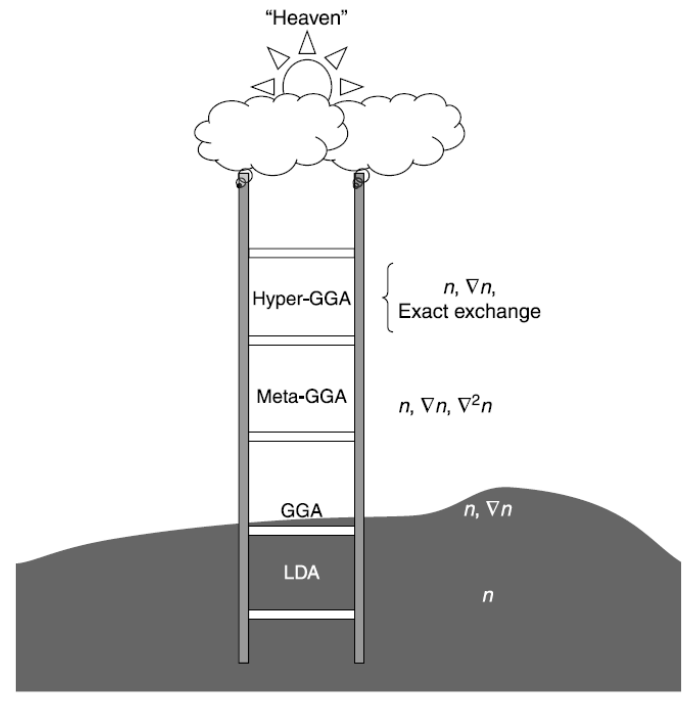
\includegraphics[height=3.5in,width=3.18in,viewport=10 5 680 700,clip]{Jacobi-ladder.png}
\caption{\small The schematic digram of Jacob's Ladder for DFT.\cite{Perdew-Schmit_2001,Science298-759_2002}}
\label{Fig:Jacob-Ladder}
\end{figure}

上述{各类}泛函%的类别})
从上到下越来越接近%化学})
精确值,因此被形象地视为``Jacob's Ladder''(登天梯,见图\ref{Fig:Jacob-Ladder}):~将\textrm{LDA~}视为第一级阶梯,\textrm{GGA~}视为第二级阶梯,更复杂的泛函形式视为第三级及更高的阶梯。\cite{PRL91-146401_2003}但在密度泛函中过度引入轨道将会%造成})
{大大增加}计算量%的大大增加})
,失去密度泛函理论对%一般})
从头计算方法的优势,因此是{并}不可取的。
下面对每一类中最重要的泛函作一些简单的介绍。

\subsection{局域密度近似和LDA泛函}
局域密度近似是Kohn和Sham提出的最简单的一种近似处理交换-相关能的方法。交换-相关能{泛函}的具体形式取为:
\begin{equation}
  \label{eq:dft-5}
E_{XC}^{LDA}[\rho]=E_X^{LDA}[\rho]+E_C^{LDA}[\rho]=\int\varepsilon_X[\rho]\rho(\vec{r}) \textrm{d}^3\vec{r}+\int\varepsilon_C[\rho]\rho(\vec{r}) \textrm{d}^3\vec{r}
\end{equation}
其中$\varepsilon_X[\rho]$和$\varepsilon_C[\rho]$分别为{一个电子的}交换能和相关能%密度})
。上式表明空间每一个点的交换能密度和相关能密度只是取决于该点的电子密度,而与其他点的电子密度无关。对{于均匀电子气,}$\varepsilon_X[\rho]$和$\varepsilon_C[\rho]$%的选取可按照均匀电子气中交换-相关能和电子密度的关系得到,})
{为常数%,等于体系的总电子交换能(或相关能)除以体系的体积和电子密度
。}对于非均匀电子气%而言})
,%这样选取的$e_X(\rho)$和$e_C(\rho)$的物理图象相当于})
{可以设想}把空间分割为无穷多个%非常})
{无限}小的区域,%假设})
{可以认为}电子的密度在每个小的区域内都是均匀的,每个小区域中的交换-相关能都%采用})
{可以按}均匀电子气%模型下})
的交换-相关能{计算},整个体系的交换-相关能就可以写成\eqref{eq:dft-5}式的形式。{采用}这种模型{,}%下的})
\textrm{Kohn-Sham~}方程的交换势表达为:
\begin{equation} \label{eq:dft-6}
V_X^{LDA}(\vec{r}) =\dfrac {\delta E_X^{LDA}}{\delta\rho(\vec{r}) }=-\dfrac 32\alpha\left\{\dfrac3\pi\rho(\vec{r}) \right\}^{1/3}
\end{equation}
Kohn和Sham等从总交换能的角度出发%给})
{得}出$\alpha=2/3$\cite{PRA140-1133_1965},Slater从交换势的角度出发,%给})
{得}出$\alpha=1$\cite{PR81-385_1951},对原子、分子体系的计算表明,选取$\alpha$约为0.7\cite{AQC6-1_1972,Slater-4_1974}结果更好。

对于用自旋密度泛函方法处理的自旋极化体系%的情况})
,%此时的})
交换能{泛函的}形式可以写成\cite{PRA20-397_1979}
\begin{equation} \label{eq:dft-7}
E_X[\rho_{\alpha},\rho_{\beta}]=\frac12E_X^{0}[2\rho_{\alpha}]+\frac12E_X^{0}[2\rho_{\beta}]
\end{equation}
其中$E_X^{0}[\rho]=E_X\bigl[\dfrac 12\rho_{\alpha},\dfrac 12\rho_{\beta}\bigr]$

相关能包含相同自旋电子间的相互作用和不同自旋电子间相互作用,不可能把相关能泛函也分解成为两种自旋电子的相关能的贡献和。一般采用Stoll\cite{TCA49-143_1978}的定义,将局域密度近似的相关能泛函写成如下形式:
\begin{equation}
  E_C=E_C^{\alpha\beta}+E_C^{\alpha\alpha}+E_C^{\beta\beta}
  \label{eq:dft-17}
\end{equation}

把局域密度近似引入自旋密度泛函理论就是通常所说的局域{自旋}密度近似(local spin-density approximation, LSDA),LSDA中的交换能{泛函}%形})
{表达}式可以%结合})
{由}\eqref{eq:dft-7}式和\eqref{eq:dft-6}式%给})
{得}出{。}相关能泛函的形式可以写成:
$$E_C^{LSDA}[\rho_{\alpha},\rho_{\beta}]=\int{\varepsilon_C(\rho,\varsigma)\rho\,\textrm{d}^3\vec{r}}$$
其中$\varsigma=(\rho_{\alpha}-\rho_{\beta})
/(\rho_{\alpha}+\rho_{\beta})
$,$\rho_{\alpha}$和$\rho_{\beta}$分别是自旋为$\alpha$和自旋为$\beta$的电子密度。均匀电子气相关能的解析形式很难求得,但是可以用数值方法计算得到%其})
数值结果,Vosko等\cite{CJP58-1200_1980}用解析式拟合%出})
精确的数值计算结果,得到局域密度近似下的相关能泛函VWN表达式{。}%但是})
他们给出的表达式%太})
{比较}复杂,Perdew和Wang\cite{PRB45-13244_1992}%又})
把它改%写})
成%为})
{比较}简单的形式,得到%的})
{一个电子的}相关能%密度})
{的}表达式为:
\begin{equation}
  \label{eq:dft-8}
\varepsilon_C^{LDA}(r_s,\varsigma)=\varepsilon_C^{LDA}(r_s,0)+a_C(r_s)\dfrac{f(\varsigma)}{f''(\varsigma)}(1-\varsigma^4)+[\varepsilon_C(r_s,1)-\varepsilon_C(r_s,0)]f(\varsigma)\varsigma^4
\end{equation}
其中$r_s=\left[\dfrac 3{4\pi}\bigl(\rho_{\alpha}+\rho_{\beta}\bigr)\right]^{-1/3}$,$f(\varsigma)=[(1+\varsigma)^{4/3}+(1-\varsigma)^{4/3}-2]/(2^{4/3}-2)$,\\$\varepsilon_C(r_s,0)$,$\varepsilon_C(r_s,1)$和$-a_C(r_s)$由经验公式
$$G(r_s,A,\alpha_1,\beta_1,\beta_2,\beta_3,\beta_4,p)=-2A(1+\alpha_1r_s)\ln\left[1+\dfrac1{2A(\beta_1r_s^{1/2}+\beta_2r_s+\beta_3r_s^{3/2}+\beta_4r_s^{p+1})}\right]$$
计算{,}其中{$G$可以是$\varepsilon_C(r_s,0)$,$\varepsilon_C(r_s,1)$或$-a_C(r_s)$},$A$,$\alpha_1$,$\beta_1$,$\beta_2$,$\beta_3$,$\beta_4$,$p$%都})
是{特定的}参数。

由于局域密度近似下的交换-相关能泛函形式是从均匀电子气模型中得到的,一般认为它对于电子密度变化比较小的体系结果比较好,%而})
{可能}不适用于电子密度剧烈变化的原子、分子和一些固体体系。%事实上})
{不过},局域密度近似用于原子、分子特别是某些扩展体系仍能得到很合理的结果,其原因是%因为})
局域密度近似下的交换-相关能密度和交换-相关孔在每一点上的数值都来自一个体系的精确的值,因此满足交换-相关电荷总量为一个电子电荷的负值的约束条件,交换-相关能泛函的误差%在不同位置})
{能部分}相互抵消。

\subsection{梯度校正和GGA泛函}
%由于})
LDA是建立在均匀电子气模型基础上{的},而原子、分子和很多扩展体系的电子密度远非均匀,%通常})
由LDA计算得到的分子的原子化能{通常}过大。%要})
{为}进一步提高计算精度,%就})
需要对电子密度的非均匀性加以校正。一般是通过在交换-相关能泛函中引入电子密度%的})
梯度来加以校正{,}即构造GGA泛函。可以将GGA交换能泛函写成一般形式:
\begin{equation}
  E_X^{GGA}=E_X^{LDA}-\sum_{\sigma}\int F[x_{\sigma}]\rho_{\sigma}^{\frac43}(\vec r)\textrm{d}^3r{=E_X^{LDA}+E_X^{NL}}
  \label{eq:dft-18}
\end{equation}
其中$x_{\sigma}=|\nabla\rho_{\sigma}|\rho_{\sigma}^{-4/3}$称为约化梯度,是一个无量纲的量。%依据})
{按}所用$F${泛函}的形式不同,%目前})
{现有}GGA的交换能泛函可以分为两大类,一类以Becke\cite{PRA38-3098_1988}在1988年提出的表达式为基础:
\begin{equation}
  \label{eq:dft-9}
E_X^{NL}=-b\sum_{\sigma}\int\rho_{\sigma}^{4/3}\dfrac{x_{\sigma}^2}{1+6bx_{\sigma}\sinh^{-1}x_{\sigma}}\textrm{d}^3r
\end{equation}
其中$b$\,=\,0.0042{。}%$X_{\sigma}=|\nabla\rho_{\sigma}|\rho_{\sigma}^{-4/3}$})
这是目前常用的交换能非局域校正公式。属于这一类的交换能泛函有PW91\cite{PRB46-6671_1992,PRB48-4978_1993,PRB54-16533_1996,PRB57-14999_1998}、FT97\cite{MP91-847_1997}、CAM(A)和CAM(B)\cite{JCP99-8765_1993}等等。另一类泛函的$F${泛函}采用有理函数{形式,}包括幂函数和有理分式的泛函。属于这一类的交换能泛函有B86\cite{JCP84-4524_1986}、P86$_x$\cite{PRB33-8800_1986}、LG\cite{PRA47-4681_1993}、PBE\cite{PRL77-1396_1996,IBID78-1396_1997}、VSXC\cite{JCP109-400_1998}等。B86采用的$F${泛函}的形式是
\begin{equation}
  F^{B86}=\left[1+1.296\left(\dfrac{x_{\sigma}}{(24\pi^2)^{1/3}}\right)^2+14\left(\dfrac{x_{\sigma}}{(24\pi^2)^{1/3}}\right)^4+0.2\left(\dfrac{x_{\sigma}}{(24\pi^2)^{1/3}}\right)^6\right]^{1/15}
  \label{eq:dft-19}
\end{equation}

最常用的相关能非局域校正{$E_C^{NL}$}是Perdew和Wang\cite{PRB33-8822_1986}提出的%形})
{表达}式以及把$E_C^{NL}$和$E_C^{LDA}$合{并}在一起计算的LYP%形})
{表达}式\cite{PRB37-785_1988}。Perdew和Wang的表达式为:
\begin{equation} 
  \label{eq:dft-10}
E_C^{NL}=\int{d^{-1}\textrm{e}^{-\varphi}C[\rho]|\nabla\rho|^2\rho^{-4/3}\textrm{d}^3r}
\end{equation}
其中$\varphi=1.745\times 0.11\times C[\infty]|\nabla\rho|/(C[\rho]\rho^{7/6})$,%\\%\linebreak

$d=2^{1/3}\left[\biggl(\dfrac {1+\varsigma}2\biggr)^{5/3}+\biggl(\dfrac{1-\varsigma}2\biggr)^{5/3}\right]^{1/2}$,

$C[\rho]=a+(b+ar_s+\beta r_s^2)(1+\gamma r_s+\delta r_s^2+10^4\beta r_s^3)^{-1}$,\\%\linebreak
$a$,$b$,$\alpha$,$\beta$,$\gamma$,$\delta$为通过拟合{实验数据}得到的参数。

LYP相关能泛函是%利用})
{在}Colle-Salvetti公式\cite{TCA37-329_1975}{的基础上}导出的,其具体形式为:
\begin{equation}
  \begin{aligned}
  E_C^{LYP}=&-a\int\dfrac{\gamma(\vec r)}{1+d\rho^{-1/3}}\biggl\{\rho+2b\rho^{-5/3}\biggl[2^{2/3}C_F\rho_{\alpha}^{8/3}+2^{2/3}C_F\rho_{\beta}^{8/3}-\rho t_w\biggr.\biggr.\\
  &+\left.\left.\dfrac19\left(\rho_{\alpha}t_w^{\alpha}+\rho_{\beta}t_w^{\beta}\right)+\dfrac1{18}\left(\rho_{\alpha}\nabla^2\rho_{\alpha}+\rho_{\beta}\nabla^2\rho_{\beta}\right)\right]\textrm{e}^{-c\rho^{-1/3}}\right\}\textrm{d}\vec r
  \end{aligned}
  \label{eq:dft-20}
\end{equation}
其中$\gamma(\vec r)=2\left[1-\dfrac{\rho_{\alpha}^2(\vec r)+\rho_{\beta}^2(\vec r)}{\rho^2(\vec r)}\right]$,$t_w(\vec r)=\dfrac18\cdot\dfrac{|\nabla\rho(\vec r)|^2}{\rho(\vec r)}-\dfrac18\nabla^2\rho(\vec r)$,$C_F=\dfrac3{10}(3\pi^2)^{2/3}$,\\$a$,$b$,$c$,$d$%是})
{为通过拟合实验数据确定的}常数。

\subsection{\textit{meta}-GGA泛函}
由于密度泛函理论的交换-相关能中包含了实际体系与无相互作用参考体系动能{之}间的差别,%因此如果})
在交换和相关能泛函中包含动能密度$\tau$,%则})
计算结果可能会更合理一些。表达式中包含动能密度$\tau$为变量的泛函称为\textit{meta}-GGA泛函。动能密度的一般定义为
\begin{equation}
  \tau=\sum_i^{occ}|\nabla\Psi_i|^2
  \label{eq:dft-21}
\end{equation}
其中$\Psi_i$是含自旋的轨道。

van~Voorhis和Scuseria于1998年提出了基于密度矩阵展开理论\cite{PRC5-1472_1972,PRC11-1030_1975}的VSXC泛函\cite{JCP109-400_1998},得到的交换能密度泛函为:
\begin{equation}
  \begin{aligned}
    E_X[\rho_{\alpha},\rho_{\beta}]&=\sum_{\sigma}\int\rho_{\sigma}^{4/3}{f(x_{\sigma},z_{\sigma})
    }\textrm{d}\vec r\\
    f(x_{\sigma},z_{\sigma})&=\left(\dfrac a{\Gamma_{\sigma}(x,z)}+\dfrac{bx_{\sigma}^2+cz_{\sigma}}{\Gamma_{\sigma}^2(x,z)}+\dfrac{dx_{\sigma}^4+ex_{\sigma}^2z_{\sigma}+f_0z_{\sigma}^2}{\Gamma_{\sigma}^3(x,z)}\right) 
  \end{aligned}
  \label{ed:def-22}
\end{equation}
其中$x_{\sigma}=|\nabla\rho_{\sigma}|\rho_{\sigma}^{-4/3}$,$z_{\sigma}=\tau\rho_{\sigma}^{-5/3}-C_F$,$C_F=\dfrac35(3\pi^2)^{2/3}$,$\Gamma_{\sigma}(x,z)=1+\alpha(x_{\sigma}^2+z_{\sigma})$,\linebreak $\alpha$为常数;$a$,$b$,$c$,$d$,$e$,$f_0$均为参数。

{在}相关能泛函的计算中,将相同自旋电子的相关作用和不同自旋{电子}的相关作用分开%计算})
{处理}\cite{TCA49-143_1978},%有})
\begin{equation}
  \begin{aligned}
    E_C=&E_C^{\alpha\beta}+E_C^{\alpha\alpha}+E_C^{\beta\beta}\\
    E_C^{\sigma\sigma'}=&\int f^{\sigma\sigma'}(x,z)e_{c\sigma\sigma'}^{LDA}\textrm{d}\vec r\\
    E_C^{\sigma\sigma}=&\int f^{\sigma\sigma}(x_{\sigma},z_{\sigma})
    D_{\sigma}e_{c\sigma\sigma}^{LDA}\textrm{d}\vec r
  \end{aligned}
  \label{eq:dft-23}
\end{equation}
其中$x^2=x_{\alpha}^2+x_{\beta}^2$,$z=z_{\alpha}+z_{\beta}$,{$e_C^{LDA}$为相关能密度,}$D_{\sigma}$是相同自旋自相互作用的校正系数,表达式为:
$$D_{\sigma}=1-\dfrac{x_{\sigma}^2}{4(z_{\sigma}+C_F)}$$

1989年Becke和Roussel从类氢原子的密度矩阵表达式出发,提出%了})
BR89交换能泛函\cite{PRA39-3761_1989}。
交换势为:
$$U_{X\sigma}=-4\pi\int_0^{\infty}\rho_X^H(a,b,s)s\textrm{d}s=-\left(1-\textrm{e}^{-x}-\frac12x\textrm{e}^{-x}\right)/b$$
其中$\rho_X^H(a,b,s)$是类氢原子的交换孔函数,%$x$})
{$x=ab$},由{逐点求解}超越方程
$$\dfrac{x\textrm{e}^{-2/3}}{x-2}=\dfrac23\pi^{2/3}\dfrac{\rho_{\sigma}^{5/3}}{Q_{\sigma}}$$
%逐点求解})
得到。方程中$Q_{\sigma}$\,=\,$\dfrac16\left[\nabla^2\rho_{\sigma}-2\gamma\bigl(\tau_{\sigma}-\dfrac{(\nabla\rho_{\sigma})^2}{4\rho_{\sigma}}\bigr)\right]$,其中$\gamma$是参数,$\tau_{\sigma}$为动能密度{,}\linebreak $b$%根据})
\,=\,$\left[\dfrac{x^3\textrm{e}^{-x}}{8\pi\rho_{\sigma}}\right]^{1/3}$%计算得到})
{,$a=x/b$。}%最后得到})
总的交换能为:$E_{X\sigma}=\dfrac12\displaystyle\int\rho_{\sigma}U_{X\sigma}\textrm{d}\vec r$

对于分子体系,交换孔函数比较离域,BR89模型往往高估交换能密度,Becke用LDA动能与精确动能密度的比值为参数,提出了B00修正模型\cite{JCP112-4020_2000}。修正后的交换能泛函形式为:
\begin{equation}
  E_{X\sigma}^{BR89}=\int e_{X\sigma}^{BR89}[1+f_{X\sigma}(t_{\sigma})
  ]\textrm{d}\vec r
  \label{eq:dft-24}
\end{equation}
其中$f_{X\sigma}$是校正函数,$e_{X\sigma}^{BR89}$是BR89模型中的交换能密度。$f_{X\sigma}(t_{\sigma})=a_t(\omega_{\sigma}-2\omega_{\sigma}^3+\omega_{\sigma}^5)$,$\omega_{\sigma}=\dfrac{t_{\sigma}-1}{t_{\sigma}+1}$,$t_{\sigma}=\dfrac{\tau_{\sigma}^{LSDA}}{\tau_{\sigma}^{exact}}$,式中$a_t$为经验参数。

%若})
加上{电子}相关{能}作用(采用Bc88相关能泛函\cite{JCP88-1053_1988})
,得到的交换-相关能{泛函的}表达式为:
\begin{equation}
  E_{XC}=E_X^{BR89}+c_{opp}E_{Copp}^{Bc88}+c_{par}E_{Cpar}^{Bc88}+a_{mix}\sum_{\sigma}\int e_x^{BR89}f_{x\sigma}(t_{\tau})\textrm{d}\vec r
  \label{eq:dft-25}
\end{equation}
其中$E_{Copp}^{Bc88}$和$E_{Cpar}^{Bc88}$分别是自旋平行、反平行的相关能。拟合得到的参数$a_{mix}$的优选值为0.135。

\subsection{{杂化(hybrid)}泛函}
%还有})
{目前}一种很常用的交换-相关能{泛函}是%采用})
把Hartree-Fock%的相关})
{交换}能%形式})
与近似%的})
交换-相关能%相})
混合%的方法})
\cite{JCP104-1040_1996,JCP98-5648_1993},其表达式%可以写})
为:
\begin{equation}
E_{XC}^{hybrid}=\alpha E_X+(1-\alpha)\bar{E}_X+\bar{E}_C
 \label{eq:dft-11}
\end{equation}
其中$E_X$是Hartree-Fock%的相关})
{交换}能%形式})
,$\bar{E}_X$和$\bar{E}_C$分别为近似的交换能和相关能泛函,通常$\alpha$取值为0.28左右。%例如})
“半对半(half and half)”泛函\cite{JCP98-1372_1993}%,其})
{的}表达式%可以写成})
{为}:
\begin{equation}
  E_{XC}^{HH}=\dfrac12E_{X}^{HF}+\dfrac12E_{XC}^{LSDA}
  \label{eq:dft-26}
\end{equation}

杂化型的密度泛函方法可以统一地归为一类,称为绝热关联方法(Adiabatic Connection Method, ACM)。所谓绝热关联,就是定义以$\lambda$为参量的Hamiltonian
\begin{equation}
  \hat H_{\lambda}=-\dfrac12\sum_i\nabla_i^2+\sum_iV_i(\rho,\lambda)+\dfrac{\lambda}2\sum_{i\neq j}\dfrac1{r_{ij}}
  \label{eq:dft-27}
\end{equation}
其中$V_i(\rho,\lambda)$是与$\lambda$有关的外势,选择$V_i(\rho,\lambda)$使不同$\lambda$时的密度$\rho$保持恒定。%显然})
当$\lambda$=0时对应于无相互作用参考体系;而当$\lambda$=1时对应%着})
真实体系。当$\lambda$连续地从0变化到1时,无相互作用参考体系绝热地过渡到真实体系。利用一级微扰理论\cite{JCP88-1053_1988},可以得到交换-相关能%地})
{的}表达式为:
$$E_{XC}=\dfrac12\int\rho(\vec r)d\vec r\int\dfrac{\bar h_{xc}(\vec r,\vec r\,')}{|\vec r-\vec r\,'|}\textrm{d}\vec r\,'$$
其中$$\bar h_{xc}(\vec r,\vec r\,')=\int_0^1h_{xc}^{\lambda}(\vec r,\vec r\,')\textrm{d}\lambda$$
$h_{xc}^{\lambda}(\vec r,\vec r\,')$是与$\hat H_{\lambda}$相应的交换-相关孔函数。令
$$U_{XC}^{\lambda}=\dfrac12\int\rho(\vec r)d\vec r\int\dfrac{h_{xc}^{\lambda}(\vec r,\vec r\,')}{|\vec r-\vec r\,'|}\textrm{d}\vec r\,'$$
于是有$$E_{XC}=\int_0^1U_{XC}^{\lambda}\textrm{d}\lambda$$
如果%选用最})
简单%的})
{地}假设,%认为})
$U_{XC}^{\lambda}$与$\lambda$满足线性关系,就%可以})
得到
$$E_{XC}=\dfrac12U_{XC}^0+\dfrac12U_{XC}^1=\dfrac12E_X^{HF}+\dfrac12U_{XC}^1$$
这就是“半对半(half and half)”泛函以及%所有})
{其它}杂化型泛函的理论基础。

属于这一类的泛函还有B3P\cite{JCP98-5648_1993}、B3LYP\cite{JPC98-11623_1994}、B1B95\cite{JCP104-1040_1995}、B97\cite{JCP107-8554_1997}、B98\cite{JCP109-2092_1998}、PBE0\cite{JCP110-6158_1999}~等。其中最流行的B3LYP泛函的具体形式为:
$$E_{XC}^{B3LYP}=(1-a)E_X^{LSDA}+aE_X^{HF}+bE_X^{B88}+cE_C^{LYP}+(1-c)E_C^{LSDA}$$
其中$a$,$b$,$c$%均})
为参数。

%一般来说})
这几种泛函的近似公式的计算结果{一般}差别并不很大,对各种近似泛函的计算结果可以参考文献\inlinecite{JCP98-5612_1993,CPL316-160_2000}。

由于原子中的电子密度的不均匀性比分子中的不均匀性更强,交换-相关能的梯度校正部分对原子{计算}影响比较大,%能够})
比较明显%的})
{地}降低原子的能量,而对分子{计算}影响较小{。}与LDA的结果相比,交换-相关能的梯度校正使得分子的原子化能{计算值}降低,键长{计算值}增加,总体%上得到的})
{看计算}结果%也})
有明显改善。%也正是这些})
精度较高的交换-相关能泛函%形式})
的提出,使%得})
密度泛函理论%能够广泛应用于定量研究})
{在}原子、分子、团簇和固体等%各种})
体系的%性质。})
{定量研究中得到广泛的应用并且得到满意的结果。}

有必要指出的是,目前使用的{近似能量}泛函%形式})
还存在问题,比较集中的有:
\begin{enumerate}
	\item 自相互作用抵消不干净;
	\item 对于简并基态和近简并基态还存在%严重问题})
{难于合理解决的困难};
	\item 对于弱相互作用体系,如van der Waals相互作用不能忽略时,{计算结果}还有很大的误差。%由于})
\end{enumerate}
电子与{其}自身没有相互作用,因此交换-相关能中包含的电子自相互作用部分应该和电子间Coulomb能中包含的自相互作用部分完全抵消,而目前使用的{近似能量密度}泛函%形式})
都不%具有})
{严格满足}这个%特点})
{条件},因此{用}密度泛函方法计算电子数很少的体系一般都会有比较大的误差。{在体系处于}简并基态和近简并基态的%问题一直是密度泛函理论比较困难的部分})
{情况下},当%体系的})
基态电子密度%取自})
{用}不同的简并轨道{计算}时%密度泛函方法得到的})
体系能量应该%保持一致})
{不变},%现在的})
{而现有近似能量密度}泛函%形式也})
不具有这个%特点})
{性质},%由于多数原子的基态是简并的,})
用%密度泛函方法})
{来}计算%的})
原子基态能量就%会})
随%着选})
取%的})
不同简并原子轨道{计算电子密度}而不同\cite{PRB43-6865_1991,CPL265-481_1997},%这})
给计算分子体系的原子化能造成很大%的})
困难。密度泛函方法计算弱相互作用体系出现%问题})
的{困难}主要%原因})
是弱相互作用体系%通常键})
{中的相互作用}能和现%在所用的近似泛函形式})
{有近似能量密度泛函}本身的{计算}误差%可以相比})
{在同一量级}。%但是})
寻找精度%有})
明显提高的近似能量密度泛函%形式})
是难度很大的工作,目前常用的{近似能量密度}泛函%形式})
主要是二十世纪八十年代后期和九十年代初提出的,此后虽然%也有一些})
{提出过很多}近似{能量密度}泛函%形式被提出来})
,%但是})
与以前提出的%泛函形式})
相比%都})
{精度并}没有很明显的%改进})
{提高}。


\chapter{周期势与计算方法}
能带理论是凝聚态物理中最重要的理论之一,它是量子力学确立后,在研究金属电导理论过程中发展起来的,已经成为固体电子理论的支柱。理想晶体的原子有序排列成晶格,具有平移周期性,势能$V(\vec r)$满足:
\begin{equation}\label{eq:solid-2}
	V(\vec r)=V(\vec r+\vec R_n)\quad\mbox{($\vec R_n$为任意格矢)}
\end{equation}
\textrm{Bl\"och}定理指出:
{\it 对于具有周期性的势场,单电子的Schr\"odinger方程}
\begin{equation}\label{eq:solid-1}
  \biggl[-\dfrac{\hbar^2}{2m}\nabla^2+V(\vec r)\biggr]\psi=E\psi
\end{equation}
{\it 的解满足}
\begin{equation}
  \psi(\vec r+\vec R_n)=e^{i\vec k\cdot\vec R_n}\psi(\vec r)
  \label{eq:bloch}
\end{equation}
$k$是与平移对称性相应的量子数,因此理想晶体的电子波函数除了与势函数具有相同的平移周期性,还受到平面波的相位控制。密度泛函理论发展起来之后,为包括能带计算在内的电子结构模拟提供了坚实的基础,可以通过选定交换-相关泛函(主要是LDA或GGA),自洽迭代求解Kohn-Sham方程直接得到电子能带。在具体应用DFT求解能带时,除了泛函的选择,还需要考虑各种近似,不同近似方法的差别在于单电子有效势和波函数形式的选取两方面。

\section{Muffin-Tin近似与非Muffin-tin校正}
周期体系的势函数与一般原子、分子不同,集中在原子间区域,波函数较为平缓,并且有周期特征,如图\ref{Potential-Wave}所示:
\begin{figure}[h!]
\centering
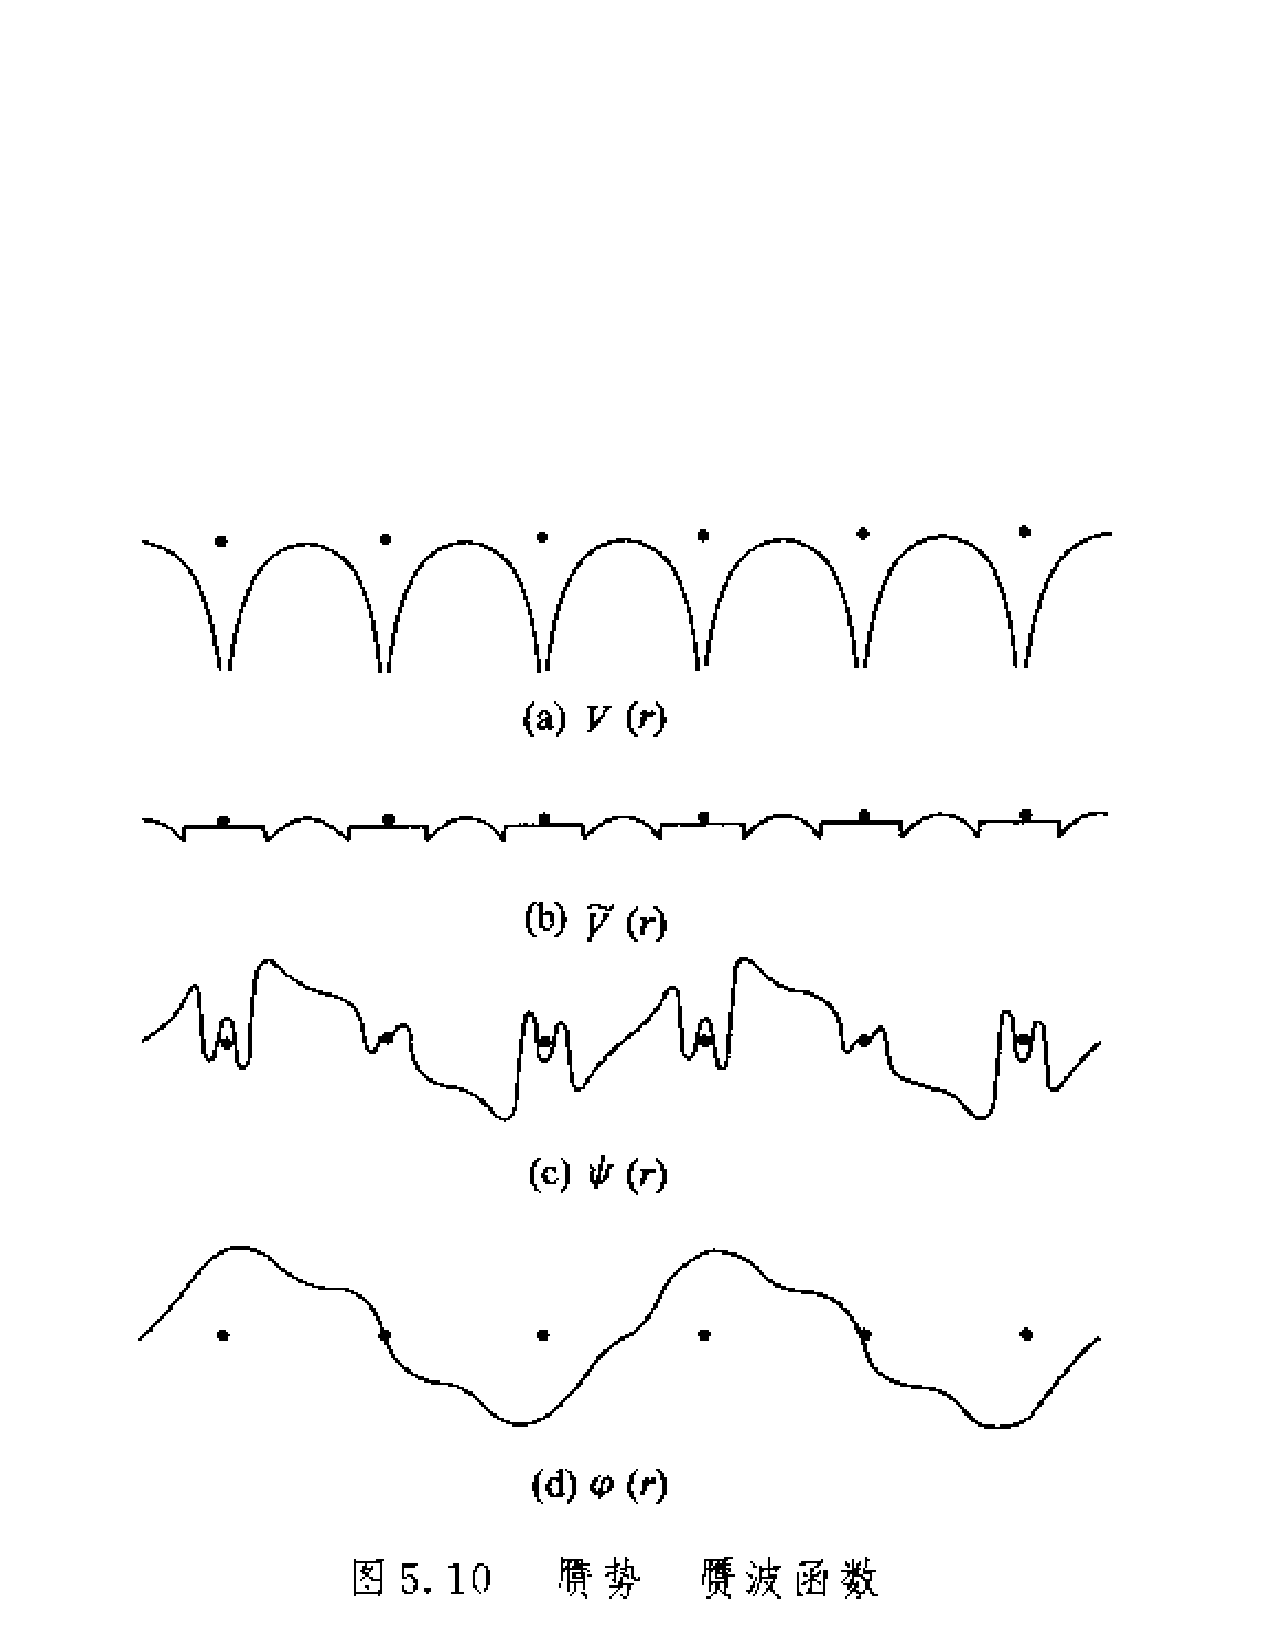
\includegraphics[height=0.8in,width=4.in,viewport=41 458 539 546,clip]{Pseudo_wave.pdf}\\
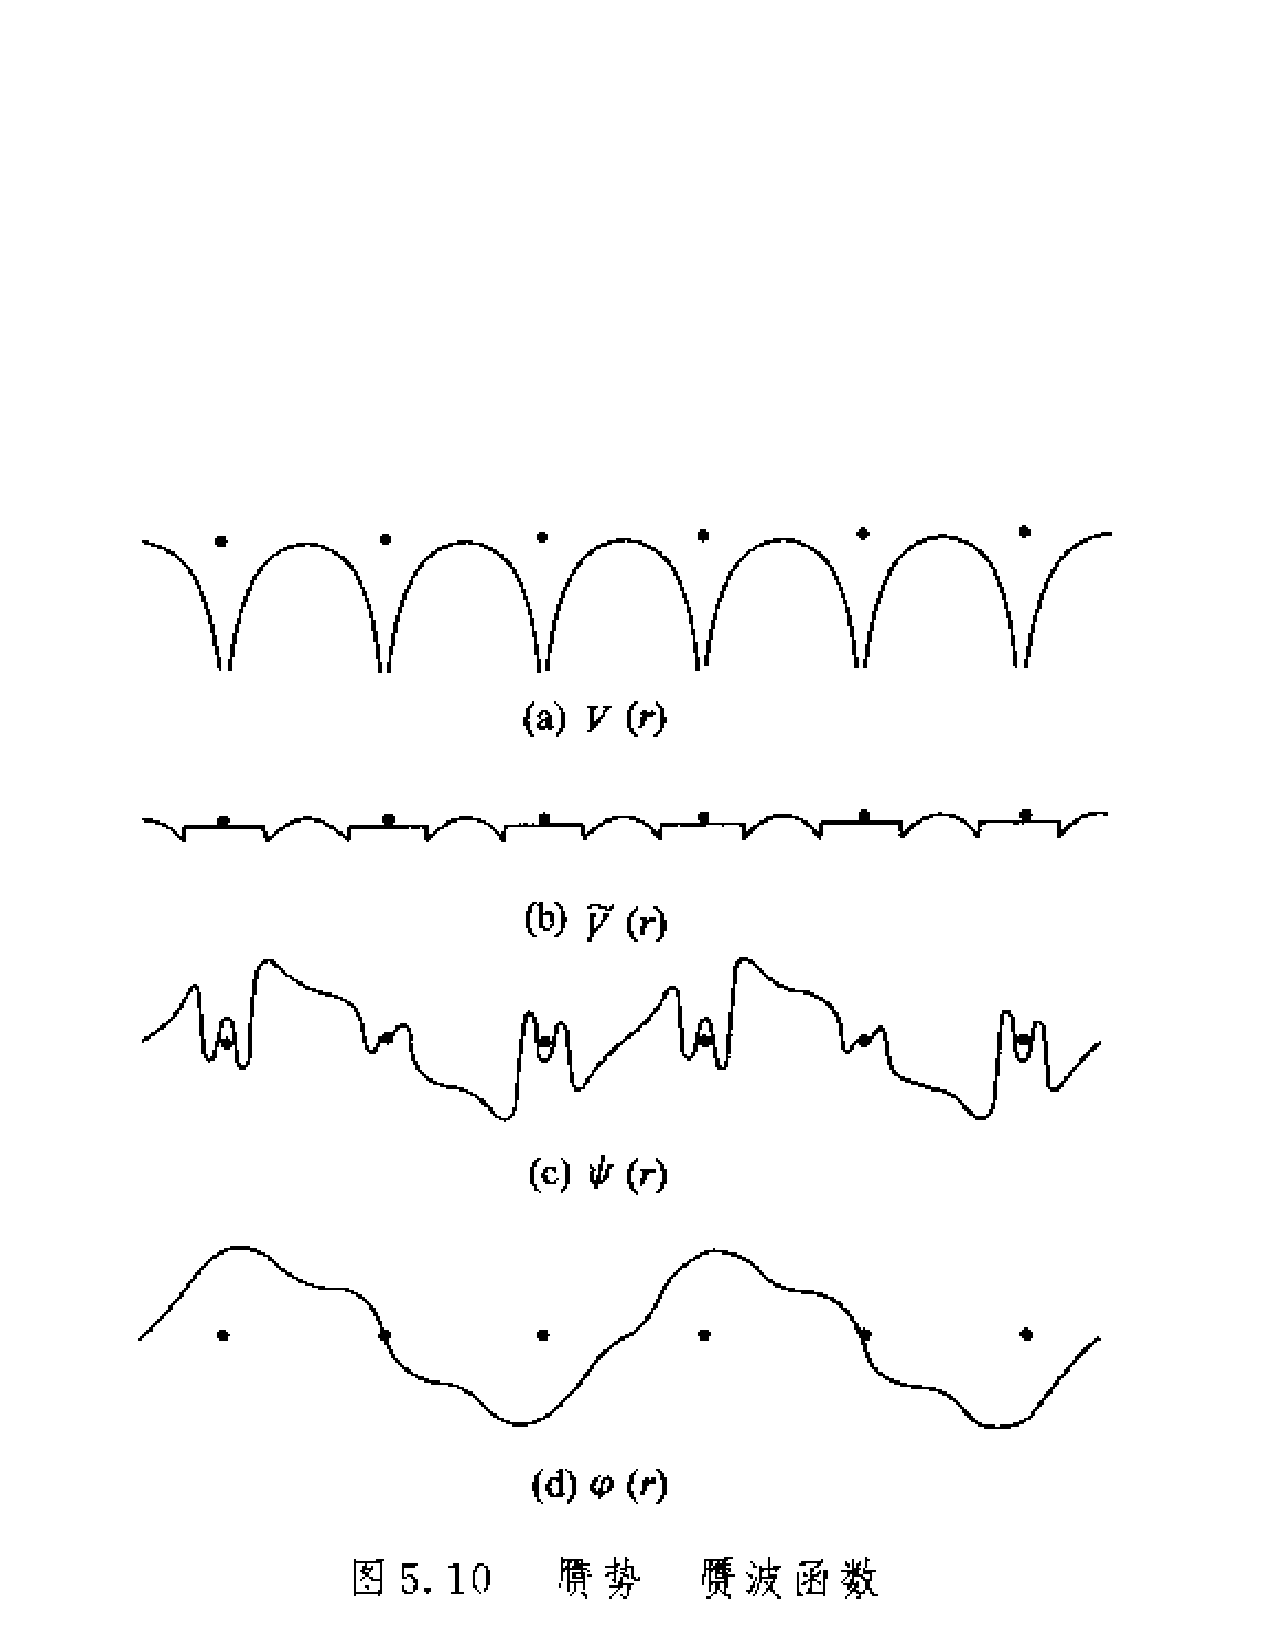
\includegraphics[height=0.8in,width=4.in,viewport=41 238 539 339,clip]{Pseudo_wave.pdf}
\caption{\small \textrm{The periodic Potential (up) and the wave functions (down) in crystal.}}%(与文献\cite{EPJB33-47_2003}图1对比)
\label{Potential-Wave}
\end{figure}
最早的能带计算方法是Wigner-Seitz(WS)原胞方法\cite{PR43-804_1933},没有特别考虑周期特征。该方法假定晶体势场有球对称性,即$V(\vec r)=V(r)$,波函数为中心力场Schr\"odinger方程标准的线性组合,边条件为$\left(\dfrac{\partial\psi_{\vec k}(r)}{\partial r}\right)_{r_0}$,$r_0$为球半径。该方法在碱金属能带计算取得了很大的成功。将原胞简化为球,结果仅依赖于每个原子平均占据的体积,忽略实际晶体结构的影响。如果采用真实的多面体WS原胞,为了满足表面边边界条件,计算将变得十分复杂,同时也会导致中心力场在原胞边界上导数的不连续。为了克服WS原胞方法的缺陷,1937年,Slater提出Muffin-Tin(MT)近似\cite{PR51-846_1937}。MT近似的主要思想是将WS原胞分为两个区域,一个是以原胞中的每个原子{\it i}\,为中心,半径为$r_i$的彼此不相交叠的球形区,此区域内具有球对称性势$V(r_i)$,在接近原子核区域,势能变化非常较大;球形区以外为第二部分(间隙区),此处势能近似为一常数,如图\ref{Muffin_tin-1}所示:
\begin{figure}[h!]
\centering
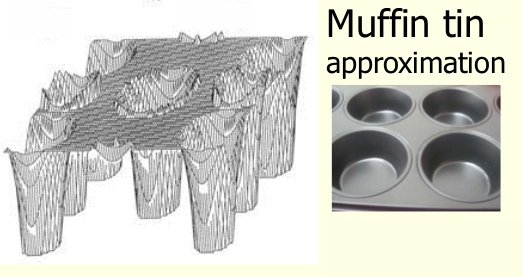
\includegraphics[height=1.45in,width=1.92in,viewport=1 22 317 295,clip]{Muffin-tin.png}
\includegraphics[height=1.45in,width=1.92in,viewport=1 20 515 435,clip]{Muffin-Tin.png}
\caption{\small \textrm{Division of the unit cell into spheres(I) and into interstitial region(II)}}%(与文献\cite{EPJB33-47_2003}图1对比)
\label{Muffin_tin-1}
\end{figure}

\begin{equation}
  V(\vec r)=\left\{
  \begin{aligned}
    &V(r),\quad&r\leqslant R_{MT} \\
    &V_c.&r>R_{MT}
  \end{aligned}\right.
  \label{eq:Muffin-Tin}
\end{equation}
为简化计算,通常取$V_c$=0,这等价于将晶体的势能零点移动到$V_c$位置上。MT势比原胞法相更接近实际情况,适用性更强,即使对于晶体势场不能完全用MT势描述的情况,如球内的非球形对称部分不能完全忽略的情况,也可以通过适当的方法修正。

为了计算周期性晶体势场,Mattheiss提出了一个构造MT势的方法,在中心原子的势场上叠加上周围原子势场以中心为原点的球谐函数展开的球对称部分\cite{PRA133-1399_1964}。将Coulomb势和交换项分开处理。Coulomb势用晶体中原子势的静电排斥叠加表示,临近原子的Coulomb势叠加用L\"owdin发展的$\alpha$展开方法计算:
\begin{equation}
  V_C(r)=\sum_i\dfrac{N_i}{2a_ir}\int_{|a_i-r|}^{|a_i+r|}r'V_C^{at}(r')dr'
  \label{eq:lodin-alpha}
\end{equation}
其中$a_i$是第$i$个等同原子球的半径;$N_i$是第$i$个原子的等同原子球数目;$V_C^{at}(r)$是原子的Coulomb势,可用下式%\eqref{eq:atomic-coulomb}
计算:
\begin{equation}
  V_C^{at}(r)=-\dfrac{2Z}r+\frac2r\int_0^r4\pi\rho^{at}(r')r'^2dr'+2\int_r^{\infty}4\pi r'\rho^{at}(r')dr'
  \label{eq:atomic-coulomb}
\end{equation}
其中$\rho^{at}(r)=\sum\limits_l n_lu_l^2$是自洽的原子电荷密度,$n_l$是占据电子数,$u_l$是自洽原子波函数\cite{Herman-Skillman}。对于含有重元素的体系,$u_l$的计算可参考文献\inlinecite{PR137-23_1965}。由此得到的MT势为
\begin{equation}
  V_{MT}(r)=V_C^{at}(r)+\sum_i\dfrac{N_i}{2a_ir}\int_{|a_i-r|}^{|a_i+r|}r'V_C^{at}(r')dr'+V_{xc}(r)-V_c
  \label{eq:potential-MT}
\end{equation}
最初的交换势$V_{xc}$贡献用Slater的$\chi_{\alpha}$方法计算\cite{PR81-385_1951},现在则根据选定的交换-相关泛函给出。计算时$\rho(r)$取晶体的空间电荷密度,初始值为中心原子的电子密度叠加相邻原子的电子密度。$V_c$是MT球间常数势。对单原子金属体系,WS原胞内的MT球间常数势为
\begin{equation}
  V_c=\dfrac3{R_{WS}^3-R_{MT}^3}\int_{R_{MT}}^{R_{WS}}V_{MT}(r)dr
  \label{eq:monoatomic-ini}
\end{equation}
这里$R_{WS}$由$(4/3)\pi R_{WS}^3=\Omega_0$计算得到,$\Omega_0$是原胞体积。

MT近似方法主要适用于具有密堆积的简单晶格的单原子(过渡)金属\cite{SSP26-104_1971},但对于非密堆积的金属化合物(如体心立方的CsCl结构)\cite{PRB13-5362_1976}的计算结果不理想,因为在化合物中原胞电中性条件无法保证。对于这类含有复式晶格的体系,必须采用另外的方法计算\cite{PSSB36-447_1969}。
%与简单晶格计算方法相比,复式晶格计算中叠加的是位于不同中心的电子密度而不再是原子势,并利用元胞的电中性假设,求出MT球间的常数电荷。确定电荷密度之后,利用Poisson方程求解MT球内势能和球间的常数势$V_c$。

%复式晶格的电子密度表示
%\begin{equation}
%  \rho_s(r)=\rho_s^{at}(r)+\sum_{mj}\dfrac{n_{mj}}{2a_{mj}r}\int_{|a_{mj}-r|}^{|a_{mj}+r|}\rho_m^{at}(r')r'dr'
%  \label{eq:equation-58}
%\end{equation}
%这里$\rho_s^{at}(r)$是$s$原子的电子密度;$r=|\vec r-\vec{\tau}_j|\leqslant R_{MT}^s$;$\vec{\tau}_j$是第$j$个等同原子球心位置;$n_{mj}$是中心在$\tau_j$矢径为$a_{mj}$的等同原子$m$的数目。WS原胞MT球外的常数电荷由复式原胞的电中性条件确定。
%\begin{equation}
%  \rho_c=\dfrac{\sum_i(Z_i-Q_i)}{\Omega_0-\sum_i\Omega_i}
%  \label{eq:solid-59}
%\end{equation}
%其中$Q_i=4\pi\int_0^{R_i}\rho_i(r)r^2dr$,$\Omega_i$是球心位于$\vec{\tau}_i$的球体积。在复式晶格内,根据周期性边界条件求解Poisson方程得到球对称晶体势,并对角度求和
%\begin{equation}
%  \begin{split}
%   V_s(r)=&-\frac{2Z_s}r+\frac{8\pi}r\int_0^r\rho_s(r')r'^2dr'+8\pi\int_r^{R_{MT}^s}\rho_s(r')r'dr' \\
%   &-2\sum_j(Z_j-Q_j+\rho_c\Omega_j)\varphi(\vec{\tau}_j-\vec{\tau}_s)-4\pi\rho_c(R_{MT}^s)^2 \\
%   &+\frac{(4\pi)^2}{3\Omega_0}\sum_j\int_0^{R_{MT}^s}[\rho_j(r')-\rho_c](r')^4dr'
%  \end{split}
%  \label{eq:solid-60}
%\end{equation}
%MT间的常数势根据式\eqref{eq:solid-61}确定:
%\begin{equation}
%  \begin{split}
%    V_c=&\frac2{\Omega_0-\sum_j\Omega_j}\left[\frac32\sum_j\frac{\Omega_j}{R_j}\left(Z_j-Q_j+\frac56\rho_c\Omega_j\right)\right.\\
%    &+\left.\sum_{ij}\Omega_j(Z_i-Q_i+\rho_c\Omega_i)\varphi(\vec{\tau}_i-\vec{\tau}_j)\right] \\
%    &+\frac{(4\pi)^2}{3\Omega_0}\sum_j\int_0^{R_{MT}^s}[\rho_j(r')-\rho_c](r')^4dr'
%  \end{split}
%  \label{eq:solid-61}
%\end{equation}
%这里$\varphi(\vec{\tau}_i-\vec{\tau}_j)$是位于$\vec{\tau}_j$的$j$离子静电势;$R_{MT}^s$是第$s$个MT球的半径。该球内的势能
%\begin{equation}
%  V_{MT}^s(r)=V_s(r)+V_{xc}(r)-V_c
%  \label{eq:solid-62}
%\end{equation}

%此外,晶体中离子(实)间的相互作用用Madelung势表示,对大多数晶体来说,晶体的Madelung势是已知的。需要指出的是,采用MT近似计算,正确选择MT球半径非常重要,因为球半径选择对于势能的Coulomb势和MT球内的电子电荷有重要影响。%对于WS原胞内含有两个原子的体系,MT球半径的选择使得两个MT球相切位置的MT势\eqref{eq:solid-62}相等。

使用MT近似方法,MT球外的势能是一常数,但实际上要求%如果MT球外有非零的电子密度,无法通过MT近似构造出与此电荷密度一致的势能。假设MT球外的电荷满足式\eqref{eq:solid-59},
求解Possion方程所得到的势能$V_c$并非是一常数,而与位置有关。所以应用MT近似,假设$V_c$为一常数,是MT近似误差的主要来源。

%\subsection{非MT校正}
关于MT近似的改进方法有许多\cite{RPP44-139_1981}。考虑对MT近似的修正,主要有两类方案。一种是在推导Hamiltonian的基函数时考虑非MT效应;另一种采用MT近似构造基函数,但对势能进行非MT修正。一般来说主要应用第二种方案,构造一般形式的势能。在MT近似下,WS原胞分为球形区(S)和间隙区(I)两部分。对这两部分区域,非MT校正分别采用了不同形式的校正形式。一般地,在MT球内,晶体势用球谐函数(或者是满足晶体对称性的球谐函数),MT球外的势能用Fourier级数展开\cite{PRB13-5362_1976}
\begin{equation}
  V(\vec r)=\left\{
  \begin{aligned}
    &\sum_LV_L(r)Y_L(\hat{\vec r}),\quad &r\leqslant R_{MT}\\
    &\sum_{\vec G_n}V_I(\vec G_n)e^{i\vec G_n\cdot\vec r},&r>R_{MT}
  \end{aligned}\right.
  \label{eq:solid-63}
\end{equation}
这里$L\hat=l,m$,$\vec G_n$为倒格矢,$Y_L(\vec r)$是球谐函数。%这是合理的修正,因为靠近原子核,势能具有原子型势能特征。在MT球外,要求满足Bloch函数边界条件特征。由于MT球内外的势能表象不同,因此要求势能在MT球表面连续。
为求解交换-相关势$V_{xc}$,将电荷密度也采用类似的形式展开。由此得到晶体势
\begin{equation}
  V(\vec r)=V_{MT}(\vec r)+V_{WMT}(\vec r)+V_{NS}(\vec r)
  \label{eq:solid-64}
\end{equation}
这里$V_{MT}(\vec r)$是简单的MT势;$V_{WMT}(\vec r)$表示MT球外势能Fourier展开对MT近似常数势的偏离;$V_{NS}(\vec r)$是式\eqref{eq:solid-63}第一个求和项中所有$\nu$$\neq$0之和。根据式\eqref{eq:solid-63},$V_{WMT}(\vec r)$仅在MT球外非零,球内为零;而$V_{NS}(\vec r)$只在MT球内有非零值。

研究表明,对于过渡金属和具有密堆积结构的过渡金属化合物,间隙区势能近似为常数,因此MT方法是很好的近似,计算结果只会有很小的误差\cite{PR153-931_1967,PRB1-1318_1970,PLA33-414_1970}。计算也表明,一般$V_{WMT}(\vec r)$比$V_{NS}(\vec r)$大得多。

%\section{能带计算方法}
晶体电子结构的计算可以分为两个部分:构造合理的具有平移周期性的晶体势场;在该势场下求解Schr\"odinger方程。不同的能带计算方法的主要区别在于:
\begin{itemize}
	\item 基函数的选取的不同
	\item 根据研究对象性质的不同对晶体的势能作合理的近似
\end{itemize}
不同的计算方法,主要通过基函数为特征命名。

\section{基态总能量表达式}
采用赝势方法计算的晶体总能量$E_T$由晶格中的电子能量$E_{e-e}$与离子实排斥能$E_{N-N}$之和:
	\begin{displaymath}
		E_T=E_{e-e}+E_{N-N}=T[\rho]+E_{ext}+E_{\mathrm{Coul}}+E_{\mathrm{XC}}+E_{N-N}
	\end{displaymath}
根据\textrm{Kohn-Sham}方程,其中动能泛函用单电子能量表示为
\begin{displaymath}
	T[{\rho}]=\sum_in_i\langle\psi_i|\varepsilon_i-V_{\mathrm{KS}}|\psi_i\rangle
\end{displaymath}
$n_i$是$\psi_i$上的电子占据数,$\varepsilon_i$是其能量本征值,因此有
\begin{displaymath}
	\hspace*{-12.0pt}	E_T=\sum_in_i\varepsilon_i-\dfrac12\int\int\mathrm{d}\vec r\mathrm{d}\vec r\dfrac{\rho(\vec r)\rho(\vec r^{\prime})}{|\vec r-\vec r^{\prime}|}+\int\mathrm{d}\vec r\rho(\vec r)[\epsilon_{\mathrm{XC}}(\vec r)-V_{\mathrm{XC}}(\vec r)]+E_{N-N}
\end{displaymath}

周期体系的总能量表达式在动量空间($\vec K$空间)计算更方便
\begin{displaymath}
	\hspace*{-15.0pt}	E_T=\textcolor{red}{\sum_in_i\varepsilon_i}-\dfrac{\Omega}2\sum_{\textcolor{red}{\vec k\neq 0}}\rho^{\ast}(\vec k)V_{\mathrm{Coul}}(\vec k)+\Omega\sum_{\vec k}\rho^{\ast}(\vec k)[\epsilon_{\mathrm{XC}}(\vec k)-V_{\mathrm{XC}}(\vec k)]+E_{N-N}
\end{displaymath}
其中$V_{\mathrm{Coul}}(\vec k)$、$\epsilon_{\mathrm{XC}}(\vec k)$与$\rho^{\ast}(\vec k)$分别是\textrm{Coulomb}相互作用、单个电子的交换-相关能、交换-相关势和电子密度的\textrm{Fourier}分量。

由\textrm{Poisson}方程
\begin{displaymath}
	\nabla^2V_{\mathrm{Coul}}(\vec r)=-4\pi\rho(\vec r)
\end{displaymath}
的\textrm{Fourier}展开有
\begin{displaymath}
	V_{\mathrm{Coul}}(\vec k)=\dfrac{4\pi\rho^{\ast}(\vec k)}{|\vec k|^2}
\end{displaymath}
交换-相关势和交换-相关能的计算一般先在实空间计算$\epsilon_{\mathrm{XC}}(\vec r)$和$V_{\mathrm{XC}}(\vec r)$后,再通过\textrm{Fourier}变换到动量空间,得到$\epsilon_{\mathrm{XC}}(\vec k)$和$V_{\mathrm{XC}}(\vec k)$

	离子间\textrm{Coulomb}相互作用能之和
	\begin{displaymath}
		E_{N-N}=\dfrac12\sum_{\vec R,s}\sideset{}{^{\prime}}\sum_{\vec R^{\prime},\vec s^{\prime}}\dfrac{Z_sZ_{s^{\prime}}}{|\vec R+\vec r_s-\vec R^{\prime}-\vec r_s^{\prime}|}
	\end{displaymath}
	这里$Z_s$是离子实的电荷数,$\vec R$表示晶格点的位矢,$\vec r_s$代表元胞内原子的相对位矢。

	\textcolor{red}{\textbf{注意}}:~$E_{N-N}$求和包含无穷多项,是发散的;$V_{\mathrm{Coul}}(\vec k=0)$是发散的。
	
	$V_{ext}$在不存在其他外场时,一般只考虑离子-电子的\textrm{Coulomb}相互作用,
	\begin{displaymath}
		\begin{aligned}
			V_{ext}(\vec r)&=\sum_{\vec R,s}\dfrac{-Z_s}{|\vec r-\vec R-\vec r_s|}\\
			&\equiv\sum_{\vec R,s}v_{ext}^s(\vec r-\vec R-\vec r_s)
		\end{aligned}
	\end{displaymath}

	$V_{ext}$的\textrm{Fourier}分量在$\vec k=0$\textcolor{red}{也是发散的}。这三项单独都是发散的,但因为整个体系出于电中性,所以这些发散项相互抵消,是一个常数。

	因此求解\textrm{Kohn-Sham}方程时,先将$V_{\mathrm{Coul}}(\vec k=0)$和$V_{ext}(\vec k=0)$同时置为零,这相当于\textcolor{red}{将势能作一平移,或者说重新定义势能零点,而在总能量计算中补偿这一平移。}

	发散项之和为:
	\begin{displaymath}
		\begin{aligned}
			\lim_{\vec k\rightarrow0}\Omega&\bigg[\dfrac12V_{\mathrm{Coul}}(\vec k)+\sum_sv_{ext}^s(\vec k)\bigg]\rho^{\ast}(\vec k)+\dfrac12\sum_{\vec R,s}\sideset{}{^{\prime}}\sum_{\vec R^{\prime},\vec s^{\prime}}\dfrac{Z_sZ_{s^{\prime}}}{|\vec R+\vec r_s-\vec R^{\prime}-\vec r_s^{\prime}|}\\
			=&\sum_s\alpha_s\sum_sZ_s+E_{\mathrm{Ewald}}
		\end{aligned}
	\end{displaymath}

	对于形如$Z_s/r$的外场,其\textrm{Fourier}分量在$\vec k=0$附近展开
	\begin{displaymath}
		v_{ext}^s(\vec k)=-\dfrac{4\pi Z_s}{\Omega|\vec k|^2}+\alpha_s+O(\vec k); 
	\end{displaymath}
	展开$\rho^{\ast}(\vec k)$,有
	\begin{displaymath}
		\lim_{\vec k\rightarrow 0}\rho^{\ast}(\vec k)=\dfrac{\sum_sZ_s}{\Omega}+\beta|\vec k|^2+O(\vec k)
	\end{displaymath}
去掉高次项,有
\begin{displaymath}
	\begin{aligned}
		\lim_{\vec k\rightarrow 0}&\bigg[\boxed{\textcolor{blue}{\dfrac{\Omega}2\dfrac{4\pi[\rho^{\ast}(\vec k)]^2}{|\vec k|^2}}}+\boxed{\Omega}\bigg(\boxed{\textcolor{blue}{-\dfrac{4\pi\sum_sZ_s}{\Omega|\vec k|^2}}}+\sum_s\alpha_s\bigg)\boxed{\rho^{\ast}(\vec k)}+\boxed{\textcolor{red}{\dfrac12\dfrac{4\pi(\sum_sZ_s)^2}{\Omega|\vec k|^2}}}\bigg]\\
		&+\boxed{\dfrac12\sum_{\vec R,s}\sideset{}{^{\prime}}\sum_{\vec R^{\prime},\vec s^{\prime}}\dfrac{Z_sZ_{s^{\prime}}}{|\vec R+\vec r_s-\vec R^{\prime}-\vec r_{s^{\prime}}|}-\lim_{\vec k\rightarrow0}\textcolor{red}{\dfrac12\dfrac{4\pi(\sum_sZ_s)^2}{\Omega|\vec k|^2}}}\\
		=&\sum_s\alpha_s\sum_sZ_s+\textcolor{magenta}{E_{\mathrm{Ewald}}}
	\end{aligned}
\end{displaymath}

	\begin{displaymath}
		\begin{aligned}
			E_{\textrm{Ewald}}=&\dfrac12\sum_{\vec R,s}\sideset{}{^{\prime}}\sum_{\vec R^{\prime},\vec s^{\prime}}\dfrac{Z_sZ_{s^{\prime}}}{|\vec R+\vec r_s-\vec R^{\prime}-\vec r_{s^{\prime}}|}-\lim_{\vec k\rightarrow0}\dfrac12\times\dfrac{4\pi(\sum_sZ_s)^2}{\Omega|\vec k|^2}\\
			=&\dfrac12\sum_{\vec R,s}\sideset{}{^{\prime}}\sum_{\vec R^{\prime},\vec s^{\prime}}\dfrac{Z_sZ_{s^{\prime}}}{|\vec R+\vec r_s-\vec R^{\prime}-\vec r_{s^{\prime}}|}-\dfrac1{2\Omega}\sum_{s,s^{\prime}}\int\mathrm{d}\vec r\dfrac{Z_sZ_{s^{\prime}}}r\\
			=&\sum_{s,s^{\prime}}Z_sZ_{s^{\prime}}\bigg\{\dfrac{2\pi}{\Omega}\sum_{\vec k\neq 0}\cos[\vec k\cdot(\vec r_s-\vec r_{s^{\prime}})]\dfrac{\mathrm{e}^{-|\vec k|^2/4\eta^2}}{|\vec k|^2}\\
			&-\dfrac{\pi}{2\eta^2\Omega}+\dfrac14\sum_{\vec R}\dfrac{\mathrm{erf}(\eta x)}x\bigg|_{\vec R+\vec r_s-\vec r_s^{\prime}\neq0}-\dfrac{\eta}{\sqrt{\pi}}\delta_{s,s^{\prime}}\bigg\}
		\end{aligned}
	\end{displaymath}
	$\mathrm{erf}(x)$是误差函数,$\eta$原则上是任意参数。$\alpha_s$由$v_{ext}^s(\vec r)$确定:
	\begin{displaymath}
		\alpha_s=\lim_{\vec k\rightarrow0}\bigg[v_{ext}^s(\vec k)+\dfrac{4\pi Z_s}{\Omega|\vec k|^2}\bigg]=\dfrac1{\Omega}\int\mathrm{d}\vec r\bigg[v_{ext}^s(\vec r)+\dfrac{Z_s}r\bigg]
	\end{displaymath}

由此得到的总能量表达式是
\begin{displaymath}
	\begin{aligned}
		E_T=&\sum_i\varepsilon_i-\dfrac{\Omega}2\sum_{\vec k\neq0}\rho^{\ast}(\vec k)V_{\mathrm{Coul}}(\vec k)\\
		&+\Omega\sum_{\vec k}\rho^{\ast}(\vec k)[\epsilon_{\mathrm{XC}}(\vec k)-V_{\mathrm{XC}}(\vec k)]\\
		&+\sum_s\alpha_s\sum_sZ_s+E_{\mathrm{Ewald}}
	\end{aligned}
\end{displaymath}
%\begin{figure}[h!]
%\centering
%\vspace*{-0.18in}
%\includegraphics[height=1.85in,width=2.2in,viewport=0 0 600 495,clip]{Figures/VASP_Total_ENE.png}
%\caption{\small \textrm{The Total-E calculated by VASP.}}%(与文献\cite{EPJB33-47_2003}图1对比)
%\label{TOTEN_VASP}
%\end{figure}

\section{正交平面波(Orthogonalized Plane Wave, OPW)方法}
对于周期性体系,平面波$\exp[i(\vec k+\vec G_i)\cdot\vec r]$是最简单的正交、完备基函数。原则上,晶体中单电子波函数(Bloch函数)总可以用平面波展开得到:
\begin{equation}
  \psi_i(\vec k,\vec r)=\frac1{\sqrt{N\Omega_0}}\sum_{\vec G_i}c_n(\vec k,\vec G_i)\exp[i(\vec k+\vec G_i)\cdot\vec r]
  \label{eq:solid-84}
\end{equation}

选用平面波作为基组的优点:
\begin{itemize}
	\item 具有较好的解析形式:正交归一化,无须考虑重叠积分。在大多数情况下, Hamiltonian矩阵元在平面波基组下有简单的解析表达式;
	\item 原则上无穷多的平面波构成完备基组,可以通过增加平面波的数目,改善基组的性质;
	\item 平面波基组是非定域的,即基组不依赖于原子的位置。
\end{itemize}

单纯的平面波基组应用到晶体结构计算中存在若干问题:%由于晶体波函数占有很宽的动量范围,
在原子核附近,电子的动量很大,波函数表现出很强烈的振荡;在离原子核较远的区域,势能变化平缓,电子动量较小。因此如果采用平面波基组,既需要动量较小的也需要动量较大的平面波,电子波函数的平面波展开收敛得很慢。因此为了完成计算,必须采用很大一套的平面波基组。

为了克服简单平面波基组的缺陷,Herring在1940年提出了正交平面波(OPW)方法\cite{PR57-1169_1940}。OPW的基本思想是:用原子的芯层电子波函数和平面波共同作为基组,并要求基函数与原子的芯层电子波函数构成的Bloch波函数正交,这样的基函数称为正交化平面波。

OPW方法的基函数为:
\begin{equation}
  \varphi_i(\vec r)=\Omega_0^{-1/2}e^{i\vec k_i\cdot\vec r}-\sum_ca_c(\vec k_i)\chi_c(\vec k_i,\vec r)
  \label{eq:OPW-set}
\end{equation}
这里$\vec k_i=\vec k+\vec G_i$。$\chi_c$是芯层电子的波函数。求和遍及所有占据芯层电子态。根据基函数与所有芯层电子态正交条件,
%为保证基函数与所有芯层电子态正交,即
%$$\int\varphi_i(\vec r)\chi_c(\vec k_i,\vec r)d\vec r\equiv\langle\varphi_i|\chi_c\rangle=0$$
%由此确定正交系数$a_c(\vec k_i)$
%$$a_c(\vec k_i)=\Omega_0^{-1/2}\int_{\Omega_0}\chi_c^{\ast}(\vec k,\vec r)e^{i\vec k_i\cdot\vec r}d\vec r$$
%因此,
正交化平面波可以表示为:
\begin{equation}
  \varphi_i(\vec r)=\Omega_0^{-1/2}\left[e^{i\vec k_i\cdot\vec r}-\sum_c\langle\chi_c(\vec k,\vec r),e^{i\vec k_i\cdot\vec r}\rangle\chi_c(\vec k,\vec r)\right]
  \label{eq:solid-85}
\end{equation}

实际应用中,通常选择原子芯层Bloch波函数构造$\chi_c$。依照tight-binding近似\cite{Huang-Han},
$$\chi_c(\vec k,\vec r)=\Phi_{nlm,\vec k}(\vec r)=\frac1{\sqrt N}\sum_{n=1}^Ne^{i\vec k\cdot\vec R_n}\Psi_{nlm}(\vec r-\vec R_n)$$
这里N是晶体中所含原胞数目;$\Psi_{nlm}(\vec r)=u_{nl}(r)Y_{lm}(\hat{\vec r})$是孤立原子波函数。为了计算晶体势的Fourier分量$V(\vec k)$,将势能表示为各原子势能的求和,%:
%\begin{equation}
%  V(\vec r)=\sum_nV_{\alpha}(\vec r-\vec R_n)
%  \label{eq:solid-86}
%\end{equation}
可有\cite{Euwema-Stukel-Collins}
\begin{equation}
  V(\vec k)=\frac1{\Omega_0}\left[\frac{8\pi}{|\vec k|^2}\left(-Z_a+4\pi\int\rho_a(r)j_0(kr)r^2dr\right)-4\pi\int_0^{\infty}V_{\chi_{\alpha}}^a(r)j_0(kr)r^2dr\right]
  \label{eq:solid-87}
\end{equation}
这里交换-相关势用$\chi_\alpha$近似方法计算。显然$|\vec k|=0$点是势能奇点,将Bessel函数$j_0(kr)$展开为级数:
$$j_0(kr)=1-\frac16(kr)^2+\cdots,$$可有:
\begin{equation}
  V(0)=-\frac{16}3\frac{\pi^2}{\Omega_0}\int_0^{\infty}\rho_a(r)r^4dr-\frac{4\pi}{\Omega_0}\int_0^{\infty}r^2V_{\chi_{\alpha}}(r)dr
  \label{eq:solid-88}
\end{equation}
根据原胞的电中性条件,有$Z_a=4\pi\int\rho_a(r)r^2dr$。

相比于其他方法,OPW方法的优势在于对晶体势能无须作任何近似,因此长于处理原胞内电荷密度分布具有较强各向异性的体系。实际上,在原子边界外,OPW方法与后面介绍的APW方法相似,两者都是将波函数用平面波展开;但是在原子边界内,OPW基组采用原子波函数和平面波的组合,不适用于含{\it d}\,和{\it f}\,轨道体系。OPW方法主要对于原子芯电子波函数彼此不重叠的体系有效。为了克服OPW方法难于处理含有{\it d}\,和{\it f}\,电子体系的问题,人们对OPW作了改进\cite{PR57-1169_1940,PR99-500_1955}。改进的思想是对OPW的基组作简单的改变,将靠近价层的{\it s}\,和{\it p}\,芯层波函数包括在尝试波函数的基组中。通过变分求得的久期方程解包括了靠近价带的芯层态。一般这些芯层能带都比较窄,引入的芯层{\it s}\,和{\it p}\,态可以近似为正确的波函数,这将有助于芯态的快速收敛。文献\inlinecite{PR164-993_1967}中,OPW方法用于计算Ni的能带结构。此后OPW方法推广到原胞中含有多个原子的体系并用于计算含有{\it d}\,和{\it f}\,轨道原子的化合物的能带结构\cite{PSSB94-51_1979,PSSB97-631_1980}。

OPW方法的重要的不足是其基组的非正交性和过完备。因为基函数\eqref{eq:OPW-set}中,除了完备基组平面波外,还有成键态波函数的线性组合。因此OPW基组中部分基组将是线性相关,晶体的价电子波函数$\psi_k(\vec r)$展开将并不唯一。%为了消除OPW的这一不足,Girardeau提出了完全正交平面波(completely orthogonalized plane wave, COPW)的概念\cite{JMP12-165_1971}。COPW的主要思想是将基组的平面波空间$\{\vec K\}$划分为子空间$\{\vec k\}$和$\{\vec k_c\}$。COPW基组只限于子空间$\{\vec k\}$中,
%\begin{equation}
%  |\mathrm{COPW}(\vec k)\rangle=|\vec k\rangle-\sum_ca_{c\vec k}(|\chi_c\rangle-|\vec k_c\rangle)
%  \label{eq:COPW-set}
%\end{equation}
%这里$|\vec k\rangle=\Omega_0^{-1}\exp(i\vec k\cdot\vec r)$;$\chi_c$是芯电子波函数。设$|\vec k|\gg k_{\mathrm F}(k_{\mathrm F}\mbox{是Fermi动量})$,正交系数$a_{c\vec k}=\langle\chi_c|\vec k\rangle$。一般地,COPW可以表示为某个线性算符$\mathbf L$作用于平面波:
%\begin{equation}
%  |\mathrm{COPW}(\vec k)\rangle=\mathbf L|\vec k\rangle
%  \label{eq:solid-89}
%\end{equation}
%算符$\mathbf L$定义为
%$$\mathbf L=\mathbf I-\mathbf S+\mathbf{SQ}$$
%$\mathbf I$是单位算符;$\mathbf S=\sum\limits_c(|\chi_c\rangle-|\vec k_c\rangle)a_c$;$\mathbf Q=\sum\limits_c|\vec k_c\rangle\langle\vec k_c|$。当$\mathbf L$作用于子空间$\{\vec k\}$变换为COPW基函数空间($\vec k$),而子空间$\{\vec k_c\}$保持不动,$|\vec k_c\rangle$与芯态波函数$|\chi_c\rangle$对应。

%COPW的基函数与OPW基函数类似,但是COPW的基函数是正交且线性无关的。
%$$\langle\mathrm{COPW}(\vec k)|\mathrm{COPW}(\vec k')=\delta_{\vec k\vec k'}$$
%由于COPW同样是完备基组,因此晶体的价电子波函数可以用COPW基唯一地展开为:
%\begin{equation}
%  \Psi_{\vec k}(\vec r)=\sum_iC(\vec k+\vec G_i)\mathbf L|\vec k+\vec G_i\rangle
%  \label{eq:solid-90}
%\end{equation}

%与OPW方法相似,这种形式的COPW方法不适用于计算含有{\it d}\,和{\it f}\,电子结构体系。文献\cite{FMM50-928_1980}将COPW方法推广到过渡金属体系。所有的电子态被分为三组:(1)内层芯电子态;(2){\it d}\,外层芯电子态;(3){\it sp}\,-对称化价电子态。对过渡金属体系,COPW基组的形式为:
%\begin{equation}
%  \{\chi_c\}+\{\tilde d\}+\{\mathrm{COPW}(\vec k)\}
%  \label{eq:solid-91}
%\end{equation}

%$\{\chi_c\}$是孤立离子内层芯电子态波函数构成的子空间$|\chi_c\rangle\equiv\Psi_{nl}(\vec r-\vec R_l)$;$|\chi_c\rangle$的中心位原胞中的不同格点,且彼此不重叠,即
%\begin{equation}
%  \int\Psi_{nl}^{\ast}(\vec r-\vec r_i)\Psi_{n'l'}(\vec r-\vec r_j)d\vec r=\delta_{ij}
%  \label{eq:solid-92}
%\end{equation}

%$\{\tilde d\}$是正交归一化的{\it d}\,-态的过渡金属孤立离子的外层芯态。与内层芯态不同,晶体中位于不同格点金属离子的外层{\it d}\,电子的波函数彼此重叠,由不同格点的{\it d}\,轨道构造正交化的$|\tilde d\rangle$态
%\begin{equation}
%  |\tilde d_i\rangle=|d_i\rangle-\frac12\sum_j\beta_{ij}|d_j\rangle
%  \label{eq:solid-93}
%\end{equation}
%这里$\beta_{ij}$是{\it d}\,-轨道的$\sigma$,$\pi$,$\delta$键重叠积分。式\eqref{eq:solid-93}对重叠积分精确到一阶,这一精度对全部过渡金属已经足够。$\{\mathrm{COPW}(\vec k)\}$在COPW子空间\eqref{eq:solid-89}表示。基组\eqref{eq:solid-92}是完全正交的,即:
%\begin{equation}
%  \begin{split}
%    \langle\tilde d|\mathrm{COPW}(\vec k)\rangle\equiv0,\quad\langle\tilde d|\chi_c\rangle\equiv0,\quad\langle\chi_c|\mathrm{COPW}(\vec k)\rangle\equiv0\\
%    \sum_{\vec k}|\mathrm{COPW}(\vec k)\rangle\langle\mathrm{COPW}(\vec k)|+\sum_d|\tilde d\rangle\langle\tilde d|+\sum_c|\chi_c\rangle\langle\chi_c|=1
%  \end{split}
%  \label{eq:solid-94}
%\end{equation}
%晶体价电子波函数用基函数表示为:
%\begin{equation}
%  \Psi_{\vec k}(\vec r)=\sum_iC(\vec k+\vec G_i)\mathbf L|\vec k+\vec G_i\rangle+\sum_{d_j}a_{d_j}(\vec k)|\tilde d_j\rangle
%  \label{eq:solid-95}
%\end{equation}
%基组\eqref{eq:solid-91}也是过渡金属中引入赝势的有力工具。
在后来的实际应用中,OPW方法很少直接作为基函数直接使用,但它几乎是其他方法的思想基础,特别是PAW方法,直接受到OPW方法的启发。

\section{赝势(Pseudo Potential, PP)方法}
赝势方法是使用最多的计算晶体电子结构和物理性质的方法。1934年,Fermi为了解释碱金属的原子光谱的谱线移动提出了原子赝势的概念(见图\ref{Pseudo-scatter-2})\cite{nc11-157_1934,ajp52-695_1984}。Hellman等将赝势应用到原子和分子能级的计算上\cite{jcp3-61_1935},见图\ref{Pseudo-scatter-2}。
\begin{figure}[h!]
\centering
\vspace*{-0.25in}
\includegraphics[height=3.00in,width=4.54in,viewport=0 0 1150 750,clip]{Pseudo-scatter-2.png}
\caption{{\textrm{Radial wave-function $\phi=r\psi$ for low-energy scattering as illustrated in a figure from the 1934 and 1935 papers of Fermi and coworkers for low-energy electron scattering from atoms and neutron scattering from nuclei.}}}%(与文献\cite{EPJB33-47_2003}图1对比)
\label{Pseudo-scatter-2}
\end{figure}

赝势理论的一个重要发展是在1960年代之前,该方法被应用到简单金属的能带结构计算上,Phullips和Kleinman借助Herring的OPW方法导出了能带计算中的赝势\cite{pr116-287_1959}。用正交平面波为基础展开波函数:
\begin{equation}
  \psi=\Phi-\sum_c\langle\chi_c|\chi\rangle\chi_c,
  \label{eq:solid-108}
\end{equation}
这里$\chi_c$表示芯层波函数;$\Phi$是用平面波表示的某个平滑函数。将式\eqref{eq:solid-108}代入Schr\"odinger方程,%$\mathbf H\Psi=E\Psi$,可得:
%\begin{equation}
%  \mathbf H\Phi-\sum_c\langle\chi_c|\Phi\rangle\mathbf H\chi_c=E\Phi-E\sum_c\langle\chi_c|\Phi\rangle\chi_c
%  \label{eq:solid-96}
%\end{equation}
并考虑到芯层波函数$\chi_c$是$\mathbf H$的本征值$E_c$对应的本征态得,%方程\eqref{eq:solid-96}化为:
\begin{equation}
  \mathbf H\Phi+V_R\Phi=E\Phi
  \label{eq:solid-97}
\end{equation}
$V_R$的定义为$V_R\Phi\equiv\sum\limits_c(E-E_c)\langle\chi_c|\Phi\rangle\chi_c$。于是可以构造出平滑赝势函数$V_p$满足Schr\"odinger方程
\begin{equation}
  (-\nabla^2+V_p)\Phi=E\Phi
  \label{eq:solid-98}
\end{equation}
这里赝势
\begin{equation}
  V_p=V(\vec r)+V_R
  \label{eq:solid-99}
\end{equation}
一般情况下,$V_R$是非局域的积分算符,%其作用于任意函数$f(\vec r)$上,有:
%\begin{equation}
%  \begin{split}
%    V_Rf(\vec r)&=\sum_c(E-E_c)\chi_c(\vec r)\int\chi_c^{\ast}(\vec r')f(\vec r')d\vec r'\\
%    &=\int V_R(\vec r,\vec r')f(\vec r')d\vec r'
%  \end{split}
%  \label{eq:solid-100}
%\end{equation}
%这里
\begin{equation}
  V_R(\vec r,\vec r')=\sum_c(E-E_c)\chi_c^{\ast}(\vec r')\chi_c(\vec r)
 \label{eq:solid-101}
\end{equation}
吸引势$V(\vec r)$是负值,势能$V_R$包含能量差$(E-E_c)$是正的。这两个势能项相互抵消,得到比$V(\vec r)$平缓得多的赝势函数$V_p$,用少量的Fourier级数展开得到很好的结果。赝势$V_p$函数的数值一般比较小,我们可以回到近自由电子模型。

通过构造必要的赝势,求解本征方程,可以从第一原理求解能量$E(\vec k)$分布。但是这样的赝势方法相比OPW没有明显的优势。赝势方法由OPW变换得到,两者是完全等价的。因为需要求解非局域势$V_p(\vec r,\vec r',E)$,赝势方法求解过程比OPW方法更复杂。而且为了计算其他物理性质,必须根据求解的赝波函数得到真实的波函数。此外,根据OPW方法变换得到的赝势\eqref{eq:solid-99},其中$V_R$的表达式\eqref{eq:solid-101}并不唯一。%式\eqref{eq:solid-101}中的能量差$(E-E_c)$原则上可以用任意能量函数和指标$c$代替,即$f(E,c)$。
赝势方程式\eqref{eq:solid-98}的能量本征值与真实的本征函数的解相同\cite{Harrison}。$V_R$表达式的不唯一性根源在于OPW基组的过完备性。这样得到的赝势一般称为经验赝势,通常选择赝势的Fourier分量参数使得计算结果与实验一致。

基于半经验的更广泛使用的是模型赝势,根据实验数据提出了大量的模型势能\cite{PM9-451_1964,PM12-529_1965,JPF2-270_1972,PRB11-2717_1975,PRB11-2726_1975,JPF6-L271_1976,PR174-769_1968}(参见图\ref{Pseudo-model})。模型赝势的一般形式为:
\begin{equation}
  V_p(q)=\frac{a_1}{q^2}[\cos(a_2q)+a_3]\exp(a_4q^4)
  \label{eq:solid-102}
\end{equation}
\begin{figure}[h!]
\centering
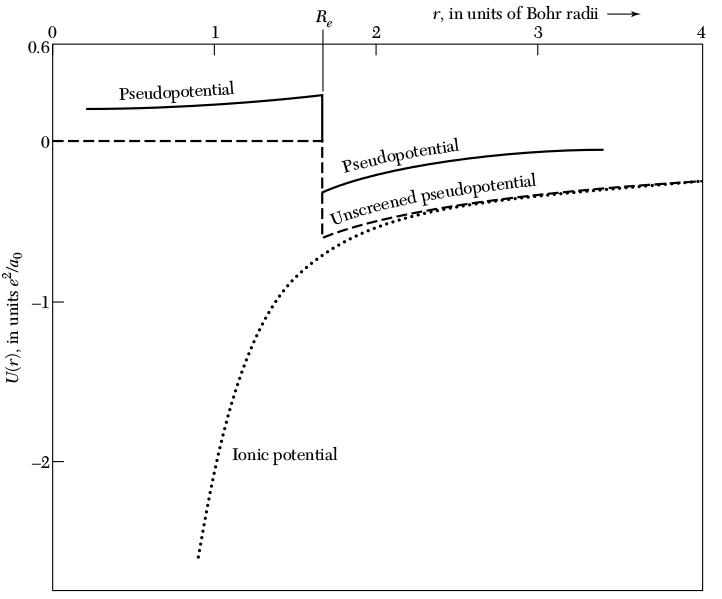
\includegraphics[height=1.60in,width=2.57in,viewport=0 0 980 600,clip]{Pseudo-model-empty_core.png}
\caption{\small \textrm{Pseudopotential for metallic sodium, based on the empty core model and screened by the Thomas-Fermi dielectric function.}}%(与文献\cite{EPJB33-47_2003}图1对比)
\label{Pseudo_model-empty_core}
\end{figure}
加入$\exp(a_4q^4)$因子使得可以适当选择$(a_4<0)$以保证这样赝势的Fourier展开很快收敛。常用半导体材料的赝势参数$a_i$可以从文献\cite{PRB15-2154_1977}得到。这种形式的赝势通常称为软芯(softcore)势。一般说,推导模型赝势要遵从如下三个原则:
\begin{enumerate}
  \item 
要避免引入有大的散射动量$q(q\gg 2k_F)$的平面波作基函数(会引起收敛困难);%与离子赝势在正空间不连续有关。
  \item 
要考虑到赝势的非局域效应;
  \item 
为确定势能参数,尽量使用与金属性质没有直接关联的实验数据。
\end{enumerate}
\begin{figure}[h!]
\centering
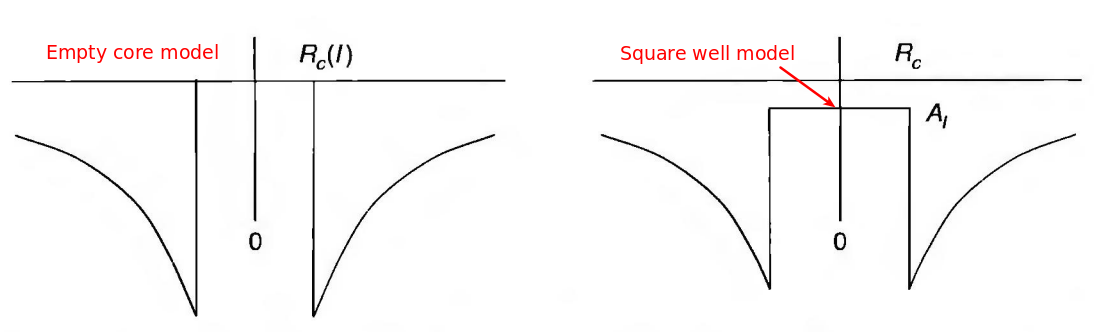
\includegraphics[height=1.30in,width=4.17in,viewport=0 0 1150 350,clip]{Pseudo-model.png}
\caption{\small \textrm{Left:``Empty core'' model potential of Ashcroft in which the potential is zero inside radius $R_c(l)$ which is different for each $l$. Right: Square well model potential with value $A_l$ inside a cut-off radius $R_c$, proposed by Abarenkov and Heine and fit to atomic data by Animalu and Heine..}}% The fact that the potential are weak, zero, or even positive inside cut-off radius $R_c$ is an illustration of the ``cancellation theorem''(与文献\cite{EPJB33-47_2003}图1对比)
\label{Pseudo-model}
\end{figure}

\subsection{模守恒赝势}
直接构造模型赝势是非常困难的,根据密度泛函理论,自洽的球形屏蔽势和与径向波函数构成Kohn-Sham方程的解,因此可以通过构造合理的赝波函数得到赝势:
\begin{equation}
  \left[-\frac12\frac{d^2}{dr^2}+\frac{l(l+1)}{2r^2}+V(\rho,r)\right]P_{nl}(r)=\varepsilon_{nl}P_{nl}
  \label{eq:solid-103}
\end{equation}
这里$V(\rho,r)$是自洽单电子势$$V(\rho,r)=-Z/r+V_H(\rho,r)+V_{xc}^{LDA}(\rho(r))$$
$V_H(\rho,r)$是Hartree势,$V_{xc}^{LDA}(\rho(r))$是LDA的交换-相关势。

这样得到的赝势称为第一原理赝势,赝势构造的重点由构造赝势本身转移到构造合适的赝波函数。目前使用的电子结构计算的主要赝势方法都是求解全电子波函数,构造相适应的赝函数,再通过径向方程\eqref{eq:solid-103}确定赝势。

绝大部分构造的第一原理赝势满足四个条件\cite{PRB12-4200_1975,PRB18-5449_1978,PRB19-568_1979,PRB20-4082_1979,PRB26-4199_1982,PRL43-1494_1979,JPC13-L189_1980,PRB32-8412_1985,PRB43-1993_1991}:
\begin{itemize}
	\item 首先,由赝势生成的价电子赝波函数不含节点;
	\item 其次,在截断半径$r_{cl}$之外\cite{JPC13-L189_1980,PRB43-1993_1991},具有相同角动量$l$的原子径向赝波函数(pseudo-potential, PP)与全电子波函数(all-electron, AE)相等,%即
\begin{equation}
  P_l^{PP}(r)=P_l^{AE}(r)\quad \mbox{满足}r>r_{cl}
  \label{eq:solid-104}
\end{equation}
或者快速收敛到该值\cite{PRB18-5449_1978,PRL43-1494_1979,PRB32-8412_1985};
	\item 第三,两种波函数在截断半径$r_{cl}$内包含的电荷密度相等\cite{PRL43-1494_1979,PRB43-1993_1991},
\begin{equation}
  \int_0^{r_{cl}}|P_l^{PP}(r)|^2dr=\int_0^{r_{cl}}|P_l^{AE}(r)|^2dr
  \label{eq:solid-105}
\end{equation}
	\item 最后,价态的全电子和赝势的本征值必须相等,$e_l^{PP}=e_l^{AE}$。满足上述全部条件的赝势一般称为模守恒赝势(norm-conserving pseudopotential, NCPP)\cite{PRL43-1494_1979}。有很多方法可以构造出满足上述条件的赝波函数\cite{PRB18-5449_1978,PRB26-4199_1982,PRL43-1494_1979,JPC13-L189_1980,PRB32-8412_1985,PRB43-1993_1991}。得到赝波函数后,逆向求解径向Schr\"odinger方程,可以得到屏蔽(src)赝势:
\begin{equation}
  V_{src,l}^{PP}=\varepsilon_l-\frac{l(l+1)}{2r^2}+\frac1{2P_l^{PP}(r)}\frac{d^2}{dr^2}P_l^{PP}(r)
  \label{eq:solid-106}
\end{equation}
从式\eqref{eq:solid-106}可见,因为赝波函数没有节点,赝势是平缓的,除了原子球心位置不再有其他奇点。
\end{itemize}
\begin{figure}[h!]
\centering
\vspace*{-0.10in}
\includegraphics[height=1.30in,width=4.17in,viewport=0 0 1150 350,clip]{Pseudo-OPW_NCPP.png}
\caption{\small \textrm{Schematic example of a valence function that has the character of a $3s$ orbital near the nucleus and two examples of smooth functions (dashed lines) that equal the full wave-function outside the core region.}}% Left: the smooth part of the valence function defined by OPW-like equation; Right: a smooth pseudo-function that satisfies the norm-conservation condition.(与文献\cite{EPJB33-47_2003}图1对比)
\label{Pseudo-OPW_NCPP}
\end{figure}
由价电子产生的屏蔽与其所处的环境有关,如果扣除价电子屏蔽效应可以得到离子赝势。在自洽迭代过程中利用离子赝势得到特定环境的电子屏蔽。从屏蔽赝势中减去根据赝波函数计算得到的Hartree赝势$V_H^{PP}(r)$和交换-相关赝势$V_{xc}^{PP}(r)$,即离子赝势\cite{PRB43-1993_1991}:
$$V_{ion,H}^{PP}(r)=V_{src,H}^{PP}(r)-V_H^{PP}(r)-V_{xc}^{PP}(r)$$
赝波函数的每个角动量分量有不同的势能,离子赝势算符可以写成:
\begin{equation}
  \hat V_{ion}^{PP}(r)=V_{ion,local}^{PP}+\sum_lV_{nonlocal,l}(r)\hat P_l
  \label{eq:solid-107}
\end{equation}
这里$V_{ion,local}^{PP}(r)$是局域势,$V_{nonlocal,l}(r)=V_{ion,l}^{PP}(r)-V_{ion,local}^{PP}(r)$是角动量$l$的非局域(或半局域)势。$\hat P_l$是投影算符,从波函数中投影出角动量的$l$分量。

Kleinman和Bylander(KB)\cite{PRL48-1425_1982}提出将半局域势\eqref{eq:solid-107}变换为非局域形式的过程:
$$V_{nonlocal,l}^{KB}=\dfrac{|V_{nonlocal,l}(r)\Phi_l^{PP,0}(r)\rangle\langle\Phi_l^{PP,0}(r)V_{nonlocal,l}(r)|}{\langle\Phi_l^{PP,0}(r)|V_{nonlocal,l}(r)|\Phi_l^{PP,0}(r)\rangle}$$
这里$V_{nonlocal,l}(r)$是半局域势[式\eqref{eq:solid-107}],$\Phi_l^{PP,0}(r)$是用以计算赝势的原子角动量$l$的参考赝波函数。选择特定的非局域表象,可以很大程度上节省计算时间。

\subsection{超软赝势}
赝势构造的模守恒条件很好地解决了赝势可移植性问题,但对$1s$、$2p$、$3d$等轨道,因为径向波函数本身没有节点,用模守恒方案获得的赝势过于“硬”,所需平面波基组依然非常大。\textrm{Vanderbilt}提出的超软\textrm{(Ultra-soft)}赝势\cite{PRB41-7892_1990},解除了模守恒约束,实现对$1s$、$2p$、$3d$为价电子元素的高效计算。
\begin{figure}[h!]
\centering
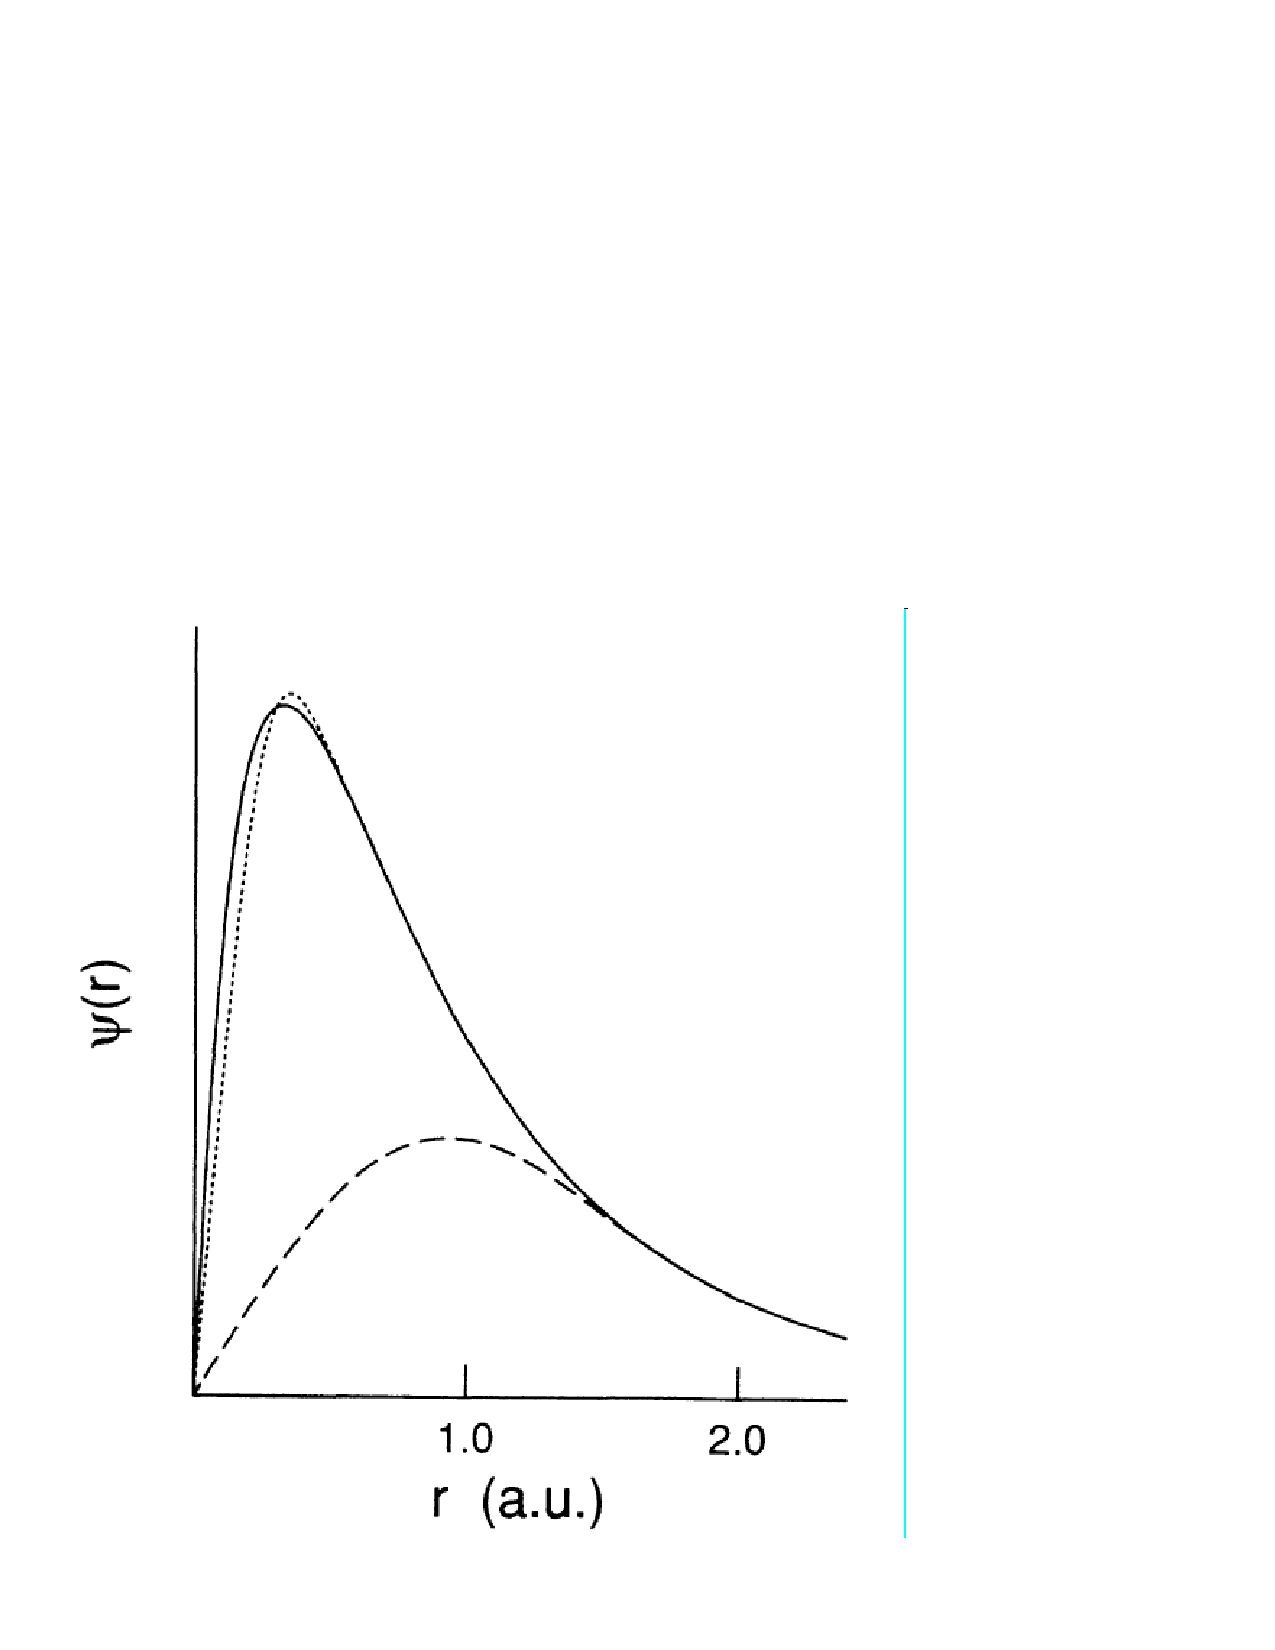
\includegraphics[height=1.35in,width=1.40in,viewport=30 55 415 500,clip]{Norm-US-wave.pdf}
\caption{\small \textrm{Oxygen 2} \textit{p} \textrm{radical wave function (solid), NC-pseudo-wave (dottde) and US-pseudo-wave (dashed).}}%(与文献\cite{EPJB33-47_2003}图1对比)
\label{Norm-US-wave}
\end{figure}

根据Vanderbilt的建议,对$1s$、$2p$、$3d$这种径向不包含节点的价电子波函数,构造赝波函数时放弃模守恒条件,只使用少量平面波基组,但是记录赝波函数与真实波函数的电荷密度差。\footnote{模守恒约束下,赝势\textrm{Schr\"odinger~}方程是标准本征值问题;放弃模守恒条件,引入电荷密度差,可将\textrm{Schr\"odinger}方程表示为广义本征值问题。}策略上,这是通过少量增加的电荷密度差计算为代价(以保持赝势的可移植性),换取基函数规模的大大减少。
\begin{equation}
	Q_{nm}(\vec r)=\varphi_n^{\ast}(\vec r)\varphi_m(\vec r)-\tilde\varphi_n^{\ast}(\vec r)\tilde\varphi_m(\vec r)
  \label{eq:uspp_4}
\end{equation}
超软赝势方法的实现:
\begin{enumerate}
	\item 在平缓的局域势函数$V^L(\vec r)$和赝波函数$|\phi_{lmj}(\vec r)\rangle$的基础上,构造辅助函数
\begin{equation}
	|\chi_{lmj}(\vec r)\rangle=\bigg[\varepsilon_{lj}-\dfrac12\nabla^2-V^L(\vec r)\bigg]|\phi_{lmj}(\vec r)\rangle
  \label{eq:uspp_1}
\end{equation}
	\item 引入矩阵$\mathbf{D}_{ij}=\langle\phi_i|\chi_j\rangle$和局域函数
\begin{equation}
	|\beta_i\rangle=\sum_j(\mathbf{D}^{-1})_{ji}|\chi_{j}\rangle
  \label{eq:uspp_2}
\end{equation}
	\item 与模守恒赝势类似,非局域赝势部分可由$\mathbf{D}$和$\beta_i$表示
\begin{equation}
	V_{NL}=\dfrac{|\chi_i\rangle\langle\chi_i|}{\langle\chi_i|\phi_i\rangle}=\sum_{i,j}\mathbf{D}_{ij}|\beta_i\rangle\langle\beta_j|
  \label{eq:uspp_3}
\end{equation}
\end{enumerate}
根据DFT的总能计算表达式
	\begin{equation}
		\begin{aligned}
			E_{\mathrm{total}}=&\sum_j^{\mathrm{occ}}\langle\phi_{lmj}|\bigg[-\dfrac12\nabla^2+V_{\mathrm{local}}^{\mathrm{ion}}+\sum_{s,s^{\prime}}\mathbf{D}_{s,s^{\prime}}^{\mathrm{ion}}|\beta_s\rangle\langle\beta_{s^{\prime}}|\bigg]|\phi_{lmj}\rangle\\
			&+E_{H}[n_v]+E_{N-N}+E_{XC}[n_v]
		\end{aligned}
  \label{eq:uspp_5}
	\end{equation}
其中$n_v(\vec r)=\sum\limits_j^{\mathrm{occ}}\phi_{lmj}^{\ast}(\vec r)\phi_{lmj}(\vec r)+\sum\limits_{s,s^{\prime}}\sum\limits_j^{\mathrm{occ}}\langle\phi_{lmj}|\beta_{s^{\prime}}\rangle\langle\beta_s|\phi_{lmj}\rangle Q_{s,s^{\prime}}(\vec r)$
	$$V_{\mathrm{local}}^{\mathrm{ion}}=V_{local}-V_{\mathrm H}-V_{XC}$$
	$$\mathbf{D}_{s,s^{\prime}}^{\mathrm{ion}}=\mathbf{D}_{s,s^{\prime}}-\int\mathrm{d}\vec r\big[V_{\mathrm{H}}(\vec r)+V_{XC}(\vec r)\big]Q_{s,s^{\prime}}(r)$$
可以得到广义本征值方程
	$$\bigg[-\dfrac12\nabla^2+V_{\mathrm{local}}+V_{NL}^{\mathrm{US}}-\varepsilon_i\bigg(\mathbf{1}+\sum_{s,s^{\prime}}Q_{s,s^{\prime}}|\beta_s\rangle\langle\beta_{s^{\prime}}|\bigg)\bigg]|\phi_{lmi}\rangle=0$$


\section{投影子缀加波(Projector Augmented Wave, PAW)方法}
PAW方法是\textrm{Bl\"ochl}于1994年独立提出来的一种计算方法\cite{PRB50-17953_1994},该方法的基本思想与OPW很相似,但同时结合了赝势方法和APW方法的优点,达到平衡计算效率和精度的目的。PAW方法刚提出来的时候并未引起注意,直到1999年\textrm{Kresse}指明了PAW方法和USPP方法的密切关联,USPP方法的计算程序只要经过简单改造就能扩展为PAW方法,有力地推动了PAW方法的广泛应用\cite{PRB59-1758_1999}。现在PAW方法已经成为最主要的可支持第一原理分子动力学(Ab initio Molecular Dynamics, AIMD)。

\subsection{PAW方法的基本思想}
与一般赝势方法不同,PAW方法的目标是全电子(all-electron)波函数\footnote{注意,“全电子”在\textrm{Bl\"ochl}原始文献\inlinecite{PRB50-17953_1994}中与“真实电子波函数”意义相近,强调电子在原子核附近的振荡行为,但并未严格区分价电子与芯电子;~而在\textrm{Kresse}的文献\inlinecite{PRB59-1758_1999}中则是明确指价电子波函数。%强调价电子波函数因与芯层电子正交而在原子核附近振荡;
此外,与“全电子”概念密切关联的是“全势(full-potential)”,两者在具体语境中有一定的区别,“全势”强调的是重现价电子感受到的势函数的效果。},体系中全部电子构成\textrm{Hilbert}空间,价电子与芯层态彼此正交,使得波函数在\textrm{Muffin-tin}球内振荡。
\textrm{Bl\"ochl}假设全电子波函数$|\Psi\rangle$与赝波函数$|\tilde\Psi\rangle$满足线性变换,即满足:
\begin{equation}
	|\Psi\rangle=\mathbf{\tau|}\tilde\Psi\rangle
	\label{eq:PAW-Blochl-01}
\end{equation}
%	$$\tau=\mathbf{1}+\sum_{\mathrm R}\hat\tau_{\mathrm R}$$
在原子核附近的$r_c$范围内\footnote{习惯上这个区域称为缀加区(\textrm{Augmentation region}).},除了平面波,还引入原子分波函数展开来表示波函数:
\begin{equation}
	|\Psi\rangle=|\tilde\Psi\rangle+\sum_i(|\phi_i\rangle-|\tilde\phi_i\rangle)\langle\tilde p_i|\tilde\Psi\rangle
	\label{eq:PAW-Blochl-02}
\end{equation}
在$r_c$外$|\tilde\Psi\rangle$与$|\Psi\rangle$变换前后保持不变,因此线性变换$\mathbf{\tau}$可表示为:
\begin{equation}
	\mathbf{\tau}=\mathbf{1}+\sum_i(|\phi_i\rangle-|\tilde\phi_i\rangle)\langle\tilde p_i|
	\label{eq:PAW-Blochl-03}
\end{equation}
其中$|\tilde p_i\rangle$是\textrm{MT}球内的投影函数,$i$表示原子位置$\vec R$、原子轨道($l,m$)和能级$\epsilon_k$的指标。\textrm{PAW}的波函数与赝波函数的关系,可以用图\ref{PAW_basic}表示。
\begin{figure}[h!]
\centering
\includegraphics[height=2.35in,width=4.1in,viewport=0 0 1280 745,clip]{PAW-baseset.png}
%\includegraphics[height=1.8in,width=4.in,viewport=30 210 570 440,clip]{PAW_projector.eps}
\caption{\small \textrm{The analysis of PAW basic function.}}%(与文献\cite{EPJB33-47_2003}图1对比)
\label{PAW_basic}
\end{figure}

\subsection{PAW表示下的能量表示与补偿电荷}
\textrm{PAW}方法通过投影算符和赝波函数实现全电子波函数计算,因此完整的\textrm{PAW}方法下,一般算符的期望值计算为
\begin{equation}
	\langle A \rangle=\langle\Psi|\mathbf{A}|\Psi\rangle=\langle\tilde\Psi|\mathbf{\tau}^{\dag}\mathbf{A}\mathbf{\tau}|\tilde\Psi\rangle=\langle\tilde\Psi|\tilde{\mathrm{A}}|\tilde\Psi\rangle
	\label{eq:PAW-Blochl-04}
\end{equation}
式中将$\mathrm{\tau}$用式\eqref{eq:PAW-Blochl-03}展开,因此赝算符$\tilde A$可表示为
\begin{equation}
	\tilde A=\mathbf{A}+\sum_i|\tilde p_i\rangle(\langle\phi_i|\mathbf{A}|\phi_i\rangle-\langle\tilde\phi_i|\mathbf{A}|\tilde\phi_i\rangle)\langle\tilde p_i|
	\label{eq:PAW-Blochl-05}
\end{equation}
%不难看出,赝重叠算符$\tilde O$可展开为
%\begin{equation}
%	\tilde O=\mathbf{1}+\sum_i|\tilde p_i\rangle(\langle\phi_i|\phi_i\rangle-\langle\tilde\phi_i|\tilde\phi_i\rangle)\langle\tilde p_i|
%	\label{eq:PAW-Blochl-06}
%\end{equation}
实空间中,电荷密度的算符为$|r\rangle\langle r|$,根据式\eqref{eq:PAW-Blochl-03},则电荷密度的计算
\begin{equation}
	n(\vec r)=\tilde n(\vec r)+n^1(\vec r)-\tilde n^1(\vec r)
	\label{eq:PAW-Blochl-07}
\end{equation}
这里
\begin{displaymath}
	\begin{aligned}
		\tilde n(\vec r)=&\sum_nf_n\langle\tilde\Psi_n|\vec r\rangle\langle\vec r|\tilde\Psi_n\rangle \\
n^1(\vec r)=&\sum_{n,(i,j)}f_n\langle\tilde\Psi_n|\tilde p_i\rangle\langle\phi_i|\vec r\rangle\langle\vec r|\phi_j\rangle\langle\tilde p_j|\tilde\Psi_n\rangle \\
\tilde n^1(\vec r)=&\sum_{n,(i,j)}f_n\langle\tilde\Psi_n|\tilde p_i\rangle\langle\tilde\phi_i|\vec r\rangle\langle\vec r|\tilde\phi_j\rangle\langle\tilde p_j|\tilde\Psi_n\rangle
	\end{aligned}
\end{displaymath}
$f_n$是占据态的电子数。注意,这里的$n^1$和$\tilde n^1$中包含了芯层电荷的贡献,即$\sum_n\langle\phi_n^c|\vec r\rangle\langle\vec r|\phi_n^c\rangle$,$\sum_n\langle\tilde\phi_n^c|\vec r\rangle\langle\vec r|\tilde\phi_n^c\rangle$和$\sum_n\langle\tilde\Psi_n^c|\vec r\rangle\langle\vec r|\tilde\Psi_n^c\rangle$。但是实际应用中,一般都是直接构造芯层态电荷密度,并不考虑芯层态波函数。

类似地,根据\textrm{DFT}理论,体系总能量泛函可以表示为
\begin{equation}
	\begin{aligned}
		E&=\sum_nf_n\langle\Psi_n|-\dfrac12\nabla^2|\Psi_n\rangle\\
		 &+\dfrac12\int\mathrm{d}\vec r\int\mathrm{d}\vec r^{\prime}\dfrac{(n+n^Z)(n+n^Z)}{|\vec r-\vec r^{\prime}|}+\int\mathrm{d}\vec r n\epsilon_{\mathrm{XC}}(n)
	\end{aligned}
	\label{eq:PAW-Blochl-08}
\end{equation}
在\textrm{PAW}框架下,总能可分解为$E=\tilde E+E^1-\tilde E^1$,每一项分别表示为:
\begin{equation}
	\begin{aligned}
		\tilde E&=\sum_nf_n\langle\tilde\Psi_n|-\dfrac12\nabla^2|\tilde\Psi_n\rangle\\
		 &+\dfrac12\int\mathrm{d}\vec r\int\mathrm{d}\vec r^{\prime}\dfrac{(\tilde n+\hat n)(\tilde n+\hat n)}{|\vec r-\vec r^{\prime}|}+\int\mathrm{d}\vec r \tilde n\bar v+\int\mathrm{d}\vec r \tilde n\epsilon_{\mathrm{XC}}(\tilde n)
 	\end{aligned}
	\label{eq:PAW-Blochl-09}
\end{equation}
\begin{equation}
	\begin{aligned}
		E^1&=\sum_{n,(i,j)}f_n\langle\tilde\Psi_n|\tilde p_i\rangle\langle\phi_i|-\dfrac12\nabla^2|\phi_j\rangle\langle\tilde p_j|\tilde\Psi_n\rangle\\
		 &+\dfrac12\int\mathrm{d}\vec r\int\mathrm{d}\vec r^{\prime}\dfrac{(n^1+n^Z)(n^1+n^Z)}{|\vec r-\vec r^{\prime}|}+\int\mathrm{d}\vec r n^1\epsilon_{\mathrm{XC}}(n^1)
 	\end{aligned}
	\label{eq:PAW-Blochl-10}
\end{equation}
\begin{equation}
	\begin{aligned}
		\tilde E^1&=\sum_{n,(i,j)}f_n\langle\tilde\Psi_n|\tilde p_i\rangle\langle\tilde\phi_i|-\dfrac12\nabla^2|\tilde\phi_j\rangle\langle\tilde p_j|\tilde\Psi_n\rangle\\
		 &+\dfrac12\int\mathrm{d}\vec r\int\mathrm{d}\vec r^{\prime}\dfrac{(\tilde n^1+\hat n)(\tilde n^1+\hat n)}{|\vec r-\vec r^{\prime}|}+\int\mathrm{d}\vec r \tilde n^1\bar v+\int\mathrm{d}\vec r \tilde n^1\epsilon_{\mathrm{XC}}(\tilde n^1)
 	\end{aligned}
	\label{eq:PAW-Blochl-11}
\end{equation}
式\eqref{eq:PAW-Blochl-09}和\eqref{eq:PAW-Blochl-11}中$\bar v$是缀加区内的任意局域函数,只要该区域内满足条件$\tilde n=\tilde n^1$,则$\bar v$对总能量的贡献为0。与赝势方法类似,$\bar v$取去屏蔽局域赝势。

类似地,式\eqref{eq:PAW-Blochl-09}和\eqref{eq:PAW-Blochl-11}中$\hat n$为补偿电荷,取值范围限于缀加区。与超软赝势中的补偿电荷的要求类似,\textrm{PAW}方法中的$\hat n$存在使得电荷密度$(n^1+n^Z)$和$(\tilde n^1+\hat n)$在缀加区外的多极矩贡献相等,因此不必再考虑电荷在缀加区外的相互作用,只需考虑$\hat n$在$\tilde E$中的贡献。$\hat n$可表示为单个原子截断区间的补偿电荷之和,即$\hat n=\sum_R\hat n_R$,并且$\hat n_R(r)$可用\textrm{Gaussian}函数展开,即
\begin{equation}
	\hat n_R(r)=\sum_{L=(l,m)}g_{RL}(r)Q_{RL}
	\label{eq:PAW-Blochl-12}
\end{equation}
式中$g_{RL}(r)$是广义的\textrm{Gaussian}函数,表示如下
	$$g_{RL}(r)=C_l|r-R|^lY_L(r-R)\mathrm{e}^{-(|r-R|/r_c)^2}$$
其系数$C_l$是归一化系数,由条件
	$\int\mathrm{d}rr^lY_L(r)g_L(r)=1$
确定。
式\eqref{eq:PAW-Blochl-12}的$Q_{RL}$由构造补偿电荷所须满足的多极矩条件确定
	$$Q_{RL}=\int\mathrm{d}r|r-R|^l\big[n_R^1(r)+n_R^Z(r)-\tilde n_R^1(r)\big]Y_L^{\ast}(r-R)$$

一般来说,原子的补偿电荷的\textrm{Gaussian}展开在缀加区会快速衰减,这意味着最终需要很高的平面波来展开。在\textrm{Bl\"ochl}的方案中,建议引入新的补偿电荷$\hat n^{\prime}$,满足条件:~\footnote{这是\textrm{Bl\"ochl}方案与后来\textrm{Kresse}方案处理补偿电荷的主要区别。}
	\begin{itemize}
		\item $\hat n^{\prime}$与$\hat n$具有相同的多极矩(保留原来的补偿电荷的基本要求)
		\item $\hat n^{\prime}$的\textrm{Gaussian}函数展开的衰减半径$r_c^{\prime}$比$r_c$大得多,可以用很少的平面波展开
	\end{itemize}
因此,能量$\tilde E$中的静电相互作用可以表示为
	\begin{equation}
		\begin{aligned}
			&\dfrac12\int\mathrm{d}r\int\mathrm{d}r^{\prime}\dfrac{(\tilde n+\hat n)(\tilde n+\hat n)}{|r-r^{\prime}|}\\
			=&\underline{\dfrac12\int\mathrm{d}r\int\mathrm{d}r^{\prime}\dfrac{(\tilde n+\hat n^{\prime})(\tilde n+\hat n^{\prime})}{|r-r^{\prime}|}}
			+\underline{\int\mathrm{d}r\tilde n(r)\hat v(r)}+\underline{\sum_{R,R^{\prime}}U_{R,R^{\prime}}}
		\end{aligned}
		\label{eq:PAW-Blochl-13}
	\end{equation}
其中第一项是平滑函数,可以在\textrm{Fourier}空间计算
	$$2\pi V\sum_G\dfrac{|\tilde n(G)+\hat n^{\prime}(G)|^2}{G^2}$$
第二项的$\hat v(r)$表示为
	$$\hat v(r)=\int\mathrm{d}r^{\prime}\dfrac{\hat n(r^{\prime})-\hat n^{\prime}(r^{\prime})}{|r-r^{\prime}|}$$
虽然$\hat v(r)$和$n(r)$一样有高\textrm{Fourier}截断,但因为$\tilde n(G)$只需要少量平面波展开,所以$\hat v(r)$的高阶部分不会对$\int\mathrm{d}r\tilde n(r)\hat v(r)$有贡献。最后一项中$U_{R,R^{\prime}}$是原子间的短程成对势
	$$U_{R,R^{\prime}}=\dfrac12\int\mathrm{d}r\int\mathrm{d}r^{\prime}\dfrac{\hat n_R(r)\hat n_{R^{\prime}}(r^{\prime})-\hat n_R^{\prime}(r)\hat n_{R^{\prime}}^{\prime}(r^{\prime})}{|r-r^{\prime}|}$$
这一项可以通过\textrm{Ewald}求和方法计算。

\subsection{PAW方法的Kohn-Sham方程与原子分波、投影函数}
在\textrm{DFT}框架下,应用\textrm{PAW}方法,除了总能量的表示外,还要考虑\textrm{Kohn-Sham}方程。根据式\eqref{eq:PAW-Blochl-05},平面波基表示的重叠算符可以写成:
\begin{equation}
	\tilde O=\mathbf{1}+\sum_{i,j}|\tilde p_i\rangle\bigg[\langle\phi_i|\phi_j\rangle-\langle\tilde\phi_i|\tilde\phi_j\rangle\bigg]\langle\tilde p_j|
	\label{eq:PAW-Blochl-14}
\end{equation}
类似地,可以得到根据定义,经典的\textrm{DFT}中\textrm{Hamilitonian}算符:%\cite{PRB50-17953_1994}
\begin{equation}
	\begin{aligned}
		\dfrac{\mathrm{d}E}{\mathrm{d}\rho}=&\dfrac{\partial\mathrm{Tr}[-\frac12\nabla^2\rho]}{\partial\rho}+\int\mathrm{d}r\dfrac{\partial E}{\partial n(r)}\dfrac{\mathrm{Tr}[|r\rangle\langle r|\rho]}{\partial\rho}\\
		=&-\dfrac12\nabla^2+v
	\end{aligned}
	\label{eq:PAW-DFT-H}
\end{equation}
这里$v(r)=|r\rangle\dfrac{\partial E}{\partial n(r)}\langle r|$。\textrm{PAW}方法中,\textrm{Hamiltonian}算符是总能量对赝电荷密度$\tilde\rho=\sum\limits_i|\tilde\Psi_n\rangle f_n\langle\tilde\Psi_n|$的变分(约束条件是$\langle\tilde\Psi_n|\tilde O|\tilde\Psi_m\rangle=\delta_{nm}$):
\begin{equation}
	\begin{aligned}
		\dfrac{\mathrm{d}E}{\mathrm{d}v\tilde\rho}=&\dfrac{\partial\mathrm{Tr}[-\frac12\nabla^2\rho]}{\partial\rho}+\int\mathrm{d}r\dfrac{\partial E}{\partial n(r)}\dfrac{\mathrm{Tr}[|r\rangle\langle r|\rho]}{\partial\rho}\\
		=&-\dfrac12\nabla^2+v
	\end{aligned}
	\label{eq:PAW-Blochl-H}
\end{equation}
注意,这里势能是$\tilde n$、$\tilde n^1$、$\tilde n^1$和多极矩$Q_{\mathrm{RL}}$的函数,因此可得
\begin{equation}
	\begin{aligned}
		\dfrac{\mathrm{d}E}{\mathrm{d}\tilde\rho}=&\dfrac{\partial\mathrm{Tr}[\tilde\rho\tilde T]}{\partial\rho}+\int\mathrm{d}r\dfrac{\partial E}{\partial n(r)}\dfrac{\partial\tilde n}{\partial\rho}\\
		&+\int\mathrm{d}r\bigg(\dfrac{\partial E}{\partial n^1}+\sum_{\mathrm{R,L}}\dfrac{\partial E}{\partial Q_{\mathrm{RL}}}\dfrac{\partial Q_{\mathrm{RL}}}{\partial n^1}\bigg)\dfrac{\partial n^1}{\partial\rho}\\
		&+\int\mathrm{d}r\bigg(\dfrac{\partial E}{\partial\tilde n^1}+\sum_{\mathrm{R,L}}\dfrac{\partial E}{\partial Q_{\mathrm{RL}}}\dfrac{\partial Q_{\mathrm{RL}}}{\partial\tilde n^1}\bigg)\dfrac{\partial\tilde n^1}{\partial\rho} 
	\end{aligned}
	\label{eq:PAW-Blochl-H-n}
\end{equation}
式\eqref{eq:PAW-Blochl-H-n}中动能算符$\tilde T$的定义为:~
		\begin{equation}
			\tilde T=-\dfrac12\nabla^2+\sum_{i,j}|\tilde p_i\rangle[\langle\phi_i|-\dfrac12\nabla^2|\phi_j\rangle-\langle\tilde\phi_i|-\dfrac12\nabla^2|\tilde\phi_j\rangle]\langle\tilde p_j|
			\label{eq:PAW-Blochl-T}
		\end{equation}
式\eqref{eq:PAW-Blochl-H-n}中对赝电荷密度求导的项为:~
\begin{equation}
	\begin{aligned}
		\tilde v(r)=\dfrac{\partial E}{\partial\tilde n(r)}=&\int\mathrm{d}r^{\prime}\dfrac{\tilde n(r^{\prime})+\hat n^{\prime}(r^{\prime})}{|r-r^{\prime}|}\\
		&+\hat v(r)+\bar v(r)+\mu_{\mathrm{XC}}[\tilde n(r)]
	\end{aligned}
	\label{eq:PAW-Blochl-v}
\end{equation}
式\eqref{eq:PAW-Blochl-H-n}中对多极矩的求导,注意到多极矩是通过补偿电荷$\hat n$和$\hat n^{\prime}$进入总能量的表达式,因此有:~
\begin{displaymath}
	\begin{aligned}
		\dfrac{\partial E}{\partial Q_{\mathrm{RL}}}=&\int\mathrm{d}r\dfrac{\partial E}{\partial \hat n(r)}\dfrac{\partial\hat n(r)}{\partial Q_{\mathrm{RL}}}+\int\mathrm{d}r\dfrac{\partial E}{\partial \hat n^{\prime}(r)}\dfrac{\partial\hat n^{\prime}(r)}{\partial Q_{\mathrm{RL}}}\\
		=&\int_{\mathrm M}\mathrm{d}r\int_{\mathrm M}\mathrm{d}r^{\prime}\dfrac{g_{\mathrm{RL}}(r)\tilde n(r^{\prime})+g_{\mathrm{RL}}^{\prime}(r)\hat n^{\prime}(r^{\prime})}{|r-r^{\prime}|}\\
		=&\int_{\mathrm A}\mathrm{d}r\int_{\mathrm A}\mathrm{d}r^{\prime}\dfrac{g_{\mathrm{RL}}(r)\tilde n(r^{\prime})+g_{\mathrm{RL}}^{\prime}(r)\hat n^{\prime}(r^{\prime})}{|r-r^{\prime}|}\\
		=&\int_{\mathrm{RG}}\mathrm{d}r\int_{\mathrm{RG}}\mathrm{d}r^{\prime}\dfrac{g_{\mathrm{RL}}(r)\tilde n(r^{\prime})+g_{\mathrm{RL}}^{\prime}(r)\hat n^{\prime}(r^{\prime})}{|r-r^{\prime}|}
	\end{aligned}
\end{displaymath}
这里积分域$\mathrm{M}$表示平面波网格点(\textrm{Fourier}网格点),$\mathrm{RG}$表示径向网格点,$\mathrm{A}$表示解析积分(或\textrm{Ewald}求和),因此可有
\begin{equation}
	\begin{aligned}
		v_{\mathrm R}^0(r)=&\sum_{\mathrm L}\dfrac{\partial E}{\partial Q_{\mathrm{RL}}}\dfrac{\partial Q_{\mathrm{RL}}}{\partial n^1(r)}=-\sum_{\mathrm L}\dfrac{\partial E}{\partial Q_{\mathrm{RL}}}\dfrac{\partial Q_{\mathrm{RL}}}{\partial\tilde n^1(r)}\\
		=&\sum_{\mathrm L}(r-R)^lY_L^{\ast}(|r-R|)\dfrac{\partial E}{\partial Q_{\mathrm{RL}}}
	\end{aligned}
	\label{eq:PAW-Blochl-v_R}
\end{equation}
\begin{equation}
	\begin{aligned}
		v_{\mathrm R}^1(r)=&\dfrac{\partial E}{\partial n^1(r)}+\sum_{\mathrm L}\dfrac{\partial E}{\partial Q_{\mathrm{RL}}}\dfrac{\partial Q_{\mathrm{RL}}}{\partial n^1(r)}\\
		=&\int_{\mathrm R}\mathrm{d}r^{\prime}\dfrac{n_{\mathrm R}^1(r^{\prime})+n_{\mathrm R}^Z(r^{\prime})}{|r-r^{\prime}|}+\mu_{\mathrm{XC}}[n_{\mathrm R}^1(r)]+v_{\mathrm R}^0(r)
	\end{aligned}
	\label{eq:PAW-Blochl-v1_R}
\end{equation}
\begin{equation}
	\begin{aligned}
		\tilde v_{\mathrm R}^1(r)=&\bigg(\dfrac{\partial E}{\partial\tilde n^1(r)}+\sum_{\mathrm L}\dfrac{\partial E}{\partial Q_{\mathrm{RL}}}\dfrac{\partial Q_{\mathrm{RL}}}{\tilde n^1(r)})\\
		=&\int_{\mathrm R}\mathrm{d}r^{\prime}\dfrac{\tilde n_{\mathrm R}^1(r^{\prime})+\hat n_{\mathrm R}(r^{\prime})}{|r-r^{\prime}|}+\mu_{\mathrm{XC}}[\tilde n_{\mathrm R}^1(r)]+v_{\mathrm R}^0(r)
	\end{aligned}
	\label{eq:PAW-Blochl-tv1_R}
\end{equation}
综上,\textrm{Hamilton}算符:
\begin{equation}
	\begin{aligned}
		\tilde H=&-\dfrac12\nabla^2+\tilde v+\sum_{i,j}|\tilde p_i\rangle\bigg[\langle\phi_i|-\dfrac12\nabla^2+v^1|\phi_j\rangle\\
			&-\langle\tilde\phi_i|-\dfrac12\nabla^2+\tilde v^1|\tilde\phi_j\rangle\bigg]\langle\tilde p_j| 
	\end{aligned}
	\label{eq:PAW-Blochl-15}
\end{equation}
在\textrm{PAW}方法中,完整的势函数\textrm{(full potential)}算符表示为:
\begin{equation}
	v(\vec r)=\tilde v(\vec r)+v^1(\vec r)-\tilde v^1(\vec r)
	\label{eq:PAW-Blochl-16}
\end{equation}
与电荷密度的表示类似,势函数是由平滑的平面波表示赝势函数$\tilde v$和位于每个原子缀加区的单中心局域的原子势$v^1$和$\tilde v^1$叠加而成。平滑势可用平面波展开,而原子势则表示成径向函数和角度部分乘积。

总能量泛函对赝波函数求导,可有
\begin{equation}
	\left.\dfrac{\partial E[\tilde\Psi, R]}{\partial\langle\tilde\Psi_n|}\right|_R=\tilde H|\tilde\Psi_n\rangle f_n
	\label{eq:PAW-Blochl-17}
\end{equation}

\textrm{PAW}方法除了采用平面波作为基函数,在每个原子核附近$r_c$范围内的缀加区,还保留了原子波函数和以平面波表示的赝波函数,它们构成\textrm{PAW}方法的基函数的一部分,%在\textrm{PAW}方法中,将与原子分波展开所有相关的数据统称原子数据集(data set),
也是\textrm{PAW}计算的基础。

\textrm{PAW}与原子分波展开所有相关的数据主要包括:~
	\begin{itemize}
		\item 原子分波信息:~原子分波函数$\phi_i$、赝分波函数$\tilde\phi_i$和投影波函数$p_i$
		\item 电荷密度信息:~$r_c$内的电荷密度$n^1$、赝电荷密度$\tilde n^1$和补充电荷$\hat n$
		\item 赝势信息:~原子局域赝势$\tilde v_{\mathrm{loc}}(\vec r)$
	\end{itemize}
\textrm{PAW}方法的原子分波与赝势方法相似,一套原子数据集将用于各种化学环境下的\textrm{PAW}计算,即要求原子数据集有良好的可移植性;~与赝势方法不同之处在于\textrm{PAW}原子集中除了赝原子的信息,还包含了真实原子的信息。

原子分波函数由原子\textrm{Schr\"odinger}方程确定
\begin{equation}
	\bigg(-\dfrac12\nabla^2+v_{at}-\varepsilon_i^1\bigg)|\phi_i\rangle=0
	\label{eq:PAW-Blochl-18}
\end{equation}
根据\textrm{Bl\"ochl}的建议,为确定分波函数$\phi_i$,一般通过适当选择$\varepsilon_i^1$(原子价电子能量附近),并要求在缀加区与芯层分波函数正交。实际应用中,还可以类似\textrm{LAPW}方法,对每个分波引入多个(一般是两个)分波函数。

对于赝原子分波,\textrm{Bl\"ochl}建议的赝化方案与传统赝势构造类似\cite{PRL43-1494_1979,PRB26-4119_1982,PRB40-2980_1989}:
通过引入局域赝势:%$$w_i(r)=\tilde v_{at}(r)+c_ik(r)=\tilde v_{at}(0)\mathrm{e}^{-(r/r_k)^{\lambda}}+[1-k(r)]v_{at}(r)+c_i\mathrm{e}^{-(r/r_k)^{\lambda}}$$
\begin{equation}
	w_i(r)=\tilde v_{\mathrm{at}}(0)\mathrm{e}^{-(r/r_k)^{\lambda}}+[1-\mathrm{e}^{-(r/r_k)^{\lambda}}]v_{\mathrm{at}}(r)+c_i\mathrm{e}^{-(r/r_k)^{\lambda}}
	\label{eq:PAW-Blochl-19}
\end{equation}
其中$\tilde v_{\mathrm{at}}$是用多项式近似的原子赝势,参数$r_k$和$\lambda$由条件在$r_c$外赝势与原子势相等确定。赝分波函数由方程
\begin{equation}
	\bigg(-\dfrac12\nabla^2+w_i(r)-\varepsilon_i^1\bigg)|\tilde\phi_i\rangle=0
	\label{eq:PAW-Blochl-20}
\end{equation}
确定。式\eqref{eq:PAW-Blochl-19}的系数$c_i$根据赝分波函数$\tilde\phi_i$与分波函数$\phi_i$在$r_c$外相等确定。
\begin{figure}[h!]
\centering
\includegraphics[height=2.6in,width=3.2in,viewport=0 0 570 545,clip]{PAW-partical.png}
\caption{\small \textrm{The partical-wave of Fe atom.}}%(与文献\cite{EPJB33-47_2003}图1对比)
\label{PAW_partical_Fe}
\end{figure}

按照\textrm{Bl\"ochl}建议的投影函数的构造方案,初始形式与超软赝势的辅助函数计算类似:
\begin{equation}
	|\tilde p_i\rangle=\bigg(-\dfrac12\nabla^2+\tilde v_{at}-\varepsilon_i^1\bigg)|\tilde\phi_i\rangle
	\label{eq:PAW-Blochl-21}
\end{equation}
考虑到投影函数与赝分波函数的正交性$\langle\tilde p_i|\tilde\phi_j\rangle=\delta_{ij}$,对于给定下标的投影函数$\tilde p_i$,要求与所有$j<i$的赝分波函数正交,因此\textrm{Bl\"ochl}采用\textrm{Gram-Schmidt}正交化方法,得到正交的投影函数
$$|\tilde p_i\rangle=|\tilde p_i\rangle-\sum_{j=1}^{i-1}|\tilde p_j\rangle\langle\tilde\phi_j|\tilde p_i\rangle$$
%	$$|\phi_i\rangle=|\phi_i\rangle-\sum_{j=1}^{i-1}|\phi_j\rangle\langle\tilde p_j|\tilde\phi_i\rangle$$
%	$$|\tilde\phi_i\rangle=|\tilde\phi_i\rangle-\sum_{j=1}^{i-1}|\tilde\phi_j\rangle\langle\tilde p_j|\tilde\phi_i\rangle$$
在此基础上,分波函数与赝分波函数也分别与投影函数正交
$$|\phi_i\rangle=|\phi_i\rangle-\sum\limits_{j=1}^{i-1}|\phi_j\rangle\langle\tilde p_j|\tilde\phi_i\rangle$$
$$|\tilde\phi_i\rangle=|\tilde\phi_i\rangle-\sum\limits_{j=1}^{i-1}|\tilde\phi_j\rangle\langle\tilde p_j|\tilde\phi_i\rangle$$
最终作为基函数的$\phi_i$、$\tilde\phi_i$、$\tilde p_i$是通过迭代得到的。
%\begin{figure}[h!]
%\centering
%\vspace*{-0.4in}
%\includegraphics[height=1.5in,width=2.3in,viewport=0 0 1100 745,clip]{PAW_projector-2.png}
%\caption{\small \textrm{The projector of PAW.}}%(与文献\cite{EPJB33-47_2003}图1对比)
%\label{PAW_projector}
%\end{figure}
%\begin{itemize}
%	\item 与分波具有相同的角动量$l$
%	\item 局域在缀加区域(Augmentation region)
%	\item 节点依次增加
%\end{itemize}

与赝势的去屏蔽过程类似,%在得到赝势$\tilde v_{\mathrm{at}}$的基础上,可以计算
缀加区的局域势表示形式为:
\begin{equation}
	\bar v(r)=\tilde v_{at}(r)-\int\mathrm{d}r^{\prime}\dfrac{\tilde n(r^{\prime})+\hat n(r^{\prime})}{|r-r^{\prime}|}-\mu_{xc}[\tilde n(r)]
	\label{eq:PAW-Blochl-22}
\end{equation}
注意到在缀加区,式\eqref{eq:PAW-Blochl-22}由束缚态计算得到,计算电子的\textrm{Coulomb}相互作用、交换-相关势的贡献时,赝电荷密度$\tilde n(r)$包括赝芯电荷密度$\tilde n^c$和赝价电子密度。其中赝芯电荷的构造与赝势方法相同,价电子密度来自束缚态赝分波函数$|\tilde\Psi_j\rangle$,它由方程\cite{PRB50-17953_1994}
%中的赝电荷密度$\tilde n(r)$由赝分波波函数$|\tilde\Psi_j\rangle$确定。对于束缚态,
\begin{equation}
	\bigg[-\dfrac12\nabla^2+\tilde v_{at}-\varepsilon+\sum_{(i,j)}|\tilde p_i\rangle\big(\mathrm{d}H_{ij}-\varepsilon\mathrm{d}O_{ij}\big)\langle\tilde p_j|\bigg]|\tilde\Psi_j\rangle=0
	\label{eq:PAW-Blochl-23}
\end{equation}
确定,式\eqref{eq:PAW-Blochl-23}中$\mathrm{d}H_{ij}$和$\mathrm{d}O_{ij}$分别是
$$\mathrm{d}H_{ij}=\langle\phi_i|-\dfrac12\nabla^2+v_{at}|\phi_j\rangle-\langle\tilde\phi_i|-\dfrac12\nabla^2+\tilde v_{at}|\tilde\phi_j\rangle$$
$$\mathrm{d}O_{ij}=\langle\phi_i|\phi_j\rangle-\langle\tilde\phi_i|\tilde\phi_j\rangle$$
式\eqref{eq:PAW-Blochl-23}的求解,参见文献\inlinecite{PRB50-17953_1994}。

上述讨论不难看出,\textrm{PAW}方法的原子信息计算与赝势方法很相似,其中包括
\begin{itemize}
	\item 缀加局域区截断半径$r_c$
	\item 芯电荷密度$n^c$和赝芯电荷密度$\tilde n^c$
	\item (价)电子分波函数$|\phi_i\rangle$和赝分波函数$|\tilde\phi_i\rangle$
	\item 矩阵元$\langle\phi_i|-\dfrac12\nabla^2|\phi_j\rangle-\langle\tilde\phi_i|-\dfrac12\nabla^2|\tilde\phi_j\rangle$和$\langle\phi_i|\phi_j\rangle-\langle\tilde\phi_i|\tilde\phi_j\rangle$
\end{itemize}
%如果解$$|\tilde\Psi\rangle=|u\rangle+\sum_i|w_i\rangle c_i$$
%其中$|u\rangle$和$|w_i\rangle$的定义分别为
%$$\big(-\frac12\nabla^2+\tilde v-\varepsilon\big)|u\rangle=0$$
%$$\big(-\frac12\nabla^2+\tilde v-\varepsilon\big)|w_i\rangle=|\tilde p_i\rangle$$
%因此可以得到
%$$c_i=-\sum_{j,l}\bigg[\delta_{ij}+\sum_k\mathrm{d}H_{ik}-\varepsilon\mathrm{d}O_{ik}\langle\tilde p_k|w_j\rangle\bigg]^{-1}\big(\mathrm{d}H_{jl}-\varepsilon\mathrm{d}O_{jl}\big)\langle p_l|u\rangle$$

%\frame
%{
%%	\frametitle{\textrm{PAW}原子数据集}
%	\frametitle{\textrm{PAW Augmentation}}
%\begin{figure}[h!]
%\centering
%\includegraphics[height=2.3in,width=4.0in,viewport=0 0 1280 745,clip]{Figures/PAW-baseset.png}
%\caption{\small \textrm{The Augmentation of PAW.}}%(与文献\cite{EPJB33-47_2003}图1对比)
%\label{PAW_baiseset}
%\end{figure}
%}

%\frame
%{
%	\frametitle{\textrm{PAW Augmentation}}
%\begin{figure}[h!]
%\centering
%\includegraphics[height=2.3in,width=4.0in,viewport=0 0 1100 745,clip]{Figures/PAW-projector.png}
%\caption{\small \textrm{The projector of PAW.}}%(与文献\cite{EPJB33-47_2003}图1对比)
%\label{PAW_projector}
%\end{figure}
%}

\subsection{\rm{PAW}方法与\rm{USPP}的内在联系}
%\begin{figure}[h!]
%\centering
%\includegraphics[height=2.3in,width=4.0in,viewport=0 0 1280 745,clip]{PAW-baseset.png}
%\caption{\small \textrm{The Augmentation of PAW.}}%(与文献\cite{EPJB33-47_2003}图1对比)
%\label{PAW_baiseset}
%\end{figure}
%
%\frame
%{
%	\frametitle{\textrm{PAW Augmentation}}
%\begin{figure}[h!]
%\centering
%\includegraphics[height=2.3in,width=4.0in,viewport=0 0 1100 745,clip]{Figures/PAW-projector.png}
%\caption{\small \textrm{The projector of PAW.}}%(与文献\cite{EPJB33-47_2003}图1对比)
%\label{PAW_projector}
%\end{figure}
%}
\textrm{PAW}方法在提出后的很长一段时间内都没有得到足够重视,直到\textrm{G. Kresse}等\cite{PRB59-1758_1999}将\textrm{Bl\"ochl}的原始方案中电荷密度计算方法作出调整,明确了\textrm{PAW}方法与\textrm{USPP}方法的内在联系后,特别是伴随着\textrm{Kresse}等将\textrm{PAW}方法引入第一原理分子动力学模拟软件包\textrm{VASP~(Vienna Ab-initio Simulation Package)}\cite{VASP_manual}中,有力地推动了\textrm{PAW}方法的广泛应用。

\textrm{Kresse}等注意到了\textrm{PAW}方法与\textrm{USPP}方法的密切关系,指出如果投影函数$\tilde p_i$相同,\textrm{PAW}方法和\textrm{USPP}方法计算得到的总电荷密度(式\eqref{eq:PAW-Blochl-07})是完全等价的,只是实际计算时,\textrm{USPP}方法直接赝化补偿电荷。\footnote{严格地说,\textrm{Kresse}等提出的\textrm{PAW}方法是一种冻芯近似的全电子方法。}为了更清晰地阐明\textrm{PAW}方法和\textrm{USPP}方法的关系,\textrm{Kresse}等引入冻芯近似(\textrm{frozen core approximation}),明确指出$\tilde n$、$\tilde n^1$和$n^1$仅限于描述价电子电荷密度。对于芯电荷与核电荷,引入$n_c$、$\tilde n_c$和$n_{\mathrm{Z}c}$和$\tilde n_{\mathrm{Z}c}$,其中$n_c$和$\tilde n_c$是动芯近似下的芯层电荷密度,$n_{\mathrm{Z}c}$是核电荷(点核电$n_{\mathrm Z}$)和冻芯电荷$n_c$的和
\begin{displaymath}
	n_{\mathrm{Z}c}=n_{\mathrm{Z}}+n_c
\end{displaymath}
赝芯电荷$n_{\mathrm{Z}c}$的构造须满足条件
\begin{equation}
	\int_{\Omega_r}n_{\mathrm{Z}c}(\vec r)\mathrm{d}^3\vec r=\int_{\Omega_r}\tilde n_{\mathrm{Z}c}(\vec r)\mathrm{d}^3\vec r
	\label{eq:PAW_Kresse_01}
\end{equation}
这里积分$\int_{\Omega_r}$表示对缀加区径向积分;~对$n_{\mathrm{Z}c}$和$\tilde n_{\mathrm{Z}c}$的积分满足电中性要求,即积分区的总电荷为$-Z{\mathrm{ion}}$。在具体计算中,在平面波表示区,电荷密度是所有原子电荷密度的叠加,局域原子附近的缀加区,只考虑当前原子的电荷密度贡献。
%\begin{itemize}
%	\item 芯层电荷与核电荷构成离子实电荷:$n_{Zc}=n_Z+n_c$
%	\item 赝离子实电荷的构造$$\int_{\Omega_c}n_{Zc}(\vec r)\mathrm{d}^3\vec r=\int_{\Omega_c}\tilde n_{Zc}(\vec r)\mathrm{d}^3\vec r$$
%\end{itemize}

为了揭示\textrm{PAW}方法与\textrm{USPP}的关联,\textrm{Kresse}将\textrm{Bl\"ochl}方案中的电荷密度分解方式由“原子核+电子”改变为“离子实+价电子”形式:~
\begin{equation}
	\begin{aligned}
		n_T=n+n_{Zc}\equiv&\underbrace{(\tilde n+\hat n+\tilde n_{Zc})}\\
				 		&\quad\qquad\tilde n_T\\
				  &+\underbrace{(n^1+\hat n+n_{Zc})}-\underbrace{(\tilde n^1+\hat n+\tilde n_{Zc})}\\
				                  &\quad\qquad n_T^1\qquad\qquad\qquad\tilde n_T^1
	\end{aligned}
	\label{eq:PAW_Kresse_02}
\end{equation}
\textrm{Kresse}方案中补偿电荷$\hat n$的构造,没有用\textrm{Gaussian}函数展开,而是与\textrm{LAPW}方法相似。
局域在每个缀加球内。

因为$\tilde n_T$在缀加区外的电荷与真实电荷相同,不难证明,用$\tilde n_T$计算不同缀加区之间、间隙区和缀加区之间静电相互作用时是精确的,只是在计算每个缀加区内部在位相互作用(on site interaction)时,才会引入误差。因此可有
\begin{equation}
	\begin{aligned}
		\dfrac12(n_T)(n_T)=&\dfrac12(\tilde n_T)(\tilde n_T)+(n_T^1-\tilde n_T^1)(\tilde n_T)\\
				&+\dfrac12(n_T^1-\tilde n_T^1)(n_T^1-\tilde n_T)
	\end{aligned}
	\label{eq:PAW_Kresse_03}
\end{equation}
这里记号$(a)(b)$表示$$(a)(b)=\int\mathrm{d}\vec r\mathrm{d}\vec r^{\prime}\dfrac{a(\vec r)b(\vec r\,^{\prime})}{|\vec r-\vec r\,^{\prime}|}$$
注意到因为构造的$\hat n$使得$(n_T^1-\tilde n_T)$在每个缀加区内的多极矩为零,因此式\eqref{eq:PAW_Kresse_03}第二、第三项的贡献只要考虑每个缀加区内部分。不过第二项积分是平面波网格点上的$\tilde n_T$和缀加区网格点上的$n_T^1-\tilde n_T^1$的积分。这里沿用\textrm{Bl\"ochl}近似,用$\tilde n_T^1$代替$\tilde n_T$(当投影函数是完备基时,这一处理是精确的)。\footnote{该近似引入的误差为
$(n_T^1-\tilde n_T^1)(\tilde n_T-\tilde n_T^1)$。}
因此,电子的静电相互作用近似为
\begin{equation}
	\dfrac12(n_T)(n_T)=\dfrac12(\tilde n_T)(\tilde n_T)-\dfrac12\overline{(\tilde n_T^1)(\tilde n_T^1)}+\dfrac12\overline{(n_T^1)(n_T^1)}
	\label{eq:PAW_Kresse_04}
\end{equation}
这里记号$\overline{(a)(b)}$表示只考虑缀加区的径向网格积分,最终式\eqref{eq:PAW_Kresse_03}不再有不同网格积分的贡献。用\textrm{Kresse}的电荷密度分解,式\eqref{eq:PAW_Kresse_04}的表达形式更接近传统赝势,其中第一项可写成:
\begin{equation}
	\begin{aligned}
		&\dfrac12(\tilde n+\hat n)(\tilde n+\hat n)+(\tilde n_{\mathrm{Z}c})(\tilde n+\hat n)+\dfrac12(\tilde n_{\mathrm{Z}c})(\tilde n_{\mathrm{Z}c})\\
		=&\dfrac12(\tilde n+\hat n)(\tilde n+\hat n)+(\tilde n_{\mathrm{Z}c})(\tilde n+\hat n)+\dfrac12\overline{(\tilde n_{\mathrm{Z}c})(\tilde n_{\mathrm{Z}c})}+U(\vec R,Z_{\mathrm{ion}})
	\end{aligned}
	\label{eq:PAW_Kresse_05}
\end{equation}
这里等式中假设芯层电荷并不重叠,其中$\dfrac12(\tilde n+\hat n)(\tilde n+\hat n)$描述价电子在平面波网格上的静电相互作用;~$(\tilde n_{\mathrm{Z}c})(\tilde n+\hat n)$描述冻芯赝电荷与价电子的相互作用;~$U(\vec R,Z_{\mathrm{ion}})$是点电荷$Z_{\mathrm{ion}}$相互作用,一般采用\textrm{Ewald}求和计算。

式\eqref{eq:PAW_Kresse_04}的第二项是
\begin{equation}
	-\dfrac12\overline{(\tilde n^1+\hat n)(\tilde n^1+\hat n)}-\overline{(\tilde n_{\mathrm{Z}c})(\tilde n^1+\hat n)}-\dfrac12\overline{(\tilde n_{\mathrm{Z}c})(\tilde n_{\mathrm{Z}c})}
	\label{eq:PAW_Kresse_06}
\end{equation}
显然式中$\dfrac12\overline{(\tilde n_{\mathrm{Z}c})(\tilde n_{\mathrm{Z}c})}$将与式\eqref{eq:PAW_Kresse_05}中对应部分抵消。

式\eqref{eq:PAW_Kresse_04}的第三项可以写成
\begin{equation}
	\dfrac12\overline{(n^1)(n^1)}+\overline{(n_{\mathrm{Z}c})(n^1)}+\dfrac12\overline{(n_{\mathrm{Z}c})(n_{\mathrm{Z}c})}
	\label{eq:PAW_Kresse_07}
\end{equation}
注意,式\eqref{eq:PAW_Kresse_05}-\eqref{eq:PAW_Kresse_07}确定体系电子的经典\textrm{Hartree}相互作用,但是在最终的总能量表达式中,并不包括赝芯电荷的自相互作用$\dfrac12\overline{(\tilde n_{\mathrm{Z}c})(\tilde n_{\mathrm{Z}c})}$,因为这一项只是会影响能量零点位置的定义。

交换-相关能泛函计算时,要包括全部电子密度的贡献,\textrm{G. Kresse}方案中电子密度的分解方式为:~
\begin{equation}
	n_c+n=(\tilde n+\hat n+\tilde n_c)+(n^1+n_c)-(\tilde n^1+\hat n+\tilde n_c)
	\label{eq:PAW_Kresse_08}
\end{equation}
与\textrm{Bl\"ochl}方案中电荷分解(式\eqref{eq:PAW-Blochl-07})异趣。另一方面,注意到交换-相关能泛函是非线性的,因此交换-相关能的计算公式写成:~
\begin{equation}
	E_{\mathrm{XC}}[\tilde n+\hat n+\tilde n_c]+\overline{E_{\mathrm{XC}}[n^1+n_c]}-\overline{E_{\mathrm{XC}}[\tilde n^1+\hat n+\tilde n_c]}
	\label{eq:PAW_Kresse_09}
\end{equation}
这里$\overline{E}$表示来自缀加区径向积分贡献。按照\textrm{Kresse}的电荷密度分解方案,$\tilde n^1+\hat n+\tilde n_c$与$n^1+n_c$在缀加区及很大范围内接近,这比\textrm{Bl\"ochl}方案大大降低了分波不完备引起的误差,对于芯层态扩展到缀加区边缘的体系,该电荷密度分解的优势更显著。
%\textcolor{blue}{两种不同的电荷密度分解方案根源}:\\\textrm{G. Kresse}方案中赝离子实电荷$\tilde n_{Zc}$与\textrm{Bl\"ochl}方案中$\tilde n_c$的约束条件不同!

与\textrm{Bl\"ochl}方案类似,\textrm{Kresse}方案的体系总能量表达式可以写成:
$$E=\tilde E+E^1-\tilde E^1$$其中
	\begin{equation}
		\begin{aligned}
			\tilde E=&\sum_nf_n\langle\tilde\Psi_n|-\frac12\nabla^2|\tilde\Psi_n\rangle+E_{\mathrm{XC}}[\tilde n+\hat n+\tilde n_c]+E_H[\tilde n+\hat n]\\
			&+\int v_H[\tilde n_{Zc}][\tilde n(\vec r)+\hat n(\vec r)]\mathrm{d}\vec r+U(\vec R,Z_{\mathrm{ion}})\\
		\end{aligned}
		\label{eq:PAW_Kresse_10-1}
	\end{equation}
	\begin{equation}
		\begin{aligned}
			\tilde E^1=&\sum_{(i,j)}\rho_{ij}\langle\tilde\phi_i|-\frac12\nabla^2|\tilde\phi_j\rangle+\overline{E_{\mathrm{XC}}[\tilde n^1+\hat n+\tilde n_c]}+\overline{E_H[\tilde n^1+\hat n]}\\
			&+\int_{\Omega_r}v_H[\tilde n_{Zc}][\tilde n^1(\vec r)+\hat n(\vec r)]\mathrm{d}\vec r
		\end{aligned}
		\label{eq:PAW_Kresse_10-2}
	\end{equation}
	\begin{equation}
		\begin{aligned}
			E^1=&\sum_{(i,j)}\rho_{ij}\langle\phi_i|-\frac12\nabla^2|\phi_j\rangle+\overline{E_{\mathrm{XC}}[n^1+n_c]}+\overline{E_H[n^1]}\\
			&+\int_{\Omega_r}v_H[n_{Zc}]n^1(\vec r)\mathrm{d}\vec r
		\end{aligned}
		\label{eq:PAW_Kresse_10-3}
	\end{equation}
这里$\rho_{ij}$是轨道电子的占据数密度矩阵:
\begin{displaymath}
	\rho_{ij}=\sum_nf_n\langle\tilde\Psi_n|\tilde p_i\rangle\langle\tilde p_j|\tilde\Psi_n\rangle
\end{displaymath}
$v_{\mathrm{H}}$是电荷密度$n$的\textrm{Coulomb}势:
\begin{displaymath}
	v_H[n](\vec r)=\int\dfrac{n(\vec r\,^{\prime})}{|\vec r-\vec r\,^{\prime}|}\mathrm{d}\vec r\,^{\prime}
\end{displaymath}
$E_{\mathrm H}[n]$是对应的经典\textrm{Hartree}能
\begin{displaymath}
	E_{\mathrm H}[n]=\dfrac12(n)(n)=\dfrac12\int\mathrm{d}\vec r\mathrm{d}\vec r\,^{\prime}\dfrac{n(\vec r)n(\vec r\,^{\prime})}{|\vec r-\vec r\,^{\prime}|}
\end{displaymath}
$\tilde E$中的积分在平面波网格点上计算,而$\tilde E^1$和$E^1$中的积分则是在每个缀加区的径向网格点计算,并且只考虑价电子的贡献。与\textrm{Bl\"ochl}方法相比:~两者的区别主要是
\begin{enumerate}
	\item \textrm{Hartree}能计算处理不同:~\textrm{Kresse}方案中芯电荷不重叠,因此不考虑$\dfrac12\overline{(\tilde n_{\mathrm{Z}c})(\tilde n_{\mathrm{Z}c})}$的贡献。其根源则在于两者的补偿电荷构造不同:~\textrm{Bl\"ochl}方案的补偿电荷与总电荷密度差($n^1-\tilde n^1+n_{\mathrm{Z}c}$)有相同的多极矩,而\textrm{Kresse}方案中则是价电子电荷密度差($n^1-\tilde n^1$),因此\textrm{Bl\"ochl}方案中,芯层电荷相互作用包括在$E_{\mathrm H}[\tilde n+\hat n]$中,而\textrm{Kresse}方案中,芯电荷的相互作用,完全通过式\eqref{eq:PAW_Kresse_10-1}的$U(\vec R,Z_{\mathrm{ion}})$计算;
	\item 交换-相关能的计算方式不同:~对于平面波基组的积分贡献,\textrm{Bl\"ochl}方案中电荷密度是$\tilde n$,而\textrm{Kresse}方案则考虑了$\tilde n+\hat n$和$\tilde n_c$对泛函的贡献。这两种方案本质上是等价的,严格地说,形式上\textrm{Bl\"ochl}方案的交换-相关能计算更严格,但实际应用中\textrm{Kresse}方案更有优势。
\end{enumerate}

%	$U(\vec R,Z_{\mathrm{ion}})$\textcolor{blue}{由\textrm{Ewald}求和计算}
根据\textrm{Kresse}方案,补偿电荷$\hat n$要求满足$\tilde n^1+\hat n$与$n^1$在缀加区有相同的多极矩,即约束条件满足 
\begin{equation}
	\int_{\Omega_c}(n^1-\tilde n^1-\hat n)|\vec r-\vec R|^lY_{lm}^{\ast}(\widehat{\vec r-\vec R})\mathrm{d}\vec r=0
	\label{eq:PAW_Kresse_11}
\end{equation}
参照\textrm{USPP}的基本思想,定义电荷密度差
\begin{equation}
	Q_{ij}(\vec r)=\phi_i^{\ast}(\vec r)\phi_j(\vec r)-\tilde\phi_i^{\ast}(\vec r)\tilde\phi_j(\vec r)
	\label{eq:PAW_Kresse_12}
\end{equation}
$Q_{ij}(\vec r)$对应的多极矩为
\begin{equation}
	q_{ij}^L(\vec r)=\int_{\Omega_r}Q_{ij}(\vec r)|\vec r-\vec R|^lY_{lm}^{\ast}(\widehat{\vec r-\vec R})\mathrm{d}\vec r
	\label{eq:PAW_Kresse_13}
\end{equation}
参照\textrm{LAPW}方法的赝电荷密度构造的思想,满足约束条件式\eqref{eq:PAW_Kresse_11}的补充电荷的计算形式为:~
\begin{equation}
	\begin{aligned}
		\hat n=\sum_{(i,j),L}\sum_n f_n\langle\tilde\Psi_n|\tilde p_i\rangle\langle\tilde p_j|\Psi_n\rangle\hat Q_{ij}^L(\vec r)\\
		\hat Q_{ij}^L(\vec r)=q_{ij}^Lg_l(|\vec r-\vec R|)Y_{lm}(\widehat{\vec r-\vec R})
	\end{aligned}
	\label{eq:PAW_Kresse_14}
\end{equation}
与\textrm{LAPW}方法的主要区别是,式\eqref{eq:PAW_Kresse_14}中$g(r)$的具体形式,将留待在下一节“\textrm{PAW}的原子数据集”中讨论。

除了上述基本区别,从总能量的角度综合考虑,更能表明\textrm{USPP}方法是\textrm{PAW}方法(\textrm{Kresse}“冻芯近似”方案)的近似:~将式\eqref{eq:PAW_Kresse_10-1}-\eqref{eq:PAW_Kresse_10-3}中原子缀加区的贡献按原子价电子占据数比例$\rho_{ij}^\mathrm{a}$作线性近似,类似地,对应的电荷密度记作$n_{\mathrm{a}}^1$、$\tilde n_{\mathrm{a}}^1$、$\hat n_{\mathrm{a}}$,则在$n_{\mathrm{a}}^1$附近,$E^1$中的交换-相关能和\textrm{Hartree}能的贡献展开到一阶的表达式为
\begin{displaymath}
	\begin{aligned}
		&E_{\mathrm{XC}}(n^1_{\mathrm{a}}+n_c)+E_{\mathrm{H}}(n_{\mathrm{a}}^1)\\
		&+\int(v_{\mathrm{XC}}[n_{\mathrm{a}}^1+n_c]+v_{\mathrm{H}}[n_a^1])[n^1(\vec r)-n^1_{\mathrm{a}}(\vec r)]\mathrm{d}\vec r\\
		=&C+\sum_{(i,j)}\rho_{ij}\langle\phi_i|v_{\mathrm{XC}}[n_{\mathrm{a}}^1+n_c]+v_{\mathrm{H}}[n_{\mathrm{a}}^1]|\phi_j\rangle
	\end{aligned}
\end{displaymath}
最后的等式中$C$是常数。另外注意到动能、离子实-价电子相互作用已经随$\rho_{ij}$的线性化展开到一阶,因此总能量对$\rho_{ij}$展开到一阶的表达式为
\begin{equation}
		E^1\approx C+\sum_{i,j}\rho_{ij}\langle\phi_i|-\dfrac12\nabla^2+v_{\mathrm{eff}}^{\mathrm a}|\phi_j\rangle
	\label{eq:PAW_Kresse_E1}
\end{equation}
其中局域势$v_{\mathrm{eff}}^{\mathrm a}$是相应原子的全电子势:~
\begin{displaymath}
	v_{\mathrm{eff}}^{\mathrm a}=v_{\mathrm{H}}[n_a^1+n_{\mathrm{Z}c}]+v_{\mathrm{XC}}[n_{\mathrm{a}}^1+n_c]
\end{displaymath}
类似地,可以将$\tilde E^1$也作近似展开,需要指出的是$\tilde n^1$和$\hat n$都是占据数$\rho_{ij}$的函数,有
\begin{equation}
	\tilde E^1\approx\tilde C+\sum_{i,j}\rho_{ij}\bigg[\langle\tilde\phi_i|-\dfrac12\nabla^2+\tilde v_{\mathrm{eff}}^{\mathrm a}|\phi_j\rangle+\int\hat Q_{ij}^L(\vec r)\tilde v_{\mathrm{eff}}^{\mathrm a}(\vec r)\mathrm{d}\vec r \bigg]
	\label{eq:PAW_Kresse_tE1}
\end{equation}
其中局域势$i\tilde v_{\mathrm{eff}}^{\mathrm a}$是相应原子的赝势:~
\begin{displaymath}
	\tilde v_{\mathrm{eff}}^{\mathrm a}=v_{\mathrm{H}}[\tilde n_a^1+\hat n_{\mathrm{a}}+\tilde n_{\mathrm{Z}c}]+v_{\mathrm{XC}}[n_{\mathrm{a}}^1+\hat n_{\mathrm{a}}+\tilde n_c]
\end{displaymath}
最后得到体系的总能量的近似表达式为
\begin{equation}
	\begin{aligned}
		E=&\sum_nf_n\langle\tilde\Psi_n|-\dfrac12\nabla^2+\sum_{(i,j)}|\tilde p_i\rangle\langle\tilde p_j|G_{ij}^{\mathrm{US}}|\tilde\Psi_n\rangle\\
		&+E_{\mathrm{XC}}[\tilde n+\hat n+\tilde n_c]+E_{\mathrm{H}}[\tilde n+\hat n]\\
		&+\int v_{\mathrm{H}}[\tilde n_{\mathrm{Z}c}][\tilde n(\vec r)+\hat n(\vec r)]\mathrm{d}\vec r+U(\vec R,Z_{\mathrm{ion}})
	\end{aligned}
	\label{eq:PAW_Kresse_E}
\end{equation}
其中
\begin{displaymath}
	\begin{aligned}
		G_{ij}^{\mathrm{US}}=&\underline{\langle\phi_ii\bigg|-\dfrac12\nabla^2+v_{\mathrm{eff}}^{\mathrm{a}}|\phi_j\rangle-\langle\tilde\phi_i|-\dfrac12\nabla^2+\tilde v_{\mathrm{eff}}^{\mathrm{a}}\bigg|\tilde\phi_j\rangle}\\
&-\int\hat Q_{ij}^L(\vec r)\tilde v_{\mathrm{eff}}^{\mathrm a}(\vec r)\mathrm{d}\vec r
	\end{aligned}
\end{displaymath}
\textrm{Kresse}注意到,如果补偿电荷$\hat n$取\textrm{USPP}中的形式,则式\eqref{eq:PAW_Kresse_E}与\textrm{USPP}中总能表达式\eqref{eq:uspp_5}相同。此外$G_{ij}^{\mathrm{US}}$的前两项和第三项分别对应赝势的强度指数(式\eqref{eq:uspp_6}中的$\mathbf{D}_{s,s^{\prime}}$)和其去屏蔽部分($\mathbf{D}_{s,s^{\prime}}^{\mathrm{ion}}$)。

另一方面,从\textrm{PAW}方法的角度考虑,假设$\hat n=n^1-\tilde n^1$,并且$\tilde n_{\mathrm{Z}c}=n_{\mathrm{Z}c}$、$\tilde n_c=n_c$,则式\eqref{eq:PAW_Kresse_10-2}-\eqref{eq:PAW_Kresse_10-3}将只有
\begin{displaymath}
	E^1-\tilde E^1=\sum_{(i,j)}\rho_{ij}(\langle\phi_i|-\dfrac12\nabla^2|\phi_j\rangle-\langle\tilde\phi_i|-\dfrac12\nabla^2|\tilde\phi_i\rangle)
\end{displaymath}
会对总能量有贡献。这也正说明\textrm{USPP}方法是\textrm{PAW}方法的极端情况,特别是当冻芯近似下,两者趋于等价,并且在该极端条件下,补偿电荷满足:~
\begin{displaymath}
	\hat Q_{ij}^L(\vec r)=Q_{ij}(\vec r)=\phi_i^{\ast}(\vec r)\phi_j(\vec r)-\tilde\phi_i^{\ast}(\vec r)\tilde\phi_j(\vec r)
\end{displaymath}
上述简单推导证明,如果\textrm{USPP}方法中提高补偿电荷的赝化函数的构造方式,将有可能系统地提升\textrm{USPP}的计算精度。但是,即使\textrm{USPP}的补偿电荷达到极限($\hat Q_{ij}^L(\vec r)=Q_{ij}(\vec r)$),式\eqref{eq:PAW_Kresse_E1}-\eqref{eq:PAW_Kresse_E}的推导也表明,\textrm{USPP}方法只能对赝化原子电荷密度的修正精确到一阶。因为在实际的不同计算体系中,\textrm{USPP}方法中的赝化补偿电荷引起的赝势移植性误差,并不相同,特别是体系伴有电荷转移(如强极化的共价键和离子键)、原子轨道中电子占据数发生变化(如轨道杂化或电子发生受激跃迁)、受到强极化(如原子电荷分布受偶极矩或四极矩诱导)或受到强的局域磁矩作用时,这种赝势移植性误差都会比较大。

综上所述,\textrm{PAW}方法和\textrm{USPP}的核心差别是对补偿电荷的处理不同:~\textrm{PAW}方法中,补偿电荷是在缀加区的径向网格布点上完成的,特别是如果采用\textrm{Kresse}方案建议的构造方式,补偿电荷可以更平缓;~\textrm{USPP}方法中,为了提升赝势的可靠性,则构造的补偿电荷更收缩(类比图\ref{Norm-US-wave}),这将大大增加计算成本。

在\textrm{DFT}理论中,与总能量关系最密切的是\textrm{Kohn-Sham}方程,\textrm{PAW}方法的赝波函数$\tilde\Psi_n$满足正交条件:~
	\begin{displaymath}
		\langle\tilde\Psi_n|\mathbf{S}|\tilde\Psi_m\rangle=\delta_{nm}
	\end{displaymath}
这里重叠矩阵为
\begin{equation}
	\tilde S[\{\mathbf{R}\}]=\mathbf{1}+\sum_i|\tilde p_i\rangle q_{ij}\langle\tilde p_j|
	\label{eq:PAW_Kresse_15}
\end{equation}
并且$$q_{ij}=\langle\phi_i|\phi_j\rangle-\langle\tilde\phi_i|\tilde\phi_j\rangle$$
在讨论\textrm{Hamiltonian}矩阵时,\textrm{Kresse}方案也特别注意了\textrm{PAW}方法与\textrm{USPP}的关联:~与\textrm{Bl\"ochl}方案类似,
\begin{equation}
	\begin{aligned}
		\tilde H=\dfrac{\mathrm{d}E}{\mathrm{d}\tilde\rho}=\dfrac{\partial E}{\partial\tilde\rho}+\int\dfrac{\delta E}{\delta\tilde n(\vec r)}&\underbrace{\dfrac{\partial\tilde n(\vec r)}{\partial\tilde\rho}}\mathrm{d}\vec r+\sum_{(i,j)}\dfrac{\partial E}{\partial\rho_{ij}}&\underbrace{\dfrac{\partial\rho_{ij}}{\partial\tilde\rho}}\\
		&|\vec r\rangle\langle\vec r| &|\tilde\rho_i\rangle\langle\tilde\rho_j|
	\end{aligned}
	\label{eq:PAW_Kresse_16}
\end{equation}
与式\eqref{eq:PAW-Blochl-15}导出不同,\textrm{Kresse}方案根据能量表达式\eqref{eq:PAW_Kresse_10-1}-\eqref{eq:PAW_Kresse_10-3},详细推导了式\eqref{eq:PAW_Kresse_16}的细节,注意到$\dfrac{\partial\tilde E}{\partial\tilde\rho}=-\dfrac12\nabla^2$,并且
\begin{displaymath}
	\tilde v_{\mathrm{eff}}=\dfrac{\delta E}{\delta\tilde n(\vec r)}=v_{\mathrm{H}}[\tilde n+\hat n+\tilde n_{\mathrm{Z}c}]+v_{\mathrm{XC}}[\tilde n+\hat n+\tilde n_c]
\end{displaymath}
\begin{displaymath}
	\hat D_{ij}=\dfrac{\delta E}{\delta\hat n(\vec r)}\dfrac{\partial\hat n(\vec r)}{\partial\rho_{ij}}\mathrm{d}\vec r=\sum_L\int\tilde v_{\mathrm{eff}}(\vec r)\hat Q_{ij}^L(\vec r)\mathrm{d}\vec r
\end{displaymath}
$\hat D_{ij}$的表达式是对赝波函数$\tilde\Psi_n$在长程静电行为的修正(与全电子波函数$\Psi_n$相比)。

类似地,对$E^1$和$\tilde E^1$类似处理可有
$$D_{ij}^1=\dfrac{\partial E^1}{\partial\rho_{ij}}=\langle\phi_i|-\dfrac12\nabla^2+v_{\mathrm{eff}}^1|\phi_j\rangle$$
其中$$v_{\mathrm{eff}}^1[n^1]=v_{\mathrm{H}}[n^1+n_{\mathrm{Z}c}]+v_{\mathrm{XC}}[n^1+n_c]$$
	$$\tilde D_{ij}^1=\dfrac{\partial\tilde E^1}{\partial\rho_{ij}}=\langle\tilde\phi_i|-\dfrac12\nabla^2+\tilde v_{\mathrm{eff}}^1|\tilde\phi_j\rangle+\sum_L\int_{\Omega_r}\mathrm{d}\vec r\tilde v_{\mathrm{eff}}^1(\vec r)\hat Q_{ij}^L(\vec r)$$
其中$$\tilde v_{\mathrm{eff}}^1[\tilde n^1]=v_{\mathrm{H}}[\tilde n^1+\hat n+\tilde n_{Zc}]+v_{\mathrm{XC}}[\tilde n^1+\hat n+\tilde n_c]$$
最后,\textrm{Hamiltonian}矩阵表示为
\begin{equation}
	H[\rho,\{\mathbf{R}\}]=-\dfrac12\nabla^2+\tilde v_{\mathrm{eff}}+\sum_{(i,j)}|\tilde p_i\rangle(\hat D_{ij}+D_{ij}^1-\tilde D_{ij}^1)\langle\tilde p_j|
		\label{eq:PAW_Kresse_17}
\end{equation}
注意,形式上看\eqref{eq:PAW_Kresse_17}与\textrm{Bl\"ochl}方案的式\eqref{eq:PAW-Blochl-15}很相似,但是如果逐项对比,却又似乎很难看出彼此的对应关系,一方面是因为两种方案的交换-相关势的计算方式有差别,也是两者补偿电荷构造方式不同引起的,\textrm{Bl\"ochl}方案的补偿电荷彼此允许重叠,而\textrm{Kresse}方案中引入冻芯近似,补偿电荷局域在缀加区内。只要将式\eqref{eq:PAW-Blochl-v_R}-\eqref{eq:PAW-Blochl-tv1_R}的$v_{\mathrm R}^0$的表达式展开,可以看出这是$\hat D_{ij}$和$\tilde D_{ij}^1$的第二项重新排列组合,表面上看这几项并未出现在式\eqref{eq:PAW-Blochl-15}中,但是从\textrm{Kresse}方案式\eqref{eq:PAW_Kresse_17}更直观地看出两者的关系:
\begin{itemize}
	\item $\bigg(-\dfrac12\nabla^2+\tilde v_{\mathrm{eff}}\bigg)$是一般\textrm{Kohn-Sham}方程都有的项
	\item $D_{ij}^1$和$\tilde D_{ij}^1$描述缀加区的在位项相互作用:~表明$\tilde v_{\mathrm{eff}}$与赝波函数$\tilde\Psi_n$在离子实附近并未出现剧烈变化
	\item $\hat D_{ij}$有关的项
		$$\sum_{(i,j),L}\langle\tilde\Psi_n|\tilde p_i\rangle\langle\tilde p_j|\tilde\Psi_n\rangle\int\tilde v_{\mathrm{eff}}(\vec r)\hat Q_{ij}^L(\vec r)\mathrm{d}\vec r$$
		描述的是每个电子的补偿电荷与有效单电子势(长程静电效应)的相互作用
	\item 在缀加区$\tilde D_{ij}^1$与$-\dfrac12\nabla^2+\tilde v_{\mathrm{eff}}+\sum\limits_{(i,j)}|\tilde p_i\rangle\hat D_{ij}\langle\tilde p_j|$彼此抵消(当分波函数是完备的,这种抵消是精确的)
\end{itemize}
所以式\eqref{eq:PAW-Blochl-15}与式\eqref{eq:PAW_Kresse_17}是本质上是等价的。

\textrm{Kresse}等还注意到,如果将式\eqref{eq:PAW_Kresse_17}中$D_{ij}^1$和$\tilde D_{ij}^1$中的$v_{\mathrm{eff}}^1$和$\tilde v_{\mathrm{eff}}^1$替换成原子势$v_{\mathrm{eff}}^a$和$\tilde v_{\mathrm{eff}}^a$,则可以得到\textrm{USPP}的\textrm{Hamiltonian},从这个角度看,\textrm{USPP}方法可以近似成\textrm{PAW}方法中的$D_{\mathrm{eff}}^1$和$\tilde D_{\mathrm{eff}}^1$在迭代过程保持不变的计算。
%	$$\tilde v_{eff}=v_H[\tilde n+\hat n+\tilde n_{Zc}]+v_{\mathrm{XC}}[\tilde n+\hat n+\tilde n_{Zc}]$$
%
%	$$\hat D_{ij}=\dfrac{\partial\tilde E}{\partial\rho_{ij}}=\int\dfrac{\delta\tilde E}{\delta\hat n(\vec  r)}\dfrac{\partial\hat n(\vec r)}{\partial\rho_{ij}}\mathrm{d}\vec r=\sum_{L}\int\tilde v_{eff}\hat Q_{ij}^L(\vec r)\mathrm{d}\vec r$$

实际的计算中,由于体系动能计算比较复杂,一般总能量都通过式\eqref{eq:PP_TOT_R}更方便,\textrm{Kohn-Sham}本征值求和再扣除\textrm{Double counting},回避直接的动能计算。在\textrm{PAW}方法中,修正项为
	\begin{equation}
		\begin{aligned}
			\tilde E_{dc}=&-E_H[\tilde n+\hat n]+E_{\mathrm{XC}}[\tilde n+\hat n+\tilde n_c]\\
			&-\int v_{\mathrm{XC}}[\tilde n+\hat n+\tilde n_c](\tilde n+\hat n)\mathrm{d}\vec r\\
			E_{dc}^1=-\overline{E_H[n^1]}&+\overline{E_{\mathrm{XC}}[n^1+n_c]}-\int_{\Omega_r}v_{\mathrm{XC}}[n^1+n_c]n^1\mathrm{d}\vec r\\
			\tilde E_{dc}^1=&-\overline{E_H[\tilde n^1+\hat n]}+\overline{E_{\mathrm{XC}}[\tilde n^1+\hat n+\tilde n_c]}\\
			&-\int v_{\mathrm{XC}}[\tilde n^1+\hat n+\tilde n_c](\tilde n^1+\hat n)\mathrm{d}\vec r
		\end{aligned}
	\end{equation}
因此总能量的计算表达式是
	$$E=\sum_nf_n\langle\tilde\Psi_n|H|\tilde\Psi_n\rangle+\tilde E_{dc}+E_{dc}^1-\tilde E_{dc}^1+U(\vec R,Z_{\mathrm{ion}})$$
\textrm{USPP}计算中,$\tilde E_{dc}^1$和$E_{dc}^1$是常数,只需要在赝势生成时计算一次即可。

\subsection{\rm{PAW~}原子数据集}
\textrm{Kresse}方案中将与原子分波有关的数据称为原子数据集(\textrm{PAW Datasets}),主要包括:~
\begin{enumerate}
	\item 全电子分波函数$\phi_i$和赝分波函数$\tilde\phi_i$
	\item 投影函数$\tilde p_i$
	\item 芯电荷密度$n_c$ 、局域离子赝势$v_{\mathrm H}[\tilde n_{Zc}]$(赝化离子实电荷密度$\tilde n_{Zc}$仅出现在$v_{\mathrm H}[\tilde n_{Zc}]$中,因此直接构造$v_{\mathrm H}[\tilde n_{Zc}]$)和赝芯电荷密度$\tilde n_c$
	\item 补偿电荷构造函数$g_l(r)$
\end{enumerate}

其赝原子分波函数和投影函数的构造,主要参考文献\inlinecite{JPCM6-8245_1994}:~首先计算原子的全电子分波函数$\phi_i(\vec r)$,为构造形如
	\begin{equation}
		\tilde\phi_{i=Lk}(\vec r)=Y_L(\widehat{\vec r-\vec R}~)\tilde\phi_{lk}(|\vec r-\vec R|)
	\end{equation}
	的赝分波函数,应用\textrm{RRKJ}赝波函数方法\cite{PRB41-1227_1990},径向赝分波函数由球\textrm{Bessel}函数线性组合
	\begin{equation}
		\tilde\phi_{lk}(r)=\left\{
		\begin{aligned}
			&\sum_{i=1}^2\alpha_ij_l(q_ir)\quad &r<r_c^l\\
			&\phi_{lk}(r)\quad&r>r_c^l
		\end{aligned}
		\right.
	\end{equation}
调节系数$\alpha_i$和$q_i$赝分波函数$\phi_{lk}(r)$在截断半径$r_c^l$处两阶连续可微。

投影波函数$\tilde p_i$由前面介绍的\textrm{Vanderbilt}超软赝势中投影子构造方法\cite{PRB41-7892_1990}或\textrm{Bl\"ochl}方案的\textrm{Gram-Schmidt}正交化方法\cite{PRB50-17953_1994}得到,这两种方法得到的\textrm{PAW}投影函数完全相同。
%$\langle\tilde p_i|\tilde\phi_j\rangle=\delta_{ij}$确定

\textrm{Kresse}方案中的局域离子赝势$v_{\mathrm H}[\tilde n_{Zc}]$,只要求其在缀加区外与真实离子势$v_{\mathrm H}[n_{Zc}]$相同,先构造局域原子赝势$\tilde v_{\mathrm{eff}}^a$,再去按有效离子势去屏蔽方式得到$v_{\mathrm H}[\tilde n_{Zc}]$。在截断半径$r_{loc}$内定义原子局域赝势$\tilde v_{eff}^a$为
$$\tilde v_{eff}^a=A\dfrac{\sin(q_{loc}r)}r\quad r<r_{loc}$$
这里$q_{loc}$和$A$的取值要求是使得局域赝势在截断半径$r_{loc}$处连续到一阶。

\textrm{Kresse}方案中赝芯电荷密度$\tilde n_c$的定义为:~在截断半径$r_{pc}$内,用两个\textrm{Bessel}函数$j_0$展开$\tilde n_c$
$$\sum_{i=1,2}B_i\dfrac{\sin(q_ir)}r\quad r<r_{pc}$$
类似地,要求截断半径$r_{pc}$外,$\tilde n_c$与全电子芯电荷密度$n_c$相同,系数$q_i$和$B_i$可使得赝芯电荷密度$\tilde n_c(r)$在$r_{pc}$处连续到两阶。

局域离子赝势$v_H[\tilde n_{Zc}]$可由原子局域赝势$\tilde v_{\mathrm{eff}}^a$去屏蔽得到
$$v_{\mathrm H}[\tilde n_{Zc}]=\tilde v_{\mathrm{eff}}^a-v_{\mathrm H}[\tilde n_a^1+\hat n_a]-v_{\mathrm{XC}}[\tilde n_a^1+\hat n_a+\tilde n_c]$$
%	在\textrm{VASP}的\textrm{POTCAR}生成过程中,
\textrm{Kresse}建议的各截断半径的参考条件:~$r_{\mathrm{rad}}=\max({r_c^l})$,$r_{pc}\approx r_{\mathrm{rad}}/1.2$,$r_{\mathrm{loc}}<r_{rad}/1.2$

最后,介绍\textrm{Kresse}方案中每个原子球内用两个球\textrm{Bessel}函数展开的补偿电荷构造函数$g_l(r)$
$$g_l(r)=\sum_{i=1}^2\alpha_i^lj_l(q_i^lr)$$
调节系数$q_i^l$和$\alpha_i^l$使得补偿电荷构造函数$g_l(r)$在截断半径$r_{\mathrm{comp}}$处的数值和前两阶导数值都是0,因此可以选择$q_i^l$使得多极矩满足:~
$$\int_0^{r_{\mathrm{comp}}}g_l(r)r^{l+2}\mathrm{d}r=1$$
实际上这一条件并不难实现,只要选择$q_i^l$满足约束条件
$$\dfrac{\mathrm{d}}{\mathrm{d}r}j_l(q_i^lr)\bigg|_{r_{\mathrm{comp}}}=0$$
并且要求$\alpha_i^l$可使得$g_l(r_{\mathrm{comp}})=0$,即可实现。在此,\textrm{Kresse}建议的截断半径取值参考条件是:~$r_{\mathrm{comp}}=r_{\mathrm{rad}}/1.3\sim r_{\mathrm{rad}}/1.2$,主要考虑尽可能让补偿电荷局域在缀加区,防止出现\textrm{Bl\"ochl}方案中芯层区重叠。

近年来,\textrm{Marsman}等突破了\textrm{Kresse}方案的“冻芯近似”,在自洽迭代计算中允许芯层电荷参与。迭代过程中要求确保价电子和芯电子的正交化,这其中的关键是(1)迭代过程中保持投影函数不变,(2)在每个自洽步中更新赝分波函数。具体可参阅文献\inlinecite{JCP125-104101_2006}。

上述讨论中主要围绕\textrm{PAW}方法对于电子结构计算的方法,没有从第一原理分子动力学\textrm{(Ab initio Molecular Dynamics, AIMD)}角度讨论体系中原子和离子的受力运动,基于平面波基组的\textrm{AIMD}计算方法的一般概念和\textrm{PAW}方法中有关原子受力问题的讨论,可参阅文献\inlinecite{PRB47-10142_1993,PRB50-17953_1994,PRB59-1758_1999,Comput_Phys}。


%\begin{figure}[h!]
%	\vspace{-0.2in}
%\centering
%%\includegraphics[height=2.7in,width=4.0in,viewport=0 0 1180 875,clip]{Figures/dual_grid.png}
%\includegraphics[height=2.7in,width=4.0in,viewport=0 0 800 600,clip]{dual_grid-2.png}
%\caption{\small \textrm{The Schematic description of the dual grid technique.}}%(与文献\cite{EPJB33-47_2003}图1对比)
%\label{PAW_baiseset}
%\end{figure} 

%\begin{figure}[h!]
%	\vspace{-0.2in}
%\centering
%\includegraphics[height=2.3in,width=2.3in,viewport=0 0 420 420,clip]{VASP_G_max.png}
%\caption{{\textrm{The small sphere contains all plane waves included in the basis set $\vec G<\vec G_\mathrm{cut}$. The charge density contains components up to $2\vec G$ cut (second sphere), and the acceleration a components up to $3\vec G$ cut , which are reflected in (third sphere) because of the finite size of the FFT-mesh. Nevertheless the components a $\vec G$ with $|\vec G|<\vec G$ cut are correct i.e. the small sphere does not intersect with the third large sphere.}}}%(与文献\cite{EPJB33-47_2003}图1对比)
%\label{VASP_G_max}
%\end{figure} 

%\frame
%{
%\frametitle{发展统一理论框架下的材料计算程序}
%\begin{itemize}
%	\item
%\end{itemize}
%}

\section{缀加平面波(Augmented Plane Wave, APW)方法}
APW是Slater提出MT球近似时设计的周期体系的波函数展开方法\cite{PR51-846_1937},后来Slater又对APW方法进行“简化”\cite{PR91-528_1953}%,但实际上原始的APW思想更直接
。根据MT近似,在WS原胞的每个MT球内,势能具有球对称性$V(r)$,MT球内的基函数表示为:
\begin{equation}
  \varphi(\vec k_i,\vec r)=\sum_{l=0}^{\infty}\sum_{m=-l}^lA_{lm}(\vec k_i)u_l(|\vec r-\vec r_s|)Y_{lm}(\widehat{\vec r-\vec r_s})
  \label{eq:solid-109}
\end{equation}
这里$Y_{lm}$是球谐函数;$\vec k_i=\vec k+\vec G_i$;$\vec G_i$是倒格矢;$\vec r_s$是第$s$个MT球心位置,$A_{lm}$是待定系数;$u_l(\vec r)$是径向Schr\"odinger方程
\begin{equation}
  -\frac1{r^2}\frac d{dr}\left(r^2\frac{du_l}{dr}\right)+\left[\frac{l(l+1)}{r^2}+V(r)\right]u_l=E_l'u_l
  \label{eq:solid-110}
\end{equation}
为确定$u_l(r)$,要求$u_l(r)$的边条件$r$=0是非奇异的,但在MT球面$r$=$R_{MT}^s$上,没有对$u_l(r)$加任何限制条件,因此能量式\eqref{eq:solid-110}中的$E_l'$可以取任意值。

在MT球外的间隙区,MT势能取为0,间隙区的基函数为:
\begin{equation}
	\varphi(\vec k_i,\vec r)=\exp\mathrm{i}\vec k_i\vec r=\exp\mathrm{i}\vec k_i\cdot(\vec r_s+\vec r)
  \label{eq:solid-111}
\end{equation}
将平面波用球谐函数展开,
\begin{equation}
	\exp\mathrm{i}\vec k_i\cdot\vec r=4\pi\sum_{l=0}^{\infty}\sum_{m=-l}^li^lj_l(|\vec k_i|r)Y_{lm}^{\ast}(\hat{\vec k}_i)Y_{lm}(\hat{\vec r})
  \label{eq:solid-112}
\end{equation}
这里$j_l(|\vec k_i|r)$是第$l$阶球Bessel函数;$\hat{\vec k}_i$和$\hat{\vec r}$是矢量$\vec k$和$\vec r$与$z$轴的夹角对应球坐标角度部分$\theta$和$\phi$。

根据基函数在球面上连续条件,式\eqref{eq:solid-109}和\eqref{eq:solid-111}在球面上数值相等,确定系数$A_{lm}(\vec k_i)$:
$$A_{lm}(\vec k_i)=4\pi e^{i\vec k_i\cdot\vec r_s}i^lY_{lm}(\hat{\vec k}_i)j_l(|\vec k_i|R_{MS}^s)/u_l(E,R_{MT}^s)$$
所以APW的基组可以表示为:
\begin{equation}
  \begin{split}
    \varphi&(\vec k_i,\vec r)\\
    &=\left\{\begin{aligned}
    &e^{i\vec k_i\cdot\vec r_s}e^{i\vec k_i\cdot\vec r},&|\vec r|>R_{MT}^s\\
    &4\pi e^{i\vec k_i\cdot\vec r_s}\sum_{lm}i^lj_l(|\vec k_i|R_{MS}^s)Y_{lm}^{\ast}(\hat{\vec k}_i)Y_{lm}(\hat{\vec r})u_l(r,E')/u_l(R_{MT}^s,E'),\quad&|\vec r|\leqslant R_{MT}^s
    \end{aligned} \right.
  \end{split}
  \label{eq:solid-113}
\end{equation}

对于基函数在MT球面不连续的情形,用Schlosser和Marcus的能量变分表达式\cite{PR131-2529_1963},
\begin{equation}
  \begin{split}
    E\int_{\mathrm{I+II}}\Psi^{\ast}\Psi dV=&\int_{\mathrm{I+II}}\Psi^{\ast}\mathbf H\Psi dV+\frac12\int_S\left[(\Psi_{\mathrm{II}}-\Psi_{\mathrm I})\frac{\partial}{\partial\rho}\Psi_{\mathrm {II}}^{\ast}+\frac{\partial}{\partial\rho}\Psi_{\mathrm I}^{\ast}\right.\\
    &-(\Psi_{\mathrm {II}}^{\ast}+\Psi_{\mathrm I}^{\ast})\left.\left(\frac{\partial}{\partial\rho}\Psi_{\mathrm{II}}-\frac{\partial}{\partial\rho}\Psi_{\mathrm I}\right)\right]dS
  \end{split}
  \label{eq:solid-114}
\end{equation}
这里I和II分别表示MT球的内(I)外(II)两部分。上式中的前两个积分项表示对整个WS原胞的积分,第三个积分项是对MT球的球面S的积分。$\partial/\partial\rho$沿球面正方向对区域I的偏导。采用连续基函数,则\eqref{eq:solid-114}可以简化为:
\begin{equation}
  \begin{split}
    E\int_{\mathrm{I+II}}\Psi^{\ast}\Psi dV=&\int_{\mathrm{I+II}}\Psi^{\ast}\mathbf H\Psi dV\\
    &-\frac12\int_S(\Psi_{\mathrm {II}}^{\ast}+\Psi_{\mathrm I}^{\ast})\left(\frac{\partial}{\partial\rho}\Psi_{\mathrm{II}}-\frac{\partial}{\partial\rho}\Psi_{\mathrm I}\right)dS
  \end{split}
  \label{eq:solid-115}
\end{equation}
这里的球面积分是考虑波函数$\Psi$在MT球面上导数不连续。

因为APW基函数径向部分与能量参数$E_l$有关,因此矩阵元与$E_l$有关。为了获得能量本征值$E_l$,必须求解$\vec k$-空间中每个点的能量$E_l$高阶行列式,该过程非常麻烦。为了克服基函数对能量$E_l$的相关,人们提出了多种线性化思想\cite{PRB2-3098_1970,PRB2-290_1970,JPF9-661_1979,PRB19-6094_1979}。线性化缀加平面波(linearized augmented plane-wave, LAPW)方法的思想是在某个给定值$E_{l0}$附近对能量作Taylor展开到一阶\cite{PRB12-3060_1975}。由于波函数的线性化引入的误差,比因为对势能近似引入的误差小得多。换句话说,通过引入线性化,可使得固体中价电子径向波函数与能量参数无关。由此得到Hamiltonian和重叠矩阵与能量参数无关。Koelling和Arbman将LAPW方法应用于Cu的计算\cite{JPF5-2041_1975}。Smr\v cka提出了二次APW方法\cite{Smrcka}。
与APW方法相似,LAPW方法的基函数取为:
\begin{equation}
  \varphi(\vec k_j,\vec r)=\left\{
  \begin{aligned}
	  &\Omega_0^{-1/2}\exp{\mathrm{i}\vec k_j\cdot\vec r},&r>R_{MT}^s\\
    &\sum_{lm}[A_{lm}u_l(E_l,r)+B_{lm}\dot u_l(E_l,r)]Y_{lm}(\hat{\vec r}),\quad&r\leqslant R_{MT}^s
  \end{aligned}\right.
  \label{eq:LAPW-basis}
\end{equation}
这里$R_{MT}^s$是MT球半径;$\vec k_j=\vec k+\vec G_j$,$\vec k$是不可约Brillouin区中的波矢;$\vec G_j$是倒空间格矢;$u_l(E_l,r)$是满足能量为$E_l$的径向Schr\"odinger方程的解波函数;$\dot u_l(E_l,r)$是解波函数对能量$E_l$的一阶导数;$Y_{lm}$是球谐函数;$\Omega_0$是WS原胞体积。与APW不同,这里$E_l$是指定范围内的能量参数,而非变量。不同的角动量$l$可指定不同的能量。关于APW/LAPW方法基函数(径向部分)在球面上的衔接如图\ref{Muffin_tin}所示。
\begin{figure}[h!]
\centering
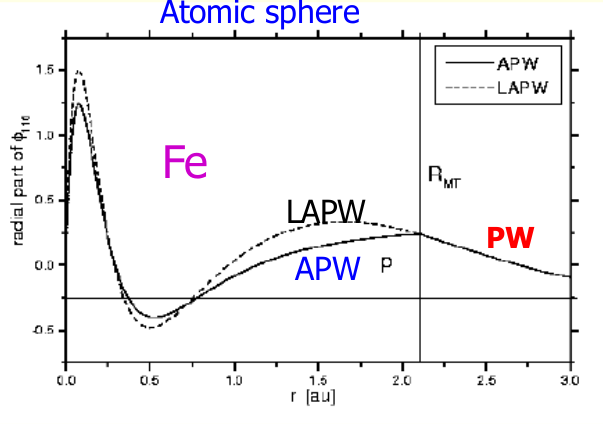
\includegraphics[height=1.20in,width=1.98in,viewport=1 20 585 435,clip]{WIEN2k-LAPW.png}
\caption{\small \textrm{Partitioning of the unit cell into atomic spheres(I) and an interstitial region(II)}}%(与文献\cite{EPJB33-47_2003}图1对比)
\label{Muffin_tin}
\end{figure}

为了提高LAPW方法的线性化程度(即提高基组的变分自由度),在同一能量范围处理半芯态(接近价态的能量较高的芯态)和价态,可采用外加基函数(与$\vec k$无关)方案,这部分外加基函数称为局域轨道(local orbitals, LO)\cite{PRB43-6388_1991,Singh}。由此构造的基函数包含两个指定能量的径向波函数和其中一个能量导数,这样的基函数即LAPW-LO:
\begin{equation}
  \phi_{lm}^{LO}(\vec r)=[A_{lm}u_l(E_{1,l},r)+B_{lm}\dot u_l(E_{1,l},r)+C_{lm}u_l(E_{2,l},r)]Y_{lm}(\hat{\vec r})
  \label{eq:LAPW-LO}
\end{equation}
根据条件$\phi_{lm}^{LO}$在MT球面上数值为零且保持一阶导数连续,并要求$\phi_{lm}^{LO}$在MT球内归一化,可以确定系数$A_{lm}$,$B_{lm}$,$C_{lm}$。

Sj\"ostedt等\cite{SSC114-15_2000}的计算表明,在标准LAPW方法中,将平面波展开使之在MT球面上与球内函数数值和一阶导数连续,这并非是实现Slater型APW方法最有效的线性化方法。采用指定能量参数$E_l$的APW形式的径向波函数[式\eqref{eq:APW-basis}],外加APW型局域轨道(local orbit, lo)扩展基函数,是更有效的方案,称为APW+lo。
\begin{equation}
  \varphi_{\vec k_i,\vec r}=\sum_{lm}[A_{lm}(\vec k_i)u_l(E_l,r)]Y_{lm}(\hat{\vec r})
  \label{eq:APW-basis}
\end{equation}
\begin{equation}
  \phi_{lm}^{lo}=[A_{lm}u_l(E_{1,l})+B_{lm}\dot u_l(E_{1,l})]Y_{lm}(\hat{\vec r})
  \label{eq:APW-lo}
\end{equation}
APW+lo基函数式\eqref{eq:APW-lo}形式上与标准LAPW式\eqref{eq:LAPW-basis}形式非常相似,但这里系数$A_{lm}$和$B_{lm}$与$\vec k$无关,是根据式\eqref{eq:APW-lo}在MT球边界上数值为零并且在MT球内归一化确定。这样构造的APW+lo基函数,总的波函数在MT球面上平滑且一阶可导的,但是根据式\eqref{eq:solid-115},在MT球面上有动能部分对Hamiltonian的贡献。为收敛到相同的结果,采用APW+lo基组比起标准LAPW基组小得多\cite{PRB64-195134_2001}。因此选择APW+lo基组比标准LAPW基组的计算效率要高。

WIEN2K程序包建议\cite{CPC59-399_1990,WIEN2K-UG_2001,CPC147-71_2002}一般平面波基函数收敛缓慢的轨道(比如过渡金属的3d态波函数)或MT球半径特别小的体系用APW+lo基组展开,其余价电子轨道用LAPW基组展开,此外对必要的半芯层可以用LO基组展开。用这样的方式可以同时考虑价态和半芯态。

\section{Green函数方法和muffin-tin轨道(muttin-tin orbitals, MTO)}
Green函数方法与APW方法非常相似,由Korringa\cite{P13-392_1947}与Kohn和Rostoker\cite{PR94-1111_1954}独立提出,又常称为KKR方法。KKR方法与前面介绍的OPW方法和APW方法最大的不同,它并非将晶体波函数按照某种选定的基函数展开求解久期方程,而是将Schr\"odinger方程变换成齐次积分方程的形式\cite{Ziman,Lizhengzhong}:
\begin{equation}
  \Psi_{\vec k}(\vec r)=\int_{\Omega_0}\tilde G_{\vec k}(\vec r-\vec r';E)V(\vec r')\Psi_{\vec k}(\vec r')d\vec r'
  \label{eq:solid-116}
\end{equation}
积分区间是整个WS原胞;$\tilde G_{\vec k}$是满足周期性边界条件的自由电子的Green函数,可以写成对晶体倒空间格矢的求和;
\begin{equation}
  \begin{split}
	  \tilde G_{\vec k}(\vec r-\vec r',E)&=-\frac1{4\pi}\sum_n\exp(\mathrm{i}\vec k\cdot\vec R_n)\frac{\cos q_0|\vec r-\vec r'-\vec R_n|}{|\vec r-\vec r'-\vec R_n|}\\
	  &=-\Omega_0^{-1}\sum_n\frac{\exp[\mathrm{i}(\vec k\cdot\vec G_n)(\vec r-\vec r')]}{|\vec k+\tilde G_n|-E}
  \end{split}
  \label{eq:solid-117}
\end{equation}
$q_0=\sqrt E$;$\tilde G_n$是倒格矢;$\vec R_n$是晶格平移格矢。Green函数
满足:
\begin{equation}
  (\nabla^2+E)\tilde G_{\vec k}(\vec r-\vec r';E)=\delta(\vec r-\vec r')
  \label{eq:solid-118}
\end{equation}

取间隙区MT势能为0,则积分式\eqref{eq:solid-116}中只有MT球内有非零球形对称势$V(r)$。$\tilde G_{\vec k}$可用球谐函数$Y_{lm}(\hat{\vec r})$,Bessel函数$j_l(x)$和Neumann函数$n_l(x)$展开,表示为方程\eqref{eq:solid-118}的特解$\tilde G_0$(在$\vec r=\vec r'$有奇点)和齐次方程通解$B_{\vec k}$两项之和:
\begin{equation}
  \begin{split}
    \tilde G_{\vec k}(\vec r-\vec r';E)=&\tilde G_0(\vec r-\vec r';E)+B_{\vec k}(\vec r-\vec r';E),\\
    \tilde G_0(\vec r-\vec r';E)=&-\frac1{4\pi}\frac{\cos(q_0|\vec r-\vec r'|)}{|\vec r-\vec r'|}=q_0\sum_{lm}j_l(q_0r)n_l(q_0r)\\
    &\times Y_{lm}(\hat{\vec r})Y_{lm}^{\ast}(\hat{\vec r'}),\quad r<r',\\
    B(\vec r-\vec r';E)=&\sum_{lm,l'm'}A_{lm,l'm'}j_l(q_0r)j_{l'}(q_0r')Y_{lm}(\hat{\vec r})Y_{l'm'}^{\ast}(\hat{\vec r}')
  \end{split}
  \label{eq:solid-119}
\end{equation}
选取KKR结构常数$A_{lm,l'm'}$使得$\tilde G_{\vec k}$满足Bloch定理。$A_{lm,l'm'}$可以表示为\cite{MCP8-251_1968}:
\begin{equation}
  A_{lm,l'm'}(\vec r,E)=4\pi q_0\sum_{\vec R_n\neq0}e^{i\vec k\cdot\vec R_n}\sum_{l''m''}i^{l'-l-l''}n_{l''}(q_0R_n)Y_{l''m''}^{\ast}(\hat{\vec R}_n)C_{lm,l'm',l''m''}
  \label{eq:solid-120}
\end{equation}
这里$C_{lm,l'm',l''m''}$是Gaunt系数,
%\begin{equation}
%  C_{lm,l'm',l''m''}=\int Y_{lm}(\vec r)Y_{l'm'}^{\ast}(\vec r)Y_{l''m''}(\vec r)d\Omega
%  \label{eq:solid-121}
%\end{equation}
结构常数是能量的函数,但只与给定$\vec k$点的晶体结构有关,而与晶体的势能无关。

KKR方程可用MT势的散射相移$\eta_l$来表示。在MT球面上,径向波函数可以表示为:
\begin{equation}
  u_l(E,R_{MT})=F_l[\cot\eta_l(q_0)j_l(q_0R_{MT})-\eta_l(q_0R_{MT})]
  \label{eq:solid-125}
\end{equation}
%代入式\eqref{eq:solid-124}并考虑到
%\begin{equation}
%  [n_l(q_0R_{MT}),j_l(q_0R_{MT})]=1/q_0R_{MT}^2
%  \label{eq:solid-126}
%\end{equation}

引入变分函数$\Lambda$:
\begin{equation}
  \Lambda=\int d\vec r\Psi_{\vec k}^{\ast}(\vec r)V(\vec r)\left[\Psi_{\vec k}(\vec r)-\int d\vec r'G_{\vec k}(\vec r-\vec r';E)V(\vec r')\Psi_{\vec k}(\vec r')\right]
  \label{eq:solid-122}
\end{equation}
给定能量$E$的尝试波函数和积分方程\eqref{eq:solid-116}用基函数展开,则求解变分方程$\delta\Lambda=0$\cite{PR94-1111_1954},
%Green函数方法中,
\begin{equation}
  \Psi_{\vec k}(E,\vec r)=\sum_{lm}C_{lm}u_l(r,E)Y_{lm}(\hat{\vec r}),\quad r\leqslant R_{MT}
  \label{eq:solid-123}
\end{equation}

%与APW方法相似,这里$u_l(r,E)$满足\eqref{eq:solid-110}的Schr\"odinger方程的径向解。将尝试波函数\eqref{eq:solid-123}代入式\eqref{eq:solid-122},通过变分得到一组线性方程,并确定系数$C_{lm}$\cite{MCP8-251_1968}
%\begin{equation}
%  \sum_{l'm'}\Lambda_{lm,l'm'}C_{l'm'}=0
%  \label{eq:solid-124}
%\end{equation}
%这里
%\begin{displaymath}
%  \begin{split}
%    \Lambda_{lm,l'm'}=j_l(q_0R_{MT})\{A_{lm,l'm'}[u_{l'}(E,R_{MT})&,j_{l'}(q_0R_{MT})]+q_0\delta_{lm,l'm'}[u_l,n_l]\},\\
%    [v_1,v_2]=v_1v_2'-v_2v_1'&,\quad v'(r)\equiv\frac{\partial v(r)}{\partial r}
%  \end{split}
%\end{displaymath}
可得KKR方法的久期方程
\begin{equation}
  \sum_{l'm'}(A_{lm,l'm'}+\sqrt E\cot\eta_l\delta_{lm,l'm'})F_{l'}C_{l'm'}=0
  \label{eq:solid-127}
\end{equation}
能量$E(\vec k)$只能取使久期行列式\eqref{eq:solid-128}为零的值:
\begin{equation}
  \det|A_{lm,l'm'}+\sqrt E\delta_{lm,l'm'}\cot\eta_l|=0
  \label{eq:solid-128}
\end{equation}
用这种方式,依赖于$l$的相移$\eta$可以表示为:
\begin{equation}
  \cot\eta_l=\dfrac{q_0n_l'(q_0R_{MT})-D_l(E,R_{MT})n_l(q_0R_{MT})}{q_0j_l'(q_0R_{MT})-D_l(E,R_{MT})j_l(q_0R_{MT})}
  \label{eq:solid-129}
\end{equation}
这里$D_l(E,R_{MT})=u_l'(E,R_{MT})/u_l(E,R_{MT})$。

KKR方法比APW方法更适用于计算具有近自由电子型的晶体能带结构,对过渡金属体系的计算,KKR方法对大的$l$值更容易收敛\cite{PPS86-337_1965,PR145-599_1966,Nemoshkalenko-Antonov},也更容易推广到无序体系。Jussouff和Zeller将KKR方法推广到WS原胞含有多个原子的复式晶格体系\cite{JPF11-1771_1981}。为了提高KKR方法的计算效率,人们提出了很多线性化近似的思想\cite{Andersen,PRB4-1064_1971,SSC11-799_1972,Andersen-unpub-1,Skriver}。其中最流行的是线性MT轨道(linear muffin-tin orbitals, LMTO)\cite{SSC13-133_1973,Andersen-unpub-2}。此外还有线性化KKR方法\cite{Ziesche-Lehmann,PSSB97-449_1980},线性化缀加Slater轨道(linear Augmented Slater orbitals, LASO)方法\cite{PRB29-2896_1984}。

%(1)原子球近似(Atomic sphere approximation, ASA)

与APW方法类似,根据WS原胞方法\cite{PR43-804_1933},%结构常数$A_{lm,l'm'}^{\vec k}(E)$
满足任意能量$E$的Schr\"odinger方程可以用分波(partial waves)表示:
\begin{equation}
  \Phi_{lm}(E,\vec r)\equiv u_l(E,r)i^lY_{lm}(\hat{\vec r})
  \label{eq:solid-130}
\end{equation}
这里$u_l$是径向Schr\"odinger方程的解。
%晶体中的价电子波函数可以表示为:
%\begin{equation}
%  \Psi_{\vec k}(\vec r,E)=\sum_{lm}C_{lm}(\vec k)\sum_{\vec R}e^{i\vec k\cdot\vec R}\theta(\vec r-\vec R)\Phi_{lm}(E,\vec r-\vec R)
%  \label{eq:solid-131}
%\end{equation}
%这里$\vec R$是晶格格矢,$\theta(\vec r)$是阶梯函数,在WS原胞内是1,原胞外为0。如果给定能量$E$和波矢$\vec k$,可以解出系数$C_{lm}$,使得$\Psi_{\vec}(\vec r,E)$及其导数是连续函数通过WS原胞边界与其他原胞连续。式\eqref{eq:solid-132}是晶体的Schr\"odinger方程的解。此时$E$是给定波矢$\vec k$的能量本征值。显然,边界条件依赖于$\vec k$和晶体结构。采用原子球近似(atomic sphere approximation, ASA),WS原胞由一个等体积的球代替,因为径向函数的对数导数可以表示为:
%\begin{equation}
%  D_l(E)=su_l'(E,s)/u_l(E,s)
%  \label{eq:solid-132}
%\end{equation}
%边界条件可以简化。这里球半径由条件$s=(3\Omega_0/4\pi)^{1/3}$得到;$\Omega_0$为WS原胞体积。

%由于对一般$\vec k$点,WS边界条件很难满足,如果采用各向同性的球形近似,这样的$\vec k$空间过于粗略。为了克服WS原胞方法的困难,Slater提出了MT球的假设\cite{PR51-846_1937}。根据MT近似,间隙区的势能为常数$V_c$,间隙区电子动能为:
%$$q_0^2=E-V)c$$
%用MT球之间的电子波的多极散射(multiple scattering)可以计算能带结构。

求解用相移表示的KKR方程
%\begin{equation}
%  \det|A_{lm,l'm'}^{\vec k}(E)+\delta_{lm,l'm'}q_0\cot\eta_l|=0
%  \label{eq:solid-133}
%\end{equation}
主要的困难在于,结构常数$A_{lm,l'm'}^{\vec k}$依赖于能量$E$。KKR方法中的势能
\begin{equation}
  q_0\cot\eta_l=q_0\dfrac{n_l(q_0s)D_l(E,s)-q_0sn_l'(q_0s)/n_l(q_0s)}{j_l(q_0s)D_l(E,s)-q_0sj_l'(q_0s)/j_l(q_0s)}
  \label{eq:solid-134}
\end{equation}
也%明显的
依赖于$q_0$。不过结构常数和势能对$q_0$的依赖很大程度上相互抵消\cite{PRB5-3894_1972,SSC11-395_1972,PRL27-1211_1971}。因此Andersen建议在原子球近似下应用KKR方法\cite{SSC13-133_1973}。
原子球近似下,间隙区体积为零,因此只须指定$q_0^2$($q_0^s$近似为原子球外的电子动能,Andersen采用$q_0^2=0$),这极大的简化了KKR方程,
\begin{equation}
  \det|S_{l'm',lm}^{\vec k}-\delta_{l'm',lm}P_l(E)|=0
  \label{eq:solid-135}
\end{equation}
这里势能为
\begin{equation}
  P_l(E)=2(2l+1)\frac{D_l(E)+l+1}{D_l(E)-l}
  \label{eq:solid-136}
\end{equation}
结构常数为
\begin{equation}
  S_{l'm',lm}^{\vec k}=\sum_{\vec R\neq0}e^{i\vec k\cdot\vec R}S_{l'm',lm}(\vec R)
  \label{eq:solid-137}
\end{equation}
这里
\begin{equation}
  \begin{split}
    S_{L',L}(\vec R)=&-\frac{8\pi(2l+2l'-1)!!}{(2l-1)!!(2l'-1)!!}\\
    &\times\sum_{L''}^{L''=L+L'}C_{L,L'',L'}(-i)^{l''}\left(\frac{R_s}s\right)^{-l''-1}Y_{L''}(\vec R)
  \end{split}
  \label{eq:solid-138}
\end{equation}
这里$L\hat=l,m$,$C_{L,L'',L'}$是Gaunt系数。%\eqref{eq:solid-121}。

因为结构常数\eqref{eq:solid-137}不再依赖于能量。关于晶体势能的信息只是势能的函数,而关于晶体结构的数据都包含在结构常数中。这种势能和晶体结构的分离很大程度上简化并加速了能带结构的计算。如果忽略间隙区动能的贡献,本征值的误差不会超过价带宽度的百分之几。当$q_0$$\rightarrow$0,%由方程\eqref{eq:solid-133}可以得到方程\eqref{eq:solid-135}
这就是KKR-ASA近似。采用ASA近似,对数导数$D_l(E)$包含原子大小和晶体势的信息,结构常数$S_{l'm',lm}(\vec k)$与能量无关,也与晶格常数无关。

%(2)MT轨道(MT orbitals)
假设MT球的球内势是球对称性的,球外间隙区电子动能$q_0^2=E-V_c=0$。考虑变量分离,MT球内电子波函数满足Schr\"odinger方程;间隙区满足Laplace方程$\nabla^2\Psi=0$。一般地说,径向波函数解的形式为$\Phi_l=a_lr^l+b_lr^{-l-1}$。系数$a_l$和$b_l$由波函数在MT球面上连续并且可导条件确定。因此径向波函数为:
\begin{displaymath}
  \Phi_l(r,E)=\left\{
  \begin{aligned}
    &u_l(r,E),&r\leqslant s\\
    &\left[\frac{D_l+l+1}{2l+1}\left(\frac rs\right)^l+\frac{l-D_l}{2l+1}\left(\frac rs\right)^{-l-1}\right]u_l(s,E),\quad&r>s
  \end{aligned}\right.
\end{displaymath}
这里$u_l(r,E)$是半径为$s$的MT球内归一化的径向Schr\"odinger方程的解。

该函数不能直接用作基函数,因为$r>s$部分的解包含发散的波函数,%因此,写出新的函数
%\begin{equation}
%   \Psi_l(r,D)=\left\{
%  \begin{aligned}
%    &\Phi_l(r,D)-\frac{D+l+1}{2l+1}\frac{\Phi_l(s,D)}{\Phi_l(s,l)}\Phi_l(r,l),\quad&r\leqslant s\\
%    &\frac{l-D}{2l+1}\left(\frac rs\right)^{-l-1}\Phi_l(s,D),&r>s
%  \end{aligned}\right.
 % \label{eq:solid-139}
%\end{equation}
%该表达式可以由$\Psi_l(r,E)$减去发散波$(D+l+1)(r/s)^l/(2l+1)$。而且对$r\leqslant s$将函数$(r/s)^l$代换为$\Psi_l(r,l)/\Psi_l(s,l)$,变量$E$替换为能量$E$对应的导数对数$D$。这种方法也可以用于波函数的节点已知的情形。函数\eqref{eq:solid-139}中MT球内部分不再是Schr\"odinger方程的解,但在整个空间是平滑的并且在球外衰减。将基函数写成:
%\begin{equation}
%  \Psi_{lm}(\vec r,D)=i^lY_{lm}(\hat{\vec r})\bar\Psi_l(r,D)
%  \label{eq:solid-140}
%\end{equation}
采用ASA近似,为推导基函数,必须包含由相对中心原子球距离$\vec R$处原子球的“函数尾巴”对中心原子球内函数的贡献。%写出Bloch求和
%\begin{equation}
%  \chi_{lm}^{\vec k}(\vec r,D)=\sum_{\vec R\neq0}e^{i\vec k\cdot\vec R}\bar\Phi_{lm}(\vec r-\vec R,D)
%  \label{eq:solid-141}
%\end{equation}
位于格点$\vec R$的“函数尾巴”%是$$\bar\Phi_{lm}(\vec r-\vec R,D)=i^lY_{lm}(\hat{\vec r}-\hat{\vec R})\left|\frac{\vec r-\vec R}s\right|^{-l-1}\frac{l-D}{2l+1}\Phi_l(s,D)$$将该函数
用求和定理(theorem of additivity)分解为相对于中心原子的角动量。
%\begin{equation}
%  \begin{split}
%    i^lY_{lm}(\hat{\vec r}-\hat{\vec R})\left|\frac{\vec r-\vec R}s\right|^{-l-1}=&4\pi\sum_{l''m'',l'm'}^{l''=l+l'}C_{lm,l''m'',l'm'}\frac{(2l''-1)!!}{(2l-1)!!(2l'+1)!!}\\
%    &\times(-i)^{l''}\left(\frac Rs\right)^{-l''-1}Y_{l''m''}^{\ast}(\hat{\vec R})\times i^{l'}\left(\frac rs\right)^{l'}Y_{l'm'}(\hat{\vec r})
%  \end{split}
%  \label{eq:solid-142}
%\end{equation}
%为了
保证函数在MT球面上连续可导,用$\Phi_{l'}(r,l')/\Phi_{l'}(s,l')$%\eqref{eq:solid-142}
替换$(r/s)^{l'}$,最后得到基函数\cite{Nemoshkalenko-Antonov}:
\begin{equation}
  \chi_{lm}^{\vec k}(\vec r,D)=\left\{
  \begin{aligned}
    \Phi_{lm}&(\vec r,D)-\Phi_l(s,D)(l-D)/(2l+1)&\\
    &\times\sum_{l'm'}\left[S_{l'm',lm}^{\vec k}-(l+1+D)/(l-D)2(2l+1)\delta_{l'm',lm}\right]\quad&\\
    &\times\Phi_{l'm'}(\vec r,l')/(\Phi_{l'}(s,l')2(2l'+1)), &r\leqslant s\\
    \Phi_l&(s,D)(l-D)/(2l+1)\left[i^lY_{lm}(\hat{\vec r})(r/s)^{-l-1}\right.+\sum_{l'm'}S_{l'm',lm}^{\vec k}&\\
    &\left.\times i^{l'}Y_{l'm'}(\hat{\vec r})(r/s)^{l'}/(2(2l'+1))\right],&r>s
  \end{aligned}\right.
  \label{eq:solid-143}
\end{equation}
这里$S_{l'm',lm}^{\vec k}$由式\eqref{eq:solid-137}确定。这就是MT轨道,可以用作变分的基函数。

注意到MT轨道的线性组合$$\Psi_{\vec k}(\vec r)=\sum_{lm}C_{lm}(\vec k)\sum_{\vec R}e^{i\vec k\cdot\vec R}\chi_{lm}(\vec k,\vec r-\vec R,D_l(E))$$是整个晶体的Schr\"odinger方程的解。%该式与式\eqref{eq:solid-131}等价
在中心原子球内(其他原子球一样),来自其他原子的“函数尾部”彼此抵消,中心原子MT球内的非球形部分正比于$i^lY_{lm}(\hat{\vec k})r^l$,也就是说式\eqref{eq:solid-143}中,$r\leqslant s$部分的第二项趋于零,得到方程%此条件给出一套线性齐次方程。
\begin{equation}
  \sum_{lm}[S_{l'm',lm}^{\vec k}-\delta_{l'm',lm}P_l(E)]\Phi_l(s,D_l)C_{lm}(\vec k)=0
  \label{eq:solid-144}
\end{equation}
如果采用由式\eqref{eq:solid-136}和式\eqref{eq:solid-137}定义的势能函数和结构常数,就可以得到KKR-ASA方程。

%(3)系综带结构(Canonical band structure)
%如果KKR-ASA方程中轨道角动量$l$是固定值,当结构常数中$l\neq l'$近似为零,称为系综带的结构。在这种情况下,子矩阵$S_{l'm',lm}^{\vec k}$对每个$l$值对角化独立的得到$(2l+1)$个非杂化的系综子能带$S_{li}(\vec k)$对应的本征矢为$u_{lm,li}(\vec k)$。因为势能只是依赖于$l$而与$m$无关,酉变换同时将使得KKR-ASA式\eqref{eq:solid-144}对角化。于是非杂化$nl$能带$E_{nli}(\vec k)$是方程
%\begin{equation}
%  S_{li}(\vec k)=2(2l+1)[D_l(E)+l+1]/[D_l(E)-l],\quad i=1,2,\cdots,2l+1
%  \label{eq:solid-145}
%\end{equation}
%的解。系综带只与晶体结构有关,其对原子类型与原子大小的依赖包含在势能函数$P_l(E)$中,通过关联电子态和给定原子的特征标量,势能函数将系综带变换为能带。杂化矩阵元的影响对带结构的影响很小,除非具有不同$l$值的系综带之间出现交叉。

%系综带的宽度可根据下式确定\cite{PhysicaB91-317_1977},
%\begin{displaymath}
%  \begin{split}
%    S_l^2&=(2l+1)^{-1}\sum_{i=1}^{2l+1}(2\pi)^{-3}\Omega_0\int d^3kS_{li}^2(k)\\
%    &=2^{l+2}(2l+1)\frac{(2l+1)(2l+3)\cdots(4l-1)}{l!}\sum_{R\neq0}\left(\frac sR\right)^{2(2l+1)}
%  \end{split}
%\end{displaymath}
%只与等同球的数目和它们的距离有关。系综带的带宽为$W_l\equiv(12S_l^2)^{1/2}$,对晶体结构为{\it fcc}\,{\it bcc}\,和{\it hcp}\,$(c/a=\sqrt{8/3})$的体系,$W_p$分别为18.8,18.7和18.6;而$W_d$分别为23.8,23.5和23.5。

%自洽KKR-ASA能带计算,每一步必须计算MT球内平均价电子密度
%\begin{equation}
%  \rho(r)=\frac1{4\pi}\sum_l\int^{\varepsilon_F}u_l^2(E,r)r^2N_l(E)dE
%  \label{eq:solid-146}
%\end{equation}
%这里分数态密度
%$$N_l(E)=2\sum_j(2\pi)^{-3}\Omega_0\int_{\Omega_0}d^3\vec k\sum_m|C_{lm;j}(\vec k)|^2\delta(E-E_j(\vec k))$$
%可以表示为\cite{Mackintosh}
%$$N_l(E)=\frac12\dot P_l(E)[\partial n(\mathbf P)/\partial P_l]|_{\mathbf P(E)}$$
%这里$P_l(E)$是势能函数\eqref{eq:solid-136},“矢量”定义为$\mathbf P\equiv\{P_s,P_p,P_d,\cdots\}$;$n(\mathbf P)$是包含全部结构数据的系综态数目。

%(4)线性MT轨道(linaer muffin-tin orbtials, LMTO)方法
用MT轨道作为基函数\eqref{eq:solid-143}表示的尝试波函数得到的MT轨道线性组合为:
\begin{equation}
  \det|\langle\chi_{l'm'}^{\vec k}(\vec r-\vec R_l')|\hat H-E|\chi_{lm}^{\vec k}(\vec r-\vec R_l)\rangle|=0
  \label{eq:solid-147}
\end{equation}
MTO方法与KKR方法复杂程度相当,但是MTO方法可以更好的考虑非MT晶体势且比KKR方法收敛更快。不过MTO隐含的依赖于能量,使得其计算量与APW和KKR方法相当。采用与LAPW类似的思想,选择能量参数与MTO无关,可以很好的简化问题\cite{PRB12-3060_1975}。

将基函数的径向波函数用Taylor级数在能量点$E_{\nu}$附近展开到一阶,
\begin{equation}
  \Phi(D,r)=\Phi_{\nu}(r)+\omega(D)\dot\Phi_{\nu}(r)
  \label{eq:solid-148}
\end{equation}
这里
$$\Phi_{\nu}(r)\equiv u_l(E_{\nu},r);\quad\dot\Phi_{\nu}\equiv\left.\frac{\partial u_l(E,r)}{\partial E}\right|_{E=E_{\nu}}$$
径向函数$\Phi_{\nu}(r)$在半径为$s$的原子球内是归一化的。系数$\omega(D)$,类似于$\Phi(D,r)$依赖于径向函数的对数导数,选择$\omega(D)$使得$\Phi(D,r)$在球面处有对数导数
\begin{equation}
  \omega(D)=-\frac{\Phi_{\nu}}{\dot\Phi_{\nu}}\frac{D-D_{\nu}}{D-D_{\dot\nu}}
  \label{eq:solid-149}
\end{equation}
这里
\begin{equation}
  D_{\nu}=S\Phi_{\nu}'(s)/\Phi_{\nu}(s)
  \label{equation-150}
\end{equation}
\begin{equation}
  D_{\dot\nu}=S\dot\Phi_{\nu}'(s)/\dot\Phi_{\nu}(s)
  \label{eq:solid-151}
\end{equation}
函数\eqref{eq:solid-148}在原子球面上的数值$\Phi(D,s)\equiv\Phi(D)$定义为
\begin{equation}
  \Phi(D)=\Phi_{\nu}\frac{D_{\nu}-D_{\dot\nu}}{D-D_{\dot\nu}}
  \label{eq:solid-152}
\end{equation}
%当基函数形式为
%\begin{equation}
%  \Phi_{lm}(D,\vec r)=i^lY_{lm}(\hat{\vec r})\Phi_l(D,r)
%  \label{eq:solid-153}
%\end{equation}
%球内的Hamiltonian矩阵元和重叠矩阵元可以表示为
%\begin{equation}
%  \langle\Phi_{l'm'}(D')|\vec H-E_{\nu}|\Phi_{lm}(D)\rangle=\delta_{l'm',lm}\omega_l(D),
%  \label{eq:solid-154}
%\end{equation}
%\begin{equation}
%  \langle\Phi_{l'm'}(D')|\Phi_{lm}(D)\rangle=\delta_{l'm',lm}(1+\langle\dot\Phi_{\nu l}^2\rangle\omega_l(D))
%  \label{eq:solid-155}
%\end{equation}
%定义$\Phi_{\nu}\equiv\Phi_{\nu}(s);\dot\Phi_{\nu}\equiv\dot\Phi_{\nu}(s)$。

晶体计算中,每个原子球对能谱的影响由势能参数$D_{\nu},s\Phi_{\nu}^2,s\Phi_{\nu}\dot\Phi_{\nu}$和$\langle\dot\Phi_{\nu}^2\rangle$组合得到,前三个参数依赖于所选择的能量$E_{\nu}$,因此实际应用中利用$D_1=-l-1$和$D_2=l$,将势能参数变化为$\omega(D_1),s\Phi^2(D_1)$和$\Phi(D_1)/\Phi(D_2)$更方便,于是式(\ref{eq:solid-148},\ref{eq:solid-149},\ref{eq:solid-151})分别具有如下形式:%使用参数$\omega(D_1),s\Phi^2(D_1)$和$\Phi(D_1)/\Phi(D_2)$,这里$D_1=-l-1,D_2=l$,将第一套参数换为第二套参数$D_1$和$D_2$实际上是用能量的正割函数而不再是正切函数。第二套参数使用更方便,式\eqref{eq:solid-148},\eqref{eq:solid-149},\eqref{eq:solid-151}具有如下形式:
\begin{equation}
  \begin{split}
   \Phi_l(r,D)=&\frac{\omega_l(D)-\omega_l(-l-1)}{\omega_l(l)-\omega_l(-l-1)}\Phi_l(l,r)\\
   &+\frac{\omega_l(D)-\omega_l(l)}{\omega_l(-l-1)-\omega_l(l)}\Phi_l(-l-1,r)
  \end{split}
  \label{eq:solid-156}
\end{equation}
\begin{equation}
  \frac{\omega_l(D)-\omega_l(-l-1)}{\omega_l(D)-\omega_l(l)}=\frac{\Phi_l(s,-l-1)}{\Phi_l(s,l)}\frac{D+l+1}{D-l}
  \label{eq:solid-157}
\end{equation}
\begin{equation}
  \Phi_l(s,D)=\frac{(2l+1)\Phi_l(s,-l-1)\Phi_l(s,l)}{(D+l+1)\Phi_l(s,-l-1)-(D-l)\Phi_l(s,l)}
  \label{eq:solid-158}
\end{equation}
同时可以得到下列关系
\begin{equation}
  \frac{\omega_l(D)-\omega_l(-l-1)}{\omega_l(l)-\omega_l(-l-1)}=\frac{D+l+1}{2l+1}\frac{\Phi_l(s,D)}{\Phi_l(s,l)}
  \label{eq:solid-159}
\end{equation}
\begin{equation}
  \frac{\omega_l(l)-\omega_l(D)}{\omega_l(l)-\omega_l(-l-1)}=\frac{l-D}{2l+1}\frac{\Phi_l(s,D)}{\Phi_l(s,-l-1)}
  \label{eq:solid-160}
\end{equation}
Andersen近似下,MT轨道\eqref{eq:solid-143}写成:
\begin{equation}
  \chi_{lm}^{\vec k}(\vec r,D)\simeq\frac{\omega_l(l)-\omega_l(D)}{\omega_l(l)-\omega_l(-l-1)}\chi_{lm}^{\vec k}(\vec r)=\alpha_l(D)\chi_{lm}^{\vec k}(\vec r)
  \label{eq:solid-161}
\end{equation}
这里MT轨道$\chi_{lm}^{\vec k}(\vec r)$与能量无关。
\begin{equation}
  \chi_{lm}^{\vec k}(\vec r)=\Phi_{lm}(\vec r,-l-1)-\Phi_l(s,-l-1)\sum_{l'm'}S_{l'm',lm}^{\vec k}\frac{\Phi_{l'm'}(\vec r,l')}{2(2l'+1)\Phi_{l'}(s,l')}
  \label{eq:solid-162}
\end{equation}
这里$S_{l'm',lm}^{\vec k}$是结构常数\eqref{eq:solid-137},可以表示为\cite{PRB12-3060_1975}:
\begin{equation}
  S_{l'm',lm}^{\vec k}=g_{l'm',lm}\Sigma_{\lambda\mu}^{\vec k}
  \label{eq:solid-163}
\end{equation}
这里$\lambda=l'+l$;$\mu=m'-m$;
\begin{displaymath}
  \begin{split}
    &g_{l'm',lm}=(-1)^{m+1}2\left(\frac{(2l'+1)(2l+1)}{2\lambda}\frac{(\lambda+\mu)!(\lambda-\mu)!}{(l'+m')!(l'-m')!(l+m)!(l-m)!}\right)^{1/2}\\
    &\Sigma_{\lambda\mu}^{\vec k}=\sum_{\vec R\neq0}e^{i\vec k\cdot\vec R}\left(\frac sR\right)^{\lambda+1}[\sqrt{4\pi}i^{\lambda}Y_{\lambda\mu}(\hat{\vec R})]^{\ast}
  \end{split}
\end{displaymath}
式\eqref{eq:solid-162}中的第二项来自于晶体中其余原子的“函数尾部”之和。因为用$\chi_{lm}^{\vec k}(\vec k,D)$替换为$\chi_{lm}^{\vec k}(\vec r)$写成$\alpha_l(D)$和能量无关的轨道的MTO表象使用方便。这种替换只是影响了波函数的归一化,而不会影响能量本征值。

式\eqref{eq:solid-162}的更一般的单中心展开的表达式为:
\begin{equation}
  \chi_{lm}^{\vec k}(D_{l2},\vec r)=\Phi_{lm}(D_{l2},\vec r)-\sum_{l'm'}\frac{\Phi_{l'm'}(l',\vec r)}{\omega_{l'}(D_{l_2'})-\omega_{l'}(l')}T_{l'm',lm}^{\vec k}
  \label{eq:solid-164}
\end{equation}
这里$D_{l_2}$是任意不等于$l$的对数导数;$T_{l'm',lm}^{\vec k}$是矩阵
\begin{equation}
  T_{l'm',lm}^{\vec k}(D_{l_2'},D_{l_2})=\sqrt{\frac s2}\Phi_{l'}(s,D_{l_2})\left\{-2(2l+1)\frac{D_{l_2}+l+1}{D_{l_2}-1}+S_{l'm',lm}^{\vec k}\right\}\sqrt{\frac s2}\Phi_l(s,D_{l_2})
  \label{eq:solid-165}
\end{equation}
实际应用中,一般采用$D_{l_2}=-l-1$,此时矩阵\eqref{eq:solid-165}可以简化为:
\begin{equation}
  T_{l'm',lm}^{\vec k}=\sqrt{\frac s2}\Phi_{l'}(s,-l'-1)S_{l'm',lm}^{\vec k}\sqrt{\frac s2}\Phi_l(s,-l-1)
  \label{eq:solid-166}
\end{equation}
Hamiltonian和重叠矩阵元表示为
\begin{equation}
  \begin{split}
    H_{l'm',lm}^{\vec k}=\langle\chi_{l'm'}^{\vec k}|\vec H|\chi_{lm}^{\vec k}=&H_{l'}^{(1)}\delta_{l'm',lm}+\left[-(H_{l'}^{(2)}+H_l^{(2)})S_{l'm',lm}^{\vec k}+\sum_{l''m''}S_{l'm',l''m''}^{\vec k}H_{l''}^{(3)}S_{l''m'',lm}^{\vec k}\right]\frac s2\\
    &\times\Phi_{l'}(s,-l'-1)\Phi_l(s,-l-1),
  \end{split}
  \label{eq:solid-167}
\end{equation}
\begin{equation}
  \begin{split}
    O_{l'm',lm}^{\vec k}=\langle\chi_{l'm'}^{\vec k}|\chi_{lm}^{\vec k}=&O_{l'}^{(1)}\delta_{l'm',lm}+\left[-(O_{l'}^{(2)}+O_l^{(2)})S_{l'm',lm}^{\vec k}+\sum_{l''m''}S_{l'm',l''m''}^{\vec k}O_{l''}^{(3)}S_{l''m'',lm}^{\vec k}\right]\frac s2\\
    &\times\Phi_{l'}(s,-l'-1)\Phi_l(s,-l-1),
  \end{split}
  \label{eq:solid-168}
\end{equation}
这里
\begin{equation}
  \begin{split}
    O_l^{(1)}&=1+\langle\dot\Phi_{\nu l}^2\rangle\omega_l^2(-l-1);\\
    O_l^{(2)}&=\frac{1+\langle\dot\Phi_{\nu l}^2\rangle\omega_l(-l-1)\omega_l(l)}{\omega_l(-l-1)-\omega_l(l)};\\
    O_l^{(3)}&=\frac{1+\langle\dot\Phi_{\nu l}^2\rangle\omega_l^2(-l)}{2s[(2l+1)\Phi_l(s,l)]^2};\\
    H_l^{(1)}&=\omega_l(-l-1)+E_{\nu l}O_l^{(1)};\\
    H_l^{(2)}&=\frac12+\frac{\omega_l(l)}{\omega_l(-l-1)-\omega_l(l)}+E_{\nu l}O_l^{(2)};\\
    H_l^{(3)}&=\frac{\omega_l(l)}{2s[(2l+1)\Phi_l(s,l)]^2}+E_{\nu l}O_l^{(3)};
  \end{split}
  \label{eq:solid-169}
\end{equation}
这里式\eqref{eq:solid-167}和\eqref{eq:solid-168}中形式为$S_{l'm',lm}^0$,$S_{l'm',lm}^1$和$S_{l'm',lm}^2$分别为单中心、双中心和三中心积分。式(\ref{eq:solid-167},\ref{eq:solid-168})是原子球近似的LMTO(LMTO-ASA)方法的基本表达式。该方法与LCAO方法很相似,不过LCAO方法主要困难在于处理多中心积分,而LMTO-ASA中,这些积分很容易处理。

放弃原子球近似而改用APW或者KKR方法中的MT球近似,可以得到LMTO方法。将WS原胞分为半径为s的彼此不相重叠的MT球区(区域I)和间隙区(区域II)两部分,MT球内具有球对称势,间隙区电子动能$q_0^2=E-V_c=0$,据此Hamiltonian和重叠矩阵为
\begin{equation}
  H_{l'm',lm}^{\vec k}=\langle\chi_{l'm'}^{\vec k}|\vec H|\chi_{lm}^{\vec k}\rangle-V_c\langle\tilde\chi_{l'm'}^{\vec k}|\tilde\chi_{lm}^{\vec k}\rangle+V_c\{\tilde\chi_{l'm'}^{\vec k}|\tilde\chi_{lm}^{\vec k}\},
  \label{eq:solid-170}
\end{equation}
\begin{equation}
  O_{l'm',lm}^{\vec k}=\langle\chi_{l'm'}^{\vec k}|\chi_{lm}^{\vec k}\rangle-\langle\tilde\chi_{l'm'}^{\vec k}|\tilde\chi_{lm}^{\vec k}\rangle+\{\tilde\chi_{l'm'}^{\vec k}|\tilde\chi_{lm}^{\vec k}\},
  \label{eq:solid-171}
\end{equation}
这里$\langle\cdots\rangle$表示对区域I积分,而$\{\cdots\}$是对整个$\Omega_0$的积分;$\chi_{lm}^{\vec k}$是定义在整个空间的自由电子的MT轨道。

MT轨道对两个区域的精确能量依赖关系由式\eqref{eq:solid-143}得到,根据Andersen近似,可以表示为\eqref{eq:solid-161}。能量无关的MT轨道函数形式为
\begin{equation}
  \chi_{lm}^{\vec k}(\vec r,-l-1)=\left\{
  \begin{aligned}
    \Phi_{lm}&(\vec r,-l-1)-\Phi_l(s,-l-1)&\\
    &\times\sum_{l'm'}S_{l'm',lm}^{\vec k}\Phi_{l'm'}(\vec r,l')/(2(2l'+1)\Phi_l(s,l')),&r\leqslant s,\\
    i^lY_{lm}&(\hat{\vec r})\Phi_l(s,-l-1)(r/s)^{-l-1}&\\
    &-\Phi_l(s,-l-1)\sum_{l'm'}S_{l'm',lm}^{\vec k}(i^{l'}Y_{l'm'}(\hat{\vec k})/(2(2l'+1)))(r/s)^{l'},\quad&r>s
  \end{aligned}\right.
  \label{eq:solid-172}
\end{equation}
%当整个空间满足$E=V_V_c$,对自由电子可以导出类似的函数,只是式\eqref{eq:solid-172}中$\Phi_l$和$\Phi_{lm}$,被对应的自由电子函数$\tilde\Phi_{lm}$和$\tilde\Phi_l$替代。在区间II,要保持函数$\tilde\chi_{lm}^{\vec k}(\vec r,-l-1)$与$\chi_{lm}^{\vec k}(\vec r,-l-1)$相等,必须在两个区域内$\tilde\chi_{lm}^{\vec k}$都乘上$\Phi_l(s,-l-1)/\tilde\Phi_l(s,-l-1)$,因此有基函数
%\begin{equation}
%  \tilde\chi_{lm}^{\vec k}(\vec r,-l-1)=\left\{
%  \begin{aligned}
%    \tilde\Phi_{lm}&(\vec r,-l-1)\Phi_l(s,-l-1)/\tilde\Phi_l(s,-l-1)-\Phi_l(s,-l-1)&\\
%    &\times\sum_{l'm'}S_{l'm',lm}^{\vec k}\tilde\Phi_{l'm'}(\vec r,l')/(2(2l'+1)\tilde\Phi_l(s,l')),&r\leqslant s,\\
%    i^lY_{lm}&(\hat{\vec r})\Phi_l(s,-l-1)(r/s)^{-l-1}-\Phi_l(s,-l-1)&\\
%    &\times\sum_{l'm'}S_{l'm',lm}^{\vec k}(i^{l'}Y_{l'm'}(\hat{\vec k})/(2(2l'+1)))(r/s)^{l'},\quad&r>s
%  \end{aligned}\right.
%  \label{eq:solid-173}
%\end{equation}

%LMTO-ASA方法使用近似\eqref{eq:solid-148},利用$D=-l-1$可以简化矩阵元,对自由电子的一个类似的近似是:
%\begin{equation}
%  \tilde\Phi_l(r,-l-1)=\tilde\Phi_{l\nu}(r)+\tilde\omega_l(-l-1)\dot{\tilde\Phi}_{l\nu}(r)
%  \label{eq:solid-174}
%\end{equation}
%用无穷小量$-\varepsilon$代替$(V-E)$,写出径向Schr\"odinger方程$(r/s)^l[1+(r/s)^2a_1+\cdots]$,简单变换,有
%\begin{equation}
%  \tilde\Phi_l(r,\varepsilon)=\sqrt{\frac{2l+3}{s^3}}\left[1+\frac{\varepsilon s^2}{2(2l+5)}\right]\left(\frac rs\right)^l\left[1-\frac{\varepsilon s^2}{2(2l+3)}\left(\frac rs\right)^2\right]
%  \label{eq:solid-175}
%\end{equation}
%由此有
%\begin{equation}
%  \tilde\Phi_{l\nu}=\sqrt{\frac{2l+3}{s^3}}\left(\frac rs\right)^l,
%  \label{eq:solid-176}
%\end{equation}
%\begin{equation}
%  \dot{\tilde\Phi}_{l\nu}=\sqrt{\frac{2l+3}{s^3}}\left[\left(\frac rs\right)^l\frac{s^2}{2(2l+5)}-\frac{s^2}{2(2l+3)}\left(\frac rs\right)^2\right]
%  \label{eq:solid-177}
%\end{equation}
%\begin{equation}
%  \tilde\Phi_l(s,-l-1)=\sqrt{\frac{2l+3}{s^3}}\frac{2l+5}{2(2l+5)}
%  \label{eq:solid-178}
%\end{equation}
在倒空间内表示,MT轨道的Bloch和为
\begin{equation}
  \tilde\chi_{lm}^{\vec k}(\vec r,-l-1)=\Phi_l(s,-l-1)\sum_{\vec G_n}e^{i\vec k_n\cdot\vec r}F_{lm}(\hat{\vec k}_n)
  \label{eq:solid-179}
\end{equation}
这里$\vec k_n=\vec k+\vec G_n$是倒格矢。
\begin{equation}
  F_{lm}(\vec k_n)=(2l+1)(2l+3)\frac{4\pi s^3}{\Omega_0}\frac{j_{l+1}(k_ns)}{(k_n s)^3}Y_{lm}(\hat{\vec k}_n)
  \label{eq:solid-180}
\end{equation}
对整个WS原胞积分
\begin{equation}
  \{\tilde\chi_{l'm'}^{\vec k}|\tilde\chi_{lm}^{\vec k}\}=\Omega_0\Phi_{l'}(R_{MT},-l'-1)\Phi_l(s,-l-1)\sum_{\vec G_n}F_{l'm'}^{\ast}(\vec k_n)F_{lm}(\vec k_n)
  \label{eq:solid-181}
\end{equation}
最后可得LMTO方法的矩阵元
\begin{equation}
  H_{l'm',lm}^{\vec k}=\bar H_{l'm',lm}^{\vec k}+V_c\{\tilde\chi_{l'm'}^{\vec k}|\tilde\chi_{lm}^{\vec k}\}
  \label{eq:solid-182}
\end{equation}
\begin{equation}
  O_{l'm',lm}^{\vec k}=\bar O_{l'm',lm}^{\vec k}+\{\tilde\chi_{l'm'}^{\vec k}|\tilde\chi_{lm}^{\vec k}\}
  \label{eq:solid-183}
\end{equation}
这里$\bar H_{l'm',lm}^{\vec k}$和$\bar O_{l'm',lm}^{\vec k}$由式\eqref{eq:solid-167}和\eqref{eq:solid-168}得到,式中的$H_{lm}^{(i)}$和$O_{lm}^{(i)}$用下列矩阵参数代替,
$$\bar H_{lm}^{(i)}=H_{lm}^{(i)}-V_cC_{lm}^{(i)},\quad\bar O_{lm}^{(i)}=O_{lm}^{(i)}-C_{lm}^{(i)},\quad i=1,2,3\cdots$$
这里
\begin{equation}
  \begin{split}
    &C_{lm}^{(1)}=\left[1+\frac{(2l+1)^2}{4(2l+3)(2l+7)}\right]\frac{4(2l+3)s^3\Phi_l^2(-l-1,s)}{(2l+5)^2};\\
    &C_{lm}^{(2)}=\frac{2s^2}{2(2l+1)(2l+5)};\\
    &C_{lm}^{(3)}=\frac{s^2}{2(2l+1)^2(2l+3)}.
  \end{split}
  \label{eq:solid-184}
\end{equation}
注意势能参数和结构参数都在MT球面上计算。类似的可以推导WS原胞内含有多个原子的体系\cite{Nemoshkalenko-Antonov}。

与LMTO方法平行的还有紧束缚(Tight-binding)LMTO方法\cite{Andersen-Jepsen,PRL53-2571_1984},全势(Full Potential)LMTO方法\cite{PRB37-10269_1988,Blochel,JCP87-7125_1987,PRB38-1537_1988,PRB46-12181_1992}。此外还有缀加球波(Augmented Spherical Wave, ASW)方法\cite{PRB19-6094_1979},线性KKR方法\cite{JPC5-97_1972,Wonn,Ziesche-Lehmann,PSSB97-449_1980},线性缀加Slater轨道(Linear Augmented Slater Orbitals, LASO)方法\cite{PRB29-2896_1984}等。
%Tight-Binding LMTO方法
%LMTO方法的一个不足之处在于MT轨道随半径衰减缓慢,距离中心MT球很远的WS原胞处的波函数贡献也不能忽略。注意到间隙区的MT轨道是Laplace方程$\nabla^2\Psi=0$的解,形式为:
%\begin{equation}
%  \begin{split}
%    K_{Rlm}(\vec r_R)&\equiv\left(\frac{r_R}s\right)^{-l-1}Y_{lm}(\hat{\vec r}_R)=-\sum_{l'm'}\left(\frac{r_{R'}}s\right)^{l'}\frac{Y_{l'm'}(\hat{\vec r}_{R'})}{2(2l'+1)}S_{R'l'm',Rlm}\\
%    &\equiv\sum_{l'm'}J_{R'l'm'}(\vec r_{R'})S_{R'l'm',Rlm}
%  \end{split}
%  \label{eq:solid-185}
%\end{equation}
%这里$J_{Rlm}$和$K_{Rlm}$分别是Laplace方程的正则化与非正则化解,$S_{R'l'm',Rlm}$是只与原子位置有关的系综结构矩阵,与势能参数或原子球半径无关。取矢量$\vec R-\vec R'$方向为坐标轴的$z$方向,系综结构常数有简单的形式\cite{Andersen-Jepsen},
%$$S_{ss\sigma}=-2(s/d),\quad S_{sp\sigma}=(2\sqrt3)(s/d)^2,\quad S_{pp(\sigma,\pi)}=6(s/d)^3(2,-1),$$
%$$S_{sd\sigma}=-2\sqrt5(s/d)^3,\quad S_{pd(\sigma,\pi)}=(6\sqrt5)(s/d)^4(-\sqrt3,3.1),$$
%或者$$S_{l'lm}=(-1)^{l+m+1}(l'+1)!2\left[\frac{(2l'+1)(2l+1)}{(l'+m)!(l'-m)!(l+m)!(l-m)!}\right]^{1/2}\left(\frac sd\right)^{l'+l+1}$$
%这里$s$是WS球半径,$d=|\vec R-\vec R'|$。由式\eqref{eq:solid-185}可知,{\it s}\,-轨道以$1/r$衰减;{\it p}\,-轨道以$1/r^2$衰减;{\it d}\,-轨道以$1/r^3$衰减,等等。这种波函数随半径缓慢衰减是数学上的,并非是金属中电子实际长程的反射行为。因此重新构造空间更局域的轨道将使得计算更方便,通过引入空间中快速衰减的“屏蔽”MT轨道,提出了紧束缚LMTO(tight-binding LMTO)方法\cite{Andersen-Jepsen,PRL53-2571_1984}。

%(1)屏蔽结构常数
%紧束缚LMTO方法的推导与其他的线性化方法相似,首先选择一套包络函数$\chi_G^i(\vec r)$,然后每个基函数在原子位置$\vec R$附近用球谐函数展开,每个分量及其导数上与$\Phi(r)$和$\dot\Phi(r)$的线性组合在球面$s_R$上连续。

%将MT轨道\eqref{eq:solid-143}写成Dirac记号,
%\begin{equation}
%  |K\rangle^{\infty}=|K\rangle-|J\rangle S
%  \label{eq:solid-186}
%\end{equation}
%这里$|K_{Rlm}\rangle^{\infty}$分布到整个空间,而$|K_{Rlm}\rangle$和$|J_{Rml}\rangle$在WS原胞外衰减,注意$|K\rangle$是矢量,其分量是函数$|K_{Rlm}(\vec r)\rangle$,$S$是矩阵,其矩阵元为$S_{R'l'm',Rlm}$。

%引入Laplace方程的新的正则解,
%\begin{equation}
%  |J^{\alpha}\rangle\equiv|J\rangle-|K\rangle\alpha
%  \label{eq:solid-187}
%\end{equation}
%这里$\alpha$是矩阵对角元。

%类似于式\eqref{eq:solid-186},屏蔽包络函数定义为
%\begin{equation}
%  |K^{\alpha}\rangle^{infty}\equiv|K\rangle-|J^{\alpha}\rangle S^{\alpha}
%  \label{eq:solid-188}
%\end{equation}
%将式\eqref{eq:solid-187}代入式\eqref{eq:solid-186},得到屏蔽结构矩阵方程,
%\begin{equation}
%  S^{\alpha}=S(I-\alpha S)^{-1}=[S^{-1}-\alpha]^{-1}=\alpha^{-1}[(\alpha^{-1}-S)^{-1}-\alpha]\alpha^{-1}
%  \label{eq:solid-189}
%\end{equation}
%或者等价的
%\begin{equation}
%  S^{\alpha}=S(I+\alpha S^{\alpha})=S+S\alpha S^{\alpha}
%  \label{eq:solid-190}
%\end{equation}
%局域化包络轨道(类比于静电的“屏蔽多极”)定义为
%\begin{equation}
%  |K^{\alpha}\rangle^{\infty}=|K\rangle^{\infty}(I-\alpha S)^{-1}=|K\rangle^{\infty}(I+\alpha S^{\alpha})
%  \label{eq:solid-191}
%\end{equation}
%或其解析形式
%\begin{equation}
%  K_{Rlm}^{\alpha}(\vec r_R)=\left(\frac{r_R}s\right)^{-l-1}Y_{lm}(\hat{\vec r}_R)+\sum_{R'}\sum_{l'=0}^{l_{\alpha}}\left(\frac{r_{R'}}s\right)^{-l'-1}\alpha_{R'l'}\sum_{m'}Y_{l'm'}(\hat{\vec r}_{R'})S_{R'l'm',Rlm}^{\alpha}
%  \label{eq:solid-192}
%\end{equation}
%由这些展开式可见$\alpha S^{\alpha}$可以看作“屏蔽电荷”。

%函数$K_{Rlm}^{\alpha}$也满足Laplace方程,因为它们是$K_{Rlm}$和$J_{Rlm}$的线性组合。但与$K_{Rlm}$不同,这些函数随半径快速收敛。

%选取$\alpha$使得$S^{\alpha}$和$K^{\alpha}\rangle^{\infty}$最短程,对于$l>2$,使用条件$\alpha_l=0$。

%局域MT轨道
Madelung\cite{PZ19-524_1918}最早研究了晶体中Coulomb势求和问题。1921年Ewald\cite{AP64-253_1921}发展了一般的晶体Coulomb势求和技术,此后Ewald方法得到了进一步的改进和推广\cite{Tosi,PR117-1466_1960,PR181-1020_1969}。

文献\cite{JMP22-2433_1981}提出了根据电荷密度多极展开和MT球面上的Dirichlet问题求解Poisson方程的全势(Full-Potential)方法:
%MT球半径$R_{MT}$外点$\vec r$处的Coulomb势为\cite{Landau-Lifshitz}
%\begin{equation}
%  V_I(\vec r)=\sum_L\frac{4\pi}{2l+1}q_l\frac{Y_L(\hat{\vec r})}{r^{l+1}}
%  \label{eq:solid-65}
%\end{equation}
%这里I表示间隙区;$Y_L(\hat{\vec r})$是球谐函数,$L\hat=l,m$;$q_l$是多极矩,
%\begin{equation}
%   q_l=\int_{\Omega_0}Y_L^{\ast}(\hat{\vec r})r^l\rho(\vec r)d^3r
%  \label{eq:solid-66}
%\end{equation}
将电子密度$\rho(\vec r)$分为MT球内部分$\rho_s(\vec r)$和间隙区部分$\rho_I(\vec r)$,$\rho(\vec r)=\rho_I(\vec r)\theta(r\in I)+\rho_s(\vec r)\theta(r\in \Omega_s)$
%\begin{equation}
%  \rho(\vec r)=\rho_I(\vec r)\theta(r\in I)+\rho_s(\vec r)\theta(r\in \Omega_s)
%  \label{eq:solid-67}
%\end{equation}
%在推导Coulomb势的时候,首先确定间隙区势能,再对MT球面解Dirichlet边条件得到球内的Coulomb势。
间隙区电子密度$\rho_I(\vec r)$是平缓函数,可以表示为快速收敛的Fourier级数。MT球内的的电子密度是强烈振荡的函数,其Fourier展开级数收敛缓慢。注意到间隙区Coulomb势对通过多极矩$q_L$依赖于MT球内电子密度\cite{Landau-Lifshitz}。因此可以用一个平缓的赝电子密度(Pseudo-density)函数替代MT球内的真实电子密度,使得两者具有相同的多极矩$q_L$。%:
%\begin{equation}
%  \rho(\vec r)\rightarrow\tilde\rho(\vec r)=\rho_I\theta(r\in I)+\tilde\rho_s(\vec r)\theta(r\in \Omega_s)
%  \label{eq:solid-68}
%\end{equation}
%要求赝电荷密度$\tilde\rho(\vec r)$可以用快速收敛的Fourier级数表示:
%\begin{equation}
%  \tilde\rho(\vec r)=\sum_{\vec G}[\rho_I(\vec G)+\tilde\rho_s(\vec G)]e^{i\vec G\cdot\vec r}
%  \label{eq:solid-69}
%\end{equation}
求解Poisson方程,通过赝电荷密度得到正确的间隙区Coulomb势,
\begin{equation}
  V_I(\vec r)=\sum_{\vec G}\frac{4\pi}{G^2}[\rho_I(\vec G)+\tilde\rho_s(\vec G)]e^{i\vec G\cdot\vec r}
  \label{eq:solid-70}
\end{equation}
%必须得到MT球内的赝电荷的Fourier展开$\tilde\rho_s(\vec G)$。

%将晶体中的电子密度表示为
%\begin{equation}
%   \rho(\vec r)=\rho_I(\vec r)+[\rho_s(\vec r)-\rho_I(\vec r)]\theta(r\in \Omega_s)
%  \label{eq:solid-71}
%\end{equation}
%这里第一项$\rho_I(\vec r)$定义在整个WS原胞内。MT球内的赝电荷密度可以表示成级数:
%\begin{equation}
%   \tilde\rho_s(\vec r)=\sum_LQ_LY_L(\hat{\vec r})\sum_{\nu}a_{\nu}r^{l+2\nu},\quad v=0,1,2,\cdots
%  \label{eq:solid-72}
%\end{equation}
%其中$a_{\nu}$是参数,$Q_L$是常数,它使得赝电荷与实际电荷的多极矩相匹配,即
%\begin{equation}
%  \tilde q_L=\sum_{L'}Q_{L'}\int_{\Omega_s}Y_L^{\ast}(\hat{\vec r})Y_{L'}(\hat{\vec r})d\Omega\int_0^{R_{MT}}\sum_{\nu}a_{\nu}r^{2(l+\nu+1)}dr
%  \label{eq:solid-73}
%\end{equation}
%或者
%\begin{equation}
%  Q_L=\tilde q_L\left[\sum_{\nu}\dfrac{R_{MT}^{2(l+\nu)+3}}{2(l+\nu)+3}\right]^{-1}
%  \label{eq:solid-74}
%\end{equation}
%这里$\tilde q_L$是电子密度\eqref{eq:solid-71}在MT球内的多极矩,$\tilde q_L=-Z\delta_{l0}+q_L-q_L^I$。$q_L$由式\eqref{eq:solid-66}计算得到,$q_L^I$是平面波电荷密度的多极矩
%\begin{equation}
%  \begin{split}
%   q_L^I=&\frac{\sqrt{4\pi}}3R_{MT}^3\rho_I(\vec G)\delta_{l0}\delta_{G0} \\
%   &+\sum_{\vec G\neq0}4\pi i^l\rho_I(\vec G)R_{MT}^{l+3}\dfrac{j_{l+1}(GR_{MT})}{GR_{MT}}Y_L^{\ast}(\vec G)
%  \end{split}
%  \label{eq:solid-75}
%\end{equation}
%其中$R_{MT}$是球半径。

MT球内赝电荷密度%\eqref{eq:solid-72}
的Fourier展开$\tilde\rho_s(\vec G)$%=\dfrac1{\Omega_0}\displaystyle\int_{\Omega_s}\tilde\rho_s(\vec r)e^{-i\vec G\cdot\vec r}d^3\vec r$
可以表示为\cite{JMP22-2433_1981}:
\begin{equation}
  \tilde\rho_s(\vec G)=\frac{4\pi}{\Omega_0}\sum_L\dfrac{(-i)^l(2l+2n+3)!!}{R_{MT}^l(2l+1)!!}\dfrac{j_{l+n+1}(GR_{MT})}{(GR_{MT})^{n+1}}\tilde q_Le^{-i\vec G\cdot\vec r}Y_L(\vec G)
  \label{eq:solid-76}
\end{equation}
其中$\Omega_0$是WS原胞体积。$n$是使得MT球内赝电荷平缓的参数。文献\cite{JMP22-2433_1981}给出了参数$n$的推荐值。

式\eqref{eq:solid-70}表明,MT球内赝电荷密度决定了间隙区Coulomb势能,
%但是不能用它来求解Poisson方程。
为了求得MT球内的Coulomb势,使用Dirichlet的球边界条件\cite{Landau-Lifshitz}和MT球面上的势能$V_I(\vec r_{MT})$,可以得到MT球内的Coulomb势:
\begin{displaymath}
%\begin{equation}
  V_s(\vec r)=\int_{\Omega_s}\rho_s(\vec r')G(\vec r,\vec r')d^3\vec r'-\dfrac{R_{MT}^2}{4\pi}\ointop\nolimits_sV_I(\vec r_{MT}')\frac{\partial G}{\partial n'}dS'
  \label{eq:solid-77}
%\end{equation}
\end{displaymath}
$\vec r_{MT}$表示MT球面上的点,G是格林函数。%:
%\begin{equation}
%  G(\vec r,\vec r')=4\pi\sum_L\dfrac{Y_L^{\ast}(\vec r')Y_L(\vec r)}{2l+1}\dfrac{r_<^l}{r_>^{l+1}}\left[1-\biggl(\dfrac{r_>}{R_{MT}}\biggr)^{2l+1}\right]
%  \label{eq:Green-function}
%\end{equation}
%其中$r_>$($r_<$)是$r$和$r'$中较大(较小)的一项。格林函数的导数:
%\begin{equation}
%  \frac{\partial G}{\partial n'}=\left.\frac{\partial G}{\partial r'}\right|_{r'=R_{MT}}=-\frac{4\pi}{R_{MT}^2}\sum_L\biggl(\dfrac r{R_{MT}}\biggr)^lY_L^{\ast}(\vec r')Y_L(\vec r)
%  \label{eq:derivative-Green}
%\end{equation}
%最后,
MT球内的Coulomb势可以表示为:
\begin{displaymath}
%\begin{equation}
  \begin{split}
    V_C(\vec r)=&\sum_LY_L(\vec r)\left[\frac{4\pi}{2l+1}\left\{\dfrac1{r^{l+1}}\int_0^rdr'(r')^{l+2}\rho_L(r')+r^l\int_r^{R_{MT}}dr'(r')^{1-l}\rho_L(r')\right\}\right.\\
    &+\biggl(\dfrac r{R_{MT}}\biggr)^l4\pi i^l\sum_{\vec G\neq0}\frac{4\pi}{G^2}\tilde\rho(\vec G)Y_L^{\ast}(\vec G)\left.\dfrac{GR_{MT}j_{l-1}(GR_{MT})}{2l+1}\right]
  \end{split}
%  \label{eq:solid-78}
%\end{equation}
\end{displaymath}
选定能带计算方法和波函数后,即可计算得到$\rho_L(\vec r)$和$\rho_I(\vec G)$的解析表达式。


\section{KKR方法、muffin-tin轨道(muttin-tin orbitals, MTO)和LMTO}
\subsection{KKR方法}
Green函数方法%与APW方法非常相似,
是由Korringa\cite{P13-392_1947}与Kohn和Rostoker\cite{PR94-1111_1954}独立提出,因此又被称为KKR方法。KKR方法的基本思想是多重散射理论(multiple scattering theory,如图\ref{Multi-scattering}所示),与前面介绍的OPW方法和APW方法最大的不同,KKR方法是将Schr\"odinger方程变换成齐次积分方程的形式,而不是将晶体波函数按照某种选定的基函数展开求解久期方程\cite{Ziman,Lizhengzhong}:
\begin{figure}[h!]
\centering
%\includegraphics[height=1.80in,width=1.95in,viewport=5 0 515 495,clip]{Figures/multiple-scattering_theory.png}
\includegraphics[height=1.70in,width=1.82in,viewport=5 0 515 495,clip]{multiple-scattering_theory.png}
\caption{\small \textrm{Central idea of multiple scattering theory:~ decomposition of electronic motion into scattering at atomic sites and free-electron like propagation in between. The bottom of the figure gives a sketch for the potential along the dashed line.}}
\label{Multi-scattering}
\end{figure}
\begin{equation}
  \Psi_{\vec k}(\vec r)=\int_{\Omega_0}\tilde G_{\vec k}(\vec r-\vec r^{\prime};E)V(\vec r^{\prime})\Psi_{\vec k}(\vec r^{\prime})d\vec r^{\prime}
  \label{eq:solid-116}
\end{equation}

积分区间是整个WS原胞;$\tilde G_{\vec k}$是满足周期性边界条件的自由电子的Green函数,它是Helmholtz方程
\begin{equation}
  (\nabla^2+E)\tilde G_{\vec k}(\vec r-\vec r^{\prime};E)=\delta(\vec r-\vec r^{\prime})
  \label{eq:solid-118}
\end{equation}
的解,可分别用晶体正空间格矢和倒空间格矢展开为
\begin{equation}
  \begin{split}
	  \tilde G_{\vec k}(\vec r-\vec r^{\prime},E)&=-\frac1{4\pi}\sum_n\exp(\mathrm{i}\vec k\cdot\vec R_n)\frac{\cos q_0|\vec r-\vec r^{\prime}-\vec R_n|}{|\vec r-\vec r^{\prime}-\vec R_n|}\\
	  &=-\Omega_0^{-1}\sum_n\frac{\exp[\mathrm{i}(\vec k\cdot\vec G_n)(\vec r-\vec r^{\prime})]}{|\vec k+\tilde G_n|-E}
  \end{split}
  \label{eq:solid-117}
\end{equation}
$q_0=\sqrt E$;$\tilde G_n$是倒格矢;$\vec R_n$是晶格平移格矢。

取间隙区MT势能为0,则积分式\eqref{eq:solid-116}中只有MT球内有非零球形对称势$V(r)$。在球坐标下,$\tilde G_{\vec k}$可用球谐函数$Y_{lm}(\hat{\vec r})$,Bessel函数$j_l(x)$和Neumann函数$n_l(x)$展开,表示为方程\eqref{eq:solid-118}的特解$\tilde G_0$(在$\vec r=\vec r^{\prime}$有奇点)和齐次方程通解$B_{\vec k}$两项之和:
\begin{equation}
  \begin{split}
    \tilde G_{\vec k}(\vec r-\vec r^{\prime};E)=&\tilde G_0(\vec r-\vec r^{\prime};E)+B_{\vec k}(\vec r-\vec r^{\prime};E),\\
    \tilde G_0(\vec r-\vec r^{\prime};E)=&-\frac1{4\pi}\frac{\cos(q_0|\vec r-\vec r^{\prime}|)}{|\vec r-\vec r^{\prime}|}=q_0\sum_{lm}j_l(q_0r)n_l(q_0r)\\
    &\times Y_{lm}(\hat{\vec r})Y_{lm}^{\ast}(\hat{\vec r}^{\prime}),\quad r<r^{\prime},\\
    B(\vec r-\vec r^{\prime};E)=&\sum_{lm,l^{\prime}m^{\prime}}A_{lm,l^{\prime}m^{\prime}}j_l(q_0r)j_{l^{\prime}}(q_0r^{\prime})Y_{lm}(\hat{\vec r})Y_{l^{\prime}m^{\prime}}^{\ast}(\hat{\vec r}^{\prime})
  \end{split}
  \label{eq:solid-119}
\end{equation}
合理选取KKR结构常数$A_{lm,l^{\prime}m^{\prime}}$使得$\tilde G_{\vec k}$满足Bloch定理。$A_{lm,l^{\prime}m^{\prime}}$可以表示为\cite{MCP8-251_1968}:
\begin{equation}
	A_{lm,l^{\prime}m^{\prime}}(\vec r,E)=4\pi q_0\sum_{\vec R_n\neq0}e^{\mathrm{i}\vec k\cdot\vec R_n}\sum_{l^{\prime\prime}m^{\prime\prime}}\mathrm{i}^{l^{\prime}-l-l^{\prime\prime}}n_{l^{\prime\prime}}(q_0R_n)Y_{l^{\prime\prime}m^{\prime\prime}}^{\ast}(\hat{\vec R}_n)C_{lm,l^{\prime}m^{\prime},l^{\prime\prime}m^{\prime\prime}}
  \label{eq:solid-120}
\end{equation}
这里$C_{lm,l^{\prime}m^{\prime},l^{\prime\prime}m^{\prime\prime}}$是Gaunt系数,
%\begin{equation}
%  C_{lm,l^{\prime}m^{\prime},l^{\prime\prime}m^{\prime\prime}}=\int Y_{lm}(\vec r)Y_{l^{\prime}m^{\prime}}^{\ast}(\vec r)Y_{l^{\prime\prime}m^{\prime\prime}}(\vec r)d\Omega
%  \label{eq:solid-121}
%\end{equation}
结构常数是能量的函数,但只与给定$\vec k$点的晶体结构有关,而与晶体的势能无关。

在MT近似下,根据散射理论,KKR方程的解可用散射相移$\eta_l$来表示,在MT球面上,径向波函数可以表示为:
\begin{equation}
  u_l(E,R_{MT})=F_l[\cot\eta_l(q_0)j_l(q_0R_{MT})-\eta_l(q_0R_{MT})]
  \label{eq:solid-125}
\end{equation}
%代入式\eqref{eq:solid-124}并考虑到
%\begin{equation}
%  [n_l(q_0R_{MT}),j_l(q_0R_{MT})]=1/q_0R_{MT}^2
%  \label{eq:solid-126}
%\end{equation}

为确定KKR方法的久期方式,引入变分函数$\Lambda$:
\begin{equation}
  \Lambda=\int d\vec r\Psi_{\vec k}^{\ast}(\vec r)V(\vec r)\left[\Psi_{\vec k}(\vec r)-\int d\vec r^{\prime}G_{\vec k}(\vec r-\vec r^{\prime};E)V(\vec r^{\prime})\Psi_{\vec k}(\vec r^{\prime})\right]
  \label{eq:solid-122}
\end{equation}
给定能量$E$的尝试波函数和积分方程\eqref{eq:solid-116}用基函数展开,\begin{equation}
  \Psi_{\vec k}(E,\vec r)=\sum_{lm}C_{lm}u_l(r,E)Y_{lm}(\hat{\vec r}),\quad r\leqslant R_{MT}
  \label{eq:solid-123}
\end{equation}

%与APW方法相似,这里$u_l(r,E)$满足\eqref{eq:solid-110}的Schr\"odinger方程的径向解。将尝试波函数\eqref{eq:solid-123}代入式\eqref{eq:solid-122},通过变分得到一组线性方程,并确定系数$C_{lm}$\cite{MCP8-251_1968}
%\begin{equation}
%  \sum_{l^{\prime}m^{\prime}}\Lambda_{lm,l^{\prime}m^{\prime}}C_{l^{\prime}m^{\prime}}=0
%  \label{eq:solid-124}
%\end{equation}
%这里
%\begin{displaymath}
%  \begin{split}
%    \Lambda_{lm,l^{\prime}m^{\prime}}=j_l(q_0R_{MT})\{A_{lm,l^{\prime}m^{\prime}}[u_{l^{\prime}}(E,R_{MT})&,j_{l^{\prime}}(q_0R_{MT})]+q_0\delta_{lm,l^{\prime}m^{\prime}}[u_l,n_l]\},\\
%    [v_1,v_2]=v_1v_2^{\prime}-v_2v_1^{\prime}&,\quad v^{\prime}(r)\equiv\frac{\partial v(r)}{\partial r}
%  \end{split}
%\end{displaymath}

则求解变分方程$\delta\Lambda=0$\cite{PR94-1111_1954},可得KKR方法的久期方程
\begin{equation}
  \sum_{l^{\prime}m^{\prime}}(A_{lm,l^{\prime}m^{\prime}}+\sqrt E\cot\eta_l\delta_{lm,l^{\prime}m^{\prime}})F_{l^{\prime}}C_{l^{\prime}m^{\prime}}=0
  \label{eq:solid-127}
\end{equation}
能量$E(\vec k)$只能取使久期行列式\eqref{eq:solid-128}为零的值:
\begin{equation}
  \det|A_{lm,l^{\prime}m^{\prime}}+\sqrt E\delta_{lm,l^{\prime}m^{\prime}}\cot\eta_l|=0
  \label{eq:solid-128}
\end{equation}
用这种方式,依赖于$l$的相移$\eta$可以表示为:
\begin{equation}
  \cot\eta_l=\dfrac{q_0n_l^{\prime}(q_0R_{MT})-D_l(E,R_{MT})n_l(q_0R_{MT})}{q_0j_l^{\prime}(q_0R_{MT})-D_l(E,R_{MT})j_l(q_0R_{MT})}
  \label{eq:solid-129}
\end{equation}
这里$D_l(E,R_{MT})=u_l^{\prime}(E,R_{MT})/u_l(E,R_{MT})$。

求解用相移表示的KKR方程
%\begin{equation}
%  \det|A_{lm,l^{\prime}m^{\prime}}^{\vec k}(E)+\delta_{lm,l^{\prime}m^{\prime}}q_0\cot\eta_l|=0
%  \label{eq:solid-133}
%\end{equation}
主要的困难在于,结构常数$A_{lm,l^{\prime}m^{\prime}}^{\vec k}$依赖于能量$E$。KKR方法中的势能
\begin{equation}
  q_0\cot\eta_l=q_0\dfrac{n_l(q_0s)D_l(E,s)-q_0sn_l^{\prime}(q_0s)/n_l(q_0s)}{j_l(q_0s)D_l(E,s)-q_0sj_l^{\prime}(q_0s)/j_l(q_0s)}
  \label{eq:solid-134}
\end{equation}
也%明显的
依赖于$q_0$。不过结构常数和势能对$q_0$的依赖很大程度上相互抵消\cite{PRB5-3894_1972,SSC11-395_1972,PRL27-1211_1971}。因此Andersen建议在原子球近似(atomic sphere approximation, ASA,如图\ref{Atomic_sphere-appro}所示)下应用KKR方法\cite{SSC13-133_1973}。
\begin{figure}[h!]
\centering
\includegraphics[height=1.20in,width=2.42in,viewport=5 0 1005 495,clip]{Atomic_sphere-appro.png}
\caption{\small \textrm{Atomic sphere approximation (ASA) in which the MT spheres are chosen to have the same volume as the Wigner-Seitz cell, which leads to overlapping spheres.}}
\label{Atomic_sphere-appro}
\end{figure}
在原子球近似下,间隙区体积为零,因此只须指定$q_0^2$($q_0^s$近似为原子球外的电子动能,Andersen取$q_0^2=0$),得到极大地简化的KKR-ASA方程,
\begin{equation}
  \det|S_{l^{\prime}m^{\prime},lm}^{\vec k}-\delta_{l^{\prime}m^{\prime},lm}P_l(E)|=0
  \label{eq:solid-135}
\end{equation}
其中势能函数为
\begin{equation}
  P_l(E)=2(2l+1)\frac{D_l(E)+l+1}{D_l(E)-l}
  \label{eq:solid-136}
\end{equation}
此时结构常数化简为
\begin{equation}
	S_{l^{\prime}m^{\prime},lm}^{\vec k}=\sum_{\vec R\neq0}e^{\mathrm{i}\vec k\cdot\vec R}S_{l^{\prime}m^{\prime},lm}(\vec R)
  \label{eq:solid-137}
\end{equation}
这里
\begin{equation}
  \begin{split}
    S_{L^{\prime},L}(\vec R)=&-\frac{8\pi(2l+2l^{\prime}-1)!!}{(2l-1)!!(2l^{\prime}-1)!!}\\
    &\times\sum_{L^{\prime\prime}}^{L^{\prime\prime}=L+L^{\prime}}C_{L,L^{\prime\prime},L^{\prime}}(-\mathrm{i})^{l^{\prime\prime}}\left(\frac{R_s}s\right)^{-l^{\prime\prime}-1}Y_{L^{\prime\prime}}(\vec R)
  \end{split}
  \label{eq:solid-138}
\end{equation}
这里$L\hat=l,m$,$C_{L,L^{\prime\prime},L^{\prime}}$是Gaunt系数。%\eqref{eq:solid-121}。

因为结构常数\eqref{eq:solid-137}不再依赖于能量。关于晶体势能的信息只是势能的函数,而关于晶体结构的数据都包含在结构常数中。这种势能和晶体结构的分离很大程度上简化并加速了能带结构的计算。如果忽略间隙区动能的贡献,本征值的误差不会超过价带宽度的百分之几。当$q_0$$\rightarrow$0,%由方程\eqref{eq:solid-133}可以得到方程\eqref{eq:solid-135}
这就是KKR-ASA近似。采用ASA近似,对数导数$D_l(E)$包含原子大小和晶体势的信息,结构常数$S_{l^{\prime}m^{\prime},lm}(\vec k)$与能量无关,也与晶格常数无关。

KKR方法比APW方法更适用于计算具有近自由电子型的晶体能带结构,对过渡金属体系的计算,KKR方法对大的$l$值更容易收敛\cite{PPS86-337_1965,PR145-599_1966,Nemoshkalenko-Antonov},也更容易推广到无序体系。Jussouff和Zeller将KKR方法推广到WS原胞含有多个原子的复式晶格体系\cite{JPF11-1771_1981}。在计算物理发展的早起,KKR方法因为简易高效,应用得比较多,但是随着计算方法和计算机技术的进步,对计算精度的要求越来越高,KKR方法已经很少使用了。
%为了提高KKR方法的计算效率,人们提出了很多线性化近似的思想\cite{Andersen,PRB4-1064_1971,SSC11-799_1972,Andersen-unpub-1,Skriver}。其中最流行的是线性MT轨道(linear muffin-tin orbitals, LMTO)\cite{SSC13-133_1973,Andersen-unpub-2}。此外还有线性化KKR方法\cite{Ziesche-Lehmann,PSSB97-449_1980},线性化缀加Slater轨道(linear Augmented Slater orbitals, LASO)方法\cite{PRB29-2896_1984}。

%(1)原子球近似(Atomic sphere approximation, ASA)

\subsection{MTO与LMTO}
KKR方法中,体系电子波函数的展开方式由散射理论确定,也就是波函数的分波(partial waves)表示。KKR方法的核心思想是构造Green函数,用积分方程代替Schr\"odinger方程的求解,因此要求Green函数满足Bloch定理的周期边界条件。实际上也可以选择分波作为基函数,用APW方法类似的思想构造基函数求解偏微分方程,这就是MTO方法\cite{Andersen,PRB4-1064_1971,SSC11-799_1972,Andersen-unpub-1,Skriver,Xu-Li-II},在数学表示形式上,MTO方法与KKR方法关系更密切。

根据电子散射和WS原胞的思想\cite{PR43-804_1933},%结构常数$A_{lm,l^{\prime}m^{\prime}}^{\vec k}(E)$
满足任意能量$E$的Schr\"odinger方程的波函数可以用分波展开:
\begin{equation}
	\Psi_{\vec k}(\vec r,E)=\sum_{lm}C_{lm}(\vec k)\sum_{\vec R}e^{\mathrm{i}\vec k\cdot\vec R}\theta(\vec r-\vec R)\Phi_{lm}(E,\vec r-\vec R)
  \label{eq:solid-131}
\end{equation}
式\eqref{eq:solid-131}中$\vec R$是晶格格矢,$\theta(\vec r)$是阶梯函数,在WS原胞内是1,原胞外为0。实际应用中,给定能量$E$和波矢$\vec k$,并要求波函数$\Psi_{\vec k}(\vec r,E)$通过WS原胞边界与其他原胞连续到一阶,由此确定系数$C_{lm}$。

具体地,根据散射理论,在MT近似下,分波的形式为
\begin{equation}
	\Phi_{lm}(E,\vec r)\equiv \mathrm{i}^lu_l(E,r)Y_{lm}(\hat{\vec r})=\mathrm{i}^lY_{lm}(\hat{\vec r})\left\{
  \begin{aligned}
    &\phi_l(r,E),&r\leqslant s\\
    &q_0[n_l(q_0 r)-\cot(\eta_l(E))j_l(q_0 r)],\quad&r>s
  \end{aligned}\right.
  \label{eq:solid-130}
\end{equation}
MT球的球内势是球对称性的,球外间隙区电子动能$q_0^2=E-V_c=0$,因此$\phi_l$在MT球内是满足Schr\"odinger方程的解;~间隙区则服从Laplace方程$\nabla^2\Psi=0$一般解的径向波函数形式,$\cot(\eta_l(E))$的表达式则确定了分波在球面上连续到一阶,因此取式\eqref{eq:solid-129}的形式,如图\ref{MTO-envelope}所示。事实上,式\eqref{eq:solid-130}并不合适作为基函数,当$q_0^2>0$,分波表示会发散;$q_0^2<0$时,Neumann函数$n_l$可用Hankel函数$-\mathrm{i}h_l^{(1)}$代替,只有当$\cot(\eta_l)(E)=0$时,分波才能正交归一的。
%式\eqref{eq:solid-131}是晶体的Schr\"odinger方程的解。此时$E$是给定波矢$\vec k$的能量本征值。显然,边界条件依赖于$\vec k$和晶体结构。

\textrm{O.~K.~Andersen~}根据散射理论,将式\eqref{eq:solid-130}的分波设计成为用\textrm{MTO}轨道表示的形式:
\begin{equation}
	\tilde\Phi_{lm}(r,E)=\mathrm{i}^lY_{lm}(\hat{\vec r})\left\{
  \begin{aligned}
    &u_l(r,E)+q_0\cot(\eta_l(E))j_l(q_0 r),&r\leqslant s\\
    &q_0 n_l(q_0 r),\quad&r>s
  \end{aligned}\right.
  \label{eq:solid-Andersen}
\end{equation}
这样选择分波,通过$\Phi_{lm}(r,E,q_0)$上叠加球Bessel函数,主要的考虑有:
\begin{itemize}
	\item Bessel函数可以抵消球内函数的发散部分,同时也降低球外函数对能量和势函数的依赖
	\item Bessel函数的性质:~球外的Neumann函数$n_l$可以用球Bessel函数$j_l$很方便地展开
	\item 要求$\Phi_{lm}(E,\vec r)$与$\tilde\Phi_{lm}(E,\vec r)$的Bloch求和相等
\end{itemize}

如果采用原子球近似(atomic sphere approximation, ASA),WS原胞将由一个等体积的球代替,边界连续条件可以简化为径向函数的对数导数连续。引入径向函数的对数导数:
\begin{equation}
  D_l(E)=su_l^{\prime}(E,s)/u_l(E,s)
  \label{eq:solid-132}
\end{equation}
这里球半径由条件$s=(3\Omega_0/4\pi)^{1/3}$得到;$\Omega_0$为WS原胞体积。
%由于对一般$\vec k$点,WS边界条件很难满足,如果采用各向同性的球形近似,这样的$\vec k$空间过于粗略。为了克服WS原胞方法的困难,Slater提出了MT球的假设\cite{PR51-846_1937}。根据MT近似,间隙区的势能为常数$V_c$,间隙区电子动能为:
%$$q_0^2=E-V)c$$
%用MT球之间的电子波的多极散射(multiple scattering)可以计算能带结构。
%因此MT轨道基函数的径向部分为:
%\begin{displaymath}
%  \Phi_l(r,E)=\left\{
%  \begin{aligned}
%    &u_l(r,E),&r\leqslant s\\
%    &\left[\frac{D_l+l+1}{2l+1}\left(\frac rs\right)^l+\frac{l-D_l}{2l+1}\left(\frac rs\right)^{-l-1}\right]u_l(s,E),\quad&r>s
%  \end{aligned}\right.
%\end{displaymath}
%这里$u_l(r,E)$是半径为$s$的MT球内归一化的径向Schr\"odinger方程的解。
%该函数不能直接用作基函数,因为$r>s$部分包含发散的函数为得到合适的基函数形式,
同时注意到$q_0\rightarrow0$极限下,球\textrm{Bessel~}函数和\textrm{Neumann~}函数的渐近行为:
\begin{itemize}
	\item ~MT球内$j_l\rightarrow(r/s)^l$,并且$D_l=l$;
	\item ~MT球外$n_l\rightarrow(r/s)^{-l-1}$,并且$D_l=-l-1$。
\end{itemize}
并利用局域态波函数节点已知时的常用等价变换:即$r\leqslant s$将函数$(r/s)^l$代换为$\Phi_l(r,l)/\Phi_l(s,l)$,变量$E$替换为能量$E$处的对数导数$D$,可将式\eqref{eq:solid-Andersen}改写成函数
\begin{equation}
   \tilde\Phi_l(r,D)=\left\{
  \begin{aligned}
    &\Phi_l(r,D)-\frac{D+l+1}{2l+1}\frac{\Phi_l(s,D)}{\Phi_l(s,l)}\Phi_l(r,l),\quad&r\leqslant s\\
    &\frac{l-D}{2l+1}\left(\frac rs\right)^{-l-1}\Phi_l(s,D),&r>s
  \end{aligned}\right.
 \label{eq:solid-139}
\end{equation}
%该表达式为函数$\Phi_l(r,E)$扣除发散部分$(D+l+1)(r/s)^l/(2l+1)$的形式,
式\eqref{eq:solid-139}称为ASA近似下,式\eqref{eq:solid-Andersen}的等价表示。同样,函数\eqref{eq:solid-139}中MT球内部分不再是Schr\"odinger方程的解,但在整个空间中,该函数是平滑的并在球外衰减,因此该函数可作为分波基函数的径向部分。%将基函数写成:
\begin{equation}
	\bar\Phi_{lm}(\vec r,D)=\mathrm{i}^lY_{lm}(\hat{\vec r})\bar\Phi_l(r,D)
  \label{eq:solid-140}
\end{equation}

以下讨论MTO基函数更具体的表达式,为简单起见,仍采用ASA近似,显然,在$r\leqslant s$区域,应该包含周期体系中其余各WS原胞的原子波函数延伸的“尾巴”的贡献,因此写出基函数的Bloch求和
\begin{equation}
	\chi_{lm}^{\vec k}(\vec r,D)=\sum_{\vec R\neq0}e^{\mathrm{i}\vec k\cdot\vec R}\bar\Phi_{lm}(\vec r-\vec R,D)
  \label{eq:solid-141}
\end{equation}
因此球心位于$\vec R$的MT球,其“函数尾巴”贡献$$\bar\Phi_{lm}(\vec r-\vec R,D)=\mathrm{i}^lY_{lm}(\hat{\vec r}-\hat{\vec R})\left|\frac{\vec r-\vec R}s\right|^{-l-1}\frac{l-D}{2l+1}\Phi_l(s,D)$$
在原点处可展开为
\begin{equation}
  \begin{split}
	  \mathrm{i}^lY_{lm}(\hat{\vec r}-\hat{\vec R})\left|\frac{\vec r-\vec R}s\right|^{-l-1}=&4\pi\sum_{l^{\prime\prime}m^{\prime\prime},l^{\prime}m^{\prime}}^{l^{\prime\prime}=l+l^{\prime}}C_{lm,l^{\prime\prime}m^{\prime\prime},l^{\prime}m^{\prime}}\frac{(2l^{\prime\prime}-1)!!}{(2l-1)!!(2l^{\prime}+1)!!}\\
	  &\times(-\mathrm{i})^{l^{\prime\prime}}\left(\frac Rs\right)^{-l^{\prime\prime}-1}Y_{l^{\prime\prime}m^{\prime\prime}}^{\ast}(\hat{\vec R})\times\mathrm{i}^{l^{\prime}}\left(\frac rs\right)^{l^{\prime}}Y_{l^{\prime}m^{\prime}}(\hat{\vec r})
  \end{split}
  \label{eq:solid-142}
\end{equation}
为了确保函数在球面上连续到一阶,用$\Phi_{l^{\prime}}(r,l^{\prime})/\Phi_{l^{\prime}}(s,l^{\prime})$%\eqref{eq:solid-142}
替换$(r/s)^{l^{\prime}}$,最后得到一般的基函数表达式\cite{Nemoshkalenko-Antonov}:
\begin{equation}
  \chi_{lm}^{\vec k}(\vec r,D)=\left\{
  \begin{aligned}
    \Phi_{lm}&(\vec r,D)-\Phi_l(s,D)(l-D)/(2l+1)&\\
    &\times\sum_{l^{\prime}m^{\prime}}\left[S_{l^{\prime}m^{\prime},lm}^{\vec k}-(l+1+D)/(l-D)2(2l+1)\delta_{l^{\prime}m^{\prime},lm}\right]\quad&\\
    &\times\Phi_{l^{\prime}m^{\prime}}(\vec r,l^{\prime})/(\Phi_{l^{\prime}}(s,l^{\prime})2(2l^{\prime}+1)), &r\leqslant s\\
    \Phi_l&(s,D)(l-D)/(2l+1)\left[\mathrm{i}^lY_{lm}(\hat{\vec r})(r/s)^{-l-1}\right.+\sum_{l^{\prime}m^{\prime}}S_{l^{\prime}m^{\prime},lm}^{\vec k}&\\
	    &\left.\times\mathrm{i}^{l^{\prime}}Y_{l^{\prime}m^{\prime}}(\hat{\vec r})(r/s)^{l^{\prime}}/(2(2l^{\prime}+1))\right],&r>s
  \end{aligned}\right.
  \label{eq:solid-143}
\end{equation}
为简化表示,这里引入式\eqref{eq:solid-137}定义的$S_{l^{\prime}m^{\prime},lm}^{\vec k}$,这就是MTO方法的主要思想。式\eqref{eq:solid-143}用作MTO方法的基函数,因此整个晶体的Schr\"odinger方程的解可表示为
\begin{figure}[h!]
\centering
\includegraphics[height=1.70in,width=2.15in,viewport=0 0 845 635,clip]{MTO-envelope-1.png}
\includegraphics[height=1.70in,width=2.15in,viewport=0 0 885 635,clip]{MTO-envelope-2.png}
\caption{\small \textrm{The radial function of MTO expressed in different region.}}%(与文献\cite{EPJB33-47_2003}图1对比)
\label{MTO-envelope}
\end{figure}
$$\Psi_{\vec k}(\vec r)=\sum_{lm}C_{lm}(\vec k)\sum_{\vec R}e^{i\vec k\cdot\vec R}\chi_{lm}(\vec k,\vec r-\vec R,D_l(E))$$
在ASA近似下,式\eqref{eq:solid-143}与式\eqref{eq:solid-131}等价意味着在每个原子球内,所有来自其他原子的“函数尾部”贡献必须彼此抵消(如图\ref{MTO-tail-candellation}所示),%原子MT球内的非球形部分正比于$\mathrm{i}^lY_{lm}(\hat{\vec k})r^l$,
\begin{figure}[h!]
\centering
\includegraphics[height=2.55in,width=3.15in,viewport=0 0 845 635,clip]{MTO-Tail_cancellation.png}
\caption{\small \textrm{The wavefunction in the spere at the origin is the sum of the ``head function'' in that sphere plus the tails from neighboring spheres. The schematic illustration of the ``tail cancellation'' of the MTO.}}%(与文献\cite{EPJB33-47_2003}图1对比)
\label{MTO-tail-candellation}
\end{figure}
也就是说式\eqref{eq:solid-143}中,$r\leqslant s$部分的第二项趋于零,由此可得到方程%此条件给出一套线性齐次方程。
\begin{equation}
  \sum_{lm}[S_{l^{\prime}m^{\prime},lm}^{\vec k}-\delta_{l^{\prime}m^{\prime},lm}P_l(E)]\Phi_l(s,D_l)C_{lm}(\vec k)=0
  \label{eq:solid-144}
\end{equation}
这里采用式\eqref{eq:solid-136}和式\eqref{eq:solid-137}定义的势能函数和结构常数,由此也得到了KKR-ASA方程式(\eqref{eq:solid-135})。

%(3)系综带结构(Canonical band structure)
%如果KKR-ASA方程中轨道角动量$l$是固定值,当结构常数中$l\neq l^{\prime}$近似为零,称为系综带的结构。在这种情况下,子矩阵$S_{l^{\prime}m^{\prime},lm}^{\vec k}$对每个$l$值对角化独立的得到$(2l+1)$个非杂化的系综子能带$S_{li}(\vec k)$对应的本征矢为$u_{lm,li}(\vec k)$。因为势能只是依赖于$l$而与$m$无关,酉变换同时将使得KKR-ASA式\eqref{eq:solid-144}对角化。于是非杂化$nl$能带$E_{nli}(\vec k)$是方程
%\begin{equation}
%  S_{li}(\vec k)=2(2l+1)[D_l(E)+l+1]/[D_l(E)-l],\quad i=1,2,\cdots,2l+1
%  \label{eq:solid-145}
%\end{equation}
%的解。系综带只与晶体结构有关,其对原子类型与原子大小的依赖包含在势能函数$P_l(E)$中,通过关联电子态和给定原子的特征标量,势能函数将系综带变换为能带。杂化矩阵元的影响对带结构的影响很小,除非具有不同$l$值的系综带之间出现交叉。

%系综带的宽度可根据下式确定\cite{PhysicaB91-317_1977},
%\begin{displaymath}
%  \begin{split}
%    S_l^2&=(2l+1)^{-1}\sum_{i=1}^{2l+1}(2\pi)^{-3}\Omega_0\int d^3kS_{li}^2(k)\\
%    &=2^{l+2}(2l+1)\frac{(2l+1)(2l+3)\cdots(4l-1)}{l!}\sum_{R\neq0}\left(\frac sR\right)^{2(2l+1)}
%  \end{split}
%\end{displaymath}
%只与等同球的数目和它们的距离有关。系综带的带宽为$W_l\equiv(12S_l^2)^{1/2}$,对晶体结构为{\it fcc}\,{\it bcc}\,和{\it hcp}\,$(c/a=\sqrt{8/3})$的体系,$W_p$分别为18.8,18.7和18.6;而$W_d$分别为23.8,23.5和23.5。

%自洽KKR-ASA能带计算,每一步必须计算MT球内平均价电子密度
%\begin{equation}
%  \rho(r)=\frac1{4\pi}\sum_l\int^{\varepsilon_F}u_l^2(E,r)r^2N_l(E)dE
%  \label{eq:solid-146}
%\end{equation}
%这里分数态密度
%$$N_l(E)=2\sum_j(2\pi)^{-3}\Omega_0\int_{\Omega_0}d^3\vec k\sum_m|C_{lm;j}(\vec k)|^2\delta(E-E_j(\vec k))$$
%可以表示为\cite{Mackintosh}
%$$N_l(E)=\frac12\dot P_l(E)[\partial n(\mathbf P)/\partial P_l]|_{\mathbf P(E)}$$
%这里$P_l(E)$是势能函数\eqref{eq:solid-136},“矢量”定义为$\mathbf P\equiv\{P_s,P_p,P_d,\cdots\}$;$n(\mathbf P)$是包含全部结构数据的系综态数目。

%(4)线性MT轨道(linaer muffin-tin orbtials, LMTO)方法
%用MT轨道作为基函数\eqref{eq:solid-143}表示的尝试波函数得到的MT轨道线性组合为:
\begin{equation}
  \det|\langle\chi_{l^{\prime}m^{\prime}}^{\vec k}(\vec r-\vec R_l^{\prime})|\hat H-E|\chi_{lm}^{\vec k}(\vec r-\vec R_l)\rangle|=0
  \label{eq:solid-147}
\end{equation}
不难看出,MTO方法与KKR方法复杂程度相当,但是MTO方法的分波展开可以更好地考虑非MT晶体势的影响,并且比KKR方法收敛更快。不过MTO基隐含地依赖于能量,这一点与APW方法相同,因此完全可以应用与LAPW类似的线性化思想,选择合适的能量参数,使MTO基不再与能量相关,可以很好的简化问题\cite{PRB12-3060_1975},这就是LMTO方法。

将基函数的径向波函数用Taylor级数在能量点$E_{\nu}$附近展开到一阶,
\begin{equation}
  \Phi(D,r)=\Phi_{\nu}(r)+\omega(D)\dot\Phi_{\nu}(r)
  \label{eq:solid-148}
\end{equation}
这里
$$\Phi_{\nu}(r)\equiv u_l(E_{\nu},r);\quad\dot\Phi_{\nu}\equiv\left.\frac{\partial u_l(E,r)}{\partial E}\right|_{E=E_{\nu}}$$
径向函数$\Phi_{\nu}(r)$在半径为$s$的原子球内是归一化的。系数$\omega(D)$,类似于$\Phi(D,r)$依赖于径向函数的对数导数,选择$\omega(D)$使得$\Phi(D,r)$在球面处有对数导数
\begin{equation}
  \omega(D)=-\frac{\Phi_{\nu}}{\dot\Phi_{\nu}}\frac{D-D_{\nu}}{D-D_{\dot\nu}}
  \label{eq:solid-149}
\end{equation}
这里
\begin{equation}
  D_{\nu}=S\Phi_{\nu}^{\prime}(s)/\Phi_{\nu}(s)
  \label{equation-150}
\end{equation}
\begin{equation}
  D_{\dot\nu}=S\dot\Phi_{\nu}^{\prime}(s)/\dot\Phi_{\nu}(s)
  \label{eq:solid-151}
\end{equation}
函数\eqref{eq:solid-148}在原子球面上的数值$\Phi(D,s)\equiv\Phi(D)$定义为
\begin{equation}
  \Phi(D)=\Phi_{\nu}\frac{D_{\nu}-D_{\dot\nu}}{D-D_{\dot\nu}}
  \label{eq:solid-152}
\end{equation}
最终的基函数形式为
\begin{equation}
	\Phi_{lm}(D,\vec r)=\mathrm{i}^lY_{lm}(\hat{\vec r})\Phi_l(D,r)
  \label{eq:solid-153}
\end{equation}
%球内的Hamiltonian矩阵元和重叠矩阵元可以表示为
%\begin{equation}
%  \langle\Phi_{l^{\prime}m^{\prime}}(D^{\prime})|\vec H-E_{\nu}|\Phi_{lm}(D)\rangle=\delta_{l^{\prime}m^{\prime},lm}\omega_l(D),
%  \label{eq:solid-154}
%\end{equation}
%\begin{equation}
%  \langle\Phi_{l^{\prime}m^{\prime}}(D^{\prime})|\Phi_{lm}(D)\rangle=\delta_{l^{\prime}m^{\prime},lm}(1+\langle\dot\Phi_{\nu l}^2\rangle\omega_l(D))
%  \label{eq:solid-155}
%\end{equation}
%定义$\Phi_{\nu}\equiv\Phi_{\nu}(s);\dot\Phi_{\nu}\equiv\dot\Phi_{\nu}(s)$。
上述讨论限于原子的情形,在晶体计算中,在LAPW方法讨论中已经知道,体系价电子的能量将由$D_{\nu},s\Phi_{\nu}^2,s\Phi_{\nu}\dot\Phi_{\nu}$和$\langle\dot\Phi_{\nu}^2\rangle$(在散射理论中,称为势能参数)确定。前三个参数依赖于所选择的能量$E_{\nu}$,因此实际应用中,令$D_1=-l-1$和$D_2=l$,用$\omega(D_1),s\Phi^2(D_1)$和$\Phi(D_1)/\Phi(D_2)$表示更方便,于是式(\ref{eq:solid-148},\ref{eq:solid-149},\ref{eq:solid-151})分别具有如下形式:%使用参数$\omega(D_1),s\Phi^2(D_1)$和$\Phi(D_1)/\Phi(D_2)$,这里$D_1=-l-1,D_2=l$,将第一套参数换为第二套参数$D_1$和$D_2$实际上是用能量的正割函数而不再是正切函数。第二套参数使用更方便,式\eqref{eq:solid-148},\eqref{eq:solid-149},\eqref{eq:solid-151}具有如下形式:
\begin{equation}
  \begin{split}
   \Phi_l(r,D)=&\frac{\omega_l(D)-\omega_l(-l-1)}{\omega_l(l)-\omega_l(-l-1)}\Phi_l(l,r)\\
   &+\frac{\omega_l(D)-\omega_l(l)}{\omega_l(-l-1)-\omega_l(l)}\Phi_l(-l-1,r)
  \end{split}
  \label{eq:solid-156}
\end{equation}
\begin{equation}
  \frac{\omega_l(D)-\omega_l(-l-1)}{\omega_l(D)-\omega_l(l)}=\frac{\Phi_l(s,-l-1)}{\Phi_l(s,l)}\frac{D+l+1}{D-l}
  \label{eq:solid-157}
\end{equation}
\begin{equation}
  \Phi_l(s,D)=\frac{(2l+1)\Phi_l(s,-l-1)\Phi_l(s,l)}{(D+l+1)\Phi_l(s,-l-1)-(D-l)\Phi_l(s,l)}
  \label{eq:solid-158}
\end{equation}
同时可以得到下列关系
\begin{equation}
  \frac{\omega_l(D)-\omega_l(-l-1)}{\omega_l(l)-\omega_l(-l-1)}=\frac{D+l+1}{2l+1}\frac{\Phi_l(s,D)}{\Phi_l(s,l)}
  \label{eq:solid-159}
\end{equation}
\begin{equation}
  \frac{\omega_l(l)-\omega_l(D)}{\omega_l(l)-\omega_l(-l-1)}=\frac{l-D}{2l+1}\frac{\Phi_l(s,D)}{\Phi_l(s,-l-1)}
  \label{eq:solid-160}
\end{equation}
ASA近似下,MT轨道\eqref{eq:solid-143}写成:
\begin{equation}
  \chi_{lm}^{\vec k}(\vec r,D)\simeq\frac{\omega_l(l)-\omega_l(D)}{\omega_l(l)-\omega_l(-l-1)}\chi_{lm}^{\vec k}(\vec r)=\alpha_l(D)\chi_{lm}^{\vec k}(\vec r)
  \label{eq:solid-161}
\end{equation}
这里MT轨道$\chi_{lm}^{\vec k}(\vec r)$与能量无关。
\begin{equation}
  \chi_{lm}^{\vec k}(\vec r)=\Phi_{lm}(\vec r,-l-1)-\Phi_l(s,-l-1)\sum_{l^{\prime}m^{\prime}}S_{l^{\prime}m^{\prime},lm}^{\vec k}\frac{\Phi_{l^{\prime}m^{\prime}}(\vec r,l^{\prime})}{2(2l^{\prime}+1)\Phi_{l^{\prime}}(s,l^{\prime})}
  \label{eq:solid-162}
\end{equation}
这里$S_{l^{\prime}m^{\prime},lm}^{\vec k}$是结构常数\eqref{eq:solid-137},可以表示为\cite{PRB12-3060_1975}:
\begin{equation}
  S_{l^{\prime}m^{\prime},lm}^{\vec k}=g_{l^{\prime}m^{\prime},lm}\Sigma_{\lambda\mu}^{\vec k}
  \label{eq:solid-163}
\end{equation}
这里$\lambda=l^{\prime}+l$;$\mu=m^{\prime}-m$;
\begin{displaymath}
  \begin{aligned}
    &g_{l^{\prime}m^{\prime},lm}=(-1)^{m+1}2\left(\frac{(2l^{\prime}+1)(2l+1)}{2\lambda}\frac{(\lambda+\mu)!(\lambda-\mu)!}{(l^{\prime}+m^{\prime})!(l^{\prime}-m^{\prime})!(l+m)!(l-m)!}\right)^{1/2}\\
    &\Sigma_{\lambda\mu}^{\vec k}=\sum_{\vec R\neq0}e^{i\vec k\cdot\vec R}\left(\frac sR\right)^{\lambda+1}[\sqrt{4\pi}i^{\lambda}Y_{\lambda\mu}(\hat{\vec R})]^{\ast}
  \end{aligned}
\end{displaymath}
式\eqref{eq:solid-162}中的第二项来自于晶体中其余原子的“函数尾部”之和。%因为用$\chi_{lm}^{\vec k}(\vec k,D)$替换为$\chi_{lm}^{\vec k}(\vec r)$写成$\alpha_l(D)$和能量无关的轨道的MTO表象使用方便。
用$\chi_{lm}^{\vec k}(\vec k,D)$替换$\chi_{lm}^{\vec k}(\vec r)$,\textrm{MTO}轨道就可以写成$\alpha_l(D)$和能量无关的轨道的乘积形式,这样做无疑给后面的计算带来很大的方便。这种替换只是影响了波函数的归一化,而不会影响能量本征值。

式\eqref{eq:solid-162}的更一般的单中心展开的表达式为:
\begin{equation}
  \chi_{lm}^{\vec k}(D_{l_2},\vec r)=\Phi_{lm}(D_{l_2},\vec r)-\sum_{l^{\prime}m^{\prime}}\frac{\Phi_{l^{\prime}m^{\prime}}(l^{\prime},\vec r)}{\omega_{l^{\prime}}(D_{l_2^{\prime}})-\omega_{l^{\prime}}(l^{\prime})}T_{l^{\prime}m^{\prime},lm}^{\vec k}
  \label{eq:solid-164}
\end{equation}
这里$D_{l_2}$是任意不等于$l$的对数导数;$T_{l^{\prime}m^{\prime},lm}^{\vec k}$是矩阵
\begin{equation}
  T_{l^{\prime}m^{\prime},lm}^{\vec k}(D_{l_2^{\prime}},D_{l_2})=\sqrt{\frac s2}\Phi_{l^{\prime}}(s,D_{l_2})\left\{-2(2l+1)\frac{D_{l_2}+l+1}{D_{l_2}-1}+S_{l^{\prime}m^{\prime},lm}^{\vec k}\right\}\sqrt{\frac s2}\Phi_l(s,D_{l_2})
  \label{eq:solid-165}
\end{equation}
实际应用中,一般采用$D_{l_2}=-l-1$,此时矩阵\eqref{eq:solid-165}可以简化为:
\begin{equation}
  T_{l^{\prime}m^{\prime},lm}^{\vec k}=\sqrt{\frac s2}\Phi_{l^{\prime}}(s,-l^{\prime}-1)S_{l^{\prime}m^{\prime},lm}^{\vec k}\sqrt{\frac s2}\Phi_l(s,-l-1)
  \label{eq:solid-166}
\end{equation}
Hamiltonian和重叠矩阵元表示为
\begin{equation}
  \begin{split}
    H_{l^{\prime}m^{\prime},lm}^{\vec k}=\langle\chi_{l^{\prime}m^{\prime}}^{\vec k}|\vec H|\chi_{lm}^{\vec k}=&H_{l^{\prime}}^{(1)}\delta_{l^{\prime}m^{\prime},lm}+\left[-(H_{l^{\prime}}^{(2)}+H_l^{(2)})S_{l^{\prime}m^{\prime},lm}^{\vec k}+\sum_{l^{\prime\prime}m^{\prime\prime}}S_{l^{\prime}m^{\prime},l^{\prime\prime}m^{\prime\prime}}^{\vec k}H_{l^{\prime\prime}}^{(3)}S_{l^{\prime\prime}m^{\prime\prime},lm}^{\vec k}\right]\frac s2\\
    &\times\Phi_{l^{\prime}}(s,-l^{\prime}-1)\Phi_l(s,-l-1),
  \end{split}
  \label{eq:solid-167}
\end{equation}
\begin{equation}
  \begin{split}
    O_{l^{\prime}m^{\prime},lm}^{\vec k}=\langle\chi_{l^{\prime}m^{\prime}}^{\vec k}|\chi_{lm}^{\vec k}=&O_{l^{\prime}}^{(1)}\delta_{l^{\prime}m^{\prime},lm}+\left[-(O_{l^{\prime}}^{(2)}+O_l^{(2)})S_{l^{\prime}m^{\prime},lm}^{\vec k}+\sum_{l^{\prime\prime}m^{\prime\prime}}S_{l^{\prime}m^{\prime},l^{\prime\prime}m^{\prime\prime}}^{\vec k}O_{l^{\prime\prime}}^{(3)}S_{l^{\prime\prime}m^{\prime\prime},lm}^{\vec k}\right]\frac s2\\
    &\times\Phi_{l^{\prime}}(s,-l^{\prime}-1)\Phi_l(s,-l-1),
  \end{split}
  \label{eq:solid-168}
\end{equation}
这里
\begin{equation}
  \begin{split}
    O_l^{(1)}&=1+\langle\dot\Phi_{\nu l}^2\rangle\omega_l^2(-l-1);\\
    O_l^{(2)}&=\frac{1+\langle\dot\Phi_{\nu l}^2\rangle\omega_l(-l-1)\omega_l(l)}{\omega_l(-l-1)-\omega_l(l)};\\
    O_l^{(3)}&=\frac{1+\langle\dot\Phi_{\nu l}^2\rangle\omega_l^2(-l)}{2s[(2l+1)\Phi_l(s,l)]^2};\\
    H_l^{(1)}&=\omega_l(-l-1)+E_{\nu l}O_l^{(1)};\\
    H_l^{(2)}&=\frac12+\frac{\omega_l(l)}{\omega_l(-l-1)-\omega_l(l)}+E_{\nu l}O_l^{(2)};\\
    H_l^{(3)}&=\frac{\omega_l(l)}{2s[(2l+1)\Phi_l(s,l)]^2}+E_{\nu l}O_l^{(3)};
  \end{split}
  \label{eq:solid-169}
\end{equation}
这里式\eqref{eq:solid-167}和\eqref{eq:solid-168}中形式为$S_{l^{\prime}m^{\prime},lm}^0$,$S_{l^{\prime}m^{\prime},lm}^1$和$S_{l^{\prime}m^{\prime},lm}^2$分别为单中心、双中心和三中心积分。式(\ref{eq:solid-167},\ref{eq:solid-168})是原子球近似的LMTO(LMTO-ASA)方法的基本表达式。所以本质上LMTO方法与LCAO方法很相似,不过LCAO方法主要困难在于处理多中心积分,而LMTO-ASA中,这些积分容易处理得多。

放弃原子球近似采用APW或者KKR方法中的MT球近似,可以得到更精确的LMTO方法。将WS原胞分为半径为s的彼此不相重叠的MT球区(区域I)和间隙区(区域II)两部分,MT球内具有球对称势,间隙区电子动能$q_0^2=E-V_c=0$,据此Hamiltonian和重叠矩阵为
\begin{equation}
  H_{l^{\prime}m^{\prime},lm}^{\vec k}=\langle\chi_{l^{\prime}m^{\prime}}^{\vec k}|\vec H|\chi_{lm}^{\vec k}\rangle-V_c\langle\tilde\chi_{l^{\prime}m^{\prime}}^{\vec k}|\tilde\chi_{lm}^{\vec k}\rangle+V_c\{\tilde\chi_{l^{\prime}m^{\prime}}^{\vec k}|\tilde\chi_{lm}^{\vec k}\},
  \label{eq:solid-170}
\end{equation}
\begin{equation}
  O_{l^{\prime}m^{\prime},lm}^{\vec k}=\langle\chi_{l^{\prime}m^{\prime}}^{\vec k}|\chi_{lm}^{\vec k}\rangle-\langle\tilde\chi_{l^{\prime}m^{\prime}}^{\vec k}|\tilde\chi_{lm}^{\vec k}\rangle+\{\tilde\chi_{l^{\prime}m^{\prime}}^{\vec k}|\tilde\chi_{lm}^{\vec k}\},
  \label{eq:solid-171}
\end{equation}
这里$\langle\cdots\rangle$表示对区域I积分,而$\{\cdots\}$是对整个$\Omega_0$的积分;$\chi_{lm}^{\vec k}$是定义在整个空间的自由电子的MT轨道。

MT轨道对两个区域的精确能量依赖关系由式\eqref{eq:solid-143}得到,根据ASA近似,可以表示为\eqref{eq:solid-161}。能量无关的MT轨道函数形式为
\begin{equation}
  \chi_{lm}^{\vec k}(\vec r,-l-1)=\left\{
  \begin{aligned}
    \Phi_{lm}&(\vec r,-l-1)-\Phi_l(s,-l-1)&\\
    &\times\sum_{l^{\prime}m^{\prime}}S_{l^{\prime}m^{\prime},lm}^{\vec k}\Phi_{l^{\prime}m^{\prime}}(\vec r,l^{\prime})/(2(2l^{\prime}+1)\Phi_l(s,l^{\prime})),&r\leqslant s,\\
    i^lY_{lm}&(\hat{\vec r})\Phi_l(s,-l-1)(r/s)^{-l-1}&\\
    &-\Phi_l(s,-l-1)\sum_{l^{\prime}m^{\prime}}S_{l^{\prime}m^{\prime},lm}^{\vec k}(i^{l^{\prime}}Y_{l^{\prime}m^{\prime}}(\hat{\vec k})/(2(2l^{\prime}+1)))(r/s)^{l^{\prime}},\quad&r>s
  \end{aligned}\right.
  \label{eq:solid-172}
\end{equation}
%当整个空间满足$E=V_V_c$,对自由电子可以导出类似的函数,只是式\eqref{eq:solid-172}中$\Phi_l$和$\Phi_{lm}$,被对应的自由电子函数$\tilde\Phi_{lm}$和$\tilde\Phi_l$替代。在区间II,要保持函数$\tilde\chi_{lm}^{\vec k}(\vec r,-l-1)$与$\chi_{lm}^{\vec k}(\vec r,-l-1)$相等,必须在两个区域内$\tilde\chi_{lm}^{\vec k}$都乘上$\Phi_l(s,-l-1)/\tilde\Phi_l(s,-l-1)$,因此有基函数
%\begin{equation}
%  \tilde\chi_{lm}^{\vec k}(\vec r,-l-1)=\left\{
%  \begin{aligned}
%    \tilde\Phi_{lm}&(\vec r,-l-1)\Phi_l(s,-l-1)/\tilde\Phi_l(s,-l-1)-\Phi_l(s,-l-1)&\\
%    &\times\sum_{l^{\prime}m^{\prime}}S_{l^{\prime}m^{\prime},lm}^{\vec k}\tilde\Phi_{l^{\prime}m^{\prime}}(\vec r,l^{\prime})/(2(2l^{\prime}+1)\tilde\Phi_l(s,l^{\prime})),&r\leqslant s,\\
%    i^lY_{lm}&(\hat{\vec r})\Phi_l(s,-l-1)(r/s)^{-l-1}-\Phi_l(s,-l-1)&\\
%    &\times\sum_{l^{\prime}m^{\prime}}S_{l^{\prime}m^{\prime},lm}^{\vec k}(i^{l^{\prime}}Y_{l^{\prime}m^{\prime}}(\hat{\vec k})/(2(2l^{\prime}+1)))(r/s)^{l^{\prime}},\quad&r>s
%  \end{aligned}\right.
%  \label{eq:solid-173}
%\end{equation}

%LMTO-ASA方法使用近似\eqref{eq:solid-148},利用$D=-l-1$可以简化矩阵元,对自由电子的一个类似的近似是:
%\begin{equation}
%  \tilde\Phi_l(r,-l-1)=\tilde\Phi_{l\nu}(r)+\tilde\omega_l(-l-1)\dot{\tilde\Phi}_{l\nu}(r)
%  \label{eq:solid-174}
%\end{equation}
%用无穷小量$-\varepsilon$代替$(V-E)$,写出径向Schr\"odinger方程$(r/s)^l[1+(r/s)^2a_1+\cdots]$,简单变换,有
%\begin{equation}
%  \tilde\Phi_l(r,\varepsilon)=\sqrt{\frac{2l+3}{s^3}}\left[1+\frac{\varepsilon s^2}{2(2l+5)}\right]\left(\frac rs\right)^l\left[1-\frac{\varepsilon s^2}{2(2l+3)}\left(\frac rs\right)^2\right]
%  \label{eq:solid-175}
%\end{equation}
%由此有
%\begin{equation}
%  \tilde\Phi_{l\nu}=\sqrt{\frac{2l+3}{s^3}}\left(\frac rs\right)^l,
%  \label{eq:solid-176}
%\end{equation}
%\begin{equation}
%  \dot{\tilde\Phi}_{l\nu}=\sqrt{\frac{2l+3}{s^3}}\left[\left(\frac rs\right)^l\frac{s^2}{2(2l+5)}-\frac{s^2}{2(2l+3)}\left(\frac rs\right)^2\right]
%  \label{eq:solid-177}
%\end{equation}
%\begin{equation}
%  \tilde\Phi_l(s,-l-1)=\sqrt{\frac{2l+3}{s^3}}\frac{2l+5}{2(2l+5)}
%  \label{eq:solid-178}
%\end{equation}
在倒空间内表示,MT轨道的Bloch和为
\begin{equation}
  \tilde\chi_{lm}^{\vec k}(\vec r,-l-1)=\Phi_l(s,-l-1)\sum_{\vec G_n}e^{i\vec k_n\cdot\vec r}F_{lm}(\hat{\vec k}_n)
  \label{eq:solid-179}
\end{equation}
这里$\vec k_n=\vec k+\vec G_n$是倒格矢。
\begin{equation}
  F_{lm}(\vec k_n)=(2l+1)(2l+3)\frac{4\pi s^3}{\Omega_0}\frac{j_{l+1}(k_ns)}{(k_n s)^3}Y_{lm}(\hat{\vec k}_n)
  \label{eq:solid-180}
\end{equation}
对整个WS原胞积分
\begin{equation}
  \{\tilde\chi_{l^{\prime}m^{\prime}}^{\vec k}|\tilde\chi_{lm}^{\vec k}\}=\Omega_0\Phi_{l^{\prime}}(R_{MT},-l^{\prime}-1)\Phi_l(s,-l-1)\sum_{\vec G_n}F_{l^{\prime}m^{\prime}}^{\ast}(\vec k_n)F_{lm}(\vec k_n)
  \label{eq:solid-181}
\end{equation}
最后可得LMTO方法的矩阵元
\begin{equation}
  H_{l^{\prime}m^{\prime},lm}^{\vec k}=\bar H_{l^{\prime}m^{\prime},lm}^{\vec k}+V_c\{\tilde\chi_{l^{\prime}m^{\prime}}^{\vec k}|\tilde\chi_{lm}^{\vec k}\}
  \label{eq:solid-182}
\end{equation}
\begin{equation}
  O_{l^{\prime}m^{\prime},lm}^{\vec k}=\bar O_{l^{\prime}m^{\prime},lm}^{\vec k}+\{\tilde\chi_{l^{\prime}m^{\prime}}^{\vec k}|\tilde\chi_{lm}^{\vec k}\}
  \label{eq:solid-183}
\end{equation}
这里$\bar H_{l^{\prime}m^{\prime},lm}^{\vec k}$和$\bar O_{l^{\prime}m^{\prime},lm}^{\vec k}$由式\eqref{eq:solid-167}和\eqref{eq:solid-168}得到,式中的$H_{lm}^{(i)}$和$O_{lm}^{(i)}$用下列矩阵参数代替,
$$\bar H_{lm}^{(i)}=H_{lm}^{(i)}-V_cC_{lm}^{(i)},\quad\bar O_{lm}^{(i)}=O_{lm}^{(i)}-C_{lm}^{(i)},\quad i=1,2,3\cdots$$
这里
\begin{equation}
  \begin{split}
    &C_{lm}^{(1)}=\left[1+\frac{(2l+1)^2}{4(2l+3)(2l+7)}\right]\frac{4(2l+3)s^3\Phi_l^2(-l-1,s)}{(2l+5)^2};\\
    &C_{lm}^{(2)}=\frac{2s^2}{2(2l+1)(2l+5)};\\
    &C_{lm}^{(3)}=\frac{s^2}{2(2l+1)^2(2l+3)}.
  \end{split}
  \label{eq:solid-184}
\end{equation}
注意势能参数和结构参数都在MT球面上计算。类似的可以推导WS原胞内含有多个原子的体系\cite{Nemoshkalenko-Antonov}。

与LAPW方法类似,%平行的还有紧束缚(Tight-binding)LMTO方法\cite{Andersen-Jepsen,PRL53-2571_1984},
LMTO方法也可与全势(Full Potential)方法结合,称为FP-LMTO方法,具体可参阅文献\inlinecite{PRB37-10269_1988,Blochel,JCP87-7125_1987,PRB38-1537_1988,PRB46-12181_1992}。%此外还有缀加球波(Augmented Spherical Wave, ASW)方法\cite{PRB19-6094_1979},线性KKR方法\cite{JPC5-97_1972,Wonn,Ziesche-Lehmann,PSSB97-449_1980},线性缀加Slater轨道(Linear Augmented Slater Orbitals, LASO)方法\cite{PRB29-2896_1984}等。
%Tight-Binding LMTO方法

不难看出,MT轨道基函数特别适用于满足密堆积条件的体系计算,所需基组小,计算效率高;但MT轨道作为基函数随半径衰减缓慢,距离中心MT球很远的WS原胞处的波函数贡献也不能忽略,这是MT轨道作为基函数的一个不足;另外需要指出的是,对于能量较高的电子态,电荷分布往往不再满足球对称条件,采用MT轨道计算,结果也往往不理想。因此近年来,LMTO方法的应用不如LAPW方法和PAW方法广泛,主要在计算金属或合金密堆积体系时还会使用。
%注意到间隙区的MT轨道是Laplace方程$\nabla^2\Psi=0$的解,形式为:
%\begin{equation}
%  \begin{split}
%    K_{Rlm}(\vec r_R)&\equiv\left(\frac{r_R}s\right)^{-l-1}Y_{lm}(\hat{\vec r}_R)=-\sum_{l^{\prime}m^{\prime}}\left(\frac{r_{R^{\prime}}}s\right)^{l^{\prime}}\frac{Y_{l^{\prime}m^{\prime}}(\hat{\vec r}_{R^{\prime}})}{2(2l^{\prime}+1)}S_{R^{\prime}l^{\prime}m^{\prime},Rlm}\\
%    &\equiv\sum_{l^{\prime}m^{\prime}}J_{R^{\prime}l^{\prime}m^{\prime}}(\vec r_{R^{\prime}})S_{R^{\prime}l^{\prime}m^{\prime},Rlm}
%  \end{split}
%  \label{eq:solid-185}
%\end{equation}
%这里$J_{Rlm}$和$K_{Rlm}$分别是Laplace方程的正则化与非正则化解,$S_{R^{\prime}l^{\prime}m^{\prime},Rlm}$是只与原子位置有关的系综结构矩阵,与势能参数或原子球半径无关。取矢量$\vec R-\vec R^{\prime}$方向为坐标轴的$z$方向,系综结构常数有简单的形式\cite{Andersen-Jepsen},
%$$S_{ss\sigma}=-2(s/d),\quad S_{sp\sigma}=(2\sqrt3)(s/d)^2,\quad S_{pp(\sigma,\pi)}=6(s/d)^3(2,-1),$$
%$$S_{sd\sigma}=-2\sqrt5(s/d)^3,\quad S_{pd(\sigma,\pi)}=(6\sqrt5)(s/d)^4(-\sqrt3,3.1),$$
%或者$$S_{l^{\prime}lm}=(-1)^{l+m+1}(l^{\prime}+1)!2\left[\frac{(2l^{\prime}+1)(2l+1)}{(l^{\prime}+m)!(l^{\prime}-m)!(l+m)!(l-m)!}\right]^{1/2}\left(\frac sd\right)^{l^{\prime}+l+1}$$
%这里$s$是WS球半径,$d=|\vec R-\vec R^{\prime}|$。由式\eqref{eq:solid-185}可知,{\it s}\,-轨道以$1/r$衰减;{\it p}\,-轨道以$1/r^2$衰减;{\it d}\,-轨道以$1/r^3$衰减,等等。这种波函数随半径缓慢衰减是数学上的,并非是金属中电子实际长程的反射行为。因此重新构造空间更局域的轨道将使得计算更方便,通过引入空间中快速衰减的“屏蔽”MT轨道,提出了紧束缚LMTO(tight-binding LMTO)方法\cite{Andersen-Jepsen,PRL53-2571_1984}。

%(1)屏蔽结构常数
%紧束缚LMTO方法的推导与其他的线性化方法相似,首先选择一套包络函数$\chi_G^i(\vec r)$,然后每个基函数在原子位置$\vec R$附近用球谐函数展开,每个分量及其导数上与$\Phi(r)$和$\dot\Phi(r)$的线性组合在球面$s_R$上连续。

%将MT轨道\eqref{eq:solid-143}写成Dirac记号,
%\begin{equation}
%  |K\rangle^{\infty}=|K\rangle-|J\rangle S
%  \label{eq:solid-186}
%\end{equation}
%这里$|K_{Rlm}\rangle^{\infty}$分布到整个空间,而$|K_{Rlm}\rangle$和$|J_{Rml}\rangle$在WS原胞外衰减,注意$|K\rangle$是矢量,其分量是函数$|K_{Rlm}(\vec r)\rangle$,$S$是矩阵,其矩阵元为$S_{R^{\prime}l^{\prime}m^{\prime},Rlm}$。

%引入Laplace方程的新的正则解,
%\begin{equation}
%  |J^{\alpha}\rangle\equiv|J\rangle-|K\rangle\alpha
%  \label{eq:solid-187}
%\end{equation}
%这里$\alpha$是矩阵对角元。

%类似于式\eqref{eq:solid-186},屏蔽包络函数定义为
%\begin{equation}
%  |K^{\alpha}\rangle^{infty}\equiv|K\rangle-|J^{\alpha}\rangle S^{\alpha}
%  \label{eq:solid-188}
%\end{equation}
%将式\eqref{eq:solid-187}代入式\eqref{eq:solid-186},得到屏蔽结构矩阵方程,
%\begin{equation}
%  S^{\alpha}=S(I-\alpha S)^{-1}=[S^{-1}-\alpha]^{-1}=\alpha^{-1}[(\alpha^{-1}-S)^{-1}-\alpha]\alpha^{-1}
%  \label{eq:solid-189}
%\end{equation}
%或者等价的
%\begin{equation}
%  S^{\alpha}=S(I+\alpha S^{\alpha})=S+S\alpha S^{\alpha}
%  \label{eq:solid-190}
%\end{equation}
%局域化包络轨道(类比于静电的“屏蔽多极”)定义为
%\begin{equation}
%  |K^{\alpha}\rangle^{\infty}=|K\rangle^{\infty}(I-\alpha S)^{-1}=|K\rangle^{\infty}(I+\alpha S^{\alpha})
%  \label{eq:solid-191}
%\end{equation}
%或其解析形式
%\begin{equation}
%  K_{Rlm}^{\alpha}(\vec r_R)=\left(\frac{r_R}s\right)^{-l-1}Y_{lm}(\hat{\vec r}_R)+\sum_{R^{\prime}}\sum_{l^{\prime}=0}^{l_{\alpha}}\left(\frac{r_{R^{\prime}}}s\right)^{-l^{\prime}-1}\alpha_{R^{\prime}l^{\prime}}\sum_{m^{\prime}}Y_{l^{\prime}m^{\prime}}(\hat{\vec r}_{R^{\prime}})S_{R^{\prime}l^{\prime}m^{\prime},Rlm}^{\alpha}
%  \label{eq:solid-192}
%\end{equation}
%由这些展开式可见$\alpha S^{\alpha}$可以看作“屏蔽电荷”。

%函数$K_{Rlm}^{\alpha}$也满足Laplace方程,因为它们是$K_{Rlm}$和$J_{Rlm}$的线性组合。但与$K_{Rlm}$不同,这些函数随半径快速收敛。

%选取$\alpha$使得$S^{\alpha}$和$K^{\alpha}\rangle^{\infty}$最短程,对于$l>2$,使用条件$\alpha_l=0$。

%局域MT轨道

\chapter{简约波矢$\vec k$的物理意义和$\vec k$空间积分}
\section{简约波矢$\vec k$}
对于周期体系,波函数满足周期性边界条件(也称\textrm{Born-Von Karman}条件),即:~
\begin{equation}
  \left\{
  \begin{aligned}
     \psi(\vec r+N_1\vec{\mathbf a}_1)&=\psi(\vec r)\\
     \psi(\vec r+N_2\vec{\mathbf a}_2)&=\psi(\vec r)\\
     \psi(\vec r+N_3\vec{\mathbf a}_3)&=\psi(\vec r)\\
   \end{aligned}\right.
  \label{eq:solid-31}
\end{equation}
其中$\vec{\mathbf a}_i(i=1,2,3)$是\textrm{Bravais}格子的三个基矢,$N_1$、$N_2$、$N_3$分别是沿着基矢$\vec{\mathbf a}_1$、$\vec{\mathbf a}_2$、$\vec{\mathbf a}_3$方向的原胞数,$N=N_1N_2N_3$是晶体中的原胞总数,同时波函数服从由\textrm{Bloch}定理,%将式\eqref{eq:bloch}代入\eqref{eq:solid-31}得
\begin{equation}
	\psi(\vec r+N_i\vec{\mathbf a}_i)=\mathrm{e}^{\mathrm{i}N_i\vec k\cdot\vec{\mathbf a}_i}\psi(\vec r),\quad i=1,2,3
  \label{eq:solid-32}
\end{equation}
因此有等式
\begin{equation}
	\mathrm{e}^{\mathrm{i}N_i\vec k\cdot\vec{\mathbf a}_i}=1,
	\label{eq:solid-33}
\end{equation}
%\begin{equation}
%  e^{iN_i\vec k\cdot\vec{\mathbf a}_i}=1,\quad i=1,2,3
%  \label{eq:solid-33}
%\end{equation}
%或者等价地
%\begin{equation}
%  N_i\vec k\cdot\vec{\mathbf a}_i=2\pi l_i,\quad l_i\mbox{为整数},\quad i=1,2,3
%  \label{eq:solid-34}
%\end{equation}
不难看出,波矢$\vec k$%(相应的本征值$\lambda_{\vec R_n}$)
的取值将受到限制,%根据等式\eqref{eq:solid-33},
并且$\vec k$可用相应的倒格子基矢$\vec{\mathbf b}_i(i=1,2,3)$表示,倒格子基矢围成空间中的波矢称为简约波矢。%即
%\begin{equation}
%  \vec k=k_1\vec{\mathbf b}_1+k_2\vec{\mathbf b}_2+k_3\vec{\mathbf b}_3
%  \label{eq:solid-35}
%\end{equation}
%代入式\eqref{eq:solid-34},并
根据正格子和倒格子的正交关系%式\eqref{eq:solid-12}
$\vec{\mathbf a}_i\cdot\vec{\mathbf b}_j=2\pi\delta_{ij}$,有
\begin{equation}
  \vec k=\dfrac{l_1}{N_1}\vec{\mathbf b}_1+\dfrac{l_2}{N_2}\vec{\mathbf b}_2+\dfrac{l_3}{N_3}\vec{\mathbf b}_3
  \label{eq:solid-36}
\end{equation}
简约波矢$\vec k$可以看成是倒格子空间中以$\dfrac{\vec{\mathbf b}_i}{N_i}(i=1,2,3)$为基矢的\textrm{Bravais}格子的格矢。
%每个许可的$\vec k$值由上述\textrm{Bravais}格子的格点表示,由
倒格子空间中由$\vec k$点围成的最小重复单元的体积为
\begin{equation}
  \Delta\vec k=\dfrac{\vec{\mathbf b}_1}{N_1}\cdot\biggl(\dfrac{\vec{\mathbf b}_2}{N_2}\times\dfrac{\vec{\mathbf b}_3}{N_3}\biggr)=\dfrac1N\vec{\mathbf b}_1\cdot(\vec{\mathbf b}_2\times\vec{\mathbf b}_3)
  \label{eq:solid-37}
\end{equation}
$\vec{\mathbf b}_1\cdot(\vec{\mathbf b}_2\times\vec{\mathbf b}_3)$是倒格子原胞的体积,因此倒格子原胞中许可简约波矢的数目等于实空间中晶体的总的原胞数目。

倒格子原胞体积为$\dfrac{(2\pi)^3}{\Omega_0}$,%式\eqref{eq:solid-14},
$\Omega_0$是正格子的原胞体积,$N\Omega_0=V$。波矢$\vec k$是体系运动状态的标志(特别地,对于用平面波描述的自由电子,$\hbar\vec k$是电子的动量\cite{Yanshousheng}),因此,在倒格子空间中的态密度
\begin{equation}
  \dfrac1{\Delta\vec k}=\dfrac V{8\pi^3}
  \label{eq:solid-38}
\end{equation}

对于一般周期式中的\textrm{Bloch}电子,简约波矢$\vec k$并不正比于电子的动量。动量算符$p=-\mathrm{i}\hbar\nabla$作用于\textrm{Bloch}波函数%(式\eqref{eq:blochpw})上,
\begin{equation}
  \begin{split}
	  -\mathrm{i}\hbar\nabla\psi_{\vec k}&=-\mathrm{i}\hbar\nabla(\mathrm{e}^{\mathrm{i}\vec k\cdot\vec r}u_{\vec k}(\vec r))\\
	  &=\hbar\vec k\psi_{\vec k}-\mathrm{i}\hbar \mathrm{e}^{\mathrm{i}\vec k\cdot\vec r}\nabla u_{\vec k}(\vec r)
  \end{split}
  \label{eq:solid-39}
\end{equation}
不能写成一个简单的常数乘以$\psi_{\vec k}$,因此$\psi_{\vec k}$也不是动量算符的本征函数。

简约波矢$\vec k$是对应于平移操作本征值的量子数,它的物理意义是表示原胞之间电子波函数位相的变化。不同$\vec k$值表明原胞间的位相是不同的。但是需要指出的是,如果$\vec k$改变一个倒格子矢量
\begin{displaymath}
  \vec G_n=n_1\vec{\mathbf b}_1+n_2\vec{\mathbf b}_2+n_3\vec{\mathbf b}_3,\quad(n_1,n_2,n_3\mbox{为整数})
\end{displaymath}
因为等式\eqref{eq:solid-33}的约束,完全不会影响本征值%$\lambda_{\vec R_n}$
。因此,为了使$\vec k$能与平移算符的本征值%$\lambda_{\vec R_n}$
一一对应,必须要把$\vec k$的取值限制在一定的范围之内,使得它既能概括所有不同的本征值%$\lambda_{\vec R_n}$
的取值,同时又没有任意两个$\vec k$相差一个倒格矢$\vec G_n$。最方便的办法是将$\vec k$限制在倒格子空间的\textrm{Wigner-Seitz}原胞中(也称为第一\textrm{Brillouin}区)。

\section{$\vec k$-空间积分}
一般地,如果已知\textrm{Brillouin-zone~}某点$\vec k$~的能带指标为$n$的波函数本征态$\Psi_n(\vec k)$~和本征值$\epsilon_n(\vec k)$,算符$\mathbf{X}$~的期望值$\langle X \rangle$是矩阵元
\begin{equation}
	X_n(\vec k)=\langle\Psi_n(\vec k)|\mathbf{X}|\Psi_n(\vec k)\rangle 
	\label{eq:solid_kpoint-1}
\end{equation}
利用平移对称性,晶体的物理性质的计算可以表示为第一\textrm{Brillouin}区内全部占据能带的求和
\begin{equation}
	\langle X\rangle=\dfrac1{\sqrt V_G}\sum_n\int_{V_G}\mathrm{d}^3kX_n(\vec k)f(\varepsilon_n(\vec k))
	\label{eq:solid_kpoint-2}
\end{equation}
其中$V_G$是第一\textrm{Brillouin-zone}体积,$f(\varepsilon)$~是占据分布函数。

实际计算时,取$\vec k$-空间中用有限格点的\textrm{Hamiltonian}的本征值和本征矢进行计算。为使\textrm{Brillouin}区积分达到要求的精度,一般需要计算$\vec k$-空间中$10^3\sim10^4$个格点的本征值$\varepsilon(\vec k)$和本征矢$\Psi(\vec k)$。这种直接积分布点计算的方法计算晶体能带结构非常笨拙,很难应用于需要大量$\vec k$点的体系,因此必须合适的采用插值方法。如何快速有效地确定每个$\vec k$~点的积分权重$w_n^{\vec k_i}$并精确完成\textrm{Brillouin-zone}积分成为$\vec k$空间积分的主要研究内容。
%插值方法可以%分为数学和主要是物理插值两类,后者包括赝势经验方法\cite{SSP18-165_1966},$\widehat{\vec k\cdot\vec p}$方法\cite{Kane,JCP6-367_1938,Seitz,xie-lu};~紧束缚近似的Slater-Koster公式和模型Hamiltonians方法\cite{Nemoshkalenko-Aleshin}。实际计算中,经常使用的是数学插值,
%包括线性插值\cite{PR144-390_1966,PSSB54-469_1972}和二次插值\cite{PRA139-489_1965,PLA28-570_1969,AP67-15_1971}。
\subsection{简单分布函数与逼近}
在\textrm{DFT}框架下,单电子态在$\vec k$空间中的分布是以\textrm{Fermi}面为界的\textrm{Step}函数$S_{\varepsilon-E_F}$。对于导体和金属来说,\textrm{Fermi}面围成的被积分区域与\textrm{Fermi}面的分布密切相关,精确描述\textrm{Fermi}面附近的电子分布显得尤为重要。\footnote{对于半导体和绝缘体来说,由于\textrm{Fermi}面围成的区域是完整的\textrm{Brillouin}区,因此被积分区域是固定的,这个问题小得多。}实际计算经验表明,含有\textrm{Step}函数的积分收敛非常困难,需要大量的$\vec k$点,计算量相当可观。一个简化的做法是通过引入带有展宽参数的分布函数来近似\textrm{Step}函数,可以有效地提升积分的收敛属性,减少对积分$\vec k$点数目的依赖,带展宽的分布函数引入的误差示意如图\ref{MP_distribution}所示。常见的分布函数有:~
\begin{figure}[h!]
\centering
\vspace*{-0.2in}
\includegraphics[height=1.1in,width=1.25in,viewport=0 0 530 500,clip]{MP_distribution.png}
\caption{\textrm{A schematic density of states $g(\varepsilon)$ and function multiplied by a smooth distribution function.}}%
\label{MP_distribution}
%\hspace*{-10pt}
\end{figure} 
\begin{itemize}
	\item \textrm{Fermi-Dirac}分布函数
		\begin{equation}
			f(\varepsilon)=\dfrac1{\mathrm{e}^{(\varepsilon-E_F)/kT}+1}
			\label{eq:solid_kpoint-Fermi-Dirac}
		\end{equation}
		这里$kT$是指定参数。
	\item \textrm{Gaussian}分布函数
		\begin{equation}
			f(\varepsilon)=\dfrac1{\sigma\sqrt{2\pi}}\mathrm{e}^{-(\varepsilon-E_F)^2/2\sigma^2}
			\label{eq:solid_kpoint-Gaussian}
		\end{equation}
		这里$\pi$是常数,$\sigma$是\textrm{Gaussian}函数的半峰宽参数。
\end{itemize}

不难看出,引入分布函数后,\textrm{Fermi}面附近高于$E_F$的波函数态也会对积分有所贡献。实际上\textrm{Fermi-Dirac}分布描述的正是有限温度下,电子在热平衡时的分布,展宽参数$kT$对应热电子分布对熵的贡献(\textrm{Gaussian}分布中是$\sigma$)。所以在计算体系总能量时,考虑到人为地引入分布函数和有关参数的影响,需要扣除“形式上的热电子熵的贡献”,即计算电子的自由能。

通过选择简单分布函数,只要指定有关参数,可以快速地确定轨道电子的占据数分布,给$k$空间积分带来很大的方便,因此,如何选择合理的分布函数成为这类方法的重要研究任务。\textrm{Methfessel}和\textrm{Paxton}在\textrm{Gaussian}分布函数的基础上,进一步用完备多项式展开逼近\textrm{Step}函数的思想来提高对$\vec k$空间积分(特别是对导体)的精度。
\begin{figure}[t]
	\centering
	\vspace*{-0.5in}
%	\hspace*{0.5in}
	\includegraphics[height=2.0in,width=1.25in,viewport=0 0 530 800,clip]{MP_SN_DN.png}
	\caption{\textrm{Sucessive approximants to the $\delta$ function, $D_N$ and to the step function $S_N$.}}%
	\label{MP_SN_DN}
	%\hspace*{-10pt}
\end{figure}
对于给定的展宽参数$W$,引入变量$x=(\varepsilon-E_{\mathrm F})/W$,为了用平滑函数$S_N(x)$逼近\textrm{Step}函数$S(x)$,%,并要求$S_N$是平滑函数
首先通过\textrm{Hermite}多项式展开$\delta(x)$
\begin{equation}
	\delta(x)=\sum_{n=0}^{\infty}A_nH_{2n}(x)\mathrm{e}^{-x^2}
	\label{eq:solid_kpoint-Gaussian-delta}
\end{equation}
这里$H_n$是\textrm{Hermite}$n$阶多项式,利用\textrm{Hermite}多项式的正交关系,可有
\begin{displaymath}
	\int_{-\infty}^{\infty}H_n(x)H_m(x)\mathrm{e}^{-x^2}\mathrm{d}x=n!2^n\sqrt{\pi}\delta
\end{displaymath}
因此$\delta$函数的展开系数$A_n$为:~
\begin{equation}
	A_n=\frac{H_{2n}(0)}{(2n)!4^n\sqrt{\pi}}=\frac{(-1)^n}{n!4^n\sqrt{\pi}}
	\label{eq:solid_kpoint-Gaussian-d-coeff}
\end{equation}
由此可得对$\delta$函数的有限项逼近为:~
\begin{displaymath}
	D_N(x)=\sum_{n=0}^NA_nH_{2n}(x)\mathrm{e}^{-x^2}
\end{displaymath}
根据$\delta$函数与\textrm{Step}函数的关系,可以得到\textrm{Step}函数的有限项逼近为:~
\begin{equation}
	S_N(x)=1-\int_{-\infty}^xD_N(t)\mathrm{d}t
	\label{eq:solid_kpoint-Gaussian-step}
\end{equation}
利用等式
\begin{displaymath}
	\dfrac{\mathrm{d}}{\mathrm{d}x}[H_n(x)\mathrm{e}^{-x^2}]=-H_{n+1}(x)\mathrm{e}^{-x^2}
\end{displaymath}
和误差函数$\mathrm{erfx}$,可以得到\textrm{Step}函数的多项式递推关系:
\begin{equation}
	\begin{aligned}
		S_0(x)=&\dfrac12(1-\mathrm{erfx})\\
		S_N(x)=&S_0(x)+\sum_{n=1}^NA_nH_{2n-1}(x)\mathrm{e}^{-x^2}
	\end{aligned}
	\label{eq:solid_kpoint-Gaussian-step2}
\end{equation}
这里$S_0$对应的就是\textrm{Gaussian}分布函数。$\delta$函数的有限多项式逼近函数$D_N(x)$和\textrm{Step}函数的有限多项式逼近函数$S_N(x)$如图\ref{MP_SN_DN}所示。
%
%不难证明,对于逼近函数,如果用不多余$2N+1$的多项式,则积分误差为:~
%\begin{equation}
%	\int\left[S_N(x)-S(x)\right]F(x)\mathrm{d}x\sim\mathrm{e}^{-x^2}
%	\label{eq:solid_kpoint-Gaussina-error}
%\end{equation}

\subsection{特殊点方法与{\rm{Monkhorst-Pack}}布点方案}
特殊点方法是一种相对高效的$k$空间积分方法,通过选取少量有代表性的$\vec k$点,可获得较高的计算精度,这些$\vec k$点被称为“平均值点”\cite{PRB7-5212_1973}或“特殊点”\cite{PRB8-5747_1973}。\textrm{Chadi}和\textrm{Cohen}最早提出特殊点方法的数学基础:\\
考虑任意平滑函数$g(\vec k)$,可以展开为\textrm{Fourier}级数之和
\begin{equation}
	g(\vec k)=f_0+\sum_{m=1}^{\infty}g_m\mathrm{e}^{\mathrm{i}\vec k\cdot\vec R_m}
	\label{eq:solid_kpoint_Fourier}
\end{equation}
由$g(\vec k)$构造函数$f(\vec k)$,同样满足体系全部对称性。$f(\vec k)$的构造方式为:~
%	$$f(\mathbf{T}\vec k)=f(\vec k)\quad\forall\mathbf{T}\in\{\mathbf{G}\}$$
%因此可将$f(\vec k)$用$g(\vec k)$展开
	$$f(\vec k)=\dfrac1{n_{\mathbf{T}}}\sum\limits_ig(\mathbf{T}_i\vec k)$$
与$g(\vec k)$相似,$f(\vec k)$可以写成
\begin{equation}
	f(\vec k)=f_0+\sum_{m=1}^{\infty}f_mA_m(\vec k)
	\label{eq:kpoint_Fourier_f}
\end{equation}
其中
	$$A_m(\vec k)=\sum_{|\vec R|=C_m}\mathrm{e}^{\mathrm{i}\vec k\cdot\vec R}\quad m=1,2,3,\cdots$$
求和遍历所有对称操作群$\{\mathbf{T}\}$关联的等价矢量$\vec R$,因此$A_m(\vec k)$是实函数,满足
	\begin{equation}
		\begin{aligned}
			&\dfrac{V_G}{(2\pi)^3}\int_{\mathrm{BZ}}A_m(\vec k)\mathrm{d}\vec k=0\quad m=1,2,3,\cdots\\
			&\dfrac{V_G}{(2\pi)^3}\int_{\mathrm{BZ}}A_m(\vec k)A_n(\vec k)\mathrm{d}\vec k=N_n\delta_{nm}\quad m=1,2,3,\cdots\\
			&A_m(\mathbf{T}\vec k)=A_m(\vec k)\\
			&A_m(\vec k)A_n(\vec k)=\sum_ja_j(m,n)A_j(\vec k)
		\end{aligned}
		\label{eq:kpoin_coeff_A}
	\end{equation}
这里$a_j(m,n)$是由特定$m$和$n$组合确定的整数。令$A_0(\vec k)=1$,因此$a_j(m,n)$将由$j,m,n$确定。对函数$f(\vec k)$在整个\textrm{Brillouin-zone}求平均,
\begin{equation}
	\bar f=\dfrac{V_G}{(2\pi)^3}\int_{\mathrm{BZ}}f(\vec k)\mathrm{d}\vec k
	\label{eq:kpoint_int}
\end{equation}
利用式\eqref{eq:kpoint_Fourier_f}和\eqref{eq:kpoin_coeff_A},有$\bar f=f_0$。同样地,函数$g(\vec k)$在\textrm{Brillouin-zone}的积分也是$f_0$
%	结论:~\textcolor{red}{可通过选取优化的少量$\vec k$点求和计算平均值}\\
因此可以设想,如果存在一个$\vec k_0$点满足
\begin{equation}
	A_m(\vec k_0)=0\quad m=1,2,3,\dots,N
	\label{eq:kpoint_Am}
\end{equation}
$N\rightarrow\infty$,则根据式\eqref{eq:kpoint_Fourier_f},有$\bar f=f_0=f(\vec k_0)$精确成立。%,实际上这样的$\vec k_0$并不存在
当$m$增大时,展开系数$f_m$一般快速衰减,因此式\eqref{eq:kpoint_Am}一般只取有限到项$N$。如果$N=2$或$N=3$等式\eqref{eq:kpoint_Am}即能成立的体系,$k_0$可称为“平均值点”。
%\begin{figure}[h!]
%\centering
%%\hspace*{-10pt}
%\vspace*{-0.2in}
%\includegraphics[height=1.1in,width=1.3in,viewport=5 0 960 750,clip]{Brillouin-k.png}
%\caption{\small \textrm{The mean value and the $\vec k$-point.}}%
%\label{Brillouin-k}
%\end{figure} 

当$N$的数目很大等式\eqref{eq:kpoint_Am}才能成立时,意味着很难找到单个的$\vec k_0$点,而选择满足一定条件的$\vec k$点集合$\{\vec k\}$,再利用这些$\vec k$点加权平均计算$f_0$显然更可行:\\
假设有如下$\vec k_i$,权重为$\alpha_i$,并满足
	\begin{equation}
		\begin{aligned}
			&\sum_{i=1}^n\alpha_iA_m(\vec k_i)=0\quad m=1,2,3,\cdots,N\\
			&\sum_{i=1}^n\alpha_i=1
		\end{aligned}
		\label{eq:Chadi-Cohen}
	\end{equation}
函数$f(\vec k)$在\textrm{Brillouin-zone}的积分值$f_0$可以表示为$$f_0\approx\sum_{i=1}^n\alpha_if(\vec k_i)$$
对于所选$\vec k$点,要求满足的条件:~
\begin{enumerate}
	\item 集合$\{\vec k_i\}$中的$\vec k$~点数目尽可能少
	\item $\vec k_i$在$N$~尽可能大的条件下满足式\eqref{eq:Chadi-Cohen}
\end{enumerate}
\textrm{Chadi}和\textrm{Cohen}提出一套可以得到特殊$\vec k$点的方案,分两步完成:
\begin{enumerate}
	\item 确定两个特殊$\vec k$~点$\vec k_1$和$\vec k_2$,要求分别在$\{N_1\}$(对应于$\vec k_1$)和$\{N_2\}$(对应于$\vec k_2$)满足$A_m(\vec k)=0$
	\item 由$\vec k_1$和$\vec k_2$确定一套新的$\vec k$点集合及其权重
		\begin{equation}
			\begin{aligned}
				\vec k_i=&\vec k_1+\mathbf{T}_i\vec k_2\\
				\alpha_i=&\dfrac1{n_T}=\mbox{\mathrm{const}}
			\end{aligned}
			\label{eq:kpoint_spec_add}
		\end{equation}
		这样得到的$\vec k_i$在条件$\vec k_i\in\{N_1\}\cup\{N_2\}$下仍然满足式\eqref{eq:Chadi-Cohen}。
\end{enumerate}
重复上述过程,可以到一些列的特殊$\vec k$~点。如果充分考虑体系对称性,集合$\{\vec k\}$中的$\vec k$点数目可以减少。

\textrm{Chadi-Cohen}方案非常巧妙,但具体应用必须首先确定$2\sim3$个性能较好的$\vec k$点,以此为基础构建的$\vec k$点集合在$\vec k$空间积分中有比较高的效率和精度,所以针对每个具体的体系,计算前必须经过相当的对称性分析。但是从计算机程序实现的角度来说,\textrm{Chadi-Cohen}方案非常麻烦。

\textrm{Monkhorst-Pack}\cite{PRB13-5188_1976}针对此提出了改进,发展了一套便于程序实现的$\vec k$点网格生成方案,并保证产生的$\vec k$点满足式\eqref{eq:Chadi-Cohen}。建议按如下方案产生整数:~
\begin{equation}
	u_r=\dfrac{(2r-q-1)}{2q}\quad(r=1,2,3,\cdots,q)
	\label{eq:kpoint_MP_Nu}
\end{equation}
这是$q$是确定特殊点数目的某个整数。通过整数$u_r$,生成\textrm{Brillouin-zone}的$\vec k$点网格:~
\begin{equation}
	\vec k_{pqr}=u_p\dfrac{\vec b_1}{N_1}+u_r\dfrac{\vec b_2}{N_2}+u_3\dfrac{\vec b_3}{N_3}
	\label{eq:kpoint_MP}
\end{equation}
这样会在第一\textrm{Brillouin}区产生$q^3$的均匀网格布点。

与\textrm{Chadi-Cohen}方案类似,定义函数$A_m(\vec k)$,但稍作改动:~
\begin{equation}
	A_m(\vec k)=N_m^{-1/2}\sum_{|\vec R|=C_m}\mathrm{e}^{\mathrm{i}\vec k\cdot\vec R}
	\label{eq:kpoint_MP-star}
\end{equation}
这里一般要求$C_m$按升序排列,$N_m$是式\eqref{eq:kpoint_MP-star}求和项数。这样处理的$A_m(\vec k)$是完全对称性化的(满足体系全部点群对称操作的要求)。

以下先讨论由$A_m(\vec k)$定义的一些量的特征:
\begin{equation}
	S_{mn}(q)=\dfrac1{q^3}\sum_{p,r,s=1}^qA_m^{\ast}(\vec k_{prs})A(\vec k_{prs})
	\label{eq:kpoint_S}
\end{equation}
代入式\eqref{eq:kpoint_MP-star},可有
\begin{equation}
	S_{mn}(q)=(N_mN_n)^{-1/2}\sum_{a=1}^{N_m}\sum_{b=1}^{N_n}\prod_{j=1}^3W_j^{ab}(q)
	\label{eq:kpoint_S2}
\end{equation}
这里$$W_j^{ab}(q)=\dfrac1q\sum_{r=1}^q\mathrm{e}^{(\pi\mathrm{i}/q)(2r-q-1)(R_j^b-R_j^a)}$$
$a$和$b$是遍历全部$m$和$n$的对称性关联的等价矢量$\vec R$。不难看出,对于整数$q,R_j^a,R_j^b$
\begin{equation}
	W_j^{ab}(q)=\left\{
		\begin{aligned}
			1\quad &\mbox{$\mathrm{if} |R_j^b-R_j^a|=0,2q,4q,\cdots$}\\
			(-1)^{q+1}\quad &\mbox{$\mathrm{if} |R_j^b-R_j^a|=q,3q,5q,\cdots$}\\
			0\quad &\mbox{$\mathrm{otherwise}$}
		\end{aligned}\right.
	\label{eq:kpoint_MP_W}
\end{equation}
引入约束条件
\begin{equation}
	|R_j^a|<q/2,\quad|R_j^b|<q/2\quad(j=1,2,3)
	\label{eq:kpoint_WP_restriction}
\end{equation}
可有
\begin{displaymath}
	W_j^{ab}(q)=\delta(R_j^a,R_j^b)
\end{displaymath}
根据式\eqref{eq:kpoint_S2}有
\begin{displaymath}
	S_{mn}(q)=\delta_{mn}
\end{displaymath}
换句话说,满足约束条件式\eqref{eq:kpoint_WP_restriction}的函数$A_m(k)$,在\textrm{Brillouin}区的离散点$\vec k_{prs}$上都是正交的。利用点群对称性,式\eqref{eq:kpoint_MP-star}中的求和$\vec k$点集$\{\vec k_{prs}\}$的数目可以约化到不可约\textrm{Brillouin}区(\textrm{irreducible wedge of the Brillouin zone})如图\ref{Special-points-MP},因此有
\begin{equation}
	S_{mn}(q)=\dfrac1{q^3}\sum_{j=1}^{P(q)}w_jA_m(\vec k_j)A_n(\vec k_j)
	\label{eq:kpoint_IBZ}
\end{equation}
这里$P(q)$就是点集$\{\vec k_{prs}\}$中由对称操作关联的等价$\vec k$点数目。所以式\eqref{eq:kpoint_IBZ}实际上是将式\eqref{eq:kpoint_MP-star}中的$\vec k$点数目求和按对称操作关联的等价$\vec k$点分类并按权重求和,这时的权重已经简化为点群全部操作数与$\vec k_j$点许可的操作数之比。以简单立方晶格\textrm{(simple-cubic lattice)}为例,$(1,1,1)$点的权重$w_j=\dfrac{48}6=8$。
\begin{figure}[h!]
\centering
%\hspace*{2pt}
\vspace*{-0.6in}
\includegraphics[height=1.5in,width=2.05in,viewport=-200 0 850 800,clip]{Special-points-MP.png}
\caption{\small \textrm{The generation of special $\vec k$-points in \textrm{Monkhorst-Pack} method.}}%
\label{Special-points-MP}
\end{figure} 

在了解了\textrm{Monkhorst-Pack}布点方案和相应的函数$A_m(\vec k)$的基础上,我们来讨论该方法应用到$\vec k$空间积分的情况:~考虑对完全对称化函数$f(\vec k)$,并且$f(\vec k)$可用$A_m(\vec k)$展开,即
	\begin{equation}
		f(\vec k)=\sum_{m=0}^{\infty}f_mA_m(\vec k)
		\label{eq:solid_kpoint_fourier}
	\end{equation}
前述讨论已经证明,$A_m(\vec k)$在\textrm{Brillouin-zone}正交,可得
	$$f_m=\dfrac{V_G}{(2\pi)^3}\int_{\mathrm{BZ}}\mathrm{d}\vec kA_m^{\ast}(\vec k)f(\vec k)$$
由此可得函数$f(\vec k)$~在\textrm{Brillouin-zone}积分
\begin{equation}
	\int_{\mathrm{BZ}}\mathrm{d}\vec kf(\vec k)=\dfrac{(2\pi)^2}{V_G}f_0
	\label{eq:kpoint_MP_int}
\end{equation}
%可见\textrm{Monkhorst-Pack}方案与\textrm{Chadi-Cohen}方案是一致的
对$f_m$用有限项求和平均近似求得:~	%考虑晶格点群对称性,对$\vec k$~点数的求和可以变成不等价点$\vec k_j$~和每个$\vec k_j$~点的等价数的权重$w_j$求和表示\\
%如果$P(q)$是一套$\vec k$~点($\{\vec k_{prs}\}$)中不可约\textrm{Brillouin-zone}的$\vec k_j$~的对称性关联的等价点数,对$f_m$用一套离散的$\vec k_j$~点近似求和可以表示为
\begin{equation}
	\bar f_m=\dfrac1{q^3}\sum_{j=1}^{P(q)}w_j(q)f(\vec k_j)A_m(\vec k_j)
	\label{eq:kpoint_MP_intapp}
\end{equation}
%	其中
%	$$w_j^{ab}=\dfrac1q\sum_{r=1}^q\mathrm{e}^{(\mathrm{i}\pi/q)(2r-q-1)(R_j^b-R_j^a)}$$
%	可有
%	\begin{displaymath}
%		W_j^{ab}(q)=\left\{
%		\begin{aligned}
%			&1 \qquad\qquad\mathrm{if}\, |R_j^b-R_j^a|=0,2q,4q,\cdots \\
%			&(-1)^{q+1}\quad \mathrm{if}\, |R_j^b-R_j^a|=q,3q,5q,\cdots \\
%			&0 \qquad\qquad\mathrm{otherwise}
%		\end{aligned}
%		\right.
%	\end{displaymath}
这里$A_m(\vec k)$的$\vec k$点满足式\eqref{eq:kpoint_WP_restriction}的约束条件。类似地,可将$f(\vec k)$用$\bar f(\vec k)$表示为
	$$\bar f(\vec k)=\sum_m\bar f_mA_m(\vec k)$$
同样,对$m$的求和中$\vec k$点分布式\eqref{eq:kpoint_WP_restriction}的约束。
	
应用\textrm{Monkhorst-Pack}方案计算类似式\eqref{eq:kpoint_MP_int}的\textrm{Brillouin}区积分,因为采用式\eqref{eq:kpoint_MP_intapp}近似,因此误差$\epsilon_{\mathrm{BZ}}$为
\begin{equation}
	\epsilon_{\mathrm{BZ}}\equiv\int_{\mathrm{BZ}}\mathrm{d}\vec k[f(\vec k)-\bar f(\vec k)]=\sum_{m>1}f_mN_m^{1/2}S_{m1}(q)
	\label{eq:kpoint_MP_err}
\end{equation}
这里
	\begin{displaymath}
		S_{m1}(q)=\left\{
		\begin{aligned}
			&(-1)^{(q+1)(R_1+R_2+R_3)/q}\quad \mathrm{if}\; R_1-R_3\; \mathrm{are\, multiples\, of\, q} \\
			&\quad\qquad\qquad 0 \qquad\qquad\qquad \mathrm{otherwise}
		\end{aligned}
		\right.
	\end{displaymath}

实际计算中,对于导体和金属,积分区域与占据数有关,只有\textrm{Fermi}面包围的区域对积分有贡献,这时积分的一般形式为:~
	$$\int_{<\mathrm{FS}}\mathrm{d}\vec k f(\vec k)\approx\sum_m\bar f_mI_m(\vec k)$$
同样,这里求和的$\vec k$点要满足式\eqref{eq:kpoint_WP_restriction}的约束,并且
	$$I_m=\int_{<\mathrm{FS}}\mathrm{d}\vec k A_m(\vec k)$$
因此,对\textrm{Fermi}面的积分误差是
	\begin{displaymath}
		\begin{aligned}
			\epsilon_{<\mathrm{FS}}&\equiv\int_{<\mathrm{FS}}\mathrm{d}\vec k[f(\vec k)-\bar f(\vec k)]\\
			&=\sum_m(f_m-\bar f_m)I_m+\sum_{m^{\prime}}f_{m^{\prime}}I_{m^{\prime}}
		\end{aligned}
	\end{displaymath}
其中对$m^{\prime}$的求和表示求和部分不满足式\eqref{eq:kpoint_WP_restriction}的约束。

%		\textcolor{red}{当$\vec k_j$~求和遍历\textrm{Brillouin-zone}全部不可约区域,\textrm{Monkhorst-Pack}方法积分是精确和高效的}
%		\textcolor{blue}{对于立方晶系,$q$~值尽量取为偶数}\\
%			目的:~避免选择类似$\Gamma$~点这样的高对称性点,得到更合理的统计平均值

%特殊点方法积分中用位于高对称性位置的$\vec k$点附近,以该特殊点作代表,用权重求和代替积分,所选择的权重要求与能带的能量无关,且对平滑函数产生最优化的收敛\cite{PRB13-5188_1976,PRB16-1748_1977}。

根据以上讨论,\textrm{Monkhorst-Pack}提出的布点方案,简言之主要是通过以下三步完成:~
\begin{enumerate}
	\item 从$\Gamma$点出发,用特定的倒空间矢量,将整个Brillouin区每个方向均分;
	\item 用晶体的点群操作作用于每个$\vec k$矢量,找出每一套由对称性相联系的等价$\vec k$点;
	\item 将每一套等价$\vec k$中的代表性点移动到不可约Brillouin区,得到一组完全不等价的$\vec k$点,该点的权重$w(\vec k)$等于等价$\vec k$点在总$\vec k$点中的数目。
\end{enumerate}

显然,\textrm{Monkhorst-pack}方案适应于能带变化平缓的体系,特别是对于半导体和绝缘体,该方法积分精确而高效。%对于金属,由于Fermi面与部分能带交叉,导致Fermi面上某些占据能带在个别$\vec k$点能带不连续,如果直接应用特殊点积分收敛缓慢。这个问题可以通过人为展宽其Fermi面而得到克服。即用一个平滑函数替代一个阶梯函数,相当于考虑有限温度下的Fermi分布的情况。最优展宽$\Delta$既依赖于接近Fermi面能量$\varepsilon_F$附近的能带结构,也和所布特殊点的密度有关,一般通过估计Fermi能级$\varepsilon_F$的态密度$N(\varepsilon_F)$和不等价$\vec k$点数目$n_{\vec k}$来确定。注意到展宽应该使得本征值在给定的能量范围内保持平滑,即$\Delta\sim[n_{\vec k}N(\varepsilon_F)]^{-1}$。


%应用有限温度展宽的特殊点方法比起原始的四面体线性插值方法更有优势,因为只需要很少的高对称性点。而四面体方法包含的高对称性点的信息比起特殊点方法要少。对于体心立方(bcc)晶格,应用特殊点方法的时候,预先作一些特殊的处理,可以得到更快的收敛\cite{PRB8-5747_1973,Cohen-unpub}。

\subsection{线性插值与四面体方法}\label{Tetrahedron-Quadratic}
$\vec k$空间积分的线性插值方法最初是\textrm{Gilat}和\textrm{Raubenheimer}\cite{PR144-390_1966}为计算声子态密度而提出的。
晶体中电子态密度的线性插值计算公式为:
\begin{equation}
  N(E)=\frac1N\sum_{\vec k}\delta(E-E(\vec k))=\frac1{\Omega_0}\int d^3\vec k\delta(E-E(\vec k)) 
  \label{eq:solid-193}
\end{equation}
\textrm{Brillouin}区被分为小的正方体,在每个正方体中$E(\vec k)$,能量在立方体中心波矢$\vec k_0$附近展开到包含一阶导数,
\begin{equation}
  E(\vec k)=E(\vec k_0)+(\vec k-\vec k_0)\nabla E(\vec k)|_{\vec k=\vec k_0}
  \label{eq:solid-194}
\end{equation}
态密度表达式\eqref{eq:solid-193}可以变换为对常数能量的表面积分
\begin{equation}
  N(E)=\frac2{(2\pi)^3}\int_S\frac{dS}{|\nabla_{\vec k}E(\vec k)|_{\vec k-\vec k_0}}
  \label{eq:solid-195}
\end{equation}
考虑到式\eqref{eq:solid-194},对Brillouin区的立方体求和代替积分,
\begin{equation}
  N(E)\simeq\frac2{(2\pi)^3}\sum_{\vec k_0}\frac{S(E,\vec k_0)}{|\nabla_{\vec k}E(\vec k)|_{\vec k=\vec k_0}}
  \label{eq:solid-196}
\end{equation}
这里$S(E,\vec k_0)$是式\eqref{eq:solid-194}所示的表面在各小立方体内的面积。通过Histogramic表示,计算这些小立方体内所含面积和对应小立方体的体心梯度可以得到晶体中的电子态密度。但是Histogramic方法应用很不方便,而且根据第一原理计算$\nabla_{\vec k}E(\vec k)$也相当麻烦。为了克服这些困难,Lehmann和Taut提出了四面体方法\cite{PSSB54-469_1972},将Brillouin区分为很多个小的四面体,计算每个四面体的四个顶点的本征态$E(\vec k)$和本征值$\Psi(\vec k)$,在四面体内部,$E(\vec k)$用线性展开的形式表示。

应用四面体方法中,积分\eqref{eq:solid-193}可以用解析表达式计算,记四面体四个顶点的能量($E_0$, $E_1$, $E_2$, $E_3$)的编号依次为$E_0\leqslant E_1\leqslant E_2\leqslant E_3$,线性插值方法中,波矢$\vec k$对应的能量$E$是一个平面(图\ref{Tetrahedron}),这里
\begin{equation}
  \begin{split}
    (1)\quad&E_0\leqslant E\leqslant E_1,\\
    (2)\quad&E_1\leqslant E\leqslant E_2,\\
    (3)\quad&E_2\leqslant E\leqslant E_3.
  \end{split}
  \label{eq:solid-197}
\end{equation}

\begin{figure}[!h]
\centering
 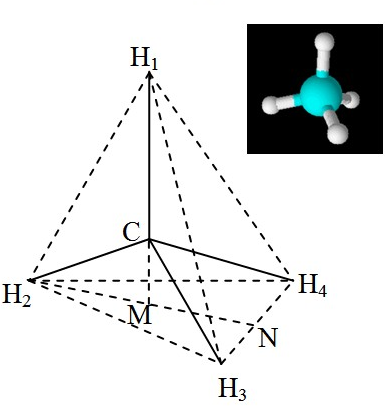
\includegraphics[width=3.35in,height=2.5in,viewport=14 14 250 190,clip]{Tetrahedron.eps}
\caption{\small Arrangement of the secant plane of constant energy in the method of tetrahedrons when $E_0\leqslant E\leqslant E_1$.}
\label{Tetrahedron}
\end{figure}

态密度的一般表达式为,
\begin{equation}
  N_A(E)=\frac1N\sum_{\vec k}A(\vec k)\delta(E-E(\vec k))=\frac{dD_A(E)}{dE}
  \label{eq:solid-198}
\end{equation}
这里
\begin{equation}
  D_A(E)=\frac1N\sum_{\vec k}A(\vec k)\theta(E-E(\vec k))
  \label{eq:solid-199}
\end{equation}
这里$\theta(x)$是Heavyside阶梯函数;$A(\vec k)$是关于矢量$\vec k$的任意函数。对应于式\eqref{eq:solid-197}的三种情况,
电子态密度的表达式分别为,
\begin{enumerate}
\item $E_0\leqslant E\leqslant E_1$
\begin{equation}
  \begin{split}
    N_A(E)=&\frac{|\vec k_{10}[\vec k_{20}\cdot\vec k_{30}]|}\Omega_0\frac{(E-E_0)^2/2}{(E_1-E_0)(E_2-E_0)(E_3-E_0)}\\
    &\cdot\left\{A_0+\left[\frac{A_1-A_0}{E_1-E_0}+\frac{A_2-A_0}{E_2-E_0}+\frac{A_3-A_0}{E_3-E_0}\right](E-E_0)/3\right\}
  \end{split}
  \label{eq:solid-200}
\end{equation}
\item $E_1\leqslant E\leqslant E_2$
\begin{equation}
  \begin{split}
    N_A(E)=&\frac{|\vec k_{10}[\vec k_{20}\cdot\vec k_{30}]|}\Omega_0\left\{\frac{(E-E_0)^2/2}{(E_1-E_0)(E_2-E_0)(E_3-E_0)}\right.\\
    &\cdot\left[A_0+\left(\frac{A_1-A_0}{E_1-E_0}+\frac{A_2-A_0}{E_2-E_0}+\frac{A_3-A_0}{E_3-E_0}\right)(E_3-E_0)/3\right]\\
    &-\frac{(E-E_1)^2/2}{(E_1-E_0)(E_2-E_1)(E_3-E_1)}\\
    &\cdot\left.\left[A_1+\left(\frac{A_1-A_0}{E_1-E_0}+\frac{A_2-A_1}{E_2-E_1}+\frac{A_3-A_1}{E_3-E_1}\right)\frac{(E-E_1)}3\right]\right\}
  \end{split}
  \label{eq:solid-201}
\end{equation}
\item $E_0\leqslant E\leqslant E_1$
\begin{equation}
  \begin{split}
    N_A(E)=&\frac{|\vec k_{10}[\vec k_{20}\cdot\vec k_{30}]|}\Omega_0\frac{(E_3-E)^2/2}{(E_3-E_0)(E_3-E_1)(E_3-E_2)}\\
    &\cdot\left\{A_3-\left[\frac{A_3-A_0}{E_3-E_0}+\frac{A_3-A_1}{E_3-E_1}+\frac{A_3-A_2}{E_3-E_2}\right](E_3-E)/3\right\}
  \end{split}
  \label{eq:solid-202}
\end{equation}
\end{enumerate}

%二次插值方法选择一个大的立方体,%作为工作体积,
%将该立方体分割为小的立方体,立方体的数目为$M^3$,这里$M$取决于计算要求的精度。用通过小立方体体心的三个剖面将每个小立方体分割出27个等价点,$\vec k$点的能量本征值$E(\vec k)$由27个点确定,$E(\vec k)$用小立方体内的一系列$\vec k$点展开到二阶,
%\begin{equation}
%  E(\vec k)=E_0+\vec m\vec k+\vec k\mathbf Q\vec k=\sum_{i=1}^{10}A_ia_i(\vec k)
%  \label{eq:solid-203}
%\end{equation}
%这里$A_i$是展开系数;$a_i(\vec k)$是$\vec k_x$,$\vec k_y$,$\vec k_z$的线性组合到二阶。
晶体的$\vec k$空间积分,除了四面体线性插值外,过去二次插值也是用得比较多的积分方法。关于二次插值的详细介绍,可以参考文献\cite{AP67-15_1971}。无论是线性插值还是二次插值,都各有优劣。对过渡金属,由于其复杂的能带结构,需要很多临界点(高对称性点)的解析解,而且体系的态密度主要由临界点决定,因此对临界点需要高精度的解析计算,但是用线性插值方法很难得到。但是四面体线性插值可以使得整个\textrm{Brillouin}区积分解析完成,因此提高了Fermi能级和Fermi面附近的态密度的计算精度,而这对于金属和导体计算非常重要。此外,线性插值方法也有助于处理非解析临界点(能带交叉点)的情况\cite{PLA28-570_1969,PRB7-891_1973,PRB5-1276_1972}。

能带交叉是\textrm{Brillouin}区积分误差的重要来源,在Brillouin区中接近交叉点的小区域内$|\nabla_{\vec k}E(\vec k)|\simeq0$,会导致$N(E)$的能量奇点的出现,以致于出现不正确的插值计算。%伴随能带交叉产生的另外一个问题是交叉点附近不同可观测物理量的矩阵元的行为。
能带交叉导致矩阵元在交叉点变化剧烈,如果插值点位于这些交叉点上,可能引起更大的误差。理论上,计算精度可以通过增加线性插值的四面体数目%或者二次插值中的参数$M$
来提高,因此插值方法的计算精度主要由布点数目决定。

%有时常将两种方法结合使用,用二次插值计算各参考点的线性插值部分,然后用线性四面体方法计算积分。与之类似的思想就是混合插值,用二次插值得到式\eqref{eq:solid-194}中的梯度
%\begin{equation}
%  \nabla E(\vec k)=\sum_{i=1}^{10}A_i\nabla C_i(\vec k)
%  \label{eq:solid-204}
%\end{equation}
%这里$C_i(\vec k)$式$k_x$,$k_y$,$k_z$的简单解析函数。

\subsection{改进的四面体方法与误差修正}\label{New_Tetrahedron}
四面体方法是更普适的一般方法,除了可用于绝缘体、半导体、金属的期望值计算,还可以计算体系的谱函数,即体系的动态响应性质。但是传统的四面体插值方法为了减少统计四面体的数目,选择在不可约\textrm{Brillouin}区内分割四面体,但这一策略有副作用,由于不可约部分的不规则性,其中的四面体划分几乎不可避免地要人工干预,因此生成四面体的程序化非常困难,\textrm{Bl\"ochl}等改进了线性四面体插值积分方法\cite{PRB49-16223_1994},提出了在已知空间群的情况下,用不可约$\vec k$点快速自动生成四面体的方案,避免了传统方法中分割四面体复杂过程:~
\begin{enumerate}
	\item 利用\textrm{Monkhorst-Pack}方案\cite{PRB13-5188_1976}首先在第一\textrm{Brillouin-zone}内生成等体积的平行六面体网格,并依次用式\eqref{eq:kpoint_Tetra-blochl}的值给每个网格点编号:
\begin{equation}
	N=1+\dfrac{i-i_0}2+(n_1+1)\left[\dfrac{j-j_0}2+(n_2+1)\dfrac{k-k_0}2\right]
	\label{eq:kpoint_Tetra-blochl}
\end{equation}
这里$i,j,k$分别是该$\vec k$点沿倒格矢$\mathbf{b}_i(i=1,2,3)$的序数的二倍,$i_0,j_0,k_0$是\textrm{Monkhorst-Pack}方法中$\Gamma$点许可的偏移量,有偏移则为1,否则为0
	\item 编号之后建立$\vec k$点标识数组,其位置与该位置储存的元素编号值相同,例如,第一个位置存储“$1$”,第二个位置存储“$2$”,依次类推;~
	\item 从第一个位置开始,利用点群的操作元素作用于每个$\vec k$点坐标,并与数组中其余$\vec k$点的坐标进行比较,如果彼此相同且后者的编号大于前者,即将后者的元素编号值改为前者(遍历全部$\vec k$点,可以挑出所有不可约$\vec k$~点:~并且只有当$\vec k_i$为不可约$\vec k$~点时,其编号才与其存储位置相同)。
	\item 为了计算方便,对所有这些不可约$\vec k$点按存储位置的顺序重新编号,即从“$1$”到“$\vec k_{\mathrm{irr}}(\max)$”。并将整个第一\textrm{Brillouin-zone}中的点都用对应的等价不可约点的编号值标记。
	\item 平行六面体中的四面体的自动划分:~
		\begin{itemize}
			\item 假设以下八组坐标代表的点构成平行六面体:
\begin{displaymath}
	\begin{aligned}
		&(l,m,n)\rightarrow 1,&(l+1,m,n)\rightarrow 2\\
		&(l,m+1,n)\rightarrow 3,&(l+1,m+1,n)\rightarrow 4\\
		&(l,m,n+1)\rightarrow 5,&(l+1,m,n+1)\rightarrow 6\\
		&(l,m+1,n+1)\rightarrow 7,&(l+1,m+1,n+1)\rightarrow 8
	\end{aligned}
\end{displaymath}
为了尽量减小插值引起的误差,可以取此平行六面体中最短的体对角线作为等体积的六个四面体的公共对角线,设为$3-6$(图\ref{Fig:Submesh_Tetra}),则可以采用下面6组途径确定这六个四面体的各个顶点:~
\begin{displaymath}
	\begin{aligned}
		1\rightarrow2\rightarrow3\rightarrow6\quad&1\rightarrow3\rightarrow5\rightarrow6\quad&2\rightarrow3\rightarrow4\rightarrow6\\
		3\rightarrow5\rightarrow6\rightarrow7\quad&3\rightarrow4\rightarrow6\rightarrow8\quad&3\rightarrow6\rightarrow7\rightarrow8
	\end{aligned}
\end{displaymath}
		\end{itemize}
\begin{figure}[h!]
\centering
\vspace*{-0.28in}
\includegraphics[height=1.25in,width=3.00in,viewport=0 0 1350 705,clip]{submesh_Tetra.png}
\caption{\small Breakup of a submesh cell into six tetrahedra.}%(与文献\cite{EPJB33-47_2003}图1对比)
\label{Fig:Submesh_Tetra}
\end{figure}
	\item 对每个平行六面体重复上述过程,将第一\textrm{Brillouin-zone}划分为体积相等的若干四面体,每个四面体的顶点可用标识数组中的不可约点编号值标记。
	\item 将每个四面体的四个顶点按编号值升序排列,可以方便地确定等价四面体(顶点编号完全相同的四面体,即为等价四面体)。
\end{enumerate}

这个过程保证了只用不可约点上的信息进行整个第一\textrm{Brillouin}区分割,无须考虑如何划定其不可约部分,
%上述过程可以避免Kleinman所说的计算误差,而且整个过程可以通过程序自动实现而无须人工干预。上述过程可以避免计算误差,
而且整个过程可以通过程序自动实现,无须人工干预。

%仿照特殊点方法,将积分变成不可约$\vec k$点的积分权重求和,
%\begin{equation}
%  \langle X\rangle=\frac1{\Omega_0}\sum_n\int_{\Omega_0}d^3kX_n(\vec k)f(\varepsilon_n(\vec k))=\sum_{jn}X_n(\vec k_j)w_{nj}
%  \label{eq:solid-207}
%\end{equation}
%这里$X_n(\vec k_j)$是可观测量$\langle X\rangle$在不可约$\vec k$点的矩阵元:$X_n(\vec k)=\langle\Psi_n(\vec k)|X|\Psi_n(\vec k)\rangle$;
Brillouin区中任意一点$\vec k$的函数值$X_n(\vec k)$可以通过四面体线性插值得到,
\begin{equation}
  X_n(\vec k)=\sum_jX_n(\vec k_j)w_j(\vec k)
  \label{eq:solid-208}
\end{equation}
$w_j(\vec k)$是四面体插值权重,当积分点在不可约点$\vec k_j$(或者其等价点)上时,插值权重为1,其余不可约点权重为零;在四面体内部,插值权重为线性函数,权重的定义为:
\begin{equation}
	w_{nj}(\vec k)=\frac1{\Omega_0}\int_{\Omega_0}d^3\vec kw_j(\vec k)f(\varepsilon_n(\vec k))
	\label{eq:solid-209}
\end{equation}
对于给定的能带,四面体方法的积分权重也只需计算一次。

\textrm{Bl\"ochl}等在改进四面体方法中专门考虑的积分误差的问题,由此导出了四面体方法对导体和金属积分的修正公式。四面体积分的误差主要有两个来源(如图\ref{Fig:Tetra_error}所示):
	\begin{enumerate}
		\item 四面体内的线性插值引起的误差;~
		\item 临近真实\textrm{Fermi~}面时,四面体内等能面线性插值逼近引入的误差。
	\end{enumerate}
\begin{figure}[h!]
\centering
\vspace*{-0.28in}
\includegraphics[height=1.25in,width=1.25in,viewport=0 0 650 650,clip]{Tetra_error.png}
\caption{\small Schematic representation of the interpolation error due to line interpolation.}%(与文献\cite{EPJB33-47_2003}图1对比)
\label{Fig:Tetra_error}
\end{figure}

对半导体和绝缘体,由于价带被完全填充,通过\textrm{Monkhorst-Pack}布点产生四面体布点方案,只要$\vec k$点足够密集,可以保证在临近\textrm{Fermi}面的线性插值误差完全抵消;~对导体和金属,每个四面体内的线性插值积分误差
\begin{equation}
	\delta\langle X\rangle_T=\int_T\mathrm{d}^3k\left[ X(\vec k)-\bar X(\vec k) \right]
  	\label{eq:solid-Tetra_metal}
\end{equation}
为估计积分误差,假设有被积函数
$$X(\vec k)=a+\sum_ib_ik_i+\frac12\sum_{ij}k_ic_{ij}k_j$$
如果四面体的一个顶点置于原点,其余三个点位于$\vec t_i=(t_{1i},t_{2i},t_{3i})$%(如图\ref{Fig:Tetrahedron}),其中
$i=1,2,3$
%\begin{figure}[h!]
%\centering
%\vspace*{-0.3in}
%\includegraphics[height=1.65in,width=1.70in,viewport=15 15 500 550,clip]{Brillouin-Tetra.eps}
%\caption{\small .}%(与文献\cite{EPJB33-47_2003}图1对比)
%\label{Fig:Tetrahedron}
%\end{figure}
将坐标系$s_i$作线性变换,
$$k_i=\sum_jt_{ij}s_j$$
因此被积函数变换为
$$X(\vec s)=\bar a+\sum_i\bar b_is_i+\frac12\sum_{ij}s_i\bar c_{ij}s_j$$
这里系数$\bar a=a$,$\bar b_i=\sum\limits_jb_jt_{ji}$,$\bar c_{ij}=\sum\limits_{kl}t_{kl}c_{kl}t_{lj}$\\
并且$s_i>0\;i=1,2,3$,$\sum\limits_{i=1}^3s_i\leqslant1$
于是被积函数的线性插的近似值为
$$\bar X(\vec s)=\bar a+\sum_i(\bar b_i+\frac12\bar c_{ii})s_i$$
因此可有积分误差的解析表示为
	\begin{displaymath}
		\begin{aligned}
			\delta\langle X\rangle_T=&\mathrm{det}|t_{ij}|\int_T\mathrm{d}^3s\frac12\left[ \sum_{ij}s_i\bar c_{ij}s_j-\sum_i\bar c_{ii}s_i \right]\\
			=&\frac16\mathrm{det}|t_{ij}|\frac1{40}\left[ \sum_{i\neq j}\bar c_{ij}-3\sum_i\bar c_{ii} \right]
		\end{aligned}
	\end{displaymath}
将$c_{ij}$用被积函数的二阶导数表示,$\frac16\mathrm{det}|t_{ij}|$是四面体体积$V_T$,因此可有
	\begin{displaymath}
		\delta\langle X\rangle_T=V_T\sum_{ij}\left\langle\frac{\partial^2X}{\partial k_i\partial k_j}\right\rangle_TC_{ii}\Delta^2
	\end{displaymath}
这里$\Delta=\sqrt[3]{\mathrm{det}|t|}$
	$$C_{ij}=\frac1{40\Delta^2}\left[ \sum_{l\neq m}t_{il}t_{jm}-3\sum_lt_{ij}t_{jl} \right]$$

对全部占据四面体误差$\delta\langle X\rangle_T$求和,得到插值误差
	\begin{equation}
		\delta\langle X\rangle=\left\langle\sum_{ij}\frac{\partial^2X}{\partial k_i\partial k_j}C_{ii}\right\rangle\Delta^2
		\label{eq:kpoint_Tetra_error}
	\end{equation}
所以四面体积分的误差随$\Delta^2$收敛。

根据\textrm{Green's}积分公式,可将体相积分变成\textrm{Fermi}面的表面积分
	\begin{equation}
		\begin{aligned}
			\delta\langle X\rangle=&\frac1{V_G}\sum_{ij}\langle C_{ij}\rangle\int_{V_G}\mathrm{d}^3k\frac{\partial^2X}{\partial k_i\partial k_j}\Delta^2\\
			=&\frac1{V_G}\sum_{ij}\langle C_{ij}\rangle\oint_{\varepsilon=\varepsilon_{\mathrm F}}\mathrm{d}^2A_i\frac{\partial X}{\partial k_j}\Delta^2
		\end{aligned}
		\label{eq:kpoint_Tetra_surface}
	\end{equation}
因此可有
	\begin{displaymath}
			\delta\langle X\rangle=\frac1{V_G}\sum_{ij}\oint_{\varepsilon=\varepsilon_{\mathrm F}}\mathrm{d}^2A_iC_{ij}\frac{\partial X}{\partial k_j}\Delta^2
	\end{displaymath}
将如下等式
	\begin{displaymath}
		\begin{aligned}
		&\int\mathrm{d}^2A_i=\int\mathrm{d}^2|A|\frac1{\nabla_k\varepsilon}\frac{\partial\varepsilon}{\partial k_i}\\
		&\sum_i\frac{\partial\varepsilon}{\partial k_i}t_{ij}=\varepsilon_{j+1}-\varepsilon_1\\
		&\sum_i\frac{\partial X}{\partial k_i}t_{ij}=X_{j+1}-X_1 
		\end{aligned}
	\end{displaymath}
这里$\varepsilon_i$和$X_i$是四面体顶点的能量和被积函数值,代入最终得到的四面体积分误差校正公式为:~
\begin{equation}
	\begin{aligned}
		\delta\langle X\rangle=&\sum_TD_T(\varepsilon_{\mathrm F})\frac1{40}\left[\sum_{i\neq j}(X_{i+1}-X_1)(\varepsilon_{j+1}-\varepsilon_1)\right.\\
			&-3\left.\sum_i(X_{i+1}-X_1)(\varepsilon_{j+1}-\varepsilon_1)\right]\\
			=&\sum_TD_T(\varepsilon_{\mathrm F})\frac1{40}\sum_{i=1}^4X_i\sum_{j=1}^4(\varepsilon_j-\varepsilon_i) 
	\end{aligned}
	\label{eq:kpoint_Tetra_blochl-error}
\end{equation}
相应地,积分权重校正公式为
\begin{equation}
	\mathrm{d}w_i=\frac{\delta\langle X\rangle}{\delta X_i}=\sum_T\frac1{40}D_T(\varepsilon_{\mathrm F})\sum_{j=1}^4(\varepsilon_j-\varepsilon_i) 
	\label{eq:kpoint_Tetra_blochl-weighterror}
\end{equation}

类似地,考虑等能面线性插值对\textrm{Fermi~}面逼近引起的误差,可有每个四面体的电子数校正:~
\begin{displaymath}
	\delta N_{\mathrm{el},T}=\frac{A_T}{V_G}\sum_{ij}\frac{\partial^2k_{\mathrm F}}{\partial k_i\partial k_j}C_{ij}\Delta^2
\end{displaymath}
这里$A_T$是三角形面积,三角形的形状因子$C_{ij}$表达式为:~
$$C_{ij}=\frac1{24\Delta^2}\left[ \sum_{l\neq m}t_{il}t_{jm}-2\sum_lt_{ij}t_{jl} \right]$$
其中$t_{ij}$是与四面体类似的三角形顶点矢量。%对均匀电子分布,四面体积分误差随$\Delta^3$收敛

%对于导体和金属,传统四面体方法在计算\textrm{Fermi}面附近积分时,都会引入展宽
%四面体积分$W=\dfrac{\mathrm{d}w_i}{\mathrm{d}\varepsilon}$对能量导数对应于“展宽”
%\begin{figure}[h!]
%\centering
%\vspace*{-0.28in}
%\includegraphics[height=1.4in,width=1.55in,viewport=0 0 1000 800,clip]{Tetra_smearing.png}
%%\caption{\small .}%(与文献\cite{EPJB33-47_2003}图1对比)
%\label{Fig:Tetrahedron}
%\ end{figure}
%\begin{itemize}
%\vspace*{-0.1in}
%	\item \textcolor{blue}{四面体方法展宽参数可随能带分布和形状\\
% 	传统展宽方法的展宽系数对所有能带都相同}
% 	\item \textcolor{red}{四面体方法不推荐引入展宽参数}\\
%		\begin{enumerate}
%			\item 展宽计算的总能不满足变分原理,\textrm{Hellmann-Feynman}定理不再满足,\textcolor{red}{不能正确计算导体的受力}
%			\item 四面体能保证态密度计算在\textrm{van Hove}奇点附近出现振荡,引入展宽会破坏这一特征
%		\end{enumerate}
%\end{itemize}

%针对改进后的四面体方法,\textrm{Bl\"ochl}提出了一个形式简单的积分校正公式,
%\begin{equation}
%  \delta\langle X\rangle=\sum_TD_T(\varepsilon_F)\frac1{40}\sum_{j=1}^4X_i\sum_{j=1}^4(\varepsilon_F-\varepsilon_i)
%  \label{eq:solid-205}
%\end{equation}
%相应的积分权重校正为:
%\begin{equation}
%  dw_i=\frac{d\langle X\rangle}{d X_i}=\sum_T\frac1{40}D_T{\varepsilon_F}\sum_{j=1}^4(\varepsilon_F-\varepsilon_i)
%  \label{eq:solid-206}
%\end{equation}
%可以很好的提高对金属的计算结果,而对绝缘体,用改进四面体积分方法用同等数量的布点,可以得到与特殊点方法相同的结果。

%\subsection{晶体的总能量}
%晶体总能量(不包括核的动能)可以分为两部分:一部分是原子核与芯电子组成的离子实能量,这部分能量基本上与晶体结构($\{\vec R\}$)无关,是一个常数,约为$-$$10^3$\,Ry/原子(在固体物理中讨论能量一般沿用Ry单位);另一部分是总能与离子实之差,即离子与价电子的相互作用、离子间的相互作用以及价电子间相互作用,约为$-$10\,Ry/原子。赝势(Pseudo Potential, PP)方法中常把总能量中不变的常数部分(即离子实的能量)设为零。晶体的结合能定义为这部分总能加上核的动能(通常是零点振动能)与孤立原子的能量差。在密度泛函理论中,赝势方法的晶体总能量$E_T$是晶格电子能量$E_{e\textrm{-}e}$与离子实排斥能$E_{N\textrm{-}N}$之和:
%\begin{equation}
%  E_T=E_{e\textrm{-}e}+E_{N\textrm{-}N}=T[\rho]+E_{ext}+E_{Coul}+E_{xc}+E_{N\textrm{-}N}
%  \label{eq:solid-total}
%\end{equation}
%根据Kohn-Sham方程%\eqref{eq:dft-10}
%,动能泛函用单电子能量表示为
%\begin{equation}
%  T[\rho]=\sum_i\langle\psi_i|E_i-V_{KS}|\psi\rangle
%  \label{eq:solid-49}
%\end{equation}
%于是可以得到
%\begin{equation}
%  E_T=\sum_i\varepsilon_i-\frac12\iint d\vec rd\vec r'\dfrac{\rho(\vec r)\rho(\vec r')}{|\vec r-\vec r'|}+\int d\vec r\rho(\vec r)[\varepsilon_{xc}(\vec r)-V_{xc}(\vec r)]+E_{N\textrm{-}N}
%  \label{eq:solid-50}
%\end{equation}
%在计算晶体总能量时,如果利用晶格的周期性,将实空间($\vec r$空间)总能量表示转换到动量空间($\vec k$空间)将使得计算十分便利。
%\begin{equation}
%  E_T=\sum_i\varepsilon_i-\frac{\Omega_0}2\sum_{\vec k\neq0}\rho^{\ast}(\vec k)V_{Coul}(\vec k)+\Omega_0\sum_{\vec k}\rho^{\ast}(\vec k)[\varepsilon_{xc}(\vec k)-V_{xc}(\vec k)]+E_{N\textrm{-}N}
%  \label{eq:solid-51}
%\end{equation}
%这里$V_{Coul}(\vec k)$,$\varepsilon_{xc}(\vec k)$,$V_{xc}(\vec k)$和$\rho(\vec k)$分别是电子间Coulomb相互作用势、电子交换-相关能、交换-相关势和电子密度的Fourier分量,$\Omega_0$为原胞体积。其中电子间Coulomb势的Fourier分量$V_{Coul}(\vec k)$可以从Poisson方程
%\begin{equation}
%  \nabla^2V_{Coul}(\vec r)=-8\pi\rho(\vec r)
%  \label{eq:poisson-r}
%\end{equation}
%用Fourier展开得到
%\begin{equation}
%  V_{Coul}(\vec k)=\dfrac{8\pi\rho(\vec k)}{k^2}
%  \label{eq:poisson-k}
%\end{equation}
%对于交换-相关能和交换相关势,一般根据交换-相关能近似在实空间求得的$\varepsilon_{xc}(\vec r)$和$V_{xc}(\vec r)$后,用Fourier变换到动量空间,得到$\varepsilon_{xc}(\vec k)$和$V_{xc}(\vec k)$。
%
%在实际计算中,需要必要的数学处理,因为离子间Coulomb相互作用能之和:
%$$E_{N\textrm{-}N}=\dfrac12\sum_{\vec r,s}\sideset{}{'}\sum_{\vec R',s'}\dfrac{Z_sZ_{s'}}{|\vec R+\vec{\tau}_s-\vec R'-\vec{\tau}_{s'}|}$$
%这里$Z_s$表示价电子数,$\vec R$表示晶格的格式,$\tau$表示原胞内的原子相对位矢。其求和包含无穷多项;此外$V_{Coul}(\vec k=0)$是发散的;而$V_{ext}$在不考虑其他外场,一般只考虑离子与电子的Coulomb相互作用,
%\begin{equation}
%  \begin{split}
%    V_{ext}(\vec r)=&\sum_{\vec r,s}\dfrac{-2Z_s}{|\vec r-\vec R-\vec r_s|}=\sum_{\vec r,s}\dfrac{-2Z_s}{|\vec r-\vec R-\vec{\tau}_s|} \\
%    =&\sum_{\vec r,s}v_{ext}'(\vec r-\vec R-\vec{\tau}_s)
%  \end{split}
%  \label{eq:solid-52}
%\end{equation}
%它的Fourier分量在$\vec k=0$也是发散的。由于这三项单独都是发散的,但因为整个系统处于电中性,这些发散项相互抵消,是一个常数。因此在解Kohn-Sham方程的时候,可先将$V_{Coul}(\vec k=0)$和$V_{ext}(\vec k=0)$同时置为零,这相当于将势能作一平移,或者说重新定义真空能级,而在总能量计算中补偿这一平移。记这些发散项的和为:
%\begin{equation}
%  \begin{split}
%    \lim\limits_{\vec k\rightarrow0}&\Omega_0\left[\dfrac12V_{Coul}(\vec k)+\sum_sv_{ext}^s(\vec k)\right]\rho(\vec k)+\dfrac12\sum_{\vec R,s}\sideset{}{'}\sum_{\vec R',s'}\dfrac{2Z_sZ_{s'}}{|\vec R+\vec{\tau}_s-\vec R'-\vec{\tau}_{s'}|} \\
%    &=\sum_s\alpha_s\sum_sZ_s+E_{Ewald}
%  \end{split}
%  \label{eq:solid-53}
%\end{equation}
%
%对于形如$Z_s/r$的外场,它的Fourier分量在$\vec k=0$附近展开:$v_{ext}^s(\vec k)=-\dfrac{8\pi Z_s}{\Omega_0k^2}+\alpha_s+o(\vec k)$,同样的展开$\rho(\vec k)$,有$\lim\limits_{\vec k\rightarrow0}\rho(\vec k)=\dfrac{\sum\limits_sZ_s}{\Omega_0}+\beta k^2+o(\vec k)$,代入式\eqref{eq:solid-53},去掉$\vec k$的高次项,有
%\begin{equation}
%  \begin{split}
%    \lim\limits_{\vec k\rightarrow0}&\biggl[\dfrac{\Omega_0}2\dfrac{8\pi\rho^2(\vec k)}{k^2}+\Omega_0\left(\dfrac{-8\pi\sum\limits_sZ_s}{\Omega_0k^2}+\sum_s\alpha_s\right)\rho(\vec k)+\frac12\dfrac{8\pi(\sum\limits_sZ_s)^2}{\Omega_0k^2}\biggr]\\
%    &+\frac12\sum_{\vec R,s}\sideset{}{'}\sum_{\vec R',s'}\dfrac{2Z_sZ_{s'}}{|\vec R+\vec{\tau}_s-\vec R'-\vec{\tau}_{s'}|}-\lim\limits_{\vec k\rightarrow0}\frac12\dfrac{8\pi(\sum\limits_sZ_s)^2}{\Omega_0k^2}\\
%    =&\sum_s\alpha_s\sum_sZ_s+E_{Ewald}
%  \end{split}
%  \label{eq:solid-54}
%\end{equation}
%其中离子间排斥能可用Ewald方法得到\cite{Born-Huang}:
%\begin{equation}
%  \begin{split}
%    E_{Ewald}=&\frac12\sum_{\vec R,s}\sideset{}{'}\sum_{\vec R',s'}\dfrac{2Z_sZ_{s'}}{|\vec R+\vec{\tau}_s-\vec R'-\vec{\tau}_{s'}|}-\lim\limits_{\vec k\rightarrow0}\frac12\dfrac{8\pi(\sum\limits_sZ_s)^2}{\Omega_0k^2} \\
%    =&\frac12\sum_{\vec R,s}\sideset{}{'}\sum_{\vec R',s'}\dfrac{2Z_sZ_{s'}}{|\vec R+\vec{\tau}_s-\vec R'-\vec{\tau}_{s'}|}-\frac1{\Omega_0}\sum_{s,s'}\int d\vec r\frac{Z_sZ_{s'}}r \\
%    =&\sum_{s,s'}Z_sZ_{s'}\left\{\frac{4\pi}{\Omega_0}\sum_{\vec k\neq0}\cos[\vec k\cdot(\vec{\tau}_s-\vec{\tau}_{s'})]\dfrac{e^{-k^2/4\eta^2}}{k^2}\right.\\
%    &-\left.\frac{\pi}{\eta^2\Omega_0}+\frac12\sum_{\vec r}\left.\dfrac{erf(\eta x)}x\right|_{\vec R+\vec{\tau}_s-\vec{\tau}_{s'}\neq0}-\dfrac{2\eta}{\sqrt{\pi}}\delta_{s,s'}\right\}
%  \end{split}
%  \label{eq:solid-55}
%\end{equation}
%这里$erf(x)$是误差函数,参数$\eta$原则上是任意的,如果$\vec r$取得足够多,上述求和是与$\eta$无关的。一般选取$\eta$使得在正格子和倒格子空间收敛得足够快。而$\alpha_s$可根据实际的$v_{ext}^s(\vec r)$得到:
%\begin{equation}
%  \alpha_s=\lim\limits_{\vec k\rightarrow0}\left[v_{ext}^s(\vec k)+\dfrac{8\pi Z_s}{\Omega_0k^2}\right]=\dfrac1{\Omega_0}\int d\vec r\left[v_{ext}^s(\vec r)+\dfrac{2Z_s}r\right]
%  \label{eq:solid-56}
%\end{equation}
%由此得到总能量
%\begin{equation}
%  \begin{split}
%   E_T=&\sum_i\varepsilon_i-\dfrac{\Omega_0}2\sum_{\vec k\neq0}\rho^{\ast}(\vec k)V_{Coul}(\vec k)+\Omega_0\sum_{\vec k}\rho^{\ast}(\vec k)[\varepsilon_{xc}(\vec k)-V_{xc}(\vec k)]\\
%   &+\sum_s\alpha_s\sum_sZ_s+E_{Ewald}
%  \label{eq:solid-57}
%  \end{split}
%\end{equation}
%
%全势方法同样改进了求解Madelung势能的计算方法\cite{JMP22-2433_1981}。MT近似下,WS原胞内中MT球的球心位于$\vec\gamma_{\nu}$,$R_{\nu}$为半径。如果球面上的势能平均为$S_0(R)$,除去球心核电荷以外所有电荷在MT球面上产生的势能平均为:
%\begin{equation}
%  S(R_{\nu})\equiv S_0(R_{\nu})+Z_{\nu}/R_{\nu}
%  \label{eq:solid-79}
%\end{equation}
%则根据$S(R_{\nu})$和球形Dirichlet边值问题\cite{JMP22-2433_1981},球心$\vec\gamma_{\nu}$处的Madelung势(因为要求的Madelung势位于球心,只有$l=0$部分对此有贡献,故只需考虑$S(R_{\nu})$的球形平均部分)为\cite{PRB26-4571_1982}:
%\begin{equation}
%  \begin{split}
%   V_M(\vec\gamma_{\nu})&=\frac1{R_{\nu}}[R_{\nu}S_0(R_{\nu})+Z_{\nu}-Q_{\nu}]+\sqrt{4\pi}\int_0^{R_{\nu}}drr\rho_{00}(r_{\nu})\\
%   &=\frac1{R_{\nu}}[R_{\nu}S_0(R_{\nu})+Z_{\nu}-Q_{\nu}]+\bigg\langle\frac1r\rho(\vec r)\bigg\rangle_{\nu}
%  \end{split}
%   \label{eq:Madelung}
%\end{equation}
%其中$Q_{\nu}$表示MT球内的电子电荷之和。$\rho(\vec r)$是MT球内的电荷密度,可以用球谐函数表示为
%\begin{equation}
%  \rho(\vec r_{\nu})=\sum_{lm}\rho_{lm}(r_{\nu})Y_{lm}(\hat r_{\nu})
%  \label{eq:solid-80}
%\end{equation}
%类似地,WS原胞内的总能量可以表示为:
%\begin{equation}
%  \begin{split}
%   E_T=&\sum_i\varepsilon_i-\frac12\int_{\Omega_0}\rho(\vec r)[V_c(\vec r)+2\mu_{xc}(\vec r)]d\vec r-\frac12\sum_{\nu}Z_{\nu}V_M(\vec\gamma_{\nu})+E_{xc}[\rho] \\
%   =&\sum_i\varepsilon_i-\frac12\left(\int_{\Omega_0}\rho(\vec r)V_c(\vec r)d\vec r+\sum_{\nu}Z_{\nu}\bigg\langle\frac1r\rho(\vec r)\bigg\rangle_{\nu}\right)-\int_{\Omega_0}\rho(\vec r)\mu_{xc}(\vec r)d\vec r\\
%   &-\frac12\sum_{\nu}\frac{Z_{\nu}}{R_{\nu}}[R_{\nu}S_0(R_{\nu})+Z_{\nu}-Q_{\nu}]+E_{xc}[\rho]
%  \end{split}
%  \label{eq:solid-81}
%\end{equation}
%这里$V_c(\vec r)=\int\dfrac{\rho(\vec r')}{|\vec e-\vec r'|}d\vec r'-\sum\limits_{\alpha}\dfrac{Z_{\alpha}}{|\vec r-\vec r_{\alpha}|}$。总能量写成这样的形式,原子核位置的Coulomb势奇点可以排除。将势能和电荷密度在各原子核附近作球谐展开,在原子核附近,有
%\begin{displaymath}
%  \begin{split}
%    &\int_{\Omega_0}\rho(\vec r)V_c(\vec r)d\vec r+Z{\nu}\sqrt{4\pi}\int_0^{R_{\nu}}drr^2\frac{\rho_{00}(r)}r\\
%    =&\sqrt{4\pi}\int_{\Omega_0}drr^2\rho_{00}(\vec r)\left(V_{00}(r)Y_{00}(\hat r)+\frac{Z_{\nu}}r\right)+\sum_{lm>0}\int drr^2\rho_{lm}(r)V_{lm}(r)
%  \end{split}
%\end{displaymath}
%Coulomb势的奇点只出现在$V_{00}(r)$中,将$V_{00}(r)$写成核的点电荷势与源于电子的平滑势两部分之和,有
%$$V_{00}(r)=-\sqrt{4\pi}\frac{Z_{\nu}}r+\hat V_{00}(r)$$
%有必要指出的是,通过这样的方式,可以将总能量中的奇点排除,但是单独每一项在原子核位置能量仍然是发散的。
%
%如果采用标准的LDA近似,式\eqref{eq:solid-81}交换-相关能可以写成:
%\begin{equation}
%  E_{xc}[\rho]\approx\int_{\Omega_0}\rho(\vec r)\varepsilon_{xc}(\vec r)d\vec r
%  \label{eq:solid-82}
%\end{equation}
%
%一般地,总能量计算在动量空间中完成。在MT近似下,间隙区的电荷密度用平面展开,有
%$$\rho(\vec r)=\sum_{\vec G}e^{i\vec G\cdot\vec r},\quad \vec r\in\mathrm{Interstitial}$$
%在MT球内,电荷密度用球谐函数展开,在动量空间中的展开形式为:
%$$\bar\rho_{lm}(r_{\nu})=4\pi i^l\sum_{\vec G}\rho(\vec G)e^{i\vec G\cdot\vec{\gamma}_{\nu}}j_l(Gr_{\nu})Y_{lm}^{\ast}(\vec G)$$
%于是,WS原胞内的晶体总能量可以写成:
%\begin{equation}
%  \begin{split}
%  E=&\sum_i\varepsilon_i-\sum_{\vec G}\Omega_0\rho(\vec G)-\frac12\sum_{\nu}\dfrac{Z_{\nu}}{R_{\nu}}[Z_{\nu}-Q_{\nu}+R_{\nu}S_0(R_{\nu})]\\
%  &-\sum_{\nu}\sum_{lm}\int_0^{R_{\nu}}drr^2\left[\rho_{lm}(r_{\nu})\left(\tilde V_{lm}^{\ast}(r_{\nu})\dfrac{\sqrt{4\pi}}{2r_{\nu}}Z_{\nu}\delta_{l0}\right)-\bar\rho_{lm}(\vec r_{\nu})\bar V_{lm}^{\ast}(\vec r_{\nu})\right]
%  \end{split}
%  \label{eq:solid-83}
%\end{equation}
%这里$\tilde V(\vec r)$和$\bar V_{lm}(\vec r)$根据下式计算:
%$$\tilde V(\vec r)=\frac12V_c(\vec r)-\varepsilon_{xc}(\vec r)+\mu_{xc}(\vec r)$$

\chapter{LDA+$U$和GW近似}
\section{LDA+$U$方法}
由于带电粒子间的\textrm{Coulomb}作用,运动中的电子间必然存在相互排斥。但是传统的能带理论为简化问题,处理电子系统时采用的是单粒子图像(平均场近似)。基于\textrm{DFT}理论虽然通过引入电子交换-相关泛函来修正电子间的相互作用,但由于精确的交换-相关泛函的形式未知,所以如何更好地描述电子关联(electron correlation)是伴随着\textrm{DFT}与生俱来的重要问题。\textrm{Perdew}的研究表明LDA近似和精确密度泛函方法的重要差别\cite{PRL49-1691_1982}:~尽管交换-相关泛函的精确形式不知,但总能量泛函对电子数的依赖$E(N)$应该具有折线特征(见图\ref{exact-DFT}):~
	\begin{displaymath}
		\dfrac{\Delta E}{\Delta N}=\left\{
		\begin{aligned}
			E(M)-E(M-1)|_{\mathrm{left}}\qquad M-1<N<M\\
			E(M+1)-E(M)|_{\mathrm{right}}\qquad M<N<M+1 
		\end{aligned}\right.
	\end{displaymath}
换句话说,电子数$N$改变整数值的时候,精确的单电子势$V(\vec r)=\dfrac{\delta E}{\delta n(\vec r)}$的改变应该是不连续的。而LDA近似下,显然势能是电子数$N$的连续函数。因为不具备势能随电子数变化不连续的特征,所以LDA方法在描述含有{\textit d}\,或{\textit f}\,电子的过渡金属和稀土元素化合物体系时常常失效。

\begin{figure}[h!]
\centering
\vspace*{-0.4in}
\includegraphics[height=2.4in,width=2.8in,viewport=0 0 1000 880,clip]{exact-DFT.png}
\caption{\small \textrm{The dependence of the total energy on the number of electron is a series of straight-line segments.}}%(与文献\cite{EPJB33-47_2003}图1对比)
\label{exact-DFT}
\end{figure}

Gunnarsson和Schonhammer\cite{PRL56-1968_1986}证明,单电子势的不连续对能带的带隙有很大的贡献。LDA近似的另一个不足还在于,LDA计算得到的轨道能量(定义为能量$E$对轨道占据数$n_i$的导数,即$\varepsilon_i=\partial E/\partial n_i$),不满足\textrm{Koopmans}定理,与实验或者严格计算得到的轨道能量差别很大。但是另一方面,LDA方法得到的总能量一般与实验结果符合的较好。一个典型的例子就是\textrm{H}原子的计算,LDA计算的轨道能为$-0.54\,\mathrm{Ry}$(实际结果为$-1.0\,\mathrm{Ry}$),总能量($-0.976\,\mathrm{Ry}$)则非常接近$-1.0\,\mathrm{Ry}$\cite{PRB37-9919_1988}。文献\inlinecite{PRB44-943_1991}提出通过对LDA势加入轨道校正克服LDA方法的不足(称为LDA+$U$方法)。LDA+$U$方法与\textrm{Andersen}掺杂模型\cite{PR124-41_1961}思想相同,对局域的{\textit d}\,或{\textit f}\,电子,采用模型Hamiltonian方法考虑$d$-$d$或$f$-$f$间相互作用(定域Coulomb相互作用$U$),离域的{\textit s}\,和{\textit p}\,电子的运动用LDA近似描述。

在文献\inlinecite{Herring}中,\textrm{Herring}讨论了$U$值的物理意义:~含有$n$个3{\textit d}\,电子的原子中,如果定义两个原子间转移一个{\textit d}\,电子,即
$$2(d^n)\rightarrow d^{n+1}+d^{n-1}$$
能量的改变为$U$
$$U=E(d^{n+1})+E(d^{n-1})-2E(d^n)$$
在\textrm{DFT}框架下,\textrm{L(S)DA}是弱耦合的平均场(\textrm{mean-filed, MF})理论,对于{\textit d}\,电子数目发生变化的原子/离子体系,$d$-$d$电子间的相互作用可以表示为$E=UN(N-1)/2$\cite{PRB48-16929_1993},将总能量中扣除LDA的$d$-$d$电子相互作用,再加上局域的电子间相互作用,可有
\begin{equation}
  E=E_{LDA}-UN(N-1)/2+\frac12U\sum_{i\neq j}n_in_j
  \label{eq:solid-251}
\end{equation}
由式\eqref{eq:solid-251}对轨道占据数$n_i$求导得轨道能
\begin{equation}
  \varepsilon_i=\frac{\partial E}{\partial n_i}=E_{LDA}+U(\frac12-n_i)
  \label{eq:solid-252}
\end{equation}
\begin{figure}[h!]
\centering
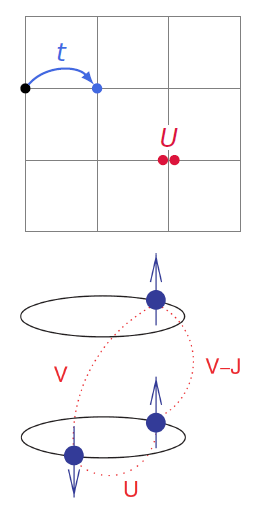
\includegraphics[height=1.35in,width=0.92in,viewport=1 1 240 375,clip]{LDA_U-1.png}
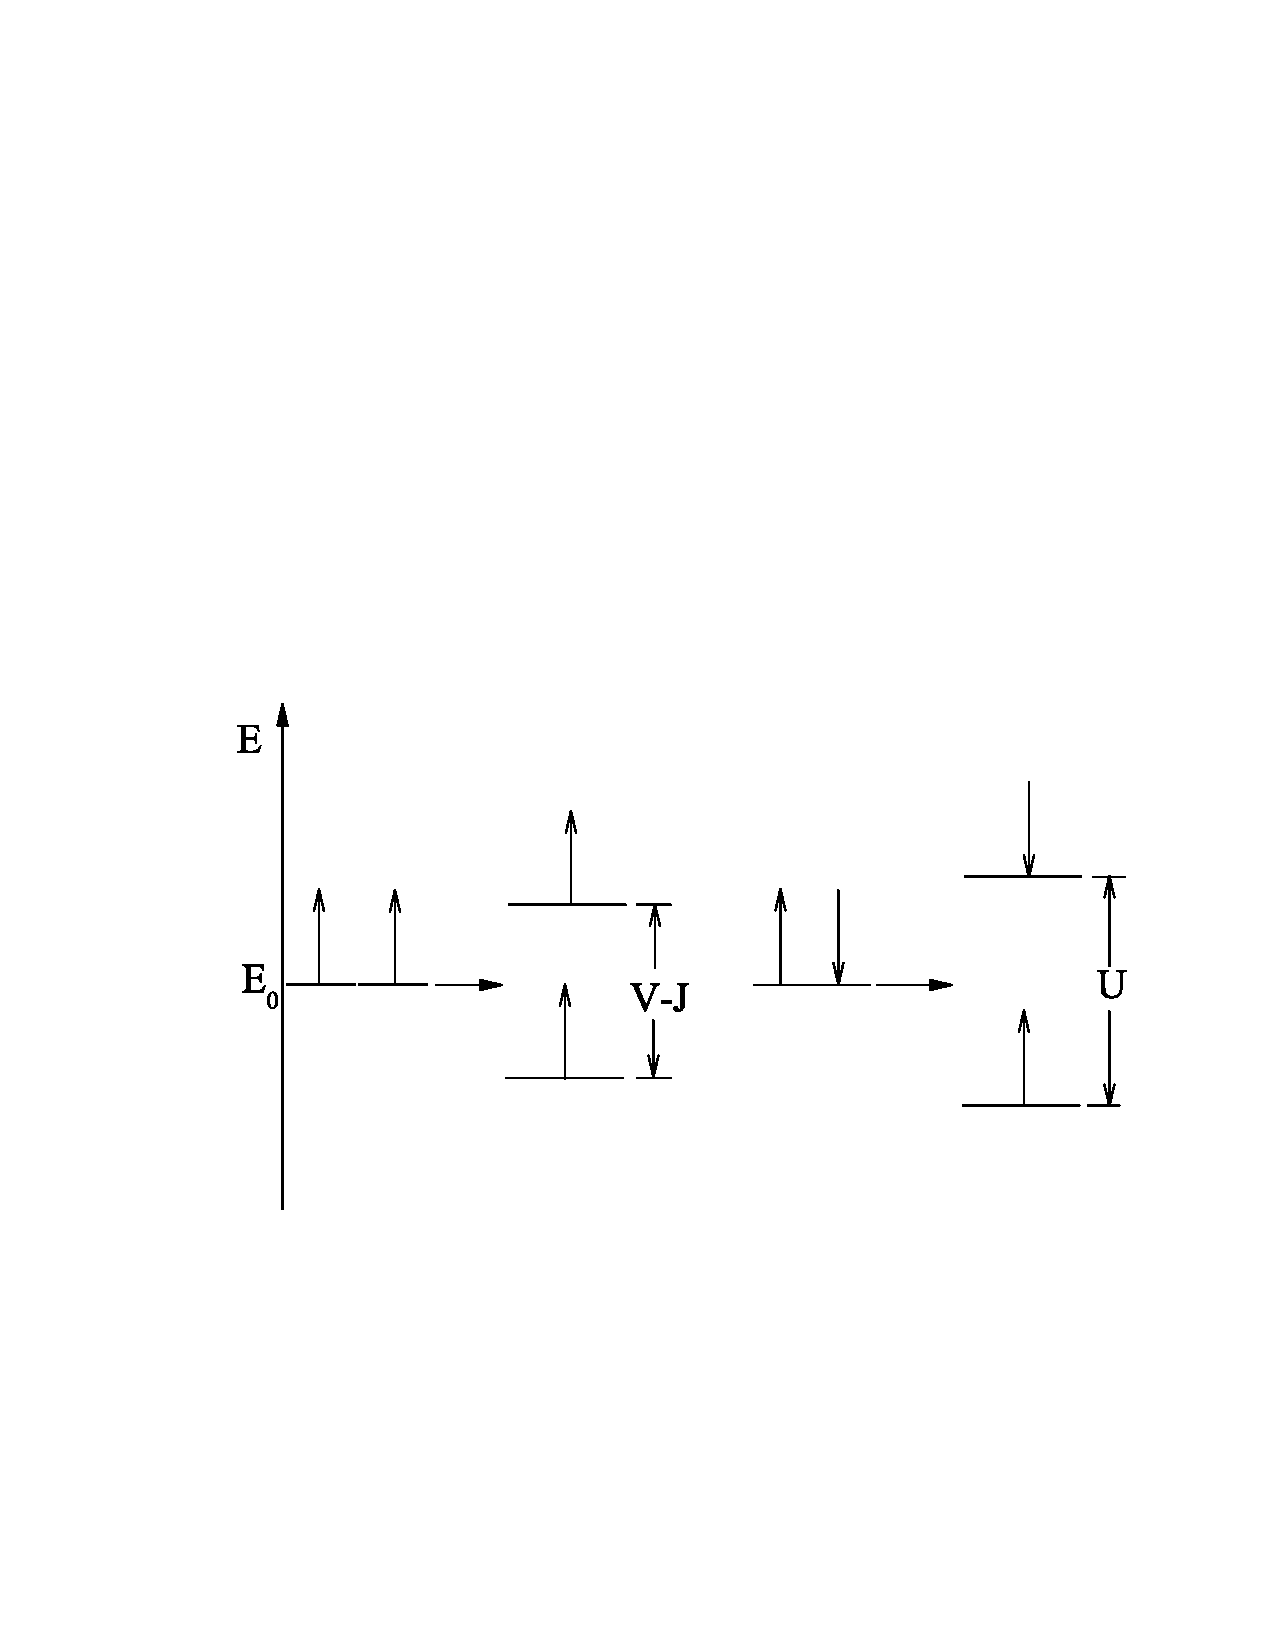
\includegraphics[height=1.35in,width=2.32in,viewport=110 210 545 455,clip]{LDA_U.pdf}
\caption{\small \textrm{The meaning of $U$, when the Coulomb-interaction of each electron is taken into account.}}%(与文献\cite{EPJB33-47_2003}图1对比)
\label{U_means}
\end{figure}
该式将占据态轨道($n_i$=1)和非占据态轨道($n_i$=0)的LDA轨道能分别移动-$U$/2和+$U$/2,由此得到的轨道相关势[$V_i(\vec r)=\delta E/\delta n_i(\vec r)$]为
\begin{equation}
  V_i(\vec r)=V_{LDA}(\vec r)+U(\frac12-n_i)
  \label{eq:solid-253}
\end{equation}
式\eqref{eq:solid-253}表明\textrm{LDA}+$U$,通过简单引入唯象参数$U$,保留了精确密度泛函理论的单电子势能所必需的不连续特征。图\ref{U_means}给出了参数$U$的物理含义示意:~$U$表示位于同一格点上电子间的排斥相互作用。

式\eqref{eq:solid-251}没有考虑相同自旋电子的交换作用。设自旋$\sigma$的{\textit d}-{\textit d}\,电子间交换参数为{\textit J}\,,则{\textit N}\,电子的LDA近似下{\textit d}-{\textit d}\,相互作用为$UN(N-1)/2-JN(N-2)/4$。

如果进一步考虑Coulomb势和交换势的非球形部分的贡献(与{\textit d}\,轨道的$m$和$m^{\prime}$相关部分),引入矩阵元$U_{mm^{\prime}}$和$J_{mm^{\prime}}$,有
\begin{equation}
  U_{mm^{\prime}}=\sum_ka_kF^k
  \label{eq:solid-210}
\end{equation}
\begin{equation}
  J_{mm^{\prime}}=\sum_kb_kJ^k
  \label{eq:solid-211}
\end{equation}
\begin{equation}
  a_k=\frac{4\pi}{2k+1}\sum_{q=-k}^k\langle lm|Y_{kq}|lm\rangle\langle lm|Y_{kq}^{\ast}|lm^{\prime}\rangle
  \label{eq:solid-212}
\end{equation}
\begin{equation}
  b_k=\frac{4\pi}{2k+1}\sum_{q=-k}^k|\langle lm|Y_{kq}|lm^{\prime}\rangle|^2
  \label{eq:solid-213}
\end{equation}
这里$F^k$是Slater积分,$\langle lm|Y_{kq}|lm^{\prime}\rangle$是三个球谐函数$Y_{lm}$的乘积的积分。

由此得到的总能量为
\begin{equation}
  \begin{split}
	  E=&E_{\mathrm{LDA}}-[UN(N-1)/2-JN(N-2)/4]\\
  &+\frac12\sum_{m,m^{\prime},\sigma}U_{mm^{\prime}}n_{m\sigma}n_{m^{\prime}\sigma}\\
  &+\frac12\sum_{m\neq m^{\prime},m^{\prime},\sigma}(U_{mm^{\prime}}-J_{mm^{\prime}})n_{m\sigma}n_{m^{\prime}\sigma}
  \end{split}
  \label{eq:solid-214}
\end{equation}
式\eqref{eq:solid-214}应占据数$n_{m\sigma}$求导,得到轨道相关的单电子势能
\begin{equation}
  \begin{split}
	  V_{m\sigma}(\vec r)=&V_{\mathrm{LDA}}(\vec r)+\sum_{m^{\prime}}(U_{mm^{\prime}}-U_{\mathrm{eff}})n_{m-\sigma}\\
	  &\sum_{m\neq m^{\prime}}(U_{mm^{\prime}}-J{mm^{\prime}}-U_{\mathrm{eff}})n_{m\sigma}+U_{eff}\left(\frac12-n_{m\sigma}\right)-\frac12J
  \end{split}
  \label{eq:solid-215}
\end{equation}
这里$U_{\mathrm{eff}}=U-J/2$。

为了计算矩阵元$U_{mm^{\prime}}$和$J_{mm^{\prime}}$,必须知道Slater积分$F^k$(对{\it d}\,电子是$F^0$,$F^2$和$F^4$)。文献\cite{PRB43-7570_1991}用超晶胞近似(supercell approximation)给出Coulomb参数$U$,和$F^0$相等,将矩阵元$U_{mm^{\prime}}$和$(U_{mm^{\prime}}-J_{mm^{\prime}})$对所有$mm^{\prime}$求平均,可以得到$U$和$(U-J)$,根据Clebsch-Gordan系数性质,有平均值为
\begin{equation}
  U=\frac1{(2l+1)^2}\sum_{mm^{\prime}}U_{mm^{\prime}}=F^0
  \label{eq:solid-216}
\end{equation}
\begin{equation}
  U-J=\frac1{2l(2l+1)}\sum_{mm^{\prime}}(U_{mm^{\prime}}-J_{mm^{\prime}})=F^0-(F^2+F^4)
  \label{eq:solid-217}
\end{equation}
\begin{equation}
  J=(F^2=F^4)/4
  \label{eq:solid-218}
\end{equation}
为了由$U$和$J$得到所有的Slater积分,只需要知道$F^4/F^2$\cite{PRB42-5459_1990}。

LDA+$U$方法最重要的特征是具备了单电子势的不连续性。计算表明LDA+$U$方法对含有定域强Coulomb相互作用的体系是可靠的\cite{PRB48-16929_1993,JPCS56-1521_1995,EPL36-551_1996}。无论对含有近芯层的局域4{\textit f}\,电子的稀土金属离子还是对过渡金属的氧化物(金属的3{\textit d}\,电子与氧原子2{\textit p}\,轨道有很强的相互作用)体系都有效。尽管LDA+$U$方法只是通过参数$U$唯象地考虑电子间的关联效应,并未突破平均场近似框架,因此不足以描述金属-绝缘体的\textrm{Mott}转变和具有强关联的金属。但对诸如FeSi和LaCaO$_3$这类化合物,LDA+$U$已经能够给出有关于金属-绝缘体转变的有用信息\cite{JPCM9-767_1997}。甚至对含有5{\textit f}\,电子的化合物的研究也取得一定的成功\cite{PRB54-R3706_1996}。

\section{电子激发与GW近似}
Landau的Fermi液体理论是研究群体激发和多体Fermi子体系物理性质的重要方法\cite{Landau}。Fermi液体的特征是准粒子分布$\varepsilon=\varepsilon(\vec k)$由体系总能量$E$对分布函数的变分,即
\begin{equation}
  \frac{\delta E}{\delta n(\vec k)}=\varepsilon(\vec k)
  \label{eq:solid-219}
\end{equation}
关联函数$f(\vec k,\vec k^{\prime})$由准粒子能量对整个$\vec k$空间粒子分布变分得到
\begin{equation}
  \frac{\delta\varepsilon(\vec k)}{\delta n(\vec k^{\prime})}=\frac{\delta^2E}{\delta n(\vec k)\delta n(\vec k^{\prime})}=f(\vec k,\vec k^{\prime})
  \label{eq:solid-220}
\end{equation}
考虑准粒子间相互作用,体系激发能记作
\begin{equation}
  W=\sum_{\vec k}\varepsilon(\vec k)\delta n(\vec k)+\frac12\sum_{\vec k}\sum_{\vec k^{\prime}}f(\vec k,\vec k^{\prime})\delta n(\vec k)\delta(\vec k^{\prime})
  \label{eq:solid-221}
\end{equation}

Green函数是研究Fermi液体的重要数学工具。对宏观体系,Green函数定义为\cite{Lifshitz}
\begin{equation}
	\tilde G(x,x^{\prime})=-\mathrm{i}\langle T\hat\Psi(x)\hat\Psi^{\ast}(x^{\prime})\rangle
  \label{eq:solid-222}
\end{equation}
这里$x$表示时间$t$和位置$\vec r$,$\langle\cdots\rangle$表示对体系基态求平均,$T$表示按时间先后乘积算符。$\hat\Psi$是Heisenberg算符,对式\eqref{eq:solid-222}进行Fourier变换,得到以$\vec r$,$E$为表象的Green函数$\tilde G(\vec r,\vec r^{\prime};E)$是Dyson方程\cite{Lifshitz}
\begin{equation}
	(\dfrac12\nabla^2+E)\tilde G(\vec r,\vec r^{\prime};E)-\int\mathrm{d}\vec r^{\prime\prime}\Sigma(\vec r,\vec r^{\prime\prime};E)\tilde G(\vec r^{\prime\prime},\vec r^{\prime};E)=\delta(\vec r-\vec r^{\prime})
  \label{eq:solid-223}
\end{equation}
的解。这里$\Sigma(\vec r,\vec r^{\prime};E)$是描述交换和相关效应的质量或自能算符,这是个与能量有关的非定域的非-Hermitian算符,考虑到粒子与体系中其他粒子的相互作用。晶体中的质量具有平移对称性,
\begin{equation}
  \Sigma(\vec r+\vec a,\vec r+\vec a;E)=\Sigma(\vec r,\vec r^{\prime};E),
  \label{eq:solid:224}
\end{equation}
这里$\vec a$是晶体平移格矢。

临近Green函数的极点,式\eqref{eq:solid-223}右面的$\delta$函数为0,所得积分-微分方程的本征值确定体系激发能谱\cite{Lifshitz,PR145-561_1966}
\begin{equation}
	-\delta^2\Phi_{\vec k}(\vec r,E)+\int\mathrm{d}\vec r^{\prime}\Sigma(\vec r,\vec r^{\prime};E)\Phi_{\vec k}(\vec r^{\prime},E)=\varepsilon_{\vec k}\Phi_{\vec k}(\vec r,E) 
  \label{eq:solid-225}
\end{equation}
这里函数$\Phi_{\vec k}(\vec r,E)$类似于周期场中的单电子Bloch波函数。对金属中的Fermi电子液体中用式\eqref{eq:solid-225}替代一般Schr\"odinger方程。与一般的Schr\"odinger方程不同,式\eqref{eq:solid-225}的能量本征值是复数,因为质量算符$\Sigma(\vec r,\vec r^{\prime};E)$是复数。

由式(\ref{eq:solid-223},\ref{eq:solid-225})得到Green函数
\begin{equation}
	\tilde G(\vec r,\vec r^{\prime};E)=\sum_{\vec k}\frac{\Phi_{\vec k}(\vec r,E)\Phi_{\vec k}^{\ast}(\vec r^{\prime},E)}{E-\varepsilon_{\vec k}(E)+\mathrm{i}0\mathrm{sgn}E}
  \label{eq:solid-226}
\end{equation}
$\varepsilon_{\vec k}(E)$是体系中加入一个粒子引起的能量改变。如果将单个准粒子改变引起得能量变化$\varepsilon_{\vec k}(E)$定义为式\eqref{eq:solid-219}中的准粒子能量,对临近Fermi面的态,函数$\tilde G(\vec r,\vec r^{\prime};E)$在$E=\varepsilon_{\vec k}(E)$有极值。因此Green函数极值确定了多Fermi子体系的元激发能谱。一般说,因为和其他粒子相互作用,准粒子能量为复数。复数能量使得体系激发态的寿命有限$(\tau\sim1/|\mathrm{Im}\varepsilon|)$\cite{Landau-Lifshitz}。能量宽度由$\mathrm{Im}\varepsilon$确定。

%临近Fermi能级,$\mathrm{Im}\varepsilon_{\vec k}(E)\rightarrow0$,相应的$\mathrm{Im}\Sigma\rightarrow0$,于是解方程\eqref{eq:solid-225}得到$\mathrm{Re}\varepsilon_{\vec k}(E)$和实数形式的$\Sigma(\vec r,\vec r^{\prime};E)$和$\epsilon_{\vec k}(E)$。

根据Hohenberg-Kohn定理,本征值$\Sigma(\vec r,\vec r^{\prime};E)$由体系基态确定,它也是电子密度的函数。Sham和Kohn建议可用局域电子密度近似表示$\Sigma(\vec r,\vec r^{\prime};E)$\cite{PR145-561_1966}:
\begin{equation}
  \Sigma(\vec r,\vec r^{\prime};E)=V_C(\vec r)\delta(\vec r-\vec r^{\prime})+\Sigma_0(\vec r-\vec r^{\prime};E-V_C(\vec r_0);\rho(\vec r_0))
  \label{eq:solid-227}
\end{equation}
这里$\Sigma_0$是密度为$\rho$的无相互作用电子气的本征能量,$V_C(\vec r_0)$是位于$\vec r_0=(\vec r+\vec r^{\prime})/2$的静电Coulomb势。此外式\eqref{eq:solid-227}已将能量$\Sigma$中的局域部分以Hartree势的形式分离出来,因此可以利用$\Sigma_0$的短程效应。

对本征函数$\Phi_{\vec k}$作近似
$$\Phi_{\vec k}(\vec r,E)=A(\vec k)\exp[\mathrm{i}\vec p(\vec r)\vec r]$$
并认为$A$和电子动量与$\vec r$无关,将式\eqref{eq:solid-225}称为类似Kohn-Sham方程的表达式\cite{JPC4-2064_1971},
\begin{equation}
  [-\dfrac12\nabla^2+V_C(\vec r)+\Sigma_{xc}(\rho(\vec r),E)]\Phi_{\vec k}(\vec r,E)=\varepsilon_{\vec k}(\vec r,E)
  \label{eq:solid-228}
\end{equation}
若$E=\mu$,$\Sigma_{xc}(\rho(\vec r),\mu)\equiv\mu_{xc}(\rho(\vec r))$我们因此得到符合局域密度近似的DFT方程,两者的交换-相关势$\mu_{xc}$是相同的。因此对于低激发能,可以使用近似$\Sigma_{xc}(\rho(\vec r),E)\simeq\mu_{xc}$,此结果对应于忽略准粒子间的相互作用,即Landau函数$f(\vec k,\vec k^{\prime})=0$。

因此基于DFT的能带计算,如果充分考虑交换-相关效应,可以计算多电子体系的元激发能量。注意,采用单电子近似,要求能带比较宽,即中心位于不同格点的波函数有较大的重叠,电子间相互作用不是很强。

Hedin和Lundqvist详细回顾了用Green函数技术解决电子相关的问题\cite{Hedin-Lundqvist}。在单粒子近似下的Green函数,准粒子与谱函数的峰联系在一起。如果峰足够尖锐,表明存在一个明确的准粒子能量,对一般的非均匀体系,准粒子能量和波函数可以通过解Dyson方程\eqref{eq:solid-225}求得。对于准粒子问题,核心问题是对自能算符$\Sigma(\vec r,\vec r^{\prime};E)$的足够好的近似。常用的方法是GW近似\cite{PR139-A796_1965},自能用屏蔽相互作用$W$计算到最低阶。
\begin{equation}
	\Sigma(\vec r,\vec r^{\prime};E)=\dfrac{\mathrm{i}}{2\pi}\int_{-\infty}^{\infty}\mathrm{d}E^{\prime}\tilde G(\vec r,\vec r^{\prime};E+E^{\prime})W(\vec r,\vec r^{\prime};E^{\prime})
  \label{eq:solid-229}
\end{equation}
Green函数$\tilde G$由准粒子的波函数和能量表示,屏蔽Coulomb作用$W$
\begin{equation}
	W(\vec r,\vec r^{\prime};E)=\frac1{\Omega}\int\mathrm{d}^3r^{\prime\prime}\varepsilon^{-1}(\vec r,\vec r^{\prime\prime};E)V(\vec r^{\prime\prime}-\vec r^{\prime})
  \label{eq:solid-230}
\end{equation}
这里$V$是未屏蔽的Coulomb势,$\varepsilon^{-1}$是介电函数矩阵的逆阵,
\begin{equation}
	\varepsilon^{-1}(\vec r,\vec r^{\prime};E)=\delta(\vec r-\vec r^{\prime})+\int\mathrm{d}^3r^{\prime\prime}V(\vec r^{\prime}-\vec r^{\prime\prime})P(\vec r^{\prime\prime},\vec r^{\prime};E)
  \label{eq:solid-231}
\end{equation}
这里$P$是完全响应函数,于是
\begin{equation}
  W(\vec r,\vec r^{\prime};E)=V(\vec r-\vec r^{\prime})+W_c(\vec r,\vec r^{\prime};E)
  \label{eq:solid-232}
\end{equation}
这里
\begin{equation}
	W_c(\vec r,\vec r;E)=\int\mathrm{d}^3r_1d^3r_2V(\vec r^{\prime}-\vec r_1)P(\vec r_1,\vec r_2;E)V(\vec r_2-\vec r^{\prime})
  \label{eq:solid-233}
\end{equation}
Green函数可以写成谱表示
\begin{equation}
	G(\vec r,\vec r^{\prime};E)=\int_{-\infty}^{\mu}\mathrm{d}E^{\prime}\frac{A(\vec r,\vec r^{\prime};E^{\prime})}{E-E^{\prime}-i\delta}+\int_{\mu}^{\infty}\mathrm{d}E^{\prime}\frac{A(\vec r,\vec r^{\prime};E^{\prime})}{E-E^{\prime}+i\delta}
  \label{eq:solid-234}
\end{equation}
这里$A(\vec r,\vec r^{\prime};E)=-\frac1{\pi}\mathrm{Im}G(\vec r,\vec r^{\prime};E)\mathrm{sgn}(E-\mu)$

实际计算中,取零阶Green函数,有
\begin{equation}
  A(\vec r,\vec r^{\prime};E)=\sum_{kn}\psi_{kn}(\vec r)\psi_{kn}^{\ast}(\vec r^{\prime})\delta(E-E_{kn})
  \label{eq:solid-235}
\end{equation}
于是自能可以写成
\begin{equation}
  \Sigma(\vec r,\vec r^{\prime};E)=\Sigma_x(\vec r,\vec r^{\prime})+\Sigma_c(\vec r,\vec r^{\prime};E)
  \label{eq:solid-236}
\end{equation}
这里$\Sigma_x$是净的交换势,
\begin{equation}
	\Sigma_x(\vec r,\vec r^{\prime})=-\sum_{kn}^{\mathrm{occ}}\psi_{kn}(\vec r)\psi_{kn}^{\ast}(\vec r^{\prime})V(\vec r-\vec r^{\prime})
  \label{eq:solid-254}
\end{equation}
$E_c$自能的相关部分,
\begin{equation}
  \begin{split}
	  \Sigma_c(\vec r,\vec r^{\prime};E)=&\sum_{kn}^{\mathrm{occ}}\psi_{kn}(\vec r)\psi_{kn}^{\ast}(\vec r^{\prime})W_c^-(\vec r,\vec r^{\prime};E-E_{kn})\\
	  &+\sum_{kn}^{\mathrm{occ}}\psi_{kn}(\vec r)\psi_{\vec r}^{\ast}(\vec r^{\prime})W_c^+(\vec r,\vec r^{\prime};E-E_{kn})
  \end{split}
  \label{eq:solid-237}
\end{equation}
其中$W_c^{\pm}(\vec r,\vec r^{\prime};E)=\dfrac{\mathrm{i}}{2\pi}\int_{-\infty}^{+\infty}\mathrm{d}E^{\prime}\frac{W_c(\vec r,\vec r^{\prime};E^{\prime})}{E+E^{\prime}\pm i\delta}$。于是$\Sigma(\vec r,\vec r^{\prime};E)$可以记作\cite{JPCM9-767_1997},
\begin{displaymath}
  \Sigma(\vec r,\vec r^{\prime};E)=-\sum_{kn}\psi_{kn}(\vec r)\psi_{kn}^{\ast}(\vec r^{\prime})W_0(\vec r,\vec r^{\prime};E-E_{kn})
\end{displaymath}
其中
\begin{displaymath}
  \begin{aligned}
    W_0(\vec r,\vec r^{\prime};E-E_{kn})\equiv&[V(\vec r-\vec r^{\prime})-W_c^-(\vec r,\vec r^{\prime};E-E_{kn})]\theta(\mu-E_{kn})\\
    &-W_c^+(\vec r,\vec r^{\prime};E-E_{kn})\theta(E_{kn}-\mu)
  \end{aligned}
\end{displaymath}
这样的GWA近似的自能与Hartree-Fock方法具有相同的形式,但是自能是能量的函数且因为包含相关作用,因此也依赖于未占据态。GWA可以看作是包含动态屏蔽Coulomb势$W_0$的推广Hartree-Fock方法,注意这里的$W_0$与动态屏蔽势$W$不同。

在各种能带计算方法中引入GW近似,包括赝势方法\cite{PRB34-5390_1986},LMTO-TB方法\cite{PRL74-3221_1995}。GWA校正主要应用于简单金属和过渡金属体系,但由于计算过程比较复杂所以目前还没有广泛应用到复杂体系的计算中。GWA校正的另一个问题是计算屏蔽相互作用所需的响应函数,要借助LDA得到的波函数和能带来计算得到\cite{JPCM9-767_1997}。但是这样的方法只适用于电子相关较小的体系(比如绝缘体或者半导体);对电子强相关体系,则需要采用比LDA近似更好的Hamiltonian,一般可以通过自洽迭代来计算自能\cite{PRL74-3221_1995}。

\section{LDA+$U$和GWA校正的关系}
尽管GWA是由多体微扰理论导出的最简单的自能近似,但是计算量已经很大。GWA和LDA+$U$可以分别看作包含依赖于频率和轨道屏蔽Coulomb作用的Hartree-Fock方法。至少对含有局域的{\textit d}\,或{\textit f}\,轨道的过渡金属和稀土金属离子,LDA+$U$可以看作是对GWA的近似\cite{JPCM9-767_1997}。

LDA+$U$是针对包含在离域态中的定域态轨道的自能校正,定域态的强Coulomb相关用参数$U$校正,而离域态可以用LDA很好的描述。为了确定LDA+$U$和GWA之间的关系,对态$\psi_d$,考虑GWA中自能的相关部分
\begin{equation}
  \begin{split}
    \langle\psi_d|\Sigma_c(E_d)|\psi_d\rangle=&\langle\psi_d\psi_d|W_c^-|\psi_d\psi_d\rangle\\
    &+\sum_{kn\neq d}^{\mathrm{occ}}\langle\psi_d\psi_{kn}|W_c^-(E_d-E_{kn})|\psi_{kn}\psi_d\rangle\\
    &+\sum_{kn}^{\mathrm{unocc}}\langle\psi_d\psi_{kn}|W_c^+(E_d-E_{kn})|\psi_{kn}\psi_d\rangle
  \end{split}
  \label{eq:solid-238}
\end{equation}
严格地说,自能应该是$\tilde E_d=E_d+$自能校正。如果$\psi_d$是局域的而且能量与其他态很好的分离,则式\eqref{eq:solid-238}第一项比剩下的其余项大得多,最后一项含未占据的$\psi_d$态,但因为这些项与占据态正交,因此这一项比第一项小得多。可作近似\cite{JPCM9-767_1997}
\begin{equation}
  \langle\psi_d|\Sigma_c(E_d)|\psi_d\rangle\approx\langle\psi_d\psi_d|W_c^-(0)|\psi_d\psi_d\rangle=-\frac12\langle\psi_d\psi_d|W_c(0)|\psi_d\psi_d\rangle
  \label{eq:solid-239}
\end{equation}
将屏蔽势关联部分写成谱函数表象,
\begin{equation}
	W_c(E)=\int_{-\infty}^0\mathrm{d}E^{\prime}\frac{B(E^{\prime})}{E-E^{\prime}-i\delta}+\int_0^{\infty}\mathrm{d}E^{\prime}\frac{B(E^{\prime})}{E-E^{\prime}+i\delta}
  \label{eq:solid-240}
\end{equation}
这里$B(E)=-\dfrac1{\pi}W_c(E)\mathrm{sgn}(E)$。
$W_c$是$E$的偶函数,因此$B(E)$是奇函数,因此$W_c^-(0)=-1/2W_c(0)$,类似的对未占据的{\textit d}\,态,有$+1/2\langle\psi_d\psi_d|W_c(0)|\psi_d\psi_d\rangle$,因此能量差为
\begin{equation}
  \begin{split}
	  \Delta&=E_2^{\mathrm{HF}}-E_1^{\mathrm{HF}}+\langle\psi_d\psi_d|W_c(0)|\psi_d\psi_d\rangle\\
    &=\langle\psi_d\psi_d|V|\psi_d\psi_d\rangle+\langle\psi_d\psi_d|W_c(0)|\psi_d\psi_d\rangle\\
    &=\langle\psi_d\psi_d|W(0)|\psi_d\psi_d\rangle
  \end{split}
  \label{eq:solid-241}
\end{equation}
这符合屏蔽Coulomb相互作用$\Delta=U\approx W(0)$。

上述近似中,局域态的GW自能为
\begin{equation}
  \Sigma(\vec r,\vec r^{\prime};E_d)=\Sigma_x(\vec r,\vec r^{\prime})+\sum_{kn=d}\psi(\vec r)\psi_{kn}^{\ast}(\vec r^{\prime})W_c^0(\vec r,\vec r^{\prime};E_d)
  \label{eq:solid-242}
\end{equation}
这里$$W_c^0(\vec r,\vec r^{\prime};E)=-\frac12W_c(\vec r,\vec r^{\prime};0)[\theta(\mu-E_d)-\theta(E_d-\mu)]$$
LDA的自能校正
\begin{equation}
  \Delta\Sigma(\vec r,\vec r^{\prime};E_d)=\Sigma(\vec r,\vec r^{\prime};E_d)-V_{xc}^{LDA}(\vec r)\delta(\vec r-\vec r^{\prime})
  \label{eq:solid-243}
\end{equation}
应该与LDA+$U$方法的$U$值相等。按照LDA+$U$思想,将空间分为定域部分$\phi_m$(一般是{\textit d}\,和{\textit f}\,态)和离域部分$\psi_{kn}$
$$\delta(\vec r-\vec r^{\prime})=\sum_m\phi_m(\vec r)\phi_m^{\ast}(\vec r^{\prime})+\sum_{kn}\psi_{kn}(\vec r)\psi_{kn}^{\ast}(\vec r^{\prime})$$
自能校正可以写成
\begin{equation}
  \begin{split}
    \Delta(\vec r,\vec r^{\prime};E_d)=&\sum_{mm^{\prime}}\phi_m(\vec r)\Delta\Sigma_{mm^{\prime}}(E_d)\phi_{m^{\prime}}^{\ast}(\vec r^{\prime})+\sum_{knn^{\prime}}\psi_{kn}(\vec r)\Delta\Sigma_{nn^{\prime}}(E_d)\psi_{kn}^{\ast}(\vec r^{\prime})\\
    &+\sum_{knm}\psi_{kn}(\vec r)\delta\Sigma_{nm}(\vec k,E_d)\phi_m^{\ast}(\vec r^{\prime})+\sum_{kmn}\phi_m(\vec r)\Delta\Sigma_{mn}(\vec k,E_d)\psi_{kn}^{\ast}(\vec r^{\prime})
  \end{split}
  \label{eq:solid-244}
\end{equation}
其中第一项是主要的,有近似
$$\Delta\Sigma(\vec r,\vec r;E_d)\approx\sum_{mm^{\prime}}\phi_m(\vec r)\Delta\Sigma_{mm^{\prime}}(E_d)\phi_{m^{\prime}}^{\ast}(\vec r^{\prime})$$
这里$$\Delta\Sigma_{mm^{\prime}}(E_d)=\langle\phi_m|\Sigma_x-V_{xc}|\phi_m\rangle+\sum_{m^{\prime}m^{\prime\prime}}\langle m,m^{\prime\prime}|W_c^0|m^{\prime\prime\prime},m^{\prime}\rangle n_{m^{\prime\prime},m^{\prime\prime\prime}}$$
这里$$n_{m^{\prime\prime},m^{\prime\prime\prime}}=\sum_{kn=d}\langle\phi_{m^{\prime\prime}}|\psi_{kn}\rangle\langle\psi_{kn}|\phi_{m^{\prime\prime\prime}}\rangle$$
注意到选择的$\phi_m$是原子内的局域轨道,剩下的自能很小,可以包含在单电子项中。

假设只有一个{\it d}\,轨道$\psi_{m\sigma}$的{\it d}\,离子,根据上述近似,局域态的GWA自能为
\begin{equation}
  \Sigma(\vec r,\vec r^{\prime};E_{m\sigma})=\Sigma_x(\vec r,\vec r^{\prime})+\sum_{m^{\prime}\omega^{\prime}}\psi_{m^{\prime}\omega^{\prime}}(\vec r)\psi_{m^{\prime}\sigma^{\prime}}^{\ast}(\vec r^{\prime})W_c^0(\vec r,\vec r^{\prime};E_{m\sigma})
  \label{eq:solid-245}
\end{equation}
这里$$W_c^0(\vec r,\vec r^{\prime};E_{m\sigma})=-\frac12W_c(\vec r,\vec r^{\prime};0)[\theta(\mu-E_{m\omega})-\theta(E_{m\sigma}-\mu)]$$
GWA中的电子-电子相互作用的总势能的矩阵元可以写成
\begin{equation}
  \begin{split}
	  \langle\psi_{m\sigma}&|V_{\mathrm{H}}+\Sigma_x+\Sigma_c|\psi_{m\sigma}\rangle\\
	  =&\sum_{m^{\prime}\sigma^{\prime}}^{\mathrm{occ}}\iint\mathrm{d}\vec rd\vec r^{\prime}\psi_{m\omega}^{\ast}(\vec r)\psi_{m\omega}(\vec r)V(\vec r-\vec r^{\prime})\psi_{m^{\prime}\sigma^{\prime}}^{\ast}(\vec r^{\prime})\psi_{m^{\prime}\sigma^{\prime}}(\vec r^{\prime})\\
	  &-\sum_{m^{\prime}}^{\mathrm{occ}}\iint\mathrm{d}\vec rd\vec r^{\prime}\psi_{m\omega}^{\ast}(\vec r)\psi_{m^{\prime}\omega^{\prime}}(\vec r)V(\vec r-\vec r^{\prime})\psi_{m\sigma}^{\ast}(\vec r^{\prime})\psi_{m^{\prime}\sigma^{\prime}}(\vec r^{\prime})\\
    &+\left(\frac12-n_{m\sigma}\right)\sum_{m^{\prime}}\iint\mathrm{d}\vec rd\vec r^{\prime}\psi_{m\omega}^{\ast}(\vec r)\psi_{m^{\prime}\omega^{\prime}}(\vec r)W_c(\vec r,\vec r^{\prime};0)\psi_{m\sigma}^{\ast}(\vec r^{\prime})\psi_{m^{\prime}\sigma^{\prime}}(\vec r^{\prime})
  \end{split}
  \label{eq:solid-246}
\end{equation}
这里$n_{m\sigma}$是$m\sigma$轨道占据状态,如$\mu-E_{m\sigma}>0$则$n_{m\sigma}=1$;$\mu-E_{m\sigma}<0$,有$n_{m\sigma}=0$。上述矩阵元可以写成
$$V_{m\sigma}^{\mathrm{GWA}}=\sum_{m^{\prime}\sigma^{\prime}}U_{mm^{\prime}}^0n_{m^{\prime}\sigma^{\prime}}-U_{mm}^0n_{m\sigma}-\sum_{m^{\prime}\neq m}J_{mm^{\prime}}n_{m^{\prime}\sigma}+\left(\frac12-n_{m\sigma}\right)\sum_{m^{\prime}}W_{mm^{\prime}}$$
这里$U_{mm^{\prime}}^0$是未屏蔽的Coulomb相互作用矩阵元。$J_{mm^{\prime}}$是交换矩阵,$W_{mm^{\prime}}$是交换势$W_c(\vec r,\vec r^{\prime};0)$矩阵元。将屏蔽参数定义为$W=-\sum\limits_{m^{\prime}}W_{mm^{\prime}}$,最终GWA的势能矩阵元表达式为\cite{JPCM9-767_1997}
\begin{equation}
	V_{m\sigma}^{\mathrm{GWA}}=\sum_{m^{\prime}\sigma^{\prime}}U_{mm^{\prime}}^0n_{m^{\prime}\sigma^{\prime}}-(U_{mm}^0-W)n_{m\sigma}-\sum_{m^{\prime}\neq m}J_{mm^{\prime}}n_{m^{\prime}\sigma}-\frac12W
  \label{eq:solid-247}
\end{equation}
为了将LDA的校正写成GWA形式,必须将LSDA的势能矩阵元写成上述相似的形式,因为LSDA并非由轨道-轨道相互作用导出,而由类似于均匀电子气的处理方式,用与Coulomb相互作用能有关的电荷密度计算得到的与轨道无关的有效局域势,无法严格处理。{\textit d}\,电子的相互作用能作为总的{\textit d}\,电子数$N$的函数,$E_{\mathrm{LSDA}}[\rho(\vec r)]=E_{\mathrm{LSDA}}[N|\psi_{m\sigma}(\vec r)|^2]$。已知LSDA中单电子本征能不是很准确,但是总能量比较准确,于是假设Hartree-Fock计算是好的近似
\begin{equation}
  \begin{split}
	  E_{\mathrm{LSDA}}[\rho_{\sigma}(\vec r)]&=E_{\mathrm{LSDA}}[N_{\sigma}|\psi_{m\sigma}(\vec r)|^2]\\
   &=\frac12F^0N(N-1)-\frac14JN(N-2)\frac14J(N_{\uparrow}-N_{\downarrow})^2
 \end{split}
  \label{eq:solid-248}
\end{equation}
这里$F^0$是第一Slater积分,$J$是交换能参数,$N_{\sigma}=\sum\nolimits_mn_{m\sigma}$,$N=N_{\uparrow}+N_{\downarrow}$

LSDA的电子相互作用势能是总能量对电荷密度$\rho(\vec r)$的变分导数,相互作用能作为总的{\it d}\,电子总数$N_{\sigma}$的变分导数为:
\begin{equation}
  \begin{split}
	  \frac{\partial E_{\mathrm{LSDA}}[N_{\sigma}|\psi_{m\sigma}(\vec r)|^2]}{\partial N_{\sigma}}&=\int\mathrm{d}\vec r\frac{\delta E_{\mathrm{LSDA}}[\rho(\vec r)]}{\delta\rho_{\sigma}(\vec r)}\frac{\partial\rho_{\sigma}(\vec r)}{\partial N_{\sigma}}\\
	  &=\int\mathrm{d}\vec rV_{\mathrm{LSDA}}^{\sigma}(\rho(\vec r))|\psi_{m\sigma}(\vec r)|^2\\
    &=F^0N-\frac12(F^0-J)-JN_{\sigma}
  \end{split}
  \label{eq:solid-257}
\end{equation}
由此可有LSDA的势能矩阵元为$V_{m\sigma}^{\mathrm{LSDA}}=F^0N-\frac12(F^0-J)-JN_{\sigma}$。
GWA对LSDA的势能校正为\cite{JPCM9-767_1997}
\begin{equation}
  \begin{split}
	  \delta V_{m\sigma}=&V_{m\sigma}^{\mathrm{GWA}}-V_{m\sigma}^{\mathrm{LSDA}}\\
    =&\sum_{m^{\prime}\sigma^{\prime}}U_{mm^{\prime}}^0n_{m^{\prime}\sigma^{\prime}}-(U_{mm}^0-W)n_{m\sigma}-\sum_{m^{\prime}\neq m}j_{mm^{\prime}}n_{m^{\prime}\sigma}-\frac12W\\
    &-F^0\sum_{m^{\prime}\sigma^{\prime}}n_{m^{\prime}\sigma^{\prime}}+J\sum_mn_{m\sigma}+\frac12(F^0-J)\\
    =&\sum_{m^{\prime}\sigma^{\prime}}(U_{mm^{\prime}}^0-F^0)n_{m^{\prime}\sigma^{\prime}}-(U_{mm}^0-W)n_{m\sigma}-\sum_{m^{\prime}\neq m}j_{mm^{\prime}}n_{m^{\prime}\sigma}\\
    &-\frac12W+J\sum_mn_{n\sigma}+\frac12(F^0-J)
  \end{split}
  \label{eq:solid-249}
\end{equation}
差值$U_{mm^{\prime}}^0-F^0$与Slater积分$F^0$无关(只与Slater积分$F^k$且$k\neq0$有关),而且有$U_{mm^{\prime}}^0-F^0=U_{mm^{\prime}}-U$,这里$U=F^0-W$是屏蔽Coulomb参数,$U_{mm^{\prime}}$是屏蔽Coulomb矩阵元。
\begin{equation}
  \begin{split}
	  \delta V_{m\sigma}=&V_{m\sigma}^{\mathrm{GWA}}-V_{m\sigma}^{\mathrm{LSDA}}\\
    =&\sum_{m^{\prime}}U_{mm^{\prime}}n_{m^{\prime}-\sigma}+\sum_{m^{\prime}\neq m}(U_{mm^{\prime}}-J_{mm^{\prime}})n_{m^{\prime}\sigma}\\
    &-U(N-\frac12)+J(N_{\sigma}-\frac12)
  \end{split}
  \label{eq:solid-250}
\end{equation}
如果占据矩阵是对角化的,式\eqref{eq:solid-250}等价于LDA+$U$势校正\eqref{eq:solid-215}。GWA和LDA+$U$的本质差别在于计算屏蔽Coulomb势参数$U$,在LDA+$U$中,$U$是通过构造LSDA超晶胞计算的,在GWA中则是通过计算响应函数得到的。
%\newpage
%\bibliographystyle{mythesis}
%%  \phantomsection\addcontentsline{toc}{section}{bibliography}
%  {\small\bibliography{bib/Myref}}
%%  \nocite{*}

\chapter{分子动力学\rm{(Molecular Dynamics, MD)}概论}\label{chapter:MD}
根据经典力学的基本理论为基础,通过求解组成原子\footnote{经典的化学理论认为,物质是由分子组成的,分子动力学中的“分子”一词正源于此。但分子可分解为原子,有些物质是由原子直接构成的。在本节,如不作特别说明,“原子”一词指代包括组成物质的分子或原子,不再严格区分。有些书上,也有用“粒子”一词指代的。}的运动方程,对材料的静态和动态性质做出预测,是分子动力学\textrm{(Molecular Dynamics, MD)}在材料学研究领域的最主要任务。对初学者来说,掌握分子动力学是跨入计算材料科学大门的重要一步。
%分子动力学方法是研究经典多粒子体系运动规律的最重要的方法之一。通过求解每个粒子在相空间中的运动方程

\section{导论}
材料科学的主要目标是提升和改进现有材料性能和设计新材料。在计算材料科学中,该目标是通过建模和模拟来实现的。自从1950年代,\textrm{Alder}和\textrm{Wainwright}通过密堆积球出发,成功模拟液-固相变\cite{JCP27-1208_1957}开始,标志着分子动力学方法成功应用到材料学模拟中。自此以后,大量的高效算法和代码以及不断升级的计算能力使得分子动力学在材料领域发挥的作用日益凸显,进入21世纪,\textrm{Kadau}等实现了对3200亿个原子的分子动力学模拟\cite{IJMPC17-1755_2006},显示出该方法的巨大能力。尽管第一性原理方法在功能材料,特别是光电磁相关研究领域中异军突起,但分子动力学仍然坚守在那些量子效应可以忽略的领域,特别是对于结构材料,如何利用分子动力学方法来描述材料中的原子运动是该领域的重要主题。

量子效应只有在粒子波长$\lambda$与原子间距离(1-3\AA)相当时才变得重要。在当粒子尺度或距离超过此距离,其运动完全可以经典力学方程描述。因此,对于大多数元素和在较高温度下,涉及原子运动过程可以用经典力学方程来预测。这就是分子动力学理论的主要范畴。实际上,分子动力学几乎是模拟复杂原子体系运动——例如熔化纳米球、烧结粒子、变形纳米线和裂纹扩展块等——的最有效工具。在学习求解经典的分子动力学方程之前,将介绍分子动力学中的几个基本问题。

\subsection{\rm{MD}中原子相互作用模型}
在分子动力学中,原子被近似为质点在中心的球体,电子的作用被完全忽略,如图\ref{MD_atoms}所示。考虑到原子间的相互作用源自电子,因此引入原子间相互作用势/力场来描述原子间的相互作用。所以在分子动力学模拟之前,必须提供原子间的相互作用势。一般来说,原子间的相互作用势,都是根据经验来生成。能否构造出好的普适的原子间相互作用势函数,是分子动力学模拟成败的关键,也是诸多分子动力学研究中的难点。
\begin{figure}[h!]
\centering
\vspace*{-0.1in}
\includegraphics[height=1.8in]{MD_atom_electron-nucleus.png}
\caption{\fontsize{7.2pt}{4.2pt}\selectfont{\textrm{MD}方法中的原子模型示意图.}}%
\label{MD_atoms}
\end{figure}

\subsection{经典力学}
在这节中,我们将回顾经典力学的一些重要性质,为完成分子动力学模拟提供一些必要的基础。图\ref{MD_typical}左侧展示了经典力学体系的性质,在势阱中运动原子的能量守恒。显而易见:~
\begin{itemize}
	\item 给定一个原子的当前位置和速度,其未来和过去的轨迹可以用经典力学方程精确地计算出来。
	\item 跳跃过程中能量的变化是从势阱底(能量零点)到最大点的连续变化。
	\item 如果一个原子的能量低于势壁,那么该原子就永远不能跳过势壁。
\end{itemize}
\begin{figure}[h!]
\centering
\vspace*{-0.1in}
\includegraphics[height=1.8in]{MD_jumping_atom.png}
\includegraphics[height=1.8in]{MD_typical_process.png}
\caption{\fontsize{7.2pt}{4.2pt}\selectfont{(左)~经典力学框架下势阱中运动的原子(黑球);~(右)~五原子体系中\textrm{MD}的典型过程(原子1受其他四个原子产生的合力,在时间步长$\Delta t$内从虚线位置移动到实心球位置).}}%
\label{MD_typical}
\end{figure}

\subsection{分子动力学}
用数学语言描述,分子动力学描述的物理过程,就是材料中的原子在经典力学方程支配下随时间的积分,得到体系的时间演化,进而获取感兴趣的性质。通常按照图\ref{MD_typical}右侧进行:~
\begin{itemize}
	\item 给定每个原子的初始位置和速度,并根据已知的原子间势,计算每个原子所受的力。
	\item 利用这些信息,初始位置经过一个较短的时间间隔(称为时间步长,$\Delta t$)向着低能量位置行进,产生新的位置、速度等等。
	\item 输入新数据,重复上述步骤,通常要重复数千个这样的时间步长,直到达到平衡,此后体系性质不会随时间而显著改变(会有涨落)。\\
在平衡期间和平衡结束之后,每个或某些时间步长的各种原始数据被存储起来,因为这些时间步长包括了原子位置和动量、能量、力等等信息。可通过直接计算或通过这些数据的统计分析得出如下性质:
	\item 基本的能量,结构和力学性质。(请注意,其中一些数据是用于根据经验拟合势函数。)
	\item 用压力和体积表示的热膨胀系数、熔点和相图。
	\item 缺陷结构与扩散,晶界结构与滑移。
	\item 热容、相间自由能差和热导率。
	\item 液体径向分布函数和扩散系数。
	\item 描述溅射、气相沉积、快速塑性流动、裂纹生长和快速断裂、纳米压痕、冲击波传播、爆炸、辐照、离子轰击、团簇碰撞和纳米齿轮的操作等过程和现象。
\end{itemize}
与第一性原理方法相比,分子动力学模拟速度极快,因此可以处理更大的体系。然而,分子动力学也有一些“先天不足”:
\begin{itemize}
	\item	势函数主要依赖经验构造,普适性较差,尤其是对多成分体系,多体相互作用的势函数的构造非常困难,势函数的精确性常常受到质疑。
	\item 分子动力学模拟的尺度仍然非常有限,不够宏观,伴随而来的时间尺度也被限制为纳秒级别。
	\item 因为忽略电子的存在,分子动力学模拟无法给出材料的电磁特性,必须诉诸第一原理计算。
\end{itemize}

\section{势函数/力场}
由于静电作用,当原子距离彼此足够近的时候,就会在吸引力和排斥力之间达到某种平衡,这种平衡由该原子与周围原子的相互作用势决定。原子最终将稳定在平衡距离的最小势能处。根据经典力学基本理论,作用于原子的所有力的共同作用,可由\textrm{Newton}第二定律表示为
\begin{equation}
	\mathbf{F}=m\mathbf{a}=m\dfrac{\mathrm{d}\mathbf{v}}{\mathrm{d}t}=m\dfrac{\mathrm{d}^2\mathbf{r}}{\mathrm{d}t^2}=\dfrac{\mathrm{d}\mathbf{p}}{\mathrm{d}t}
	\label{eq:Newton_2}
\end{equation}
其中:~
$\mathbf{a}$是加速度,$\mathbf{v}$是速度,$t$是时间,$\mathbf{r}$是位置,$\mathbf{p}$是动量。

这里位移$\mathbf{r}$是矢量,它的一阶导数是速度$\mathbf{v}$,二阶导数为加速度$\mathbf{a}$同样是矢量,相应地,动量$\mathbf{p}$和力$\mathbf{F}$也都是矢量。

如果体系的总能量$E$在时间上是守恒量($\mathrm{d}E/\mathrm{d}t=0$),在分子动力学模拟中称为孤立体系,相对于位移,此时,原子的受力$\mathbf{F}$可由势函数的负梯度确定,即
\begin{equation}
	\mathbf{F}=-\Delta U\rightarrow\mathbf{F}=-\Delta U(\mathbf{r}_1,\mathbf{r}_2,\cdots,\mathbf{r}_N)
	\label{eq:Force_Potential}
\end{equation}
$U$是势函数。因此,如果势函数是原子间距离的函数,只要给定体系中各原子的起始位置,通过求解运动方程,就可以确定原子在不同位置时的受力和运动状态,以及体系随时间演化,最后达到稳定的过程。

在构造体系的势函数的过程中,还可以通过引入不同的参数来控制和改善势函数,这些参数或是来自于实验数据或是通过第一性原理的方法计算得到。实验数据包括平衡晶格参数、内聚能、体积模量、弹性模量、空位形成能、热膨胀系数、介电常数、振动谱和表面能等。特别需要注意的是,这样构造的经验势,主要依赖的是体系的静态性质,因此普适性较差,一般只能应用于特定目的下的计算,即使在相同的体系和计算条件下,也不能简单地移植到其他计算中去。势函数是目前影响分子动力学发展的最主要的瓶颈。

近年来,在某些金属体系、半导体和某些陶瓷领域里,生成准确和可靠的势方面取得了很大的进展,这些材料的势函数通常以函数库的形式提供免费下载,例如:
\begin{itemize}
	\item \url{http://xmd.sourceforge.net/eam.html}
	\item \url{http://cst-www.nrl.navy.mil/ccm6/ap/eam/index.html}
	\item \url{http://riodb.ibase.aist.go.jp/apot/toppage_e.html}
	\item \url{http://enpub.fulton.asu.edu/cms/potentials/main/main.htm}
	\item \url{http://lammps.sandia.gov/}
	\item \url{http://www.ctcms.nist.gov/potentials}
	\item \url{http://www.dfrl.ucl.ac.uk/Potentials/O/index.html}
\end{itemize}
在本节中,我们将详细介绍四种常见的势的类型:对势、\textrm{EAM}势、\textrm{Tersoff}势和离子势。为有机物、聚合物和生物有机系统(例如蛋白质)设计的势函数(由于历史的原因,这些领域习惯将势函数称为力场)不包括在内。%此外,在3.7和3.10节的算例中,会演示混合势方法,即如何在一个体系中应用不同类型的势函数。
\subsection{对势}
在$N$原子体系中,$N$是原子的数目,一个原子$i$同时与所有其他原子发生相互作用(这种作用可以通过考虑两个原子间、三个原子,扩展到$N$个原子间相互作用,以此类推):
\begin{equation}
	U=\sum_{i<j}^NU_2(\mathbf{r}_i,\mathbf{r}_j)+\sum_{i<j<k}^NU_3(\mathbf{r}_i,\mathbf{r}_j,\mathbf{r}_k)+\cdots
	\label{eq:interaction_atom}
\end{equation}
这里包括的分别是两个原子,三个原子,$N$个原子的势。在这里,求和符号表示所有不同的双原子组、三原子组,$N$原子组的和,注意:~不重复计算其中任何一组!

为简化问题的讨论,起始开始只考虑任意两原子间的相互作用。每个原子之间有$(N–1)$个相互作用,因此须考虑的原子间相互作用的数量,$N_{\mathrm{pair}}$,是$N^2$的数量级:
\begin{equation}
	N_{\mathrm{pair}}=\dfrac{N(N-1)}2\propto O(N^2)
	\label{eq:interaction_atom_range}
\end{equation}
图\ref{MD_5-atoms}以一个由五个原子组成的体系为例,显示了10对相互作用。
\begin{figure}[h!]
\centering
\vspace*{-0.1in}
\includegraphics[height=1.8in]{MD_5-atoms.png}
\caption{\fontsize{7.2pt}{4.2pt}\selectfont{五原子体系中的成对相互作用(箭头标示).}}%
\label{MD_5-atoms}
\end{figure}

对势是最简单的一种相互作用势,它只考虑两个原子之间的作用,不再考虑其他的相互作用。一个典型的例子是\textrm{Lennard-Jones (L-J)}势\cite{PRSC106-463_1924},$U_{\mathrm{LJ}}(r)$,用原子间距离$\mathbf{r}$表示,\textrm{L-J}势的表达式有两个参数:~
\begin{equation}
	U_{\mathrm{LJ}}(r)=4\varepsilon\bigg[\bigg(\dfrac{\sigma}r\bigg)^{12}-\bigg(\dfrac{\sigma}r\bigg)^6\bigg]
	\label{eq:Potential_L-J}
\end{equation}
\begin{itemize}
	\item 参数$\varepsilon$是势能曲线的最低能量点($\equiv$势阱深度,内聚能)
	\item 参数$\sigma$是原子间的距离,其势能为零,如图\ref{Curve_L-J}所示。
\end{itemize}
那么它的排斥力和吸引力的作用力形式是
\begin{equation}
	\mathbf{F}_{\mathrm{LJ}}=\dfrac{24\epsilon}{\sigma}\bigg[2\bigg(\dfrac{\sigma}r\bigg)^{13}-\bigg(\dfrac{\sigma}r\bigg)^7\bigg]
	\label{eq:Focrce_L-J}
\end{equation}
当两个\textrm{L-J}势的原子(如惰性元素\ch{Ar})从远距离彼此靠近时,我们注意到了\textrm{L-J}势具有几个特征:~
\begin{itemize}
	\item 在$r=\infty$时,$U_{\mathrm{LJ}}$和$\mathbf{F_{\mathrm{LJ}}}$为零。
	\item 当它们靠近时,偶极-偶极引力就会发生,而符号$r^{-6}$很好的描述了\textrm{van der Waals}相互作用。
	\item 当它们距离更近时,电子云的重叠产生了\textrm{Pauli}互斥现象,任意的$r^{-12}$项描述了斥力的急剧增加。
\end{itemize}
\begin{figure}[h!]
\centering
\vspace*{-0.1in}
\includegraphics[height=1.8in]{MD_Potential_L-J.png}
\caption{\fontsize{7.2pt}{4.2pt}\selectfont{\textrm{L-J}对势曲线示意图.}}%
\label{Curve_L-J}
\end{figure}
在平衡的原子间距离$r_0(=2^{1/6}\sigma=1.122\sigma)$下,两个力的平衡合力为零,相应的能量变为最小值$(\mathrm{d}U_{\mathrm{LJ}}/\mathrm{d}r=0)$。
由于\textrm{Pauli}互斥的作用,能量在$r=\sigma$时穿过0,并随着$r$的进一步减小而急剧增大。
这种简单的对势可以很好的表示稀有气体(\ch{Ne}、\ch{Ar}、\ch{Kr}等)的原子间相互作用,以及球形分子。然而,由于三个或三个以上原子的多原子效应(在大多数材料中这部分贡献占总势能的10\%)被完全忽略,\textrm{L-J}势不能应用于金属、半导体和其他固体问题的分子动力学描述。
\subsection{嵌入原子势}
根据经典的金属电子理论,可以将金属设想为构成元素的原子核(或离子实)浸没在电子海洋中。因此平均地看,在金属中,各原子与其他原子主要以8-12配位的密堆积形式存在。它们之间的静电库仑相互作用是长程的,一般将扩展到数十个原子的距离,因此这种多原子效应不能忽略,必须考虑在内。在经验势的框架内,很大一部分精力都集中在如何更精确有效地处理这些多原子效应。嵌入原子方法\textrm{(Embedded Atom Method, EAM)}的主要思想就是将给定原子位置上的有效电子密度作为参数之一,在保持势函数简单性的同时,考虑更多的电子效应的贡献。
金属中的价电子倾向于离域,构成电子海洋的主要部分,它们对来自各方向的离子实(原子核加上内层电子)都具有静电吸引。显然,主要局域于原子间的对势无法很好地描述这种状态。\textrm{EAM}则在原子间对势贡献的基础上,通过引入嵌入能,平均地考虑了嵌入原子与周围原子的相互作用的贡献\cite{PRB29-6443_1984,MSR9-251_1993},这种考虑的嵌入能与对势中忽略的N原子效应相似。本质上,这是一种平均场的处理方案。
\begin{figure}[h!]
\centering
\vspace*{-0.1in}
\includegraphics[height=1.8in]{MD_EAM_5-atoms.png}
\caption{\fontsize{7.2pt}{4.2pt}\selectfont{五原子体系的\textrm{EAM}势模型,显式地表明$N$-原子效应的成对相互作用(箭头)和嵌入能(灰色区域).}}%
\label{EAM_atoms}
\end{figure}
如图\ref{EAM_atoms}所示,嵌入能量是将带正电的离子实嵌入电子云所需的近似能量(用电子密度描述的能量函数)。因为净的相互作用表现为吸引,因此能量将是负值。请注意,这里的原子间对相互作用最主要的仍是排斥力。因此,作为\textrm{EAM}势的数学表达$U_{\mathrm{EAM}}$包含两个方面的要素,一个是成对原子间的相互作用(排斥为主),另一个是嵌入能量作为原子$i$上电子密度$\rho_i$的函数(净的吸引作用):
\begin{equation}
	U_{\mathrm{EAM}}=\sum_{i<j}U_{ij}(r_{ij})+\sum_iF_i(\rho_i)
	\label{eq:Potential_EAM}
\end{equation}
其中:
\begin{itemize}
	\item $F_i(\rho_i)$是嵌入能量函数
	\item $r_{ij}$是原子$i$和$j$之间的标量距离
\end{itemize}
并将$x$轴、$y$轴和$z$轴的原子-原子距离表示为
\begin{equation}
	r_{ij}=|\mathbf{r}_i-\mathbf{r}_j|=\sqrt{(x_i-x_j)^2+(y_i-y_j)^2+(z_i-z_j)^2}
	\label{eq:MD-R_ij}
\end{equation}
在式\eqref{eq:Potential_EAM}中,第一个求和符号表示所有单独的相互作用的和,不包括任何重复计数:
\begin{equation}
	U=\sum_{i<j}^NU_{ij}(r_{ij})=U_{12}+U_{13}+\cdots+U_{23}+U_{24}+\cdots+U_{34}+U_{35}+\cdots
	\label{eq:EAM_pair}
\end{equation}

位于$i$的电子密度只是其他所有原子的价电子云的线性叠加:
\begin{equation}
	\rho_i=\dfrac12\sum_{j(\neq i)}\rho_j(r_{ij})
	\label{eq:EAM_rho}
\end{equation}
例如,下面是由\textrm{Voter}和\textrm{Chen}\cite{MRSSP82-175_1987}列出的\ch{Ni}-\ch{Al}体系的\textrm{EAM}势,它显示了七个数据组(三个为对势,两个为电子密度,两个为嵌入能)。
\begin{figure}[h!]
\centering
\vspace*{-0.1in}
\includegraphics[height=1.8in]{MD_EAM_Ni-Al.png}
\caption{\fontsize{7.2pt}{4.2pt}\selectfont{文献\inlinecite{MRSSP82-175_1987}给出的\ch{Ni}-\ch{Al}的\textrm{EAM}势(部分),数据引自文献\inlinecite{J.-G._Lee}.}}%
\label{EAM_Ni-Al}
\end{figure}
对于分子动力学计算过程来说,首先应该计算不同位置上的电子密度,然后评估相应的嵌入能,并将其添加到对势中。一般地,距离近的原子对电子密度的增加贡献大。通常情况下,嵌入能与电子密度形成一条缓缓变化的凹形曲线:~电子密度开始逐渐增加时,嵌入能的负值缓慢变化;~随着电子密度增加,当电子密度的负电荷与离子实的正电荷大致相等时,嵌入能的负值将呈现更快速的变化。
这种类型的势对大多数金属,包括过渡金属都非常有效,尤其是\textrm{FCC}金属。然而,对于合金来说,为所有组成元素拟合嵌入能函数将是一项非常复杂、非常困难的工作。这也从一个方面解释了为什么合金体系能利用的势函数是非常有限的。这些年来,\textrm{EAM}势也有了长足的发展,已经扩展到\textrm{MEAM},甚至可以处理某些具有一定方向的原子间相互作用键\cite{PRB46-2727_1992}。
\subsection{\rm{Tersoff}势}
在共价型固体中,原子间成键很大程度上取决于原子轨道的重叠程度,即化学键呈现出显著的方向性特征。因此共价型材料中的原子/离子堆积一般不会太紧密(通常配位数只有4),这也决定了共价型固体的原子空间结构与金属材料中“密堆积”的情形有很大的不同。金刚石或闪锌矿的结构属于这一类型的固体,其特征是键角为$\sim109.47^{\circ}$,并具有$sp^3$杂化轨道的化学键。因此,键角以及与键长有关的键级,将是描述这些材料的原子间相互作用的主要特征参量,两个原子之间键的强度取决于配位数和键长、键角等局部环境。\textrm{Tersoff}\cite{PRB37-6991_1988}注意到共价化合物原子间成键与空间几何结构的关系,首先发展了以下一般形式的势函数:~
\begin{equation}
	U_{\mathrm{Tersoff}}=\dfrac12\sum_{i\neq j}U_{\mathrm R}(r_{ij})+\dfrac12\sum_{i\neq j}B_{ij}U_{\mathrm A}(r_{ij})
	\label{eq:Potential_Tersoff}
\end{equation}
其中:
\begin{itemize}
	\item $U_{\mathrm R}$和$U_{\mathrm A}$代表排斥势和吸引势
	\item $B_{ij}$是原子$i$和$j$之间键的键序,通常是配位数$N_{\mathrm{coor}}$的递减函数
		\begin{displaymath}
			B_{ij}\propto\dfrac1{\sqrt{N_{\mathrm{coor}}}}
		\end{displaymath}
换句话说,原子$i$与原子$j$的键$B_{ij}$因另一个键$B_{ik}$的存在而减弱。减弱的程度取决于另一个键的位置和角度。
\end{itemize}
虽然这两个条件都只取决于原子间距离,但这种类型的势函数通常有六个以上的参数才能完成拟合。只有选择合适的参数,这种势函数才有可能发挥较好的作用。目前经常应用\textrm{Tersoff}势的各种共价结合固体和分子,如碳化硅,硅,金刚石,石墨,无定形碳,碳氢化合物等。需要指出的是,根据\textrm{Tersoff}势函数的定义,用它描述定域的\textrm{(localized)}化学键比较成功,但对于含有离域的\textrm{(delocalized)}化学键体系,应用\textrm{Tersoff}势函数需要特别慎重,典型的例子就是石墨,因为对其层间的离域键的描述,超出了\textrm{Tersoff}势函数的能力范围。

\subsection{离子固体势}
大多数势函数都是短程的,一般在第二邻域内以指数级衰减快速地趋向于零。但是在离子固体中,因为离子本身带电,而正负电荷的\textrm{Coulomb}相互作用是长程的,并不随着原子间距离增大而快速衰减,因此能扩展到很远的距离。正负离子间还可能因为极化导致极性增强,导致必须考虑偶极或四极作用,这种相互作用也往往是长程的。因此,要描述这些离子固体中的势函数,必须考虑两种类型的势函数,即短程相互作用和远程相互作用:
\begin{equation}
	U_{\mathrm{ionic}}=U_{\mathrm{short}}(r_{ij})+\dfrac{Z_1Z_2}{r_{ij}}
	\label{eq:Potential_ionic}
\end{equation}
其中$Z_1$和$Z_2$是组成原子的电荷。第一部分(短程相互作用)通常由两部分组成 ——近距离电子间的排斥作用和\textrm{van der Waals}作用的吸引部分:
\begin{equation}
	U_{\mathrm{short}}(r_{ij})=C_1\mathrm{exp}\bigg(-\dfrac{r_{ij}}{\rho}\bigg)-\dfrac{C_2}{r_{ij}^2}
	\label{eq:Potential_ionic_vdW}
\end{equation}
其中$C_1$和$C_2$是常数。
第二部分是以\textrm{Coulomb}相互作用为代表的长程静电相互作用,\textrm{Coulomb}相互作随$1/r_{ij}$衰减。对于离子晶体来说,在周期边界条件下,这种长程的\textrm{Coulomb}相互作用无法用通常的能量截断方法来处理,因为静电相互作用势的周期性地叠加会造成严重的求和发散问题。一个常用的解决方案是采用\textrm{Ewald}求和技术\cite{AP369-253_1921},可以有效地处理这个问题。%有关\textrm{Ewald}求和的原理和实现,详见第一原理的总能计算中的有关部分。
\subsection{反应力场势}
反应力场\textrm{ReaxFF}势函数\cite{JPCA105-9396_2001}中包括数十个参数,这些参数主要通过由第一原理计算确定。反应力场势函数可以动态地适应原子在化学反应过程中的环境变化,能反映出化学键的形成或断裂。虽然用反应力场势函数模拟的速度比前面提到的势函数要慢近一个数量级,但反应力场势函数在模拟碳氢化合物、纳米管体系、硅体系等涉及化学键变化方面的研究取得了很大的成功,让这种方法具备了很高的应用前景
。
除了上面介绍的势函数,对于高能粒子(>10~\textrm{eV})的体系,还有一种特殊的势函数,是由\textrm{Ziegler}等提出的,称为\textrm{ZBL}通用势\cite{ZBL-1985},可以计算原子在很短的距离内的排斥势。

\section{经典力学方程的求解算法}\label{section:MD_algorithm}
本节将在经典力学的框架下,讨论材料中原子运动服从的\textrm{Newton}第二定律的微分方程的求解算法。
\subsection{{\it N}-原子体系}
让我们用一组完整的$3N$原子坐标系来考虑$N$-原子体系的总作用力:
\begin{equation}
	\mathbf{F}(r_1,r_2,\cdots,r_N)=\sum_im_i\mathbf{a}_i=\sum_im_i\dfrac{\mathrm{d}^2\mathbf{r}_i}{\mathrm{d}t^2}
	\label{eq:MD_force}
\end{equation}
如果总能量守恒($\mathrm{d}E/\mathrm{d}t=0$),可以从势能函数相对于某个位置的负导数获得到原子$i$上的力,大多数分子动力学模拟都能满足这一要求。%根据上一节所讨论的各类经验势,
根据\textrm{Newton}运动方程,可以把势能的导数与位置的变化联系起来并考虑运动方程随时间的变化,最终得到的分子动力学运动方程为:
\begin{equation}
	\mathbf{F}_i=m_i\dfrac{\mathrm{d}^2\mathbf{r}_i}{\mathrm{d}t^2}=-\dfrac{\mathrm{d}U(\mathbf{r_i})}{\mathrm{d}r_i}
	\label{eq:Forece_Potential}
\end{equation}
不难看出,如果原子间势函数只是所有原子位置的函数,在给定时间内,作用于原子上的力可以通过原子间势函数精确地获得。在此基础上求解\textrm{Newton}运动方程,将会得到关于N个原子运动耦合的常微分方程。原则上,针对方程对时间t的一重和二重积分,就可以获得关于体系运动的速度和位置信息。但是,考虑到原子运动的自由度后,这个问题转变成为求解$6N$维体系($3N$个位置和$3N$个动量)的解析解的数学问题,显然,追求解析解是几乎不可能的。因此,分子动力学采用有限差分方法进行数值模拟:它以有限差分代替微分,如$\mathrm{d}\mathbf{r}(\equiv\mathrm{d}^3r)$和$\mathrm{d}t$,分别用$\Delta r$和$\Delta t$代替,从而将微分方程转化为有限差分方程:~根据\textrm{Taylor}展开,如果已知时间$t$的原子位置,计算时的原子位置,可有:
\begin{equation}
	\mathbf{r}(t+\Delta t)=\mathbf{r}(t)+\mathbf{v}(t)\Delta t+\dfrac1{2!}\mathbf{a}(t)\Delta t^2+\dfrac{\mathrm{d}^3\mathbf{r}(t)}{3!\mathrm{d}t^3}\Delta t^3+\cdots
	\label{eq:displace}
\end{equation}
其中$\Delta t$是一个小的离散的时间步长,在此时间范围内,速率将保持恒定。
实际求解具体的函数时,可以根据需要用\textrm{Taylor}展开的多项式逼近,只要包含更多的高阶项,理论上可以逼近任何所需的精度。对$N$-原子体系的\textrm{Newton}运动方程进行积分,其过程如下:
\begin{itemize}
	\item 根据势函数表达式,得到时刻$t$时原子位置时所有原子所受的力。
	\item 根据等式$\mathbf{a}_i =\mathbf{F}_i/m$,计算在时间步长内的体系每个原子的加速度$\mathbf{a}_i$,应用有限差分方法(式\eqref{eq:displace}所示),获得时间的位置$\mathbf{r}_i$、速度$\mathbf{v}_i$。
	\item 将计算的原子位置$\mathbf{r}_i$作为新一轮势函数的输入参数,计算出新的势函数,重复上述过程,直到达到平衡并产生稳定的原子轨迹。
\end{itemize}
在实际的分子动力学计算过程中,通常要考虑\textrm{Taylor}级数展开到三阶项,更高阶项的截断误差表示为$O(\Delta t^4)$。这样的数值求解处理,肯定不如解析解精确,但可以通过增加高阶项来逼近精确解。在下面的小节中,将从\textrm{Taylor}展开法出发,导出的分子动力学计算的三种最通行的算法,以求得到\textrm{Newton}第二定律的有效数值解。
\subsection{\rm{Verlet}算法}
在具体的分子动力学求解过程中,有多种算法可用于\textrm{Newton}运动方程的数值积分和原子轨迹的计算。所有这些方法都旨在确保求解过程具有良好的运行稳定性和较高的计算精度。\textrm{Verlet}\cite{PR159-98_1967}首先提出了由以下流程构成的算法,习惯上称为\textrm{Verlet}算法:~
\begin{enumerate}
	\item 写出时间上向前和向后位置的\textrm{Taylor}级数展开表达式,保留到三阶项,
		\begin{equation}
			\begin{aligned}
				\mathbf{r}(t+\Delta t)=\mathbf{r}(t)+\mathbf{v}(t)\Delta t+\dfrac1{2!}\mathbf{a}(t)\Delta t^2+\dfrac{\mathrm{d}^3\mathbf{r}(t)}{3!\mathrm{d}t^3}\Delta t^3\\
				\mathbf{r}(t-\Delta t)=\mathbf{r}(t)+\mathbf{v}(t)\Delta t+\dfrac1{2!}\mathbf{a}(t)\Delta t^2-\dfrac{\mathrm{d}^3\mathbf{r}(t)}{3!\mathrm{d}t^3}\Delta t^3
			\end{aligned}
			\label{eq:Verlet_displace}
		\end{equation}
		注意,式\eqref{eq:Verlet_displace}中的向后步骤涉及表达式的正负号,因为每个项都涉及到微分的顺序。
	\item 根据加速度的定义,将处位置的最终表达式写成递推形式
		\begin{equation}
			\mathbf{r}(t+\Delta t)=2\mathbf{r}(t)-\mathbf{r}(t-\Delta t)+\mathbf{a}(t)\Delta t^2
			\label{eq:Verlet_displace_2}
		\end{equation}
\end{enumerate}
由此得到的算法,本质上是通过$\mathbf{r}(t)$、$\mathbf{r}(t-\Delta t)$和$\mathbf{a}(t)$的信息来预测$\mathbf{r}(t+\Delta t)$的数值。如式\eqref{eq:Verlet_displace_2}所示,将会面对第一个时间步长需要向后一步的位置$\mathbf{r}(t_0-\Delta t)$的问题。实际上只要有关初值的信息足够多,如已知第一个时间步长的速度,就可以使用正常的\textrm{Taylor}级数展开,避免$\mathbf{r}(t_0+\Delta t)$计算:
\begin{equation}
	\mathbf{r}(t+\Delta t)=\mathbf{r}(t)+\mathbf{v}(t)\Delta t+\dfrac{\mathbf{a}(t)}2\Delta t^2
	\label{eq:Verlet_Taylor}
\end{equation}
在式\eqref{eq:Verlet_Taylor}中,第一个时间步长之后,我们将式\eqref{eq:Verlet_displace_2}用于第二个时间步长,$\mathbf{r}(t+2\Delta t)$。还需要指出的是,除了速度点的信息,速度并不会出现在\textrm{Verlet}算法的时间演化中。但是在体系动能计算时是需要速度信息的,因此,它们是通过用内的位置变化来间接计算速度
\begin{equation}
	\mathbf{v}(t)=\dfrac{\mathbf{r}(t+\Delta t)-\mathbf{r}(t-\Delta t)}{2\Delta t}
	\label{eq:Verlet_V}
\end{equation}
\textrm{Verlet}算法非常简单,每个时间步长只需要对力进行一次计算。由于四阶即更高阶项被截断,因此它的精度相对较高,误差$O(\Delta t^4)$较小。同时该算法在时间上是可逆的(将时间参数$-t\rightarrow t$,体系的径迹将保持可逆变换),当然,计算过程中,随着舍入误差的累积,最终必然会破坏体系径迹的时间可逆性。另一方面,由于\textrm{Verlet}算法中不包括速度,速度是通过中值定理间接确定的,相关的误差为$O(\Delta t^2)$,换言之,$\mathbf{r}$和$\mathbf{v}$是在不同的时间步长下得到的,所以在分子动力学程序运行过程中,能量(主要源自动能)的振荡会特别严重,且无法克服。
\subsection{速度{\rm Verlet}算法}
速度\textrm{Verlet}算法\cite{PR165-201_1968}是当前分子动力学程序中最常用的算法之一。在该算法的策略中,时间处的位置、速度和加速度是根据相应的时间$t$处的值计算得到的:
\begin{equation}
	\begin{aligned}
		&\mathbf{v}\bigg(t+\dfrac{\Delta t}2\bigg)=\mathbf{v}(t)+\dfrac1{2!}\mathbf{a}(t)\Delta t\\
		&\mathbf{r}(t+\Delta t)=\mathbf{r}(t)+\mathbf{v}(t)\Delta t+\dfrac1{2!}\mathbf{a}(t)\Delta t^2=\mathbf{r}(t)+\mathbf{v}\bigg(t+\dfrac{\Delta t}2\bigg)\Delta t 
	\end{aligned}
	\label{eq:Verlet_Velocity}
\end{equation}
注意到此处,计算的$\mathbf{v}$、$\mathbf{r}$仍然不是在同一位置的数值,彼此差半个时间步长。
由此可以根据势函数,得到加速度$\mathbf{a}$随时间步长的递推关系:
\begin{equation}
	\mathbf{a}(t+\Delta t)=-\bigg(\dfrac1m\bigg)\dfrac{\mathrm{d}U[\mathbf{r}(t+\Delta t)]}{\mathrm{d}r}=\dfrac{\mathbf{F}(t+\Delta t)}m 
	\label{eq:Verlet_Velocity_a}
\end{equation} 
一旦获得加速度的递推关系,就可以实现同一位置、同一步长计算$\mathbf{v}$、$\mathbf{r}$:
\begin{equation}
	\mathbf{v}(t+\Delta t)=\mathbf{v}(t)+\dfrac{\mathbf{a}(t)+\mathbf{a}(t+\Delta t)}2\Delta t=\mathbf{v}(t+\dfrac{\Delta t}2)+\dfrac12\mathbf{a}(t+\Delta t)\Delta t 
	\label{eq:Verlet_Velocity_2}
\end{equation}
注意,只有在计算了新的位置和加速度(相当于新的力)之后,速度才会被更新。

速度\textrm{Verlet}算法操作简单,除了径迹计算具有时间可逆性和准确性,特别适合于较短时间和较长时间步长的径迹模拟。此外由于速度\textrm{Verlet}算法在每次时间步长上都同时计算位置和速度,因此用于能量计算时,具有更好的稳定性。虽然由于计算中的机器误差,会出现一些能量涨落,但相比传统的\textrm{Verlet}算法,更适合长时间的能量模拟。
\subsection{预测-校正算法}
预测-校正算法\cite{PR136-405_1964}是一种利用原子坐标高阶导数信息的高阶算法。它也是分子动力学模拟中最常采用的方法之一。
在此算法中,充分利用了前几个时间步长的数据,并将其用于下一个时间步长的校正,有望提升计算的精度,如下所示:
\begin{itemize}
	\item 预测步:~根据\textrm{Taylor}级数展开式,根据它们当前数值来预测时刻的位置、速度和加速度:
		\begin{equation}
			\begin{aligned}
			\mathbf{r}_{\mathrm{pre}}(t+\Delta t)&=\mathbf{r}(t)+\mathbf{v}(t)\Delta t+\dfrac1{2!}\mathbf{a}(t)\Delta t^2+\dfrac{\mathrm{d}^3\mathbf{r}(t)}{3!\mathrm{d}t^3}\Delta t^3+\cdots\\
			\mathbf{v}_{\mathrm{pre}}(t+\Delta t)&=\mathbf{v}(t)+\mathbf{a}(t)\Delta t+\dfrac1{2!}\dfrac{\mathrm{d}^3\mathbf{r}(t)}{\mathrm{d}t^3}\Delta t^2+\cdots\\
			\mathbf{a}_{\mathrm{pre}}(t+\Delta t)&=\mathbf{a}(t)+\dfrac{\mathrm{d}^3\mathbf{r}(t)}{\mathrm{d}t^3}\Delta t+\dfrac1{2!}\dfrac{\mathrm{d}^4\mathbf{r}(t)}{\mathrm{d}t^4}\Delta t^2+\cdots
			\end{aligned}
			\label{eq:Predict}
		\end{equation}
	\item 误差估计:~在时刻$t+\Delta t$,根据预测确定的位置,由势函数确定原子的受力,并由此确定此刻的加速度$\mathbf{a}(t+\Delta t)$。一般地,该值与预测的加速度$\mathbf{a}_{\mathrm{pre}}(t+\Delta t)$通常是不一样的。这两个值之间的微小差异将确定错误范围,$\Delta\mathbf{a}(t+\Delta t)$:
		\begin{equation}
			\Delta\mathbf{a}(t+\Delta t)=\mathbf{a}(t+\Delta t)-\mathbf{a}_{\mathrm{pre}}(t+\Delta t)
			\label{eq:Delta_a}
		\end{equation}
	\item 校正步:~如果其他数值的误差也很小,可以近似认为误差是线性的并且与成正比。因此,将位置和速度按加速度计算误差的正比进行校正:
		\begin{equation}
			\begin{aligned}
				\mathbf{r}_{\mathrm{cor}}(t+\Delta t)=\mathbf{r}_{\mathrm{pre}}(t+\Delta t)+c_0\Delta\mathbf{a}(t+\Delta t)\\
				\mathbf{v}_{\mathrm{cor}}(t+\Delta t)=\mathbf{v}_{\mathrm{pre}}(t+\Delta t)+c_1\Delta\mathbf{a}(t+\Delta t)
			\end{aligned}
			\label{eq:Correct}
		\end{equation}
		常数$c_i$主要取决于\textrm{Taylor}级数展开式中包含了多少阶导数,且从1到0不等。
\end{itemize}
预测-校正算法非常精确和稳定,在运行过程中几乎没有涨落,特别适用于恒温分子动力学模拟。不过,由于误差校正的引入,破坏了径迹的时间可逆性,因此该算法下的径迹随时间变化的函数是不可逆的。预测-校正算法具有时间较长(>5~\textrm{fs})而能量漂移较小的特点,代价是需要更多的存储空间。

由于预测-校正算法的高精度源自原子位置的高阶导数的利用,将该算法进一步推广,就可以得到\textrm{Gear}算法\cite{ODE_1971},应用于计算可以得到更高的计算精度。例如,分子动力学研究者乐于使用的\textrm{Gear}-5算法,计算精度极高,且总能量的振荡也最小。

\section{计算初始化}
根据图\ref{MD_Procedure}所示,一般的分子动力学计算流程包括初始化、积分/判断动力学平衡和数据生成等几大步骤。在这一节中,将重点围绕初始化中的几个值得注意问题作一些说明。
\begin{figure}[h!]
\centering
\vspace*{-0.1in}
\includegraphics[height=1.8in]{MD_Procedure.png}
\caption{\fontsize{7.2pt}{4.2pt}\selectfont{典型的分子动力学计算流程示意.}}%
\label{MD_Procedure}
\end{figure}
\subsection{初值预置}
在本部分,将介绍在典型分子动力学模拟中最大限度控制和减少计算量的几种策略。应用这些策略可将分子动力学模拟过程的时间尺度控制为$O(N)$而不是$O(N^2)$。
\subsubsection{势能截断}
分子动力学模拟中最耗时的部分是力的计算,因为力是势函数对原子位置的导数$(-\mathrm{d}U/\mathrm{d}\mathbf{r})$。通常情况下,势函数随着原子间距增大而逐渐减弱,直到变得可以忽略不计。因此当原子间的距离超过了一定的截断距离$r_{\mathrm{cut}}$时,我们可以忽略力的计算。$r_{\mathrm{cut}}$的选择必须小于主模拟区域尺寸的一半,如图\ref{MD_R_cut}中的较小的圆圈所示。否则,这个原子可能与主模拟区域内的原子以及镜像区域内的映像(源自周期性假设,见下)发生相互作用,导致引入非物理的多重相互作用。
\begin{figure}[h!]
\centering
\vspace*{-0.1in}
\includegraphics[height=1.8in]{MD_Potential_cut.png}
\caption{\fontsize{7.2pt}{4.2pt}\selectfont{二维平面内周期边界条件下势能截断范围(小圆圈)和近邻列表范围(大圆圈)示意图,中心为主模拟区域,周围是镜像模拟区.}}%
\label{MD_R_cut}
\end{figure}
原始的势函数,在截断半径$r_{\mathrm{cut}}$之外,呈现出锥形结构的衰减“尾巴”,在图\ref{Potential_R_cut}中 截断后的势函数将在$r_{\mathrm{cut}}$处消失。这种锥形“尾巴”的存在可以防止能量和力的突然中断。截断锥形收缩“尾巴”(等效于引入吸引形式的势函数)引起的能量误差通常小于百分之几,一般可以通过在势函数中截断半径外保留常数来校正。
\begin{figure}[h!]
\centering
\vspace*{-0.1in}
\includegraphics[height=1.8in]{MD_Potential_R_cut.png}
\caption{\fontsize{7.2pt}{4.2pt}\selectfont{势能曲线在$r_{\mathrm{cut}}$处的截断和截断前的收缩的起点$r_{\mathrm{rap}}$.}}%
\label{Potential_R_cut}
\end{figure}

典型势函数的正常截断参考距离为
\begin{itemize}
	\item \textrm{Lennard−Jones}势:~2.5—3.2$\sigma$
	\item \textrm{EAM}势:~5\AA
	\item \textrm{Tersoff}势能:~3-5\AA
	\item 离子固体的势能:~无截断,因为远程势能的下降非常缓慢,即$U_{\mathrm{long}}\propto1/\mathbf{r}$
\end{itemize}
在这种势能截断方案中,要求原子间相互作用力只与附近的原子有关,这样总的分子动力学模拟的计算量大约为$O(N)$。例如,对于金属材料,所需考虑的对相互作用可以减小到~80$N$,而金刚石结构的半导体(硅、锗、砷化镓等共价材料),所需要考虑的对相互作用可以减小到~4$N$。

在分子动力学模拟软件运行期间,原子所受的力的计算是在势能截断内的所有原子中进行的。如图\ref{MD_R_cut}所示,\textrm{atom}~$i$在主模拟区域中有一个相邻的\textrm{atom}~$k$,在周围的镜像模拟区域中有多个等价的$k$(如标记为$k^{\prime}$者)。在这些原子中,只有左边的镜像盒中的原子$k^{\prime}$是最接近于原子$i$的,所以将被用于原子间作用力的计算。这就是所谓的最小镜像准则。因此,计算原子$i$的势函数时,需要考虑左边镜像模拟区域中k原子的两个“镜像”与原子$i$的相互作用,而忽略$k^{\prime}$在主模拟区域对应部分$k$原子与$i$的相互作用。注意,当势函数是长程作用时,比如带电或极化原子产生的\textrm{Coulomb}作用时,最小镜像准则是不适用的。
\subsubsection{周期边界条件}
在一个包含1000个原子的面心立方\textrm{(FCC)}晶格构成模拟区域中,将出现大约有一半的原子暴露在表面的问题,特别是注意到表面原子远不满足配位数为12的要求,因此这样的模拟体系不能被当作一个完整的模拟对象。一个这样的完整的模拟对象,可能需要包括大约1~\textrm{mol}($\sim10^{23}$)数量级的原子,才能完全忽略表面效应。显然目前的计算能力下,无论如何模拟区域,都无法包含这个多的原子。所谓的周期边界条件\cite{PZ13-297_1912},就是为了解决模拟规模的问题而引入的,通过在模拟区域周围设置了无限大数量的镜像区域,尽可能降低表面效应的影响。如图\ref{MD_R_cut}所示。

实际的模拟过程只在中心主模拟区域中的原子发生,所有的镜像模拟区域只是复制主模拟区域。例如,如果\textrm{atom}~$k$从主模拟区域移动到其上面的镜像模拟区域,那么它底部镜像区域中的镜像(带有朝上箭头的原子)就会移动进来替换它,让主模拟区域的原子数保持不变。
\begin{figure}[h!]
\centering
\vspace*{-0.1in}
\includegraphics[height=1.8in]{MD_Periodic-boundary-condition.png}
\caption{\fontsize{7.2pt}{4.2pt}\selectfont{周期边界条件下模拟材料计算的各种模型(原子/分子,表面/界面,体相)选取方式示意图.}}%
\label{MD_Periodic}
\end{figure}
注意,原子和它的周期性镜像之间的作用力相互抵消,只需要通过简单的坐标变换,就可以更新相邻镜像模拟区域中原子的位置。通过使用超晶胞\textrm{(supercell)}方法,同样的变换不仅适用于全部原子,还可以应用于单原子、薄层和团簇体系,如图\ref{MD_Periodic}所示。
\subsubsection{近邻列表}
在分子动力学程序运行期间,每个原子移动的距离是不相同的,显然,对于移动距离微小的原子来说,重复的受力的计算将变得毫无必要。\textrm{Verlet}\cite{PR159-98_1967}设计了一个方案,通过列出邻近的原子对并检查它们的移动距离来避免这种不必要的计算。在这一算法中,在每个原子周围画一个半径为$r_{\mathrm{list}}$的球(二维平面中时退化为圆),球半径$r_{\mathrm{list}}$比势函数截断值更大一些,如图\ref{MD_R_cut}所示。在大多数分子动力学程序的代码中,一般$r_{\mathrm{list}}$的默认值设为1.1~$r_\mathrm{cut}$,原子的近邻列表将由圆圈中每个原子的所有邻近原子组成。经过一定数量的时间步长$N_{\mathrm{up}}$后,只对运动超过的原子重新进行力的计算。
近邻列表在分子动力学模拟之前预先设定好,要求在任何近邻列表中未列入的原子进入圆圈前(这种进入通常发生在5-20\textrm{MD}步骤之后),在每隔$N_{\mathrm{up}}$步都会更新列表:
\begin{equation}
	r_{\mathrm{list}}-r_{\mathrm{cut}}>N_{\mathrm{up}}\mathbf{v}\Delta t
	\label{eq:r_list_circle}
\end{equation}

\subsection{初始化}
要开始一个分子动力学模拟过程,必须准备几个初始输入参数。这些准备工作非常重要,如果参数选择得合适,能尽量减少量,获得可靠的模拟结果。
\subsubsection{确定原子数(体系大小)}
只要能正确的代表真实体系,要求主模拟区域的原子数目越少越好。一般为了得到可靠的数据,主模拟区域的原子选择在100个以上。
\subsubsection{给定初始位置和速度}
为了求解\textrm{Newton}运动方程,必须提供体系的初始位置和速度(初值条件)。原子的初始位置允许任意的,但通常是根据已知晶格位置来指定,这些起始位置的数据可从多个网站轻松获得,包括:
\begin{itemize}
	\item \url{http://cst-www.nrl.navy.mil/lattice/spcgrp/index.html}
	\item \url{http://rruff.geo.arizona.edu/AMS/amcsd.php}
\end{itemize}
原子的初始速度可能都为零,但通常都是从\textrm{Maxwell-Boltzmann}分布或给定温度下的\textrm{Gaussian}分布中随机选取的。例如,一个原子在绝对温度\textit{T}下有速度$\mathbf{v}$的概率是
\begin{equation}
	P(\mathbf{v})=\bigg(\dfrac{m}{2\pi k_{\mathrm{B}}T}\bigg)^{1/2}\mathrm{exp}\bigg(-\dfrac{m\mathbf{v}^2}{2k_{\mathrm{B}}T}\bigg)
	\label{eq:v-MB}
\end{equation}
这里$k_{\mathrm{B}}$是\textrm{Boltzmann}常数。同时随机选择速度方向,使总线性动量为零。
\subsubsection{选择时间步长}
固体晶格中的原子在$10^{-14}$秒范围内振动,所以一个单位的文字动力学过程必须在$10^{-15}$秒\textrm{(femtosecond,fs)}范围内。这个小的时间尺度称为时间步长$\Delta t$,假设在这个时间步长中每个原子的速度、加速度和力都是常数,这样就可以进行简单的数值计算了。参照\ref{section:MD_algorithm}中的分子动力学运动方程,原子将在时间步长内向前移动到新的位置。不难想见,为了加速模拟,只要能保持运行的能量守恒和稳定,就应该尽可能地增大时间步长。一个实用的规则是,在时间步长中,原子的移动不应该超过最近邻原子距离的1/30,这样典型的时间步长就从0.1~\textrm{fs}变为数飞秒。
在计算过程中,经常面临计算负载和时间步长间平衡的问题。选择小的时间步长,毫无疑问将增大计算负荷,但通常会提高精度;而选择较大的时间步长的效果则完全反之。如果总能量变得不稳定(出现漂移或波动太大),则表明时间步长选择过大,特别是当原子运动较快速的情形,比如温度较高、原子质量较小、势函数梯度较大等,时间步长需要选得小一些。

\subsubsection{确定总的模拟时间}
一个典型的分子动力学模拟过程的运行时间可能需要$10^3$-$10^6$数量级的时间步长,相当于总的模拟时间约为几百纳秒($10^{-9}$~\textrm{s})。通常情况下,这样的模拟足以看出材料中常见的静态和动态属性。因此分子动力学模拟总的模拟时间应该选择得比体系完全弛豫所需的时间略长些,这样才能产生可靠的数据。特别是对于相变、气相沉积、晶体生长和辐照损伤的退火等现象,达到平衡非常缓慢,需要保证足够长的总模拟时间。需要注意的是,长时间运行的分子动力学模拟可能会出现积累误差的问题,以致可能产生无效的模拟数据。

\subsubsection{系综类型的选择}
在分子动力学模拟中过程,模拟区域的每个原子的运动和行为都不同,并且在每个时间步长中都会生成系统的一个新的微观状态。
\begin{table}[!h]
\tabcolsep 0pt \vspace*{-5pt}
\begin{minipage}{0.99\textwidth}
%\begin{center}
\centering
\caption{分子动力学和\textrm{MC}模拟中的各种系综概述}\label{Table-Ensemble}
\def\temptablewidth{0.92\textwidth}
\renewcommand\arraystretch{0.8} %表格宽度控制(普通表格宽度的两倍)
\rule{\temptablewidth}{1pt}
\begin{tabular*} {\temptablewidth}{@{\extracolsep{\fill}}c@{\extracolsep{\fill}}c@{\extracolsep{\fill}}c}
%-------------------------------------------------------------------------------------------------------------------------
	系综\textrm{(Ensemble)} &固定的状态参数 &热力学量的计算\\\hline
	微正则系综\textrm{(Microcanonical)} &$N,V,E$ &$S=k\ln\Omega_{\mathrm{NVE}}$~(孤立体系)\\
	正则系综\textrm{(Canonical)} &$N,V,T$ &$F=-kTln\Omega_{\mathrm{NVT}}$\\
	等温-等压\textrm{Isobaric-isothermal} &$N,P,T$ &$G=-kTln\Omega_{\mathrm{NPT}}$\\
	巨正则系综\textrm{(Grand canonical)} &$\mu,V,T$ &$\mu=-kTln\Omega_{\mathrm{NPT}}/N$~(\textrm{MC}模拟)
\end{tabular*}
\rule{\temptablewidth}{1pt}
\end{minipage}
%\end{center}
\end{table}
经过完整的模拟过程后,体系达到平衡,它就变成一个系综,包含所有可能的构型,并且具有相同的宏观或热力学性质。所以,一个分子动力学模拟完成达到平衡时,可以视为大量的处于各种运动状态的、各自独立的原子的集合。即系综。
表\ref{Table-Ensemble}显示了不同热力学条件的分子动力学和\textrm{Monte Carlo~(MC)}模拟中使用的各种系综。与实验研究中的条件控制相似,对系综施加一些外部约束,可以使其在运行后具有特定的属性。特别是熵\textrm{(entropy)}~\textrm{S},\textrm{Helmholtz}自由能\textrm{(Free energy)}~\textrm{F},\textrm{Gibbs}自由能~\textrm{G},化学势$\mu$等热力学性质可以从这些系综数据中获得。表中的$\Omega$是相应系综的可访问的相空间体积(或配分函数)。表\ref{Table-Ensemble}中对每个系综进行规定的变量可被视为进行实验的实验控制条件。

微正则系综\textrm{(the microcanonical ensemble)}中\footnote{\textrm{canonical},汉译作``正则'',出自《楚辞\textperiodcentered 离骚》``皇揽揆余於初度兮,肇锡余以嘉名;~名余曰正则兮,字余曰灵均'',《楚辞章句》%\upcite{Chucizhangju}
:~``正,平也;~则,法也;~灵,神也;~均,调也。言正平可法则者,莫过于天;~养物均调者,莫神于地。高平曰原,故父伯庸名我为平以法天,字我为原以法地。言己上之能安君,下之能养民也。''意思是说``正则''、``灵均''隐喻着某种意义,即平正是天的象征,原均是地的象征。因此正则的含义是``符合天道'',与\textrm{canonical}的意思\textrm{of, relating to, or forming a canon}意义一致。},原子数目$N$、模拟体积$V$和总能量$E$都是确定的,因此这是一个孤立体系,它既不能与周围环境交换物质也不能交换能量。这个系综是分子动力学模拟中最常用的,因为它代表了一般的处于稳定状态的真实体系。如果模拟这种NVE系综,描写原子的运动方程就是通常的\textrm{Newton}方程。
如图\ref{MD_ensemble}所示,其他系综都有一定的环境(大型外部体系)包围,以具有固定的参数。正则系综确定原子数$N$、模拟体积$V$和温度$T$,这一系综在\textrm{Monte Carlo}方法中最常用。等温-等压系综确定原子数、压强$和$温度$T$,而巨正则系综确定化学势($\mu$)、体积$V$和温度$T$,并且允许原子数量的变化。
\begin{figure}[h!]
\centering
\vspace*{-0.1in}
\includegraphics[height=1.8in]{MD_ensemble.png}
\caption{\fontsize{7.2pt}{4.2pt}\selectfont{分子动力学和\textrm{MC}模拟中的常见系综示意图.}}%
\label{MD_ensemble}
\end{figure}

\section{时间步累积直至体系达到平衡}
设定所有的预设参数和初始输入,实际的分子动力学运行会在给定的条件下逐步让未弛豫的初始体系达到平衡,消除初始构型有关的任何痕迹。换句话说,我们求解\textrm{Newton}的运动方程,直到体系的性质不再随时间而变化。正常情况下,该体系与外部环境是绝热的,不会有热交换。其结果是总能量(势能和动能之和)将保持恒定。在达到平衡的初始阶段,体系总能可能会出现涨落,但最终所有原子都被驱动到势能的最低点,每个原子上所受的净的外力为零。固体材料中的小熵变效应通常被忽略,因此这里的平衡不是热力学上的平衡,在热力学上的热平衡指的是体系的\textrm{Gibbs}自由能变化为零。以下将介绍如何在模拟过程中实现控制温度和压力,以及如何建立预期的最低能量状态。
\subsection{模拟过程中的温度与压力控制}
与实验中的情形类似,$NVE$系综的分子动力学模拟运行通常需要设置恒定的温度,一般程序中都是通过根据控制体系动能进而改变体系中原子的速度分布来实现。平均动能 ,与平均速度以及原子的温度相关
\begin{equation}
	\langle E_{\mathrm{kin}}\rangle=\bigg\langle\dfrac12\sum_im_i\mathbf{v}_i^2\bigg\rangle=\dfrac32NkT
	\label{eq:MD_molecular_kinetic}
\end{equation}
这里3表示三维空间的自由度(能量均分原理)。根据分子运动论,温度和原子平均速度直接相关:
\begin{displaymath}
	\langle\mathbf{v}\rangle=\bigg(\dfrac{3kT}m\bigg)^{1/2}\propto T^{1/2}
\end{displaymath} 
因此,可以通过将每个速度分量乘以相同的因子来提升或降低温度,即速度变化对应温度的改变满足下式:
\begin{equation}
	\langle\mathbf{v}_{\mathrm{new}}\rangle=\langle\mathbf{v}_{\mathrm{old}}\rangle\bigg(\dfrac{T^{\prime}}T\bigg)^{1/2}
	\label{eq:MD_velocity_relation}
\end{equation}
利用该等式关系,所有原子的速度在预设的迭代步骤中逐渐变化到指定的值。尽管从严格的热力学意义上讲,当前体系并不完全等同于真正的$NVT$系综,但经过这种原子运动速度的重新标定,可以确保体系平均地保持恒定温度。

而当模拟对象达到热平衡时需满足正则系综的要求,并需要计算相应的热力学性质,如\textrm{Helmholtz}自由能~\textrm{F},考虑恒温环境的方式与$NVE$系综不同,一般程序通过控制体系与热浴耦合(恒温方法)或通过虚拟坐标和速度(扩展方法)使体系达到指定温度。
实际应用中,绝大部分实验研究是在恒压下完成的,因此分子动力学研究也常常需要研究等温等压系体系。为了维持模拟过程中压力恒定,通常采用可伸展的系综(所谓的恒压器),也就是模拟过程中为保持压力不变,体系的体积允许改变。这种情况下,分子动力学模拟的就是带有压力活塞的热力学体系。
\subsection{分子动力学模拟过程中的最小化能量搜索}
在所有的材料模拟中,检索体系的最低能量及其构型都是非常耗时耗力的。从数值计算的角度考虑,体系中原子每一步构象搜索的完成,主要依赖于当前原子的受力情况。显然,这种有限区域的搜索很可能使体系陷入局部极小值,而非全局最小值。在分子动力学模拟基态构象检索过程中,需要一些系统的方法来有效地搜索全局最小值。
\subsubsection{最陡下降法}
最陡下降法\textrm{(Steepest-descent method)}首先计算原子初始构型的势能函数$U$,然后要求原子沿着与势能梯度垂直的方向,朝着势能$U$降低的方向运动(最陡下降方向),直到势能$U$不再变小,完成第一步检索;下一步检索,将沿着当前位置的最陡下降方向开始,这个过程不断重复,如图\ref{MD_SD-CG}\textrm{(a)}所示,直到找到原子的最小势能构型为止。
\begin{figure}[h!]
\centering
\vspace*{-0.1in}
\includegraphics[height=1.8in]{MD_SD-CG.png}
\caption{\fontsize{7.2pt}{4.2pt}\selectfont{最优化算法中的最陡下降法\textrm{(a)}和共轭梯度法\textrm{(b)}实现示意图.}}%
\label{MD_SD-CG}
\end{figure}
最陡下降法在找到能量$U$的极小值之前,每一步都要求指向当前能量的梯度方向(能量变化极大方向),因此总的搜索路径将呈锯齿状,搜索过程也相对缓慢。
\subsubsection{共轭梯度法}
共轭梯度法\textrm{(Conjugate gradients method)}首先沿着最陡下降的方向搜索,在局部最小值处停住,然后根据新的能量梯度(原子间作用力的负值)和先前搜索方向确定新的搜索方向。如图\ref{MD_SD-CG}(b)所示,共轭梯度法搜索路径相当简单,步骤较少,使得该方法相对快速。共轭梯度法的发展就是拟牛顿法\textrm{(the quasi-Newton method)},这是在共轭梯度法的基础上考虑了势函数$U$的二阶导数的贡献。

\section{数据生成}
分子动力学模拟程序运行完毕,将会有大量描述每个原子的在模拟过程中行为的数据生成,最主要是记录原子在所有或指定时间步长下的相空间径迹(3$N$个位置和3$N$个动量)。从这些数据中可以直接得到一些体系的单元性质:~如能量、力、原子应力等等。而体系的许多宏观性质,则需要基于单个原子的径迹,通过统计物理模型计算出来。本节将说明如何通过时间平均方法,从原子尺度的径迹信息计算体系宏观的静态和动态物理性质。
\subsection{分子动力学软件运行分析}
\subsubsection{能量守恒}
当体系的分子动力学模拟达到平衡态,开始计算数据输出之前,必须对分子动力学模拟的有效性进行检查和确认。首先要检查体系,在$NVE$系综下的总能量是否满足守恒条件。
在一个合理的分子动力学模拟过程中,动能和势能会相互交换,但是要求体系的总能必须保持恒定,一般模拟过程中能量的涨落小于$10^{−4}$。出现明显的能量波动通常是由于时间步长或积分算法选择不当造成的。如果模拟过长,很容易会出现总能量缓慢漂移,这种漂移可以通过设置更小的时间步长或者将较长时间的模拟分解为几个短时间的模拟来抑制。在许多情况下,增大模拟体系的规模将有助于减少体系能量的波动。
此外,模拟主区域的总动量应保持为零,以防止整个单元出现移动:
\begin{equation}
	\mathbf{p}=\sum_im_i\mathbf{v}_i=0
	\label{eq:momentum_conserved}
\end{equation}
动量守恒条件容易满足,因此可将更多的注意力集中在能量守恒的检查上,只要确保模拟过程中,原子在相空间中的径迹始终落在等能曲面上。需要指出的是,在周期性边界条件约束下,体系的角动量并不守恒。
\subsubsection{全局极小值检查}
对于一个孤立体系,体系的熵S达到最大时体系达到平衡,这就是最大熵原理。但是体系熵不能直接由原子的径迹来计算。因此,分子动力学程序常见的一个问题,就是将体系达到的局部极小值,认为是模拟过程已经达到平衡,因为误判导致模拟过程过早结束。因为满足能量守恒的要求,从计算程序的数值角度判断,体系达到局域极小值与达到全局最小值时的判据是一样的。解决这个问题的一种常见思路是采用模拟退火\textrm{(simulated annealing)}方法。要求体系在较高的温度下达到平衡态,再缓慢地冷却到0~\textrm{K},使得体系有足够多的机会查看并识别出相空间等能面上诸多不同位置的极小值,最终跨越局部能垒到达全局最小值。
\subsubsection{各态遍历假说下的时间平均}
通过分子动力学模拟完成宏观性质计算,从统计力学角度说,必须要求模拟体系有可能遍历宏观体系所包含的全部构型,其累积的原子运动径迹必须覆盖整个相空间中所有可能的状态。这就是各态遍历假说\textrm{(the ergodic hypothesis)}。无数的分子动力学模拟过程表明,各态遍历假说是非常接近或普遍成立的。事实上,从直觉上说,对于一个系综中的各种态,应该是平等的,没有证据表明任何一种态有可能比其余态有更高概率出现的机会。为了满足各态遍历要求,通常允许体系在足够长的时间内充分演化(因此分子动力学模拟的时长比任何特定性质所需要的弛豫时间都要长得多)。

如果分子动力学模拟的各态遍历具有一般性,那么任何宏观可观测的性质,都可以通过体系达到平衡后的轨迹的时间平均来计算。假设有一个分子动力学计算,完成了时间步长数$\tau=1$到$\tau_f$的模拟,并已得到$\tau_f$-步原子运动径迹下的性质,记为$A(\Gamma)$。这里,$\Gamma$表示3$N$位置和3$N$动量的6$N$维相空间。
然后,将的总和除以总的时间步长,计算出可观测的性质:
\begin{equation}
	\langle A\rangle=\dfrac1{\tau_f}\sum_{\tau=1}^{\tau_f}A(\Gamma(\tau))=\dfrac1{\tau_f-500}\sum_{\tau=500}^{\tau_f}A(\Gamma(\tau))
	\label{eq:MD_average_value}
\end{equation}
注意,式\eqref{eq:MD_average_value}的第二个等号后面的表达式是考虑到在模拟过程中,前500个时间步长用来建立合理的热力学平衡。%这种时间平均计算出的热力学性质将在后面作进一步讨论。
\subsubsection{计算误差}
不同的数值方法本身会引入不同的截断误差和舍入误差,截断误差主要取决于算法本身,而舍去误差则取决于算法的实现过程。前者可以通过缩小步长或选择更合适的算法来控制,后者则需要通过更高精度的算法来降低。计算程序的精度主要由计算中的截断差和舍入误差的大小决定,而计算误差的积累和传递则反映出算法的稳定性。一般来说,目前运行分子动力学软件的绝大部分计算机都有64位的扩展精度,因此舍入误差通常可以忽略不计,计算程序的主要误差都是由截断误差引起的。
\subsection{分子动力学中的能量计算}
在分子动力学模拟过程中,能量是体系最重要的物理量。总能量是体系的动能和势能之和。采用分子动力学模拟$NEV$系综,因为总能量守恒的要求,计算过程中动能和势能将表现出此消彼长的形态。通过对计算过程中相空间采样点的能量值加权平均,可以由原子的速度计算体系的平均动能,并直接从每个原子的势能计算平均势能:
\begin{equation}
	E_{\mathrm{total}}=\langle E_{\mathrm{kin}}\rangle+\langle U\rangle=\dfrac1{N_{\Delta t}}\sum_1^{N_{\Delta t}}\bigg(\sum_i\dfrac{m_i}2\mathbf{v}_i^2\bigg)+\dfrac1{N_{\Delta t}}\sum_1^{N_{\Delta t}}U_i
	\label{eq:MD_Enerty_tot}
\end{equation}
其中:
\begin{itemize}
	\item $N_{\Delta t}$是计算中所选取的时间步长数(在分子动力学模拟径迹中的构型数目)
	\item $U_i$是每个构型的势能
\end{itemize}
根据能量均分定理,平均动能与动能温度成正比,温度可根据速度数据确定
\begin{equation}
	\langle E_{\mathrm{kin}}\rangle=\dfrac32Nk_{\mathrm{B}}T=\bigg\langle\sum_i\dfrac12m\mathbf{v}_i^2\bigg\rangle
	\label{eq:Energy_T}
\end{equation}
根据不同的分子动力学模拟过程,可以建立体系总能$E$和温度$T$的不同函数关系,由此构造$E-T$曲线,并可预测体系的一级相变,如熔化。熔合潜热将在$E-T$曲线上表现为特定温度下出现一个跳跃。在模拟曲线中,这种跳跃通常发生在比真实熔点高出20\%-30\%的温度下,这是因为相比于固相中,液滴种子在液相中传播需要更长的等待时间。相反,当模拟液体冷却时,也会出现过冷现象。可以通过以下方法克服熔点(一级相变)附近的过热和过冷问题:将模拟对象构建为包含50\%固体和50\%液体的体系,并将熔化定义为在固-液界面上达到两相共存的平衡态。考虑到熔化温度与体系压力有关,因此模拟体系熔化或结晶时,应该允许体系调整其体积,以保持体系压力不变。
\subsection{结构性质模拟}
分子动力学模拟过程中,如果允许晶格常数发生变化,就可以得到材料的$E$-$V$曲线,从该曲线可获得诸如平衡晶格常数、内聚能、弹性模量和体模量等各种结构性质。有必要指出的是,作为分子动力学模拟使用的原子势函数,一般都是通过拟合理想的实验数据(通常主要包括上述这些结构性质的数据)而生成的。因此,不难想见,通过分子动力学模拟得到的体系结构性质往往与实验数据吻合得特别好。
\subsubsection{平衡晶格常数,内聚能}
如图\ref{Curve_L-J}所示,从$E$-$V$曲线中可以直接得到平衡晶格常数和内聚能。不同晶体结构的势能数据将决定体系的稳定结构,而$P$-$T$图将给出压力下的材料物相的稳定性。
\subsubsection{体相模量}
体模量的定义是体系随着施加的外力而发生的的体积改变:
\begin{equation}
	B_{\mathrm{v}}=-V\bigg(\dfrac{\partial P}{\partial V}\bigg)_{NVT}
	\label{eq:Bulk-modulus}
\end{equation}
例如,在\textrm{FCC}结构中,体模量可以通过在平衡晶格常数$r_0$的势能曲线的二阶导数(曲率)得到:
\begin{equation}
	B_{\mathrm{v}}=\dfrac{r_0^2}{9\Omega}\bigg(\dfrac{\mathrm{d}^2U}{\mathrm{d}r^2}\bigg)_{NVT}
	\label{eq:Bulk-modulus-2}
\end{equation}
这里$\Omega$是原子体积%(有关分子动力学计算软件计算体模量的算例,请参阅第3.1节)
。
\subsubsection{热膨胀系数}
热膨胀系数的定义是在一定压力下,体积随温度的变化量:
\begin{equation}
	\alpha_P=\dfrac1V\bigg(\dfrac{\partial V}{\partial T}\bigg)_P
	\label{eq:expansion-coefficient}
\end{equation}
因此,只要计算出模拟区域的尺寸随温度的变化,就很容易得到热膨胀系数。
\subsubsection{径向分布函数}
与\textrm{X}射线衍射\textrm{(X-ray diffraction, XRD)}类似,径向分布函数\textrm{(radial distribution function, RDF)}$g(r)$,表示一个原子周围的原子分布状态。有的书上称为对相关函数\textrm{(pair correlation function)}。它是通过从某一特定原子出发,汇总其各个方向在特定距离内的所有原子数而得到的:
\begin{equation}
	g(r)=\dfrac{\mathrm{d}N/N}{\mathrm{d}V/V}=\dfrac{V}{N}\dfrac{\langle N(r,\Delta r)\rangle}{4\pi r^2\Delta r}
	\label{eq:MD_RDF}
\end{equation}
这里:
\begin{itemize}
	\item $r$是径向距离
	\item $N(r,\Delta r)$是在$r$和$\Delta r$之间的$4\pi r^2\Delta r$这个壳层空间中的原子数,括号表示求时间平均
\end{itemize}
图\ref{MD_RDF-Si}显示了硅在各种形式下的典型径向分布函数:包括晶体、非晶态和液态。

对于晶体,该函数由指定原子周围每个相邻距离处的尖峰组成,这些尖峰能呈现出体系的晶体结构。第一峰位中心对应的是与原子最近邻原子的平均距离,该距离的大小表明原子的可能堆积与成键特性。当固体熔化或变成非晶体时,这些峰将因为近邻原子的距离发生变化而变宽,由此可以确定体系结构发生的变化。体系中原子配位数,特别是非晶态体系的原子配位数,也可以由给定原子的径向分布函数$g(r)$在空间$r_1$和$r_2$间积分得到平均原子数来确定:
\begin{equation}
	N_{\mathrm{coor}}=\rho\int_{r_1}^{r_2}g(r)4\pi r^2\mathrm{d}r
	\label{eq:MD-N-coop}
\end{equation}
\begin{figure}[h!]
\centering
\vspace*{-0.1in}
\includegraphics[height=1.8in]{MD_RDF-Si.png}
\caption{\fontsize{7.2pt}{4.2pt}\selectfont{分子动力学模拟非晶态和液态\ch{Si}的典型分布函数示意图(晶体\ch{Si}用柱状图标出).}}%
\label{MD_RDF-Si}
\end{figure}

\subsection{分子动力学模拟的均方位移}
在分子动力学模拟中,原子位移的矢量和有可能接近于零,因为模拟过程中的每一步,原子都可能向前、也可能向后移动。但是如果我们取这些位移的平方,我们会得到一个非零的正值,该值定义为一定的时间间隔$t$内的原子均方位移\textrm{(the mean-square displacement, MSD)}。通过对模拟对象的所有原子求平均,\textrm{MSD}会表现出对时间t的线性依赖关系:
\begin{equation}
	\mathrm{MSD}\equiv\langle\Delta\mathbf{r}^2(t)\rangle=\dfrac1N\sum_{i=1}^N|\mathbf{r}_i(t)-\mathbf{r}_i(0)|^2=\big\langle|\mathbf{r}_i(t)-\mathbf{r}_i(0)|^2\big\rangle
	\label{eq:MD_MSD}
\end{equation}
因此,当含时的均方位移出现突然变化,表明体系出现熔融、凝固、相变等。对于固体而言,\textrm{MSD}应该是一个有限值。而对于液体,原子将允许无限范围内移动,因此\textrm{MSD}会表现继续随时间的线性增加。于是液体中的自扩散系数$D$就可以从\textrm{MSD}-$t$关系的斜率得到:
\begin{equation}
	D=\dfrac16\dfrac{\mathrm{d}\langle|\mathbf{r}(t)-\mathbf{r}(0)|^2\rangle}{\mathrm{d}t}=\dfrac16\dfrac{\langle|\mathbf{r}(t)-\mathbf{r}(0)|^2\rangle}{t}
	\label{eq:MD_liquid-self_diffusion}
\end{equation}

式\eqref{eq:MD_liquid-self_diffusion}中的6表示3维空间中的原子跳跃自由度(每个维度方向都允许原子向前或向后跳跃)。绘制出体系在不同温度下自扩散系数曲线,就可以通过\textrm{Arrhenius}扩散公式得到体系的活化能。

\subsection{能量、热力学性质及其他}
过去几十年里,分子动力学模拟的应用范围已经延伸到各种不同的体系和研究领域,包括
\begin{itemize}
	\item 热力学性质的计算。
	\item 非平衡状态下体系的模拟\cite{CMP8-247_2005},包括热传导、扩散、碰撞等等。
	\item 多时间步长方法:对轻元素或存在相互作用的原子设定较短的时间步长,同一体系中其他移动缓慢的原子则设定较长的时间步长。
	\item 通过调节势能面或温度来加速分子动力学模拟\cite{JCP106-4665_1997,JCP112-9599_2000}。
	\item 第一性原理分子动力学方法:~体系中的离子遵守经典运动运动规律,但作用于离子上的力,则是由第一原理计算得到体系的电子结构和势能面后提供的。有关这部分理论可参阅\textrm{Car}和\textrm{Parrinello}的论著\cite{PRL55-2471_1985},这里不作专门的讨论。
\end{itemize}

不难看出,对于能量和热力学基本数据的计算,\textrm{DFT}方法发挥的作用越来越重要,因为\textrm{DFT}计算可以从一个相对较小的体系(<100个原子)出发,但提供更精确和可靠的计算结果。不过,对位于剧烈的动态变化下的大体系而言,分子动力学模拟仍将是理论研究中的不二选择。

\chapter{高通量第一原理计算数据挖掘}\label{chap:datamining} 
%\section{高通量第一原理计算数据挖掘}\label{chap:datamining} 
获取材料物性数据的成本,无论是通过实验手段还是计算模拟,代价都是比较高的,虽然高通量第一原理计算自动流程和数据库解决了材料物性数据的获取问题,但是并未给出现有材料数据基础上的物性优化的方案,因此利用数据挖掘技术,实现数据驱动的材料物性筛选、预测和提升的技术路线,有着特殊重要的意义。机器学习\textrm{(Machine Learning, ML)}技术可以从大量数据中获得有价值的信息,尤其是面对高维复杂数据时,机器学习技术是确定数据间关系的有力的工具。

机器学习是自动完成数据分析并提取数据关系的一类方法的统称,获取的数据关系可用于预测未知数据或辅助不确定条件下的决策过程\cite{ML_2012}。传统定义界定的机器学习,是指无须借助解析程序,直接依靠数据来提升任务处理的性能\cite{IBMJRD3-211_1959},自从1950年代统计学、计算科学与技术和神经科学的发展,机器学习的研究发展到了更广泛的人工智能\textrm{(Artificial Intelligence, AI)}领域。图\ref{AI-ML}表明了人工智能和机器学习的层次关系。
\begin{figure}[h!]
\centering
\vspace*{-0.1in}
\includegraphics[height=1.8in]{Hierarchical_description_AI_ML_DL.png}
\caption{\fontsize{7.2pt}{4.2pt}\selectfont{\textrm{人工智能与机器学习和深度学习的层次关系示意图.引自文献\inlinecite{JPM2-032001_2019}}}}%
\label{AI-ML}
\end{figure}

几十年来,机器学习的算法已经广泛应用于金融、导航控制、语言处理、游戏竞技、计算机可视化和生物信息学等领域。相反地,如果从非严格角度定义,任何计算机模拟人类智能的算法都可以划归为人工智能,并非一定要应用机器学习算法,也包括决策树、知识库、计算机逻辑等算法。近年来,机器学习领域的深度学习\textrm{(Deep Learning, DL)}异军突起,在很多领域都取得了很好的应用\cite{DL_2016}。深度学习是仿照生物神经网络\footnote{神经网络结构意味着输入输出之间允许有多个类似神经的网络层。}结构为主要代表的一种示类学习。

\section{机器学习问题的种类}
%\subsection{机器学习问题的种类}
一般地,机器学习类问题可以表示为:~对于给定的集合$\mathbf{X}$,可以预测或近似得到未知函数$y=f(\mathbf{X})$\cite{ML-CI}。集合$\mathbf{X}$构成特征空间,集合中的每个元素$\mathbf{x}$称为特征向量(在材料类的机器学习中也称描述符)。根据机器学习得到的近似函数$\hat{y}=\hat{f}(\mathbf{X})$,模型有能力预测训练数据之外的输出值,机器学习的这种预测能力也称为模型的“泛化”\textrm{(generalization)}。由于机器学习的一般特征,对其的分类,很少有根据输入或输出来划分,主要根据学习的特征分为无监督学习\textrm{(unsupervised learning)}和监督学习\textrm{(supervised learning)}。

无监督学习是描述性质的,就是所有数据只有特征向量没有标签,即$\mathbf{x}_{\mathrm{i}}\in\mathbf{X}$,但是这些数据呈现出聚群的结构,每个相似的类型或特征的会聚集在一起。如果没有标签的数据的组合$f(\mathbf{X})$是有限个,则称为聚类\textrm{(clustering)},学习的是数据特征的分类;~反之,如果$f(\mathbf{X})\in[0,\infty)$,则称为密度估计\textrm{(density estimation)},学习的是数据特征的边缘分布。另一种无监督学习是降维\textrm{(dimensionality reduction)},是对数据实施压缩,用少量输入变量代表数据,特别是当$f(\mathbf{X})$是高维形式,降维后可以更清晰地了解复杂数数据的检测模式。

与无监督学习相对反,监督学习是预测性质的,是通过学习指定数量的输入输出间的函数映射$(x_{\mathrm{i}},y_{\mathrm{i}})\in(\mathbf{X},f(\mathbf{X}))$(取$i=1,\cdots,N$,称为训练集\textrm{(training set)}),如果输出函数$y_{\mathrm{i}}$表示类别的有限集合,则称为分类\textrm{(classification)}问题,该模型可用来预测未知数据所属类型;~如果输出函数是实数,即$y_\mathrm{i}\in\mathbb{R}$,则称为回归\textrm{(regression)}问题,模型用来预测未知输入数据对应的值输出值。此外的机器学习问题还包括:~
\begin{itemize}
	\item 半监督学习,即大部分没有映射关系的数据和少量有映射关系的数据;
	\item 多任务和迁移学习,即将从相关问题习得的知识应用到数据极少的对象,提升模型的学习能力
	\item 强化学习,即没有输入输出,但会和环境不断交互,通过最大化环境的反馈,最终达到学习目标
\end{itemize}

机器学习的工作流程可以概括为\cite{Efficient_ML}:
\begin{itemize}
	\item 数据的收集和筛选:~从现有数据中产生并选择与问题解决有用和相关的数据子集
	\item 数据预处理:~将数据以合适的形式表示出来,清洗缺失和不完整数据,将数据转换成统一的形式(如整型、字符串型等等)。必要时还须根据需要将数据按问题的格式重新表示
	\item 应用机器学习算法训练数据:~将数据分为训练集、验证集和测试集三部分,训练集数据用于学习并得到模拟参数(主要针对监督学习)
	\item 模型测试和优化:~用验证集数据评估模型的效果和性能,并用验证集数据优化模型;~一旦完成优化,用测试集数据评定模型的性能。如果学习不成功,选用改善的数据重复上述步骤或改变学习算法。
	\item 应用:~将得到的有效模型对未知数据进行预测,只要有新的数据,模型还可以继续训练。
\end{itemize}

\section{机器学习算法简介}
%\subsection{机器学习算法简介}
根据文献\inlinecite{IEEE-TEC1-67_1997,NC8-1341_1996}的讨论,在机器学习中尚未有放之四海而皆准的方案,因此必须面向问题选择合适的机器学习算法。对于一个具体的问题,选择合适的机器学习算法至关重要,可选的算法很多,但每种学习方法有其侧重的问题和数据集。数据集可分为两类,有标签的和没有标签的。对于有标签的,任务就是通过监督学习算法,建立数据和标签的映射关系$\{\mathbf{x}^{(\mathrm{i})}\}\rightarrow\{y^{(\mathrm{i})}\}$;~而对于无标签数据,则是用无监督学习方法确定数据集的结构。

对于海量数据,很可能存在非常多的特征向量,这称为“维度灾难”\textrm{(the curse of dimensionality)}。想象用某一机器学习算法处理一个$n\times n$的灰度像素的图片,则$n\times n$像素将成为$n^2$数组的特征向量,如果维度增加,特征向量数目将急剧增加。事实上,高维数据显然存在更低维度的结构。换句话说,通过降维而不损失原始数据的信息。在机器学习算法中,主成分分析(\textrm{principal component analysis, PCA})就是实现这一目标的主要方法\cite{OJS6-701_2016}。换言之,主成分分析相当于在高维空间中将坐标轴旋转到数据点集中的区域,并使数据沿轴向变化最大。确定新轴向的办法是找到$\mathbf{X}^T\mathbf{X}$的最大本征值对应的本征矢量(称为主成分),其中$\mathbf{X}$是已知数据集构成的矩阵,一旦确定主成分后,所有数据点对主成分的投影即可计算出来,由此可以实现数据的压缩。

对于无监督学习来说,除了主成分分析之外,数据集分类用得最多的算法是\textit{k}-\textrm{means}算法\cite{EJHPS4-2_2008}。\textit{k}-\textrm{means}算法通过直接计算数据点和聚类中心的欧氏距离\textrm{(Euclidean distance)},将$n$个数据分类为$k$个子集($k<n$)。该算法的按如下思想执行:\\
随机选定初始聚类中心的个数($k$)和位置($\mathbf{\mu}_0^{(\mathrm{j})}$,$1\leqslant j \leqslant k$),然后完成如下两步迭代:~
\begin{itemize}
	\item 计算每个数据点与聚类中心的距离,标记为$y_t^{\mathrm{(i)}}~(t>0)$,将该点分到距离最小的聚类中心所属的类中
		\begin{displaymath}
			y_t^{(\mathrm{i})}=\textrm{argmin}_j\|\mathbf{x}^{(\mathrm{i})}-\mu_t^{(\mathrm{j})}\|_p
		\end{displaymath}
	\item 重新计算每个聚类的中心$(\{\mu_t^{(\mathrm{j})}\})$
		\begin{displaymath}
			\mu_{t+1}^{(\mathrm{j})}=\dfrac1{n_j}\sum_{i=1}^{n_j}\mathbf{x}^{(\mathrm{i})}\delta_{y_t^{(\mathrm{i})},\mathrm{j}}
		\end{displaymath}
		上述迭代中$p\in\mathbb{N}$表示空间的维度(当$p=2$即为是二维平面的欧氏距离),$n_j$是归入聚类中心$\mu_t^{(\mathrm{j})}$的分类元素数目,$\delta_{n,m}$表示\textrm{delta}函数,$t$表示迭代次数
\end{itemize}
当标记不再发生变化时,迭代即告收敛。

\textit{k}-\textrm{means}聚类算法的结果与初始聚类中心位置的选择密切关联,如果初始聚类中心选择得不同,结果差别会比较大。一般克服该问题的策略是通过多次初始聚类中心并执行该算法,最终选择最有代表性的聚类形式作为结果。

层次聚类(\textrm{Hierarchical Clustering})算法也是一种常见的非监督学习方法,层次聚类通过一层一层的进行聚类,既可以由上向下把大的类别分割,叫作分裂法;~也可以由下向上对小的类别进行聚合,叫作聚合法。以聚合法为例说明其算法思想:\\
一开始假设初始时将每个训练数据点$\mathbf{x}^{(\mathrm{i})}$作为一个类(或类簇),因此原始类的大小等于训练数据点的数目$n$,衡量任意两个类(分别标记为\textrm{A}和\textrm{B})的偏差$d(\mathrm{A},\mathrm{B})$,其中偏差最小的两个类(可以认为最相似)合并一个新的类簇。反复执行该聚合过程,最终可以用一个类簇能囊括全部训练集。如果要将$n$个类聚合成$k$个类簇~($1<k<n$)~,显然需要在聚合中对聚合偏差设置截断,常见的聚合截断有三种:
\begin{itemize}
	\item 两类的最小偏差
\begin{displaymath}
	d_{\mathrm{SL}}(\mathrm{A},\mathrm{B})=\min\limits_{i\in\mathrm{A},j\in\mathrm{B}}d_{ij}
\end{displaymath}
这里的$d_ij$表示任意一对类的偏差
	\item 两类的最大偏差
\begin{displaymath}
	d_{\mathrm{CL}}(\mathrm{A},\mathrm{B})=\max\limits_{i\in\mathrm{A},j\in\mathrm{B}}d_{ij}
\end{displaymath}
	\item 两类平均偏差
\begin{displaymath}
	d_{\mathrm{GA}}(\mathrm{A},\mathrm{B})=\dfrac1{|\mathrm{A}||\mathrm{B}|}\sum\limits_{i\in\mathrm{A}}\sum\limits_{j\in\mathrm{B}}d_{ij}
\end{displaymath}
\end{itemize}
上述定义中的$d_{ij}$是可以通过人为指定的,对数值形式数据,最常见的设置为欧氏距离。分裂法与聚合法类似,只是初始时训练数据集属于一个类簇,然后逐层分裂形成特定的类簇。

对监督学习来说,每个数据不仅有特征向量$\mathbf{x}_{\mathrm{i}}$,还会有相应的标注$y_{\mathrm{i}}$。如果标注量允许连续变化,最常选用的算法是线性回归\textrm{(Linear Regression)}。回归算法的基本思想是,对于满足正态分布的数据点,可有参数拟合的预测表达式
\begin{equation}
	\hat y^{(\mathrm{i})}=\theta^T\mathbf{x}^{(\mathrm{i})}
	\label{eq:linear_eq}
\end{equation}
上标$T$表示矢量的转置,$\hat y^{(\mathrm{i})}$是预测的标注值,$\theta$是参数的矢量。为了求得$\theta$参数,定义误差的最小二乘函数
\begin{equation}
	J(\theta)=\sum_{i=1}^nL[\hat{y}^{(\mathrm{i})}(\mathbf{x}^{(\mathrm{i})},\theta),y^{(\mathrm{i})}]=\dfrac12\sum_{i=1}^n(\theta^T\mathbf{x}^{(\mathrm{i})}-y^{(\mathrm{i})})^2
	\label{eq:linear_2}
\end{equation}
最小化该函数,可以得到最优化的参数$\theta$,由此可以得到线性回归机器学习的模型。不难看出,最优化参数$\theta$用矩阵表示可写作:~
\begin{displaymath}
	\theta=(\mathbf{X}^T\mathbf{X})^{-1}\mathbf{X}^T\mathbf{y}
\end{displaymath}
这里$\mathbf{X}$矩阵的每一列是由训练集输入数据$\mathbf{x}^{(\mathrm{i})}$,$\mathbf{y}$是对应的输出标注构成的矢量。

一旦训练出机器学习的模型,模型的性能可以通过测试数据集检验。根据训练集数据的多寡,预测性能有两种可能
\begin{itemize}
	\item 训练集数据不够,未能完全反应模型特征,预测结果将会表现出明显的偏差
	\item 训练集数据过多,模型可以很好地体现训练集特征,但是对训练集外的数据效果不好,也就是出现过拟合\textrm{(overfitting)}现象。
\end{itemize}
\begin{figure}[h!]
\centering
\vspace*{-0.1in}
\includegraphics[height=1.8in]{The_optimum_comlexity_vs_prediction.png}
\caption{\fontsize{7.2pt}{4.2pt}\selectfont{\textrm{线性回归中测试集数据多寡引起的预测误差机器优化示意图.引自文献\inlinecite{Brunet_Thesis_2010}}}}%
\label{ML_Fitting_Error}
\end{figure}
图\ref{ML_Fitting_Error}给出两种不同上述两种极端情况的预测误差示意,不难看出,误差与训练数据集包含的数据数量密切相关。实际应用中,常常引入标准化参数$\lambda$来反应训练集元素变化的影响,优化参数$\lambda$以降低训练集数据数量的影响。这种实际上是对线性回归的发展,常见的有岭回归\textrm{(Ridge Regression)}和套索回归\textrm{(LASSO Regression)}\footnote{\textrm{LASSO}是英文最小绝对收敛与选择算子\textrm{Least Absolute Shrinkage and Selection Operator}的缩写.}。引入$\lambda$作为正则化参数,得到函数
\begin{equation}
	J(\theta)=\dfrac12\sum_{i=1}^n(\theta^T\mathbf{x}^{(\mathrm{i})}-y^{(\mathrm{i})})^2+\lambda\|\theta\|_p
	\label{eq:Ridge_LASSO}
\end{equation}
这里$p$表示数据度量形式。$p=1$时是\textrm{LASSO}回归,表示数据距离采用曼哈顿距离(也称为出租车距离)方式,计算两点间距离与实际选定的路径有关,在这样的约束下,函数最小化要求将会排除某些训练集数据特征;~$p=2$是岭回归,数据间距离按照欧氏距离计算,与实际路径无关,函数最小化时会排除训练集中特征贡献大的部分。因此无论是岭回归还是\textrm{LASSO}回归,含参数$\lambda$的正则项将通过压制或筛选训练数据集中的特征来调节其对误差函数的贡献。需要注意的是$\lambda$不能像$\theta$一样优化,一般是通过比较几个不同的值,选其中能最大化预测能力又不会引入太大偏差的一个值。

监督学习中另一类称为分类算法,广泛应用于数据集的标注为离散标签场景。分类算法中比较流行的是逻辑回归\textrm{(logistic regression)},可以类比为映射到区间[0,1]之间的线性回归:~比如对于给定数据点$\mathbf{x}^{\mathrm{i}}$,将其分入特定的“是”类($y^{\mathrm{(i)}}=1$)或“否”类($y^{\mathrm{(i)}}=0$),因此预测函数可以表示为
\begin{equation}
	\hat y=\sigma(\theta^T\mathbf{x})=\dfrac1{1+\mathrm{e}^{-\theta^T\mathbf{x}}}
	\label{eq:logstical_y}
\end{equation}
这里$\theta$仍是参数矢量,$\sigma$是逻辑函数(或\textrm{sigmoid}函数)。一般来说,如果数据点$\mathbf{x}^{(\mathrm{i})}$对应的计算标签值$\hat{y}^{(\mathrm{i})}\leqslant0.5$,就应该考虑标注为$y^{(\mathrm{i})}$,所以预测函数也可以视为条件概率:$\hat{y}=P(y=1|\mathbf{x},\theta)$。

对于分类问题,误差函数可以定义为负的$\log$-型函数(也称为交互熵\textrm{cross-entropy}),同样要求参数$\theta$能够最小化该函数:
\begin{equation}
	J(\theta) = -\dfrac1n\sum_{i=1}^n[y^{(\mathrm{i})}\log(\hat{y}^{(\mathrm{i})})+(1-y^{(\mathrm{i})})\log(1-\hat{y}^{(\mathrm{i})})]
	\label{eq:logstical_eq}
\end{equation}
这里$y^{(\mathrm{i})}$和$\hat{y}^{(\mathrm{i})}=\sigma(\theta^T\mathbf{x}^{(\mathrm{i})})$分别为实际和预测的二元标签值。和线性回归类似,上式\eqref{eq:logstical_eq}中也可以引入正则参数$\lambda$。逻辑分类也可用于处理超过两类的数据分类,这种情形下,需要训练有$n$个逻辑回归值的模型,每一类对应一个数值,每个数据分入概率值最高的类中。

\textrm{Corsts}和\textrm{Vapnik}在逻辑回归的一系列改造基础上,提出了最通用的分类算法:~支持向量机\textrm{(Support Vector Machines, SVMs)}\cite{ML20-273_1995}。定义函数
\begin{equation}
	J(\theta)=C\sum_{i=1}^n[y^{(\mathrm{i})}\max(\theta^T\mathbf{x}^{(\mathrm{i})},0)+(1-y^{(\mathrm{i})})\max(-\theta^T\mathbf{x}^{(\mathrm{i})},0)]+\dfrac1n\sum_{i=1}^n\theta_i^2
	\label{eq:SVM_cost}
\end{equation}
这里$C$是参数。式\eqref{eq:SVM_cost}可以理解为在约束条件$y^{(\mathrm{i})}(\theta^T\mathbf{x}^{(\mathrm{i})}+b)\leqslant1$下对全部训练数据点$(\mathbf{x}^{(\mathrm{i})},y^{(\mathrm{i})})$实现$\|\theta\|^2$,再由标签$y^{(\mathrm{i})}$值为$+1$或$-1$确定测试数据$i$是否属于某一特定的类。不难看出,式\eqref{eq:SVM_cost}是对$\|\theta\|^2$引入\textrm{Lagrangian}乘子并最小化得到的。

\textrm{SVM}的最重要的特色是内核技巧\textrm{(kernel trick)},将参数矢量$\theta$用训练集数据表示
\begin{displaymath}
	\theta=\sum_i\alpha_iy^{(\mathrm{i})}\mathbf{x}^{(\mathrm{i})}
\end{displaymath}
因此可以将分类规则写成数据点积的形式
\begin{equation}
	\theta^T\mathbf{x}+b=\sum_i\alpha_iy^{(\mathrm{i})}\mathbf{x}^{(\mathrm{i})}\cdot\mathbf{x}+b\leqslant0\rightarrow y=+1
	\label{eq:SVM_cp}
\end{equation}
这里$b$和$\{\alpha_i\}$是待学习的参数,内核技巧利用映射关系$\phi(\mathbf{x}):~\mathtt{R}^n\rightarrow\mathtt{R}^m$将矢量变换成$\mathbf{x}^{(\mathrm{i})}\cdot\mathbf{x}$点积,实际上这是将数据点映射到更高维度的空间中。所有矢量点积映射的变换都可以类似处理,其中最常用的内核为多项式内核:
\begin{displaymath}
	K(\mathbf{x}^{(\mathrm{i})},\mathbf{x}^{(\mathrm{j})})=\phi(\mathbf{x}^{(\mathrm{i})})\cdot\phi(\mathbf{x}^{(\mathrm{j})})=(\mathbf{x}^{(\mathrm{i})}\cdot\mathbf{x}^{(\mathrm{j})}+1)^d,~d\in\mathtt{N}
\end{displaymath}
和\textrm{Gaussian}内核(也叫径向基函数(\textrm{radial basis function, RBF})内核)
\begin{displaymath}
	K(\mathbf{x}^{(\mathrm{i})},\mathbf{x}^{(\mathrm{j})})=\mathrm{e}^{\dfrac{-\|\mathbf{x}^{(\mathrm{i})},\mathbf{x}^{(\mathrm{j})}\|^2}{2\sigma^2}}
\end{displaymath}
这里$\sigma$是可调参数,\textrm{Gaussian}内核衡量数据点在高维空间里的相似度,常常用于模式匹配。
%这里因为引入极大值函数$\max(z,0)$,可在数据空间将分类

到目前为止讨论的分类算法都是基于判别模式\textrm{(discriminative model)}的,即对于数据点预测的标签是条件概率$p(y|\mathbf{x})$,还有一些分类算法是采用另一种思路来达到同样的目的,即基于生成模式\textrm{(generative model)},就是将待定的条件概率$p(\mathbf{x}|y)$用后验\textrm{Bayes}公式表示:
\begin{equation}
	p(y|\mathbf{x})=\dfrac{p(\mathbf{x}|y)p(y)}{p(\mathbf{x})}=\dfrac{p(\mathbf{x}|y)p(y)}{\sum\limits_ip(\mathbf{x}|y=i)p(y=i)}
	\label{eq:Bayes}
\end{equation}
这里$p(y)$表示先验概率,即没有附加任何先期知识和分析得到的概率。假设数据点的特征向量$\mathbf{x}^{(\mathrm{i})}$和标注$y^{(\mathrm{i})}$之间完全独立,可有\textrm{Na\"ive~Bayes}分类算法\cite{Naive-Bayes},改写了式\eqref{eq:Bayes}的后验概率形式:
\begin{equation}
	p(y|\mathbf{x})=\dfrac{\prod\limits_{j=1}^np(x_j|y)p(y)}{p(\mathbf{x})}
	\label{eq:Naive-Bayes}
\end{equation}
这里$x_j$表示特征向量$\mathbf{x}$的元素,这里主要讨论分子,因为分母先验概率$p(\mathbf{x})$是与$y$无关的常数且和是归一化的。训练分类前先列出训练数据点的全部先验概率$p(y)$和条件概率$p(x_j|y)$,然后用\textrm{Na\"ive~Bayes}算法计算,并选择所有$y$中最大的后验概率$p(y|\mathbf{x})$作为分类预测值。

另一种同行的简单分类算法是\textit{k}-最近邻(\textit{k}-\textrm{nearest neighbors, kNN})算法,该算法利用数据点空间距离的类似性,不再训练,因此对于处理快速任务特别具有吸引力。简言之,如果$d$-维空间有训练集数据$\{\mathbf{x}^{(\mathrm{i})}\}$,\textrm{kNN}计算未知数据点与这些数据点之间的空间距离
\begin{displaymath}
	d(\mathbf{x},\mathbf{x}^{(\mathrm{i})})=\|\mathbf{x}-\mathbf{x}^{(\mathrm{i})}\|_p
\end{displaymath}
这里的$p$是维度参数。一旦得到$\mathbf{x}$到空间各点的距离,$\mathbf{x}$点归入与其有最近邻$k$值最大的类中,如果没有最大类,则随机归入最近邻点的最常使用的标注类中。显然,对连续的标签值求平均,就是基于\textrm{kNN}的回归。类似地$k$值的选取对于分类很敏感,不同的$k$值很可能得到完全不同的数据分类。

也有些机器学习算法同时适合分类和回归,比如决策树\textrm{(Decision Trees)}就是这类通用并快捷的机器学习算法。因为决策树算法应用场景非常广,限于篇幅,这里只介绍两种最通用的两种决策树,分别是分类树\textrm{CART}算法\cite{ML_CART}和回归决策树\textrm{C4.5}算法\cite{ML_C4.5},这两种算法都是基于数据空间的划分实现的,空间划分时可通过创建节点来实现对某种分裂算法的优化,决策树上的每个节点都包含一个定义该部分空间划分的问题,直到空间不可再分,每个不连通的子空间称为叶节点,叶节点包含了待分类或预测的数据点。

\textrm{C4.5}对训练集\textrm{S}完成一系列的空间多重划分操作,划分的目标划分能使得测试集\textrm{B}信息收益$G(S,B)$与潜在信息$P(S,B)$比最大化,即
\begin{displaymath}
	\mathrm{argmax}_B\dfrac{G(S,B)}{P(S,B)}
\end{displaymath}
这里信息收益$G(S,B)$定义为
\begin{displaymath}
	G(S,B)=-\sum_{i=1}^kf_i\log(f_i)+\sum_{j=1}^l\dfrac{|S_j|}{|S|}\sum_{i=1}^kf_i^{(\mathrm{i})}\log(f_i^{(\mathrm{j})})
\end{displaymath}
其中$f_i$是测试集\textrm{S}中元素属于类$C_i$的相关频率,而$f_i^{(\mathrm{i})}$是与测试集合划分空间$S_j$对应的测试集合$B$的同相关频率。

潜在信息的定义为
\begin{displaymath}
	P(S,B)=-\sum_{i=1}^l\dfrac{|S_i|}{|S|}\log\bigg(\dfrac{|S_i|}{|S|}\bigg)
\end{displaymath}
直到节点中只包含一类数据或者无法区分特征的数据,则停止空间的划分。

相反\textrm{CART}是每次只执行二重划分的决策树方法,在这种分类策略下,其标准是确保\textrm{Gini}指数(不纯度系数)最小化。\textrm{Gini}指数的定义为
\begin{displaymath}
	I_G(S)=1-\sum_{j=1}^kf_j^2
\end{displaymath}
$S$表示训练集,$f_i$是训练集中第$j$类的相关频率。采用\textrm{CART}算法做回归学习,要注意有两个困难:
\begin{itemize}
	\item 节点预测的是实际数目而并非类
	\item \textrm{CART}中的分裂算法的标准是使得重置估计\textrm{(resubstitution estimate)}最小,重置估计的定义为方差
		\begin{displaymath}
			R(S)=\dfrac1n\sum_{i=1}^n[y_i-\hat{y}_i]^2
		\end{displaymath}
		这里$y_i$是第$i$个数据的标签,而$\hat{y}_i$则是对应的估计值。
\end{itemize}
所以采用这种划分的结果,是每个分区的预测值都是该分区中的平均值。换句话说,对于回归学习,\textrm{CART}输出函数的是分段常数。

回归决策树的一个主要问题是一旦开始训练,往往伴随过拟合。为了克服决策树的过拟合,一种办法是修剪决策树分叉,这样做会损失一定的精度,但是提高了回归的泛化能力;~更好的方法是采用随机森林\textrm{(Random Forsets)},随机森林实际上一种系综平均方法,即训练大量的决策树然后再取统计平均值\cite{ML45-5_2001}。也就是说,在随机森林方法中,决策树将成为训练对象。对决策树的特征随机抽样训练时,一般采取自展抽样\textrm{(bootstrap sample)}方案。随机森林算法将一系列的非强化学习的功能组合起来,使其对未知数据有更好的预测能力。

人工神经网络\textrm{(Artifical Neural Networks, ANNs)}是模仿人脑神经元结构处理信息的一类机器学习算法。神经网络的基本思想可以用图\ref{ML_ANN}表示,每个网络层由若干神经元组成,网络层内和相邻网络层内神经元间彼此联结构成完整的神经网络。神经网络可用于分类或回归,主要网络架构包括前馈神经网络\textrm{(feed-forward NNs)}、循环神经网络\textrm{(recurrent NNs)}和卷积神经网络\textrm{(convolutional NNs)}等,不同架构的主要区别在于神经元之间的联结方式以及神经元对数据处理方式不同。
\begin{figure}[h!]
\centering
\vspace*{-0.1in}
\includegraphics[height=1.8in]{ANN_Algorithm.png}
\caption{\fontsize{7.2pt}{4.2pt}\selectfont{含有多个隐藏层的人工神经网络的基本示意图.}}%
\label{ML_ANN}
\end{figure}

对于一个人工神经网络来说,输入层\textrm{(input layer)}用于接收来自训练集的描述符向量(\textrm{descriptor vector})\footnote{描述符向量可以理解为与特征向量等价的概念,因为不同的机器学习方法发展有先后,造成不同场合的部分术语、习惯有差别。},经过隐藏层\textrm{(hidden layer)}中一系列的非线性操作(数据在各层间依次传输),最后在输出层\textrm{(output layer)}输出。数据结果可以是分类,也可以是回归的值。

根据神经网络的算法规则,第$k$层的第$i$个神经元输入$z_i^{(\mathrm{k})}$来自前一层的输出$y_j^{(\mathrm{k-1})}$
\begin{displaymath}
	z_i^{(\mathrm{k})}=\omega_{i0}^{(\mathrm{k})}+\sum_jy_j^{(\mathrm{k-1})}\omega_{ij}^{(\mathrm{k})}
\end{displaymath}
这里的$\omega_{ij}^{(\mathrm{k})}$是关联临近层的矩阵元,这里$\omega_{i0}^{(\mathrm{k})}$称为偏移量\textrm{(bias)}。数据在神经元处经过非线性变换(或称活化),常见的函数形式有
\begin{itemize}
	\item \textrm{sigmoid}函数
\begin{displaymath}
	y_i^{(\mathrm{k})}=\dfrac1{1+\mathrm{e}^{-z_i^{(\mathrm{k})}}}
\end{displaymath}
\item 双曲正切\textrm{(hyperbolic tangent)}函数
\begin{displaymath}
	y_i^{(\mathrm{k})}=\dfrac{\mathrm{e}^{z_i^{(\mathrm{k})}}-\mathrm{e}^{-z_i^{(\mathrm{k})}}}{\mathrm{e}^{z_i^{(\mathrm{k})}}+\mathrm{e}^{-z_i^{(\mathrm{k})}}}
\end{displaymath}
\item \textrm{ReLU(rectifying linear function)}函数
	\begin{displaymath}
		y_i^{(\mathrm{k})}=\left\{
			\begin{aligned}
			& z_i^{(\mathrm{k})},~z_i^{(\mathrm{k})}>0\\
& 0,~z_i^{(\mathrm{k})}\leqslant0 
			\end{aligned}
\right.
	\end{displaymath}
\end{itemize}
不难看出,在神经网络中,因为前一层输出的矢量,经过当前层神经元的处理,就映射到了新的矢量空间,因此神经网络适合于处理分类问题,特别是进行复杂决策。

神经网络用于回归问题,评估预测精度的方法就是计算方差。比如对于二元分类问题,每个神经元面向输入相应分类的分类概率,采用单值\textrm{sigmoid}函数计算输出值,这种预测精度和逻辑回归算法的精度相同,表示误差的交互熵也相同。两种方法的区别在于逻辑回归学习的参数(矢量$\theta$)变成层间矩阵($\omega_{ij}^{(\mathrm{k})}$),预测的结果也将由更复杂的非线性函数计算得到的。对于多元分类,神经元面向输入数据,采用\textrm{softmax}函数\footnote{\textrm{softmax}函数又称归一化指数函数,是二元分类函数\textrm{sigmoid}在多元分类上的推广,目的是将多分类的结果以概率形式表示出来。},因此用$\mathbf{y}^{(\mathrm{k}-1)}=[y_1^{(\mathrm{k}-1)},y_2^{(\mathrm{k}-1)},\cdots,y_n^{(\mathrm{k}-1)}]$表示的类$y_i$的概率为
\begin{displaymath}
	y_i^{(\mathrm{k})}=\dfrac{\mathrm{e}^{y_i^{(\mathrm{k}-1)}}}{\sum\limits_{j=1}^n\mathrm{e}^{y_i^{(\mathrm{k}-1)}}}
\end{displaymath}
待最小化的损失函数(即损失函数或称交互熵)为
\begin{displaymath}
	L(\{\omega^{(\mathrm{k})}\})=-\sum_{ijk}y_{ij}\log[\hat{y}_{ij}(\{\omega^{(\mathrm{k})}\})]
\end{displaymath}
此处$\{\omega^{(\mathrm{k})}\}$是待学习的一套神经网络权重矩阵,$y_{ij}$是第$j$层训练的第$i$个输出标签,$\hat{y}_{ij}$则是与$y_{ij}$的预测值。计算损失函数$L$的梯度,并通过梯度下降法获得损失函数极小值,即可确定优化的参数$\{\omega_{ij}^{(\mathrm{k})}\}$,这一过程称为反向传播\textrm{(back-propagation)}。

一言以蔽之,机器学习的人工神经网络预测主要由如下流程实现:
\begin{itemize}
	\item 随机生成一套的初始权重矩阵$\{\omega_{ij}^{(\mathrm{k})}\}$;
	\item 将训练集数据提交到神经网络计算,并得到输出结果;
	\item 通过损失函数计算预测结果和训练集的偏差;
	\item 由反向传播得到损失函数的权重;
	\item 最小化损失函数得到优化的权重矩阵。
\end{itemize}
如果对训练集中全部样本数据都完成上述流程,则称为在线学习\textrm{online learning},如果只是对一部分数据执行上述全部流程,则称为中等批量学习\textrm{(mid-batch learning)}或简称批量学习\textrm{(batch learning)}。

对于神经网络的优化,除了反向传播-梯度下降,还有一种通用的优化策略是遗传算法\textrm{(genetic algorithm, GA)},适用于求解缺乏好的数学特征的目标函数(例如没有明确导数的函数)的神经网络的权重。遗传算法是通过模拟\textrm{C.~Darwin}的“自然进化”(\textrm{nature evolution})思想,搜索并获得最优解的:~
	\begin{itemize}
		\item 优化问题可能潜在的解集构成一个种群(\textrm{population}),该种群由经过基因(\textrm{gene})编码的一定数目的个体(\textrm{individual})组成,每个个体是染色体(\textrm{chromosome})带有特征的实体;
%		\item 优化问题可能潜在的解集构成一个种群,该种群由经过基因编码的一定数目的个体组成,每个个体是带有一定的优化特征
%		\item 种群产生之后,借助于自然遗传学的遗传算子(\textrm{genetic operators})进行组合交叉(\textrm{crossover})和变异(\textrm{mutation}),产生新一代个体
		\item 种群产生之后,借助于自然遗传学的遗传算子进行组合交叉(\textrm{crossover})和变异(\textrm{mutation}),产生新一代个体,如图\ref{Optimize_GA}所示;
\begin{figure}[h!]
\vspace*{-0.10in}
\centering
\includegraphics[height=1.5in]{Genetic_Algorithm_basic.png}
\caption{\fontsize{7.2pt}{4.2pt}\selectfont{遗传算法中通过交叉和变异获得新一代个体的示意图.}}%
\label{Optimize_GA}
\end{figure}
		\item 按照适者生存和优胜劣汰的原理,在每一代,根据问题域中个体的适应度(\textrm{fitness}),选择(\textrm{selection})合适的个体,构成代表新的解集的种群;
%		\item 按照适者生存和优胜劣汰的原理,在每一代,根据问题域中个体的适应度,选择合适的个体,构成代表新的解集的种群
		\item 逐代演化(\textrm{generation evlution})后,获得优化结果(逼近优化目标)。
%		\item 逐代演化后,产生出越来越好的近似解(优化目标)
	\end{itemize}

对于监督学习算法来说,通过对训练集样本数据计算损失函数(方差形式或交互熵形式)的最小化,得到相应的优化参数,训练过程即告结束。但是这种模型是否仅对训练数据有效,还需要通过另外的一些数据集来检验\footnote{模型对训练集的学习,优化的并非是全部参数,以神经网络为例,网络隐藏层的数目作为参数在优化过程中就始终保持不变,这一类参数称为超参数(\textrm{hyperpameter})。通过验证集检验的主要就是模型中未能优化的超参数的性能。},这一过程称为验证,对应的数据集称为验证集。因此监督学习的数据集一般分为三类:~训练集、验证集和测试集,这些样本数据最好是具备相同的统计分布特征。为了优化学习模型,建议先对样本数据多次学习,最后才将模型应用到测试数据集上,对比预测数据和实际数据的偏差,可以评估模型的真实预测能力。图\ref{ML_Fitting_Error}给出了机器学习优化过程中数据与误差的平衡示意,不难想象,当数据非常有限时,如果再从训练样本中分出一部分留作测试数据集,难免捉襟见肘,影响训练模型的效果,必须另想对策。面向这样的应用场景,最常用的方案是$k$-重交叉验证\textrm{cross-validation}:~首先将训练集分成$k$个子集,选择$k-1$个子集训练模型,并用剩下的一个未训练的子集验证模型。将训练-验证过程执行$K$次,并将$K$次验证的平均损失函数来评估模型性能的平均表现。平均损失函数定义为:
\begin{displaymath}
	E_{\mathrm{cv}}^{K}=\dfrac1K\sum_{k=1}^K\sum_{i=1}^{n_k}L(\hat{y}_k^{(\mathrm{i})},y^{(\mathrm{i})})
\end{displaymath}
这里$L$是验证数据集的损失函数,$\hat{y}_k^{(\mathrm{i})}$是用训练子集(不含验证子集$k$)得到的模型,对采样数据$i$预测的标签值$\hat{y}_k^{(\mathrm{i})}$,训练子集的采样数据共有$n_k$。特别地,$K=n$,即训练集划分的子集与其元素个数相同,则称为差一交叉验证\textrm{(leave-one-out cross-validation)}。


交叉验证也可用于评估训练模型中超参数的性能,超参数包括正则化参数$\lambda$、\textrm{SVM}的\textrm{Gaussian}内核参数$\sigma$等。还有一些参数隐藏得更深,比如二叉树(二元分类决策树)的修剪层次和构成随机森林的系综包括的特征向量等,这些参数也可以用通过交叉验证优化。优化参数就是选择有最小的预测误差时所对应的参数。

对机器学习模型性能的评估手段有很多,以二元或多元分类为例,可以选用混同矩阵\textrm{(confusion matrices)},所谓混同矩阵,就是评估模型预测与抽样吻合程度建立的矩阵,预测吻合度高的元素主要出现在矩阵对角元,预测吻合度低的都在矩阵非对角元。比如以矩阵的列方向为采用数据的标注,行方向是预测数据的标注,如图\ref{ML_CM_ROC}所示。除了用近似单位矩阵表示,也可以用真阳\textrm{(True Positive, TP)}、真阴\textrm{(True Negative, TN)}和假阳\textrm{(False Positive, FP)}假阴\textrm{(False Negative, FN)}填充矩阵。相应地,绘制模型接受行为特征\textrm{(receiver operating characteristic, ROC)}曲线时,也可以用比如“真阳率”\textrm{(TP rate)}~$\mathrm{TPR}=\dfrac{\mathrm{TP}}{\mathrm{TP}+\mathrm{FN}}$和“假阳率”\textrm{(FP rate)}~$\mathrm{FPR}=\dfrac{\mathrm{FP}}{\mathrm{FP}+\mathrm{TN}}$,不同阈值下的\textrm{ROC}曲线反应了模型的预测能力。
\begin{figure}[h!]
\centering
\vspace*{-0.1in}
\includegraphics[height=1.2in]{ML_confusion_matrix.png}
\hskip 5pt
\includegraphics[height=1.2in]{ML_ROC.png}
\caption{\fontsize{7.2pt}{4.2pt}\selectfont{评估机器学习模型的混同矩阵和\textrm{ROC}示意,理想的混同矩阵是单元阵,\textrm{ROC}以下的面积越大,表示模型的性能越好.}}%
\label{ML_CM_ROC}
\end{figure}

相应地,回归预测也有很多方案可以评估模型对数据的拟合精度。比如:
\begin{itemize}
	\item 平均绝对误差\textrm{(mean absolute error, MAE)}
		\begin{displaymath}
			\mathrm{MAE}=\dfrac1n\sum_i^n|y_i-\hat{y}_i|
		\end{displaymath}
	\item 归一化相对百分误差\textrm{(normalized mean absolute in percentage, MAPE)}
		\begin{displaymath}
			\mathrm{MAPE}=\dfrac{100\%}n\sum_i^n\dfrac{y_i-\hat{y}_i}{y_i}
		\end{displaymath}
	\item 误差的均方差\textrm{(mean squared error, MSE)}
		\begin{displaymath}
			\mathrm{MSE}=\dfrac1n\sum_i^n(y_i-\hat{y}_i)^2
		\end{displaymath} 
\end{itemize}
从使用频率角度说,由分布参数$\theta$估计$\hat{\theta}^m$与\textrm{MSE}密切关联,即
		\begin{displaymath}
			\mathrm{MSE}=\mathtt{E}[(\hat{\theta}_m-\theta)^2]=\mathrm{Bias}(\hat{\theta}_m)^2-\mathrm{Var}(\theta)
		\end{displaymath} 
		一般更常用的是误差的均方根\textrm{(root of MSE, RMSE)},此外还有用可决统计系数(也称决定系数,\textrm{coefficient of determination})$\mathrm{R}^2$的,可决统计系数的定义为$\mathrm{R}^2=1-\dfrac{\mathrm{SS}_{res}}{\mathrm{SS}_{tot}}$,这里$\mathrm{SS}_{res}=\sum\limits_i(y_i-\bar{y})^2$是总的方差求和,而$\mathrm{SS}_{res}=\sum\limits_i(y_i-\hat{y}_i)^2$是预测模型误差平方求和。


\section{数据挖掘与第一原理材料研究}
%\subsection{数据挖掘与第一原理材料研究}
信息科学与生物学的交叉形成生物信息学极大地带动了信息学科与基础学科的融合,近年来,材料信息学\textrm{(Materials Informatics)},即应用数据挖掘特别是机器学习技术推动材料科学研究的深入,经过十多年的发展已渐趋成熟\cite{MT8-38_2005}。材料信息学主要研究材料的内禀特征\textrm{(intrinsic features)},包括结构、组成、对称性等与材料的性质之间内在的数据关联。通常材料科学研究的习惯思路是已知材料的特征$x_i$,则其影响的材料性质$y_i=f(x_i)$将会如何变化,确定\{\textit{材料}$\rightarrow$\textit{性质}\}的映射关系;~而对于新材料开发领域,往往有逆向式思维,为了获得具有某种性质的材料,则必须使其存在哪些内禀特征。事实上,只有以数据驱动的材料学研究模式,才是能同时回答上述问题的主要形式。

材料科学中数据挖掘特别是机器学习研究的一般思路如图\ref{npjCM}所示,材料学研究的数据挖掘主要是监督学习,即材料物性的预测和材料的分类。对材料物性的预测,机器学习的目标是,应用包括回归在内的各种算法,对目标物性(标签)建立函数关系$f(\mathbf{x})$;~对于分类问题,则根据特定的物性目标,将符合要求的材料归入其中。例如,按照磁性和非磁性划分,和按照晶体所属结构分类就属于两种不同的分类方式,每种分类方式内部各部分之间不能存在交集。根据图\ref{npjCM},在数据挖掘驱动的材料计算(主要是第一原理材料计算)的主要研究流程为:
\begin{figure}[h!]
\centering
\vspace*{-0.1in}
\includegraphics[height=1.8in]{Materials_informations_workflow.png}
\caption{\fontsize{7.2pt}{4.2pt}\selectfont{\textrm{材料科学研究中的数据挖掘方式的一般流程.引自文献\inlinecite{NPJCM3-54_2017}}}}%
\label{npjCM}
\end{figure}
\begin{enumerate}
	\item 问题的确定:~对于机器学习来说,最重要的就是确定待解决的问题的类型,究竟是分类、回归、优化、分布概率估计等中的哪一类。习惯上要根据\textrm{SMART}原则\footnote{\textrm{SMART}原则是流行在目标管理中的术语,即具体\textrm{(Specific)}、可量化\textrm{(Measurable)}、可达成\textrm{(Attainable)}、相关\textrm{(Relevant)}和时效要求\textrm{(Timely)}的英文缩写。},平衡效率与精度,确定所选的机器学习算法。此外,很重要的是机器学习所需特征向量的选择,尤其需要慎重选择。
	\item 材料数据的组织:~作为机器学习的基本对象,数据是最基本的。对于选定的问题,必须要有充足的数据。即使是最小化的数据集,也应该涵盖研究样本的全部特征(机器学习的输入)和目标物性(机器学习的输出)。需要说明的是,对于机器学习而言,数据可以是来自理论计算的,也可以是实验测量的。
	\item 物性的表示:~选用哪些特征向量来表示材料的物性往往决定了机器学习的性能。习惯上,将用于描述材料物性的特征向量称为描述符\cite{PRL114-105503_2015}(或指纹)。
	\item 机器学习算法和模型的选定、评估与优化:~根据研究问题的目标,选择合适的机器学习算法并对学习结果予以评估。特别要注意算法的精度-效率/性能和训练时长的平衡,同时也要考虑模型的复杂度/合理性。对模型的评估和优化主要针对超参数的选择,既要防止数据不足也要防止过拟合引起的偏差。
\end{enumerate}
机器学习的建模可以简单概述为
\begin{displaymath}
	\mbox{机器学习模型=研究对象+数据+表示+机器学习算法+优化}
\end{displaymath}

机器学习除了可作为直接预测材料性质或发现新材料的手段,在第一原理计算方面,更重要的作用是节省或替代获取\textrm{DFT}计算结果或数据所必需的高额成本。在此简要讨论应用机器学习方法来扩展和改进各类模拟计算的主要思路。在类似的计算物理和模拟研究领域,此类机器学习同样有着广泛的应用潜能。

对于复杂电子体系,\textrm{Schr\"odinger}方程直接的迭代数值求解对计算资源和时间成本都比较高。在\textrm{DFT}框架下,使用机器学习加速求解\textrm{Kohn-Sham}方程,可以更高效地获得计算结果且不须牺牲精度,其实现的基本思路如图\ref{ML_QM}所示。通过使用机器学习方法来优化\textrm{DFT}计算里中使用的能量泛函,可以将机器学习方法很方便地与传统\textrm{DFT}计算结合起来使用\cite{PRB94-245129_2016,PRL108-253002_2012,JCP139-224104_2013,IJQC116-819_2016,JCP148-241705_2018}。机器学习优化的泛函并不限于传统\textrm{DFT}的\textrm{Kohn-Sham}方程的交换-相关部分,也可以用于无轨道类型\textrm{(free-orbital)}的能量密度泛函。
\begin{figure}[h!]
\centering
\vspace*{-0.1in}
\includegraphics[height=1.8in]{ML_DFT-1.png}
\caption{\fontsize{7.2pt}{4.2pt}\selectfont{\textrm{应用机器学习预测替代高成本量子化学计算的总体思路.引自文献\inlinecite{ML-in-MS_2016}}}}%
\label{ML_QM}
\end{figure}

在第一原理计算中,另一种应用机器方法的思路是直接预测电子密度\cite{NC8-872_2017,CMS149-250_2018,arXiv1811006255_2018},从而避免直接求解\textrm{Kohn-Sham}方程,本质上就是从\textrm{DFT}的\textrm{Hohenberg–Kohn}定理出发,但并非以寻找普适泛函为目标,而是通过机器学习获得材料的电子密度-势的映射关系,得到能量泛函后,对能量泛函求变分极小得到基态能量。图\ref{ML_DFT}给出了机器学习支持第一原理计算的三种不同形式。
\begin{figure}[h!]
\centering
\vspace*{-0.1in}
\includegraphics[height=1.8in]{ML_DFT-2.png}
\caption{\fontsize{7.2pt}{4.2pt}\selectfont{应用机器学习支持\textrm{DFT}的三种主要形式.引自文献\inlinecite{NC8-872_2017}}}%
\label{ML_DFT}
\end{figure}

对于第一原理计算来说,机器学习还可于直接解决更为复杂的量子多体问题\cite{CPC104-1_1997,Science355-602_2017,PRE98-033305_2018},对于其\textrm{Schr\"odinger}方程\cite{PRA96-042113_2017}的类紧束缚模型可以通过机器学习方法得到\textrm{Hamiltonian}\cite{SR7-42669_2017}。

此外,机器学习在计算材料,特别是在高于电子尺度的物理学研究中的应用,还包括配分函数的确定\cite{JCP149-044118_2018}、寻找相变和序参量\cite{PRB94-195105_2016,NP13-431_2017,PRB96-205146_2017,SR7-8823_2017,PRB97-115453_2018}以及获得模型的格林函数\cite{PRB90-155136_2014}等重要问题。机器学习这些领域的成功应用展示了数据挖掘技术在拓展材料科学研究前沿有着广阔的应用前景,可应用于多种尺度下材料学研究的各类系统和现象。


材料研究领域应用机器学习方法是最近才兴起的,相关研究文章已是汗牛充栋,读者有兴趣,可以参阅文献\cite{Nature559-547_2018,NPJCM3-54_2017,COSSMS21-167_2016,JM3-519_2017,JMR31-977_2016,MRSB41-399_2016,Science361-360_2018,JCP148-241401_2018,MRSB43-683_2018}。%,本部分主要讨论机器学习在典型领域的应用。
%\subsection{机器学习在第一原理材料研究中的应用}
%\subsubsection{新材料发现及稳定性}
%机器学习用于材料学研究的主要目标是通过数据驱动加速新的物质(主要是各类化合物)的发现。具体地说,通过机器学习,可以阐述材料的热力学稳定性,从而有效地预测化合物的形成能。\textrm{Curtarolo}和\textrm{Ceder}等是利用诸如\textrm{PCA}、线性回归等机器学习方法来预测晶体结构\cite{PRL91-135503_2003}、形成能\cite{MST16-296_2005}并优化高通量计算\cite{NM5-641_2006}的先驱,、\textrm{Hautier}等应用机器学习方法,由\textrm{ICSD}的实验数据确定新的三元化合物的主要元素组成,并用高通量计算模拟验证\cite{CM22-3762_2010}。\textrm{Saad}等用二元化合物为样本,介绍了机器学习的基本概念和监督学习与无监督学习降维技术\cite{SR5-13285_2015}。\textrm{Patra}等应用偏倚神经网络遗传算法\textrm{(neural-newwork-biased genetic algorithm, NBGA)}加速特定物性材料的设计\cite{ACSCS19-96_2017},通过人工神经网络遗传算法的筛选优化,对模拟或实验样本数据按照类似生物进化的多代筛选,获得特定物性的提升。采用随机森林算法,预测\textrm{Heusler}合金时,仅以元素组分为特征向量(描述符),得到很理想的结果,并且很快得到实验合成的验证\cite{CM28-7324_2016}。\textrm{Faber}等对\textrm{ICSD}数据库中大量化合物的形成能应用\textrm{kernel ridge}回归,发现平均误差在0.1\textrm{eV/atom}的钾冰晶石化合物(\ch{ABC2D6})结构约90种\cite{PRL117-135502_2016}。

%\textrm{Okamoto}在材料科学的化学组分研究中,应用\textrm{Bayesian}方法,只在6\%的搜索空间中就找到了嵌入金属锂的石墨烯稳定化学物\cite{JPCA121-3299_2017}。

%预测晶体结构及其稳定性

\section{高通量第一原理计算数据的自动处理和第一原理数据库}\label{chap:database} 
第一原理计算,特别是基于高通量的\textrm{DFT}计算已经成为原子尺度材料设计最重要的方法。由高性能计算支持的第一原理计算产生了成千上万的材料数据记录。随着计算材料数据指数级别的增长,有必要开发功能强大的材料数据库来支持数据的管理、存储、检索、展示和操作。本节讨论材料设计所需的最主要的第一原理数据库并比较其优劣。\footnote{本节的数据库部分主要参考了文献\inlinecite{MPC4-148_2015}}

\subsection{高通量第一原理自动流程}
高通量的概念最初在实验领域产生的,早期材料研究和制药研究,一般通过大量备选材料试错,最终才得到合适的材料或药物主要功能成分,这就可以视为是一种高通量筛选。需要明确的是,在文献中常会提到“高通量”和“组合方法”(\textrm{Combinational approach})的概念,但很少区分着两者的区别,这里明确一下,所谓“高通量”是用户产生或处理的数据量极大,没有计算机自动处理是无法完成的;~而“组合方法”是针对影响研究对象的各种可能自由度的分门别类研究。换言之,高通量考虑的是利用计算机“一视同仁”地自动化式处理海量数据,而组合方法更强调对特定影响因素的筛查和组合研究,这是这两个概念的主要区别。

高通量计算流程主要包括三方面的任务
\begin{itemize}
	\item 增加材料模拟的计算数据:~包括采用热力学、电子结构计算获得的材料数据;
	\item 存储合理的材料数据:~将材料数据系统地保存起来,用以构建材料数据库;
	\item 表征和筛选材料数据:~为了获得更好的材料或提升材料的特定性能,可实现对材料数据的检索和分析。
\end{itemize}
第一原理高通量计算流程就是具体实现上述三个流程开发的计算任务,高通量计算流程的主要目标之一是构建材料数据库(可以是一般的通用材料数据库或特定目标的材料数据库),所以高通量计算软件与相应的数据库有着密不可分的关联。著名的高通量计算流程都有相应的数据库,如\textrm{AFLOW}的数据库为\textrm{AFLOWLIB}\cite{CMS58-227_2012,AFLOWORG_URL},\textrm{MP}的数据库为同名的\textrm{Materials Project}\cite{CMS50-2295_2011,MP_URL},\textrm{ASE}的数据库为\textrm{CMR~(The Computational Materials Repository)}\cite{CSE14-51_2012,CMR_URL}。中科院物理所也拥有一个通用的材料科学数据库\textrm{Atomly}\cite{ATOMLY_URL}。

虽然高通量计算流程包括三个方面,但是由于第一原理材料计算的成本较高,构建一个相对完善的材料数据库需要耗费相当的计算资源和人力。因此当前发展的各种自动处理流程的重点主要集中在收集材料模拟的计算数据和实现计算结果自动入库为主。自动流程面向的对象是数据,鉴于能完成材料第一原理计算的软件有很多,相应的输出文件的格式也是千差万别,因此要实现材料计算过程的自动处理,首先需要解决的是数据格式的规范化问题。习惯的数据处理方案有两种:~一种是面向各类第一原理软件数据的规范化,通过程序语言实现材料计算过程的自动化,不妨称为数据标准化型自动流程;~一种是面向典型的材料计算软件,开发数据库支持的材料自动化计算流程,不妨称为流程标准化型自动流程。这两种策略各有利弊:~前者可以利用数据的规范化,根据计算软件的特色组织丰富多样的材料物性计算,灵活性较好,但一般只支持相对简单的计算流程;~后者可利用数据库技术将自动流程组织得更复杂多样,并作为数据库条目存储下来,稳定性较好,但计算的材料物性受软件能力的限制较多。因为\textrm{Python}\cite{Python_URL}的模块化组织和灵活性,主要的自动流程都采用\textrm{Python}来实现。

数据规范化型的自动处理以\textrm{ASE/CMR}为典型代表,通过构建各类\textrm{Python}模块,支持多种成熟的\textrm{DFT}计算软件的\textrm{Kohn-Sham}方程求解过程。根据图\ref{Auto_Flow_Platform-5}可知,\textrm{ASE}的核心模块主要包括\textrm{Atoms}(原子、分子建模)、\textrm{Calculator}(各类计算软件运行支持与控制)和物性计算、功能分析和结果可视化模块。

\textrm{Atoms}是材料计算建模的主要模块,功能包括:
\begin{itemize}
	\item 生成各种计算软件所需的结构模型,包括原子、分子、晶体、表面和界面等;
	\item 读入各种格式的结构模型文件,包括\texttt{xyz}、\textrm{POSCAR}、\texttt{cif}等65种格式;
	\item 可将各类结构模型统一以\texttt{traj}或\texttt{json}格式写入数据库,实现计算模型数据的标准化。
\end{itemize}

\textrm{Calculator}是支持各类\textrm{DFT}计算软件运行的主要模块,封装了\textrm{DFT}计算的过程,依次执行以下步骤:
\begin{enumerate}
	\item 生成\textrm{DFT}计算软件所需的输入(控制)文件;
	\item 启动\textrm{DFT}软件,以子进程方式开始计算过程;
	\item 模块守候直至\textrm{DFT}计算子进程结束;
	\item 根据要求解析\textrm{DFT}计算软件生成文件,并可将计算结果以\texttt{json}格式写入数据库。
\end{enumerate}
类似地,物性计算、功能分析模块通过集成全局结构搜索算法(\textrm{Base-hopping}和\textrm{minima-hopping}算法)、反应动力学模拟\textrm{NEB}算法和势能面鞍点搜索算法、分子动力学模拟算法、几何结构优化算法和分子振动与声子振动分析算法,可完成材料物性的自动化计算,得到的材料物性数据仍将以标准化形式存入数据库。

这样设计的自动处理结构最大的好处是,\textrm{Python}模块与\textrm{DFT}计算软件的交互简单,无须改变\textrm{DFT}计算的任何代码;~只是\textrm{Python}执行过程中会有较多的\textrm{I/O}处理,脚本运行效率不高。

为了增加自动流程的可控和灵活性,\textrm{ASE}引入\textrm{checkpointing}模块,可以协助用户排查计算中的错误定位和重启计算。\textrm{checkpointing}大大增加了\textrm{ASE}对计算流程的控制能力。

和\textrm{ASE}相应的材料数据库\textrm{CMR}采用关系型数据库管理系统\textrm{MySQL},延续了\textrm{ASE}的思路,先将标准化数据转成数据库文件(称为\textit{cmr}-文件),要求数据库中的文件名尽可能与原始文件名保持一致,由此用户可以不进入数据库即可对材料数据进行检验。\textrm{CMR}在存储材料数据时也有了更大的兼容性。

流程标准化型的自动处理以\textrm{MP}的流程控制\textrm{FireWorks}为代表。\textrm{FireWorks}是一款开源的通用工作流定义、管理和执行软件,可以支持\textrm{Python}实现与执行,复杂的工作流可以数据形式保存到\textrm{MongoDB}数据库中,用\textrm{FireWorks}设计的工作流具有较高的稳定性。\textrm{FireWorks}的架构如图\ref{FireWorks_FW}左所示,包括流程发布(称为\textrm{LachPad})和流程执行(称为\textrm{FireWorkers}),换言之\textrm{FireWorks}的自动流程是中心化的“发布-执行”模式。\textrm{LaunchPad}是工作流的主管者,主要负责自动流程的定义、分发、排队、增删和对工作流的反馈与响应;~\textrm{FireWorkers}是工作流的执行者,包括一个或多个计算资源(个人计算机、小型工作站、超级计算机等)。\textrm{FireWorkers}从\textrm{LaunchPad}处获得计算任务,执行完毕后再将计算结果返回到\textrm{LaunchPad}。

\textrm{FireWorks}的这种“发布-执行”结构使得计算任务与软件、硬件高度解耦,用户可根据需要随时向\textrm{LaunchPad}添加新的工作流,承担计算任务的\textrm{FireWorkers}彼此也可以是完全异构的,具有很好的机动性。
\begin{figure}[h!]
\centering
\vspace*{-0.1in}
\includegraphics[height=1.6in]{MP_fireworks.png}
\hskip 5pt
\includegraphics[height=1.6in]{MP_multiple_fw.png}
\hskip 5pt
\includegraphics[height=1.6in]{MP_Fireworks_fwactions.png}
\caption{\fontsize{7.2pt}{4.2pt}\selectfont{\textrm{FireWorks}的架构(左)、工作流组成(中)和单元组间数据传递与处理(右)示意.图片引自文献\onlinecite{FireWorks_URL}}}%
\label{FireWorks_FW}
\end{figure} 
\textrm{FireWorks}发布的工作流成如图\ref{FireWorks_FW}中所示,由三层嵌套结构组成:
\begin{itemize}
	\item \textrm{Firetask}:~基本执行单元,是执行计算的最基本脚本命令或\textrm{Python}命令。
	\item \textrm{Firework}:~组织基本执行单元构成任务单元组,并指定各基本执行单元所需的参数。
	\item \textrm{Workflow}:~彼此相关联的任务单元组构成完整的工作流程:\\
		\textrm{FireWork}之间的数据传递、任务执行序列等由\textrm{FWAction}完成。
\end{itemize}
对于材料第一原理计算自动流程而言,一个\textrm{DFT}计算过程就是一个\textrm{Firework},可以分解为:
\begin{enumerate}
	\item 指定计算控制参数(参数在数据库中\texttt{Json}存储,由\textrm{Spec}传入)
	\item 计算控制文件生成(每个\textrm{Firetask}生成一个控制文件)
	\item \textrm{DFT}计算作业提交(一个\textrm{Firetask})
\end{enumerate}
在此基础上,可以通过\textrm{FWAction}修改控制参数,将\textrm{DFT}计算单元组组织成完整的材料第一原理计算流程,并将最终结果直接导入材料计算数据库。

可见,\textrm{FireWorks}是以任务单元组为基本组成的来实现工作流程的,任务单元组之间依靠数据传递相关联,流程执行完毕也将返回数据,因此\textrm{FWAction}模块主要负责任务单元组之间的数据传递和任务分配。图\ref{FireWorks_FW}右示意了工作流中\textrm{FWAction}的工作模式。不难看出,\textrm{FWAction}允许用户根据需要设计和更改流程参数、增添、删减和改变流程(子)单元组,这一模块大大增加了\textrm{FireWorks}工作流的灵活性。

数据库技术支持的\textrm{FireWorks}解耦了\textrm{DFT}计算软件与计算流程,允许用户根据需要设计出稳定、复杂的材料物性模拟与设计流程。由于不同\textrm{DFT}计算软件的计算控制文件格式存在较大的差别,目前\textrm{FireWorks}流程设计只对特定计算软件(如\textrm{VASP})设计了最常用的计算流程模块(如结构弛豫、基态总能计算、能带和态密度计算等)。更丰富的计算流程有待应用研究中不断开发。

\subsection{第一原理数据库}
\textrm{SpingerMaterials}\cite{SpringerM_URL}是世界上最古老也是完备的材料数据库,旨在创建集成材料学信息、性质和使用平台。数据库主要由以下部分组成:
\begin{itemize}
	\item 全部\textrm{Landolt-B{\"o}rnstein}丛书(自1883年起),是以基础科学为主的大型科学与技术数值与函数关系的工具书
	\item 全部\textrm{Pauling~File}无机材料数据库,收集了从1900年迄今超过21000种出版物中的无机晶体结构、衍射、相图和物理属性数据
	\item \textrm{Dortmud Data Band}中的纯液体和二元混合物的热物理数据
	\item 吸附材料数据库(\textrm{Adsorption Database})
	\item 聚合物热力学数据库(\textrm{Polymer Thermodynamics Databse})
	\item \textrm{MSI}数据库
\end{itemize}

除了\textrm{SpingerMaterials}之外,比较完整的数据有无机晶体结构数据库\textrm{(Inorganic Crystal Structure Database, ICSD)}\cite{ICSD_URL},其服务器位于德国的\textrm{FIZ~Karlsruhe},收录了自1913年以来超过185000条矿物、 金属和其他无机固体化合物(包括2000多元素单质、34500多二元化合物、68000多三元化合物、66000多四元及多元化合物)的晶体结构数据。类似的实验材料数据库有%\textrm{CRYSTMET}\cite{CRYSTMET_URL}、
\textrm{Pauling}无机材料数据库\cite{Pauling_URL}和\textrm{Pearson}晶体数据库\cite{Pearson_URL}等。这些实验数据库对于材料学的结构和物性研究提供很重要的支持,但是仅有这些数据库肯定是不够的,一方面材料的覆盖范围非常广泛,有限的数据库不可能穷尽,更重要的是有很多材料的物性数据很难通过实验直接得到。材料设计和开发是复杂的多维优化问题,注定新材料研发耗时耗力。在这一点上,原子尺度的材料物性数值模拟可以有效补偿实验方法的不足。近年来雨后春笋般的计算材料数据库填补了不少很多实验数据缺乏的空白\cite{CMS58-227_2012},集成了实验数据和计算数据的新材料数据库为探索新材料合成、性能优化开辟了新的研究思路。

随着高性能计算与\textrm{DFT}相结合推动了第一原理材料模拟数据生成和结果分析的自动化,而随着“材料基因组计划”的实施,为计算材料科学提供了越来越广阔的应用空间,也涌现了越来越多的计算材料数据库,特别是在功能材料领域,高通量\textrm{DFT}计算大大推进了新材料合成的进步。\cite{JCED59-3232_2014, IC53-11849_2014,JPCL4-3607_2013,PCCP16-22073_2014}

\subsubsection{\tt{AFLOWLIB}}
\textrm{AFLOWLIB}是由高通量\textrm{DFT}计算框架\textrm{AFLOW}\cite{CMS58-218_2012,CMS58-227_2012,Nat-Mater12-191_2013}生成的材料信息数据库,包括相图、电子结构和磁学性质等。\textrm{AFLOWLIB.org}的源代码和材料数据由\textrm{Duke}大学开发\cite{AFLOWORG_URL},包含了630,000以上的合金热力学条目,涵盖了\textrm{ICSD}中的52,000多种化合物,3,000多种基本化合物,330,000多种二元化合物和262,000多中\textrm{Heuslers}金属间化合物。数据库提供在线的界面搜索,包括计算的细节、电子结构、磁学性质和热力学性质。所有的计算结果都是由\textrm{AFLOW}高通量计算软件生成的,为方便进一步的检索,这些计算数据存入\textrm{SQL}数据库(\textrm{MySQL})。此外\textrm{AFLOWLIB.org}提供了数据交换的应用接口\textrm{RESTful~API}服务\cite{CMS93-178_2014},可以方便用户更快捷地检索材料数据,数据结果可以表示为多种格式,包括\texttt{HTML/JSON/DUMP/PHP/TEXT/NONE}等,极大地方便了用户对数据库进行挖掘,研发新材料。

\subsubsection{\tt{MP}}
\textrm{Materials Project}是材料基因组的高通量第一原理计算的核心软件\cite{MP_URL},现在在开源软件平台\textrm{GitHub}\cite{MP_Github}上提供全部代码,因此得到越来越多的开发者的支持。根据\textrm{MP}网页提供的信息\cite{MP_URL},目前可提供的数据包括59,000多种化合物,41,000多种能带结构数据和1,300多种的弹性张量数据,以及2,200多种\ch{Li}的插层电极和19,000多种\ch{Li}的转换电极数据,\textrm{MP}网页由\textrm{Apache}、\textrm{Python}和\textrm{Django}开发。

\textrm{Materials Project}的扩展性极好,除了\textrm{Pymatgen}、\textrm{FireWorks}和\textrm{Custodian}的支持,也源自\textrm{MongoDB}的\textrm{NoSQL}数据格式文件,因为传统的数据库只是“纵向可扩展”\footnote{横向可扩展,是指数据库可支持增加数据库的服务器数目;~纵向可扩展是指数据库可支持增加硬盘、内存和\textrm{CPU}的数目},\textrm{NoSQL}数据库弥补了传统数据库的扩展问题和灵活性问题,因此近年来在材料研究数据库技术中特别受到注意。

\textrm{Materials Project}同样通过\textrm{API}支持\textrm{RESTful}服务\cite{CMS68-314_2013},根据\textrm{RESTful}的设计,对数据的需求和操作,不须依赖复杂的用户界面,只要直接对数据库的\textrm{URL}完成。\textrm{RESTful}接受到\textrm{URL},\textrm{Materials Project}材料数据库返回的\textrm{JSON}结构。\textrm{RESTful}服务器有效地提升了数据获取效率,如\textrm{Pymatgen}的结构对象,\textrm{生成能}、\textrm{VASP}计算结果等。对科研工作者而言,\textrm{RESTful}是有效的研究工具。

\subsubsection{\tt{CMR}}
为方便不同经验的用户存储、检索电子结构计算数据,\textrm{CMR}提供了三种不同的用户界面\textrm{PHP/HTML和Python}\cite{CMR_URL},\textrm{CMR}和\textrm{ASE}最初都是由\textrm{QMIP}开发的\cite{CSE14-51_2012},\textrm{ASE}主要侧中第一原理计算任务生成、计算执行、结果分析和可视化模块,\textrm{CMR}则主要针对计算数据存储,代码都由丹麦技术大学维护。

与\textrm{ASE}类似,\textrm{CMR}面向数据库的多元化需求,多元化的需求源自软硬件的兼容性,软件方面主要是面向开源系统,特别是\textrm{Linux}操作系统,\textrm{Apache}浏览器,\textrm{MySQL}数据库,用户界面采用\texttt{PHP/HTML},合成\textrm{LAMP}(\textrm{Linux,Apache,MySQL,PHP})套装。\textrm{ASE}和\textrm{CMR}所有源代码开发都是基于松耦合模式,方便用户根据自己的要求应用软件。比如用户可以分别只选用\textrm{ASE}或\textrm{CMR};硬件方面,软件可以安装到台式机、集群或超级计算机上,对于小的台式机,因为无须安装数据库和网络服务器,\textrm{CMR}可以使用\textrm{SQLite}数据库模式而不用\textrm{MySQL}服务器模式存储和检索材料数据。如有必要,\textrm{CMR}的数据处理模块可将\textrm{SQLite}数据库文件上传到\textrm{MySQL}服务器上,或者将数据文件转呈\texttt{XML/JSON}格式,以方便数据交换。

\textrm{CMR}提供了超过30,000条数据记录,\textrm{ASE}和\textrm{CMR}仍在开发中,不断发布更新的稳定版本,有比较完整的安装、使用说明文档。

\subsubsection{\tt{ESP}}
和其余的\textrm{DFT}计算数据库类似,电子结构计划\textrm{(Electronic Structure Project, ESP)}利用\textrm{ICSD}的结构数据来加速无机化合物的电子结构计算\cite{ESP_URL,CMS44-1042_2009},数据库的数据由\textrm{FP-LMTO}方法计算得到,自2002年\textrm{ESP}发布以来,共收录了60,000多条化合物的电子结构。

\textrm{ESP}的目标是加速新的功能材料的研发进程,\textrm{ESP}的官网提供了一个很好的范例:~采用大规模计算结合数据挖掘技术预测的第一个拓扑绝缘体\textrm{(toplogical insulator)}\ch{Bi2SeTe2}。根据60,000多条化合物电子结构,应用数据挖掘技术已经预测了17种可能的强拓扑绝缘体\cite{arXiv1007-4838,APR6-31_2014},\ch{Bi2SeTe2}是从这17种可能的化合物种筛选出来的,而且该预测很快就得到验证。

\textrm{ESP}的数据库和官网由\textrm{Uppsala}大学维护和管理,用户可以最多查到五种元素组成的化合物的电子结构信息。除了\textrm{FP-LMTO}代码是开源的,\textrm{ESP}的数据库和能带分析工具的代码都没有公开,因此这些年来,\textrm{ESP}开发进展得很缓慢。

\subsubsection{\tt{ESTEST}}
加州大学\textrm{Davis}分校\textrm{(the University of California at Davis)}开发的材料数据库\textrm{ESTEST}\cite{ESTEST_URL,CSD3-015004_2010,CPC183-1744_2010}用于验证和对比电子结构软件\textrm{Qbox}、\textrm{VASP}、\textrm{Quantum Espresso}、\textrm{Siesta}、\textrm{ABINI}的结果和\textrm{Exciting}的计算结果,软件提供的网页界面,可将各类软件的输入/输出文件转换成统一的\textrm{XML}格式,每个\textrm{XML}文件由文件名和数据库存储位置区别。因为采用了相同的\textrm{XML}文件格式,数据存储、比较、分析就容易得多。数据库的网页界面可提供数据、表格和图片形式的电子结构的模拟信息,包括计算参数、原子信息、能量结果和结构应力与光谱信息。但必须是注册用户才能数据库的源代码。

\textrm{ESTEST}数据库总共包括400多条\textrm{Qbox}的计算记录,10条左右的\textrm{VASP}计算记录,\textrm{Quantum Espresso}和\textrm{Siesta}计算记录各70多条,150多条\textrm{ABINIT}计算记录,\textrm{Exciting}的记录约30条。\textrm{ESTEST}的网页界面提供了类似\textrm{Google}的简明搜索栏,网页还提供了多个搜索下来菜单,如软件名称、计算元素等。

\textrm{ESTEST}的网页界面还提供了一些插件,可对诸如原子距离、晶格、能带结构、态密度、能量和结构应力或其他记录转换成一种或多种数据格式,例如\textrm{band\_structure\_plot}插件可将\textrm{XML}格式的能量本征值转成电子能带图。这种格式转换插件丰富了\textrm{ESTEST}生成、模拟计算结果的能力。

\subsubsection{\tt{MAST}}
以完整的高通量框架的角度看,材料模拟工具\textrm{(MAterials Simulation Toolkit, MAST)},更像是对\textrm{ESTEST}的补充,重点用于工作流管理和后处理\cite{MAST_URL},它的基本框架\textrm{MP}的\textrm{Pymatgen}和\textrm{Custodian}模块和\textrm{ASE}组合搭配实现的,但\textrm{MAST}开发了自己的自动计算流程以及数据库,而没有使用\textrm{FireWorks}和\textrm{MangoDB},所以\textrm{MAST}的数据生成和管理主要依赖于操作系统和\textrm{I/O}算法,运行\textrm{MAST}也无须额外安装专门的数据库软件。

\textrm{MAST}的数据库主要收集了带空位的稳定纯元素的数据,现有面心立方的49种元素和六方密堆积的44种元素。\textrm{MAST}数据库主要用于研究基本的空位扩散,因此收集的数据包括空位形成焓、空位迁移焓、内聚能和体模量\cite{NJP16-015108_2014}。\textrm{MAST}的数据主要来自\textrm{VASP}的数据拟合。\textrm{MAST}的数据目前还不能通过网页界面访问,很多功能还有待完善。

\subsubsection{\tt{CEPDB}}
\textrm{CEPDB}是哈佛大学的\textrm{CEP}对应的数据库,主要用于研究有机光电材料\cite{CEPDB_URL,JPCL2-2241_2011}。数据库除了有第一原理计算结果,还收录了文献中的实验数据,用于作为\textrm{CEPDB}的训练和标定数据集。\textrm{CEPDB}使用\textrm{Python}的网页框架\textrm{Django}在\textit{in silico}上开发的高通量计算\textrm{MySQL}数据库,计算数据由量子化学计算软件\textrm{Q-Chem}得到,\textrm{CEPDB}的强大算力主要由\textrm{IBM}的公益分布式计算项目全球社群网格\textrm{(World Community Grid, WCG)}提供,还有一些算力来自\textrm{Harvard}的\textrm{FAS Odyssey}集群、\textrm{NERSC}和\textrm{TeraGrid}的计算资源以及其它一些计算资源。根据\textrm{CEPDB}的网页信息显示,数据库共拥有2,300,000多个分子的图谱信息和22,000,000多个分子结构(由超过150,000,000个\textrm{DFT}计算得到)共计超过400\textrm{TB}的数据,这些数据都是开放的,但是\textrm{CEPDB}的高通量计算软件并未开源,不过\textrm{CEPDB}对全世界各研究组上传自己的实验数据持开放态度。

\subsubsection{\texttt{CCCBDB}}
计算化学对比和基准数据库\textrm{(Computational Chemistry Comparison and Benchmark Database, CCCBDB)}由美国国家标准和技术协会(\textrm{National Institute of Standards and Technology, NIST})提供,汇集了1600多种气相原子和分子的实验和第一原理计算的化学热力学数据\cite{CCCBDB},这个数据库很好地弥补了常见数据库只有固体材料数据的不足。

\textrm{CCCBDB}提供简单的在线服务界面,用户可以检索到指定化合物的实验数据和计算数据,实验和计算数据的对比也验证了数据的可靠性。\textrm{CCCBDB}允许用户优先使用几何结构、振动模式、熵、能量和静电性质而非分子结构作为检索的关键词,这样设计检索方案避免引入复杂的筛选组合,方便用户快速得到检索结果。\textrm{CCCBDB}是一个庞大的数据库,收录了总计有超过460,000个计算条目,但是因为其没有开源,降低了数据库的影响力。

\subsubsection{\tt{AiiDA}}
\textrm{AiiDA}\cite{AiiDA_URL}是\textrm{Python}语言开发的用于原子尺度材料自动模拟、管理、共享和复制的软件框架,该软件由\textrm{THEOS-EPFL~(Theory and Simulation of Materials-{\'E}cole~Polytechnique~F{\'e}d{\'e}rale~de~Lausanne)}的实验室和\textrm{BOSCH}公司于2012年开始开发和维护的。\textrm{DiiDA}数据库是用\textrm{Python}的网页编程框架\textrm{Django}开发的\cite{CMS187-110086_2021},可以满足计算物理、化学和材料科学研究的多种不同需求,数据库可提供\texttt{SQLite/MySQL}和\texttt{PostgreSQL}三种形式的数据,推荐使用\textrm{PostgreSQL},当用户使用数据库的\textrm{RESTful~API}接口时,数据将以\texttt{JSON}格式呈现。

\subsubsection{\tt{Alloy Database}}
\textrm{Alloy~Database}数据库提供了用\textrm{VASP}计算的合金结构和结合能数据\cite{AlloyD_URL},包括200多种二元合金、100多种三元合金和20多种四元合金的材料数据,通过设设在卡内基梅隆大学\textrm{(Carnegie~Mellon~University)}的在线服务器,用户可以检索二元、三元和四元合金的\textrm{VASP}计算数据,此外,数据库还可以提供包括组成合金的元素信息、\textrm{Pearson}符号、合金模型以及计算所需的\textrm{POSCAR}文件、合金\textrm{Pearson}符号,基态总能和生成焓、化学组成和赝势等。

\textrm{Alloy~Data}最早于2006年提供线上服务,但因为其数据库服务代码从未开放,因此该数据库还没有应用到高通量第一原理计算上。

\subsubsection{\tt{NoMaD}}
\textrm{Novel Materials Discovery~(NoMaD)}也是一种重要的材料数据库,用于第一原理计算的电子结构数据生成、组织和交换\cite{NoMaD_URL}。现在\textrm{NoMaD}数据库包含640,000多条数据,其中有250,000多条数据来自\textrm{aflowlib.org},其余则来自\textrm{cccbdb.nist.gov}。\textrm{NoMaD}通过网页界面~\textrm{\url{http://nomad-repository.edu/gui/\#nomad}}~实现数据库共享。用户可以通过元素、结构和计算方法、作者等数据找到目标数据。供下载的数据除了少量关于计算本身如材料的化学式、空间群、计算软件及版本、作者和参考文献等,主要是计算输入/输出文件的压缩包,\textrm{NoMaD}目前可提供的计算软件包括\textrm{ABINIT}、\textrm{CASTEP}、\textrm{CRYSTAL}、\textrm{Exciting}、\textrm{FHI-aims}、\textrm{Gaussian}、\textrm{Gaussian}、\textrm{Quantum-Espresso}、\textrm{VASP}和\textrm{WIEN2k}等。

\textrm{NoMaD}的注册用户不仅可以浏览和下载材料数据,还允许向\textrm{NoMaD}上传数据,上传数据可以根据用户指定为“开放”\textrm{(open access)}和“限制”\textrm{(restricted)}状态,“开放”态对全体互联网用户开放,“限制”态只对指定用户群开放。\textrm{NoMaD}的绝大部分数据是开放的,约540,000多条是开放的,而“限制”状态的数据最多三年后将转成“开放”状态,这就确保科学材料数据最大限度的共享和交换能力。不过\textrm{NoMaD}除了提供材料计算的输入/输出文件,并未提供高通量计算框架。而且有些重要的和有价值的材料数据,如计算参数以及计算能量数据在数据文件下载之前已被隐去。

\subsubsection{\tt{OQMD}与\tt{qmpy}}
开放量子材料数据库\textrm{(Open Quantum Materials Database, OQMD)}以在线方式提供收录的\textrm{DFT}计算的材料热力学和结构性质数据的共享\cite{OQMD_URL,NCM1-15010_2015},\textrm{OQMD}累积的\textrm{DFT}计算化合物约有290,000条,这些化合物中约10\%来自\textrm{ICSD},约90\%则来自简单化合物雏形组合,而且数据库中的化合物条目还在增加。

\textrm{OQMD}是2013年前后由美国西北大学\textrm{(Northwestern University)}的研究团队在超过200,000\textrm{DFT}计算的晶体结构基础上发展起来的,这些数据主要是在西北大学高性能计算队列和美国国家能源研究科学计算中心\textrm{(the National Energy Research Scientific Computing Center, NERSC)}的机器上完成的。

\textrm{OQMD}主页提供了\textrm{Python}的\textrm{API}软件\textrm{qmpy}\cite{qmpy_URL}和全部近300,000个结构数据可下载。\textrm{qmpy}用\textrm{Django}开发,数据库是\textrm{MySQL}形式,数据主要都是由\textrm{VASP}计算的。

\textrm{OQMD}没有提供\textrm{RESTful}服务,但允许用户\textrm{URL}地址栏输入检索化合物的字符串,如~\textrm{\url{http://oqmd.org/materials/composition/Al2O3}}~表示\ch{Al2O3}的检索。浏览器得到的检索数据是\texttt{HTML}格式的(而非\texttt{JSON}或\texttt{XML}格式的)。\textrm{OQMD}允许用户将全部数据(约4\textrm{GB})下载到本地并保存成一个文件,对于小型的计算用户,这将提升用户对计算数据的分析。

\subsubsection{\tt{PyChemia}}
\textrm{Python Materials Discovery Framework~(PyChemia)}也是近年来才出现的\textrm{DFT}高通量计算框架。\textrm{PyChemia}的目标是通过涵盖\textrm{DFT}计算和\textrm{Minima Hoping}等各种方法来推动发现新材料,将\textrm{PyChemia}计算的数据存入数据库,作为后续发现新材料的备选化合物。

\begin{figure}[h!]
\centering
\vspace*{-0.1in}
\includegraphics[height=2.6in]{PyChemia_code.png}
\caption{\fontsize{7.2pt}{4.2pt}\selectfont{\textrm{PyChemia}的代码框架.图片引自文献\onlinecite{PyChemia_Github_IO}}}%
\label{PyChemia_FireWork}
\end{figure} 
\textrm{PyChemia}是\textrm{Python}的一个模块,其全部代码在\textrm{GitHub}上找到\cite{PyChemia_Github},其最初的代码是西弗吉尼亚大学\textrm{(West Virginia University)}于2014年贡献到\textrm{GitHub}网站的,近年来,\textrm{PyChemia}可支持的\textrm{DFT}计算软件有\textrm{VASP}、\textrm{ABINIT}、\textrm{Octopus}、\textrm{DFTB+}和\textrm{Fireball}等,而且利用Python模块的特点,\textrm{PyChemia}完成了对\textrm{Pymatgen}、\textrm{ASE}和\textrm{qmpy}的集成,而且相比于其他高通量材料计算软件,\textrm{PyChemia}更显著的特长是材料结构搜索,而不是简单的材料计算和数据采集。图\ref{PyChemia_FireWork}给出了\textrm{PyChemia}的代码框架。

\textrm{PyChemia}除了提供大的材料数据库作为结构搜索的基础,还可以将每一套结构搜索产生新的小型数据库,为了满足不同\textrm{DFT}计算软件包材料结构以及各种物理性质研究的需要,\textrm{PyChemia}也采用\textrm{MongoDB}的\textrm{NoSQL}数据库而非传统的关联数据库形式,以便产生结构搜索需要的小型数据库。\textrm{PyChemia}由\textrm{Python}、\textrm{Django}和\textrm{MongoDB}搭建而成,其中\textrm{Django}是\textrm{PyChemia}用于显示计算的网页前端。目前\textrm{PyChemia}仍在开发中,并未发布稳定版的软件。

\subsubsection{\tt{Atomly}}
\textrm{Atomly}材料科学数据库\cite{ATOMLY_URL}是中国科学院物理研究所开发的第一原理材料数据库,截止到目前已经收录了超过180,000条无机材料的高质量数据。\textrm{Atomly}的目标是为科研领域带来材料数据工具平台,通过数据驱动新材料的筛选、预测和发现,提升材料研发的生产力。截止到撰稿时\textrm{Atomly}共收录232,869种化合物,228,741种能带结构和55,831种相图数据。

\textrm{Atomly}提供了高通量第一原理计算流程框架\cite{arXiv2108_00359v1},依托中科院物理所的松山湖材料实验室的计算资源,框架支持的高通量计算流程可以支持~$10^3$数量级的材料体系同时计算。同时\textrm{Atomly}的网页前端,提供便捷搜索,能快速定位到指定材料数据,并以友好的方式呈现给用户。此外,\textrm{Atomly}可以实现数据驱动的材料设计,能快速地高通量筛选,获得最优候选材料;~借助人工智能\textrm{(Artificial Intelligence, AI)}算法,\textrm{Atomly}支持材料性质预测,能更快捷、精准地预测材料性质。

%\input{data/chap04}


% 其他部分
\backmatter

% 参考文献
\bibliography{/home/jun-jiang/Documents/Reference/Myref.bib}  % 参考文献使用 BibTeX 编译
% \printbibliography       % 参考文献使用 BibLaTeX 编译

% 附录
% 本科生需要将附录放到声明之后,个人简历之前
%\appendix
% \input{data/appendix-survey}       % 本科生:外文资料的调研阅读报告
% \input{data/appendix-translation}  % 本科生:外文资料的书面翻译
%\input{data/appendix}

% 致谢
%\input{data/acknowledgements}

% 声明
%\statement
% 将签字扫描后的声明文件 scan-statement.pdf 替换原始页面
% \statement[file=scan-statement.pdf]
% 本科生编译生成的声明页默认不加页脚,插入扫描版时再补上;
% 研究生编译生成时有页眉页脚,插入扫描版时不再重复。
% 也可以手动控制是否加页眉页脚
% \statement[page-style=empty]
% \statement[file=scan-statement.pdf, page-style=plain]

% 个人简历、在学期间完成的相关学术成果
% 本科生可以附个人简历,也可以不附个人简历
%\input{data/resume}

% 指导教师/指导小组评语
% 本科生不需要
%\input{data/comments}

% 答辩委员会决议书
% 本科生不需要
%\input{data/resolution}

% 本科生的综合论文训练记录表(扫描版)
% \record{file=scan-record.pdf}

\end{document}
